\chapter{Lepton Efficiency Scale Factors}\label{ch:eff}
The efficiency of the trigger and reconstruction and identification steps for leptons is non-unity and differs between simulation and data. Determining the efficiency of the reconstruction and identification workflow separately for simulation and data provides a scale factor $\epsilon_{data}/\epsilon_{MC}$ for each lepton to effectively match the reconstruction efficiency of simulation to data. Efficiency scale factors are derived over the fiducial region with fine enough granularity to separate behavior in different kinematic regions and detector geometry. The scale factor is applied to the simulated signal and background samples to emulate the lepton reconstruction and identification efficiency expected in data.

% The overall impact of the efficiencies on the W signal provides the expected W signal event yield in the dataset, as shown in Equation~\ref{eq:W_eff}. 

% \begin{equation}
%   \epsilon_{W,data} = \epsilon_{W,MC}\times\frac{\epsilon_{tot,data}}{\epsilon_{tot,MC}}
%   \label{eq:W_eff}
% \end{equation}
The factorization of the efficiency effects for electrons is shown in Equation~\ref{eq:ele_eff}. $\epsilon_{GSF+ID+Iso}$ is the efficiency of creating an ECAL-driven GSF electron that also passes the electron identification and isolation criteria, as described in Table~\ref{tab:Data:Sel:Ele}. $\epsilon_{HLT}$ describes the efficiency of a GSF electron passing the identification and isolation requirements to also be selected by the HLT. 

\begin{equation}
  \epsilon_{e} = \epsilon_{GSF+ID+ISO} \times \epsilon_{Trigger}
  \label{eq:ele_eff}
\end{equation}
\begin{equation}
  \epsilon_{\mu} = \epsilon_{ID+ISO+Trk} \times  \epsilon_{Sta} \times \epsilon_{Trigger}
  \label{eq:mu_eff}
\end{equation}

Likewise, the factorization for the muon efficiency factors is shown in Equation~\ref{eq:mu_eff}. $\epsilon_{ID+Iso+Trk}$ is the efficiency of a standalone muon to be matched with a global muon being matched to tracker hits and satisfying the identification and isolation criteria (listed in Table~\ref{tab:Data:Sel:Mu}). $\epsilon_{Sta}$ is the efficiency for a global muon to be matched to the standalone muon system and 
$\epsilon_{Trigger}$ is the efficiency with which a fully identified and isolated muon is selected by the HLT. 


% %%%% Tables for Electron Efficiency SF Uncertainty for 13 TeV  %%%%%
\begin{table}%[htbp]
\begin{center}
\scalebox{0.7}{
\begin{tabular}{ccccc}
\hline
Probe Type & Tag Type & $\eta$ bins & $p_T$ bins & Charge bins \\
\hline \hline
GSF+Selection+Iso & sc  & 12 &  8 & charge-inclusive\\
Trigger & GSF electron  & 12 &  8  & +, -\\
\hline
\end{tabular}}
\end{center}
\caption{General implementation of the electron scale factor derivation. Both sets of scale factors are derived for $e^+$ and $e^-$ separately. }
\label{tab:Eff:Binning:Ele}
\end{table}

% %%%% Tables for Electron Efficiency SF Uncertainty for 13 TeV  %%%%%
\begin{table}%[htbp]
\begin{center}
\scalebox{0.7}{
\begin{tabular}{ccccc}
\hline
Probe Type & Tag Type & $\eta$ bins & $p_T$ bins & Charge bins\\
\hline \hline
Sel+ID+Iso & 0.00  & 12 &  3 &charge-inclusive\\
Standalone & 0.00  & 12 &  3  & charge-inclusive\\
Trigger & 0.00  & 12 &  8  & +, -\\
\hline
\end{tabular}}
\end{center}
\caption{General implementation of the muon scale factor derivation. Standalone efficiency has fewer $pT$ bins due to the low $p_T$ dependence and having a stastically limited fit in the failing probe category.}
\label{tab:Eff:Binning:Mu}
\end{table}



%% %%%%%%%%%%%%%%%%%%%%%%%%%%%
%%                Tag & Probe
%%%%%%%%%%%%%%%%%%%%%%%%%%%%%
\section{Tag and Probe}\label{ch:eff:tagandprobe}
A tag-and-probe method is employed on the \zll sample, which provides a high-purity sample of high-\pt leptons which have similar kinematic properties to those also present in the leptonic \W boson decays\cite{Khachatryan:2010xn}. Tag leptons are leptons passing the cut-based lepton ID requirements as described in Section~\ref{ch:IdIso} as well as being matched to the appropriate trigger object. Probe leptons are then selected from leptons passing the loose kinematic cuts of $p_T > 25 \mathrm{~GeV}$,~$|\eta|<2.4$, and producing a dilepton invariant mass in the range \masswindow. Probes are classified by their ability to pass a set of criteria depending on the efficiency being studied. Calculation of the efficiency is described in Section~\ref{ch:eff:fitting}.

Lepton efficiencies are calculated based on the probe \pt and $\eta$. Binning by $\eta$ is listed in Table~\ref{tab:eff:bin:eta} and binning by $\pt$ is listed in Table~\ref{tab:eff:bin:pt}. Identical $(\pt,\eta)$ binning is used at \serag and \serah for a given category. The trigger efficiency for all channels is derived with positively and negatively charged categories separated, while the charges are combined for the other categories. Electron efficiency $\eta$ binning includes a category specifically to accommodate the gap between the endcap and barrel which contains a large amount of inactive material and has a significantly lower efficiency than other areas.
%%%% Tables for Electron Efficiency SF Uncertainty for 13 TeV  %%%%%
\begin{table}[htbp]
\begin{center}
\scalebox{0.9}{
\begin{tabular}{cc}
\hline
Channel~~ & $\eta$ bins \\
\hline \hline
Muon  & -2.4, -2.1, -1.6, -1.2, -0.9, -0.3, 0, 0.3, 0.9, 1.2, 1.6, 2.1, 2.4  \\
Electron  & -2.4, -2.0, -1.566, -1.4442, -1.0, -0.5, 0, 0.5, 1.0, 1.4442, 1.566, 2.0, 2.4 \\
\hline
\end{tabular}}
\end{center}
\caption{$\eta$ binning used for each lepton channel. }
\label{tab:eff:bin:eta}
\end{table}

%%%% Tables for Electron Efficiency SF Uncertainty for 13 TeV  %%%%%
\begin{table}[htbp]
\begin{center}
\scalebox{0.9}{
\begin{tabular}{ccc}
\hline
Category & ~Channel~ & \pt bins [\GeV] \\
\hline \hline
Trigger & electron, muon ~~`& 25, 26.5, 28, 29.5, 31, 32.5, 35, 40, 45, 50, 60, 80, $\infty$ \\
\hline
GSF+ID+Iso & electron  \\
Standalone & muon &  25, 35, 50, $\infty$ \\
Selection+Iso & muon &  \\
\hline
\end{tabular}}
\end{center}
\caption{\pt binning used for each efficiency category. }
\label{tab:eff:bin:pt}
\end{table}


% Category & ~~~$\ell$~~~ & \pt bins [\GeV] \\
% \hline \hline
% Trigger & $e, \mu$ & 25, 26.5, 28, 29.5, 31, 32.5, 35, 40, 45, 50, 60, 80, $\infty$ \\
% \hline
% GSF+ID+Iso & $e$ &  \\
% Standalone & $\mu$ &  25, 35, 50, $\infty$ \\
% Selection+Iso & $\mu$ &  \\



%% %%%%%%%%%%%%%%%%%%%%%%%%%%%
%%                Fitting
%%%%%%%%%%%%%%%%%%%%%%%%%%%%%

\section{Fitting Method}\label{ch:eff:fitting}
Probes are categorized into a "pass" and "fail" category for each kinematic bin of the efficiency type being studied. The number of passing and failing $Z\rightarrow ll$ events determine the efficiency as shown in Equation~\ref{eq:eff:eq}. For simulated samples, which are pure \zll, $N_{pass}$ and $N_{fail}$ can be determined by counting the number of events in each category per bin. 

\begin{equation}
\epsilon = \frac{N_{pass}}{N_{pass}+N_{fail}}
\label{eq:eff:eq}
\end{equation}
Data, in particular the probes in the "fail" category, may also include background events in addition to the \zll signal events. To determine $N_{pass}$ and $N_{fail}$ in data, a fit is performed to discriminate between \zll events and other backgrounds. The \zll events are modeled using the Monte Carlo distribution smeared with a Gaussian. Backgrounds are modeled using a simple function which is varies based on efficiency category. The specific background models are described in Section~\ref{ch:eff:bkg}.


The events in the category of $\epsilon_{HLT}$ have negligible background, and $\epsilon$ is determined by counting events in the "pass" and "fail" categories.
After construction of the signal and background models, the passing and failing categories for a given kinematic bin are simultaneously fit with Equations~\ref{eq:eff:pass:full} and~\ref{eq:eff:fail:full} to extract $\epsilon$. Examples of the fit are shown in Figure~\ref{fig:eff:musta:fitexample}.

\begin{equation}
F^{pass}\left(m_{ll}\right)=\epsilon \times N_{tot} \times F_{sig}^{pass}\left(m_{ll} \right) + N^{pass}_{bkg} \times F_{bkg}^{pass} \left(m_{ll} \right)
\label{eq:eff:pass:full}
\end{equation}
\begin{equation}
F^{fail}\left(m_{ll}\right)=\left(1-\epsilon\right) \times N_{tot} \times F_{sig}^{fail}\left(m_{ll} \right) + N^{fail}_{bkg} \times F_{bkg}^{fail} \left(m_{ll} \right)
\label{eq:eff:fail:full}
\end{equation}





%% %%%%%%%%%%%%%%%%%%%%%%%%%%%
%%                Systematics
%%%%%%%%%%%%%%%%%%%%%%%%%%%%%
\section{Modeling and Systematic Uncertainties}\label{ch:eff:systematics}
Uncertainties in the efficiency factors is evaluated for sources including signal model choice, background model choice, and tag selection. The variations in the scale factors is propagated to the discrminant distributions used in the final fit.
\subsection{Evaluating Model Differences}
Uncertainties in the scale factors are evaluated as coming from model-dependence of results on the signal and background shapes. These include the FSR model, generator, and background model. Additionally, the impact of the minimum tag selection \pt is evaluated. 
The impact of the model assumptions is evaluated by generating a set of simulated datasets from the \mll distribution describing the original efficiency model and fitting with the alternative models. The pull, $ (\epsilon_{meas}-\epsilon_{true})/{\sigma_{meas}} $, for each trial is calculated, and the mean pull per \pt-$\eta$ bin is taken to be the uncertainty due to the alternate model. 
% \begin{equation}
% \mathrm{pull}=\frac{\epsilon_{meas}-\epsilon_{true}}{\sigma_{meas}}
%     \label{eq:ch7:pull}
% \end{equation}

\subsubsection{Generator Model}
\textbf{\aMCATNLO vs. \POWHEG:} The primary signal simulation for this analysis is \\\aMCATNLO with \PYTHIA8.2. The matrix element calculation is done with \MADGRAPH5\_\aMCATNLO with NNPDF3.1 PDF sets. To account for the assumptions and approximations specific to this model, alternative samples generated with \POWHEG and \PYTHIA8.2 are used. Generator-level information from the \POWHEG sample is used to create alternative reconstructed \mll distributions from simulation. New fit models are created from the \POWHEG \mll distributions convolved with a Gaussian.

\subsubsection{Final-State Radiation Model}
\textbf{\PYTHIA vs. \PHOTOS:} Final state radiation for the main set of simulations is performed by \PYTHIA8.2. Evaluation of the FSR model choice is done by comparing \PYTHIA against the \PHOTOS model. As with the generator model uncertainty evaluation, new fit models are created from the \PHOTOS \mll distributions convolved with a Gaussian.

\subsubsection{Background Model}\label{ch:eff:bkg}
Simulated datasets are generated from the primary fit models, and alternatives containting different background functions are used to fit. The baseline corrections are derived with the background models: 
\begin{itemize}
\item \textbf{exponential} for muon selection+ID+Isolation efficiency
\item \textbf{exponential $\otimes$ erf} for electron GSF ID+Isolation efficiency (where erf is the Gauss error function)
\item \textbf{quadratic polynomial} for muon standalone efficiency
\end{itemize}
The alternate set of fitting functions is constructed with:
\begin{itemize}
\item \textbf{power law} for alternative model in all categories
\end{itemize}
Examples of a muon standalone efficiency fit using the standard quadraditc function and the alternative power law model are shown in Figure~\ref{fig:eff:musta:fitexample}. 
%%%% Figures for ZeeGSFSel Efficiency  %%%%%
\begin{figure}
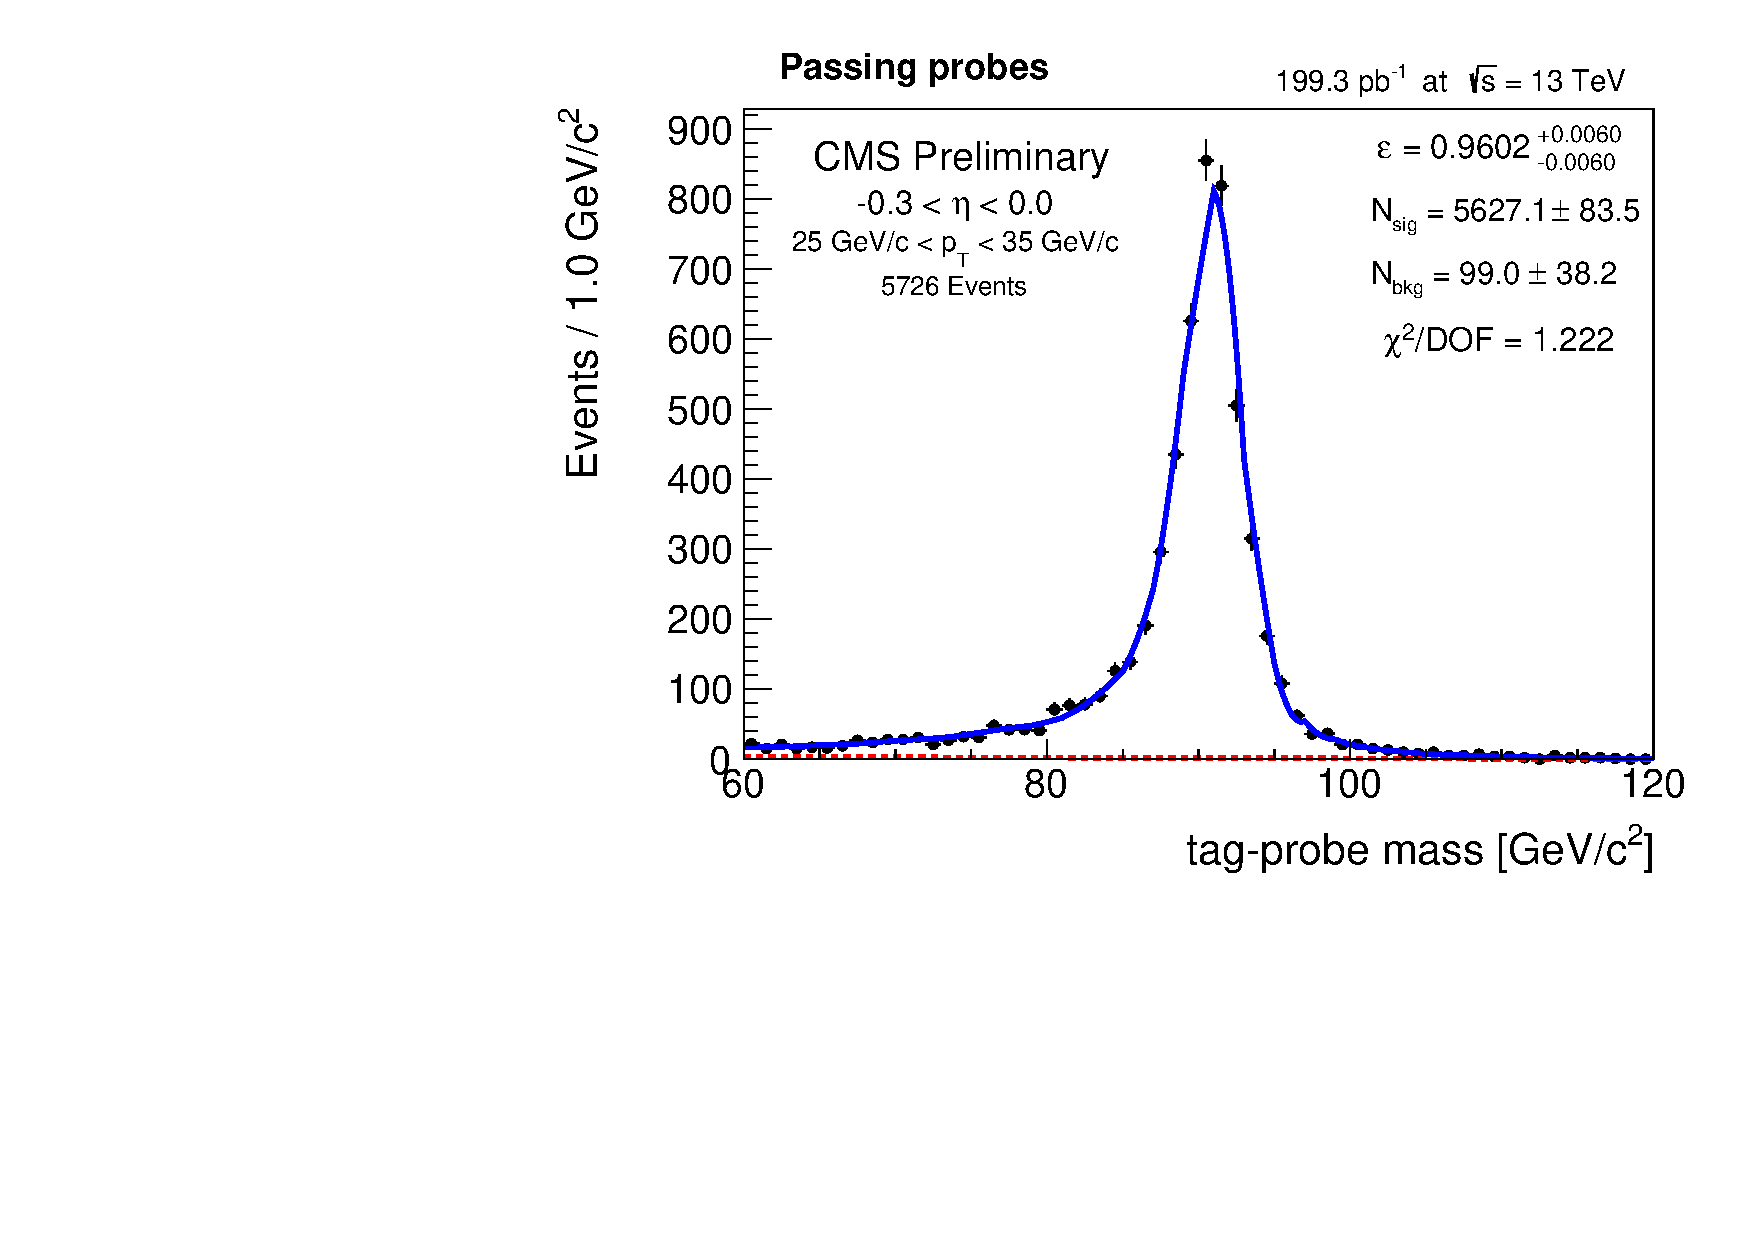
\includegraphics[width=.49\linewidth]{plots/efficiency/examples_musta/passetapt_5.pdf}
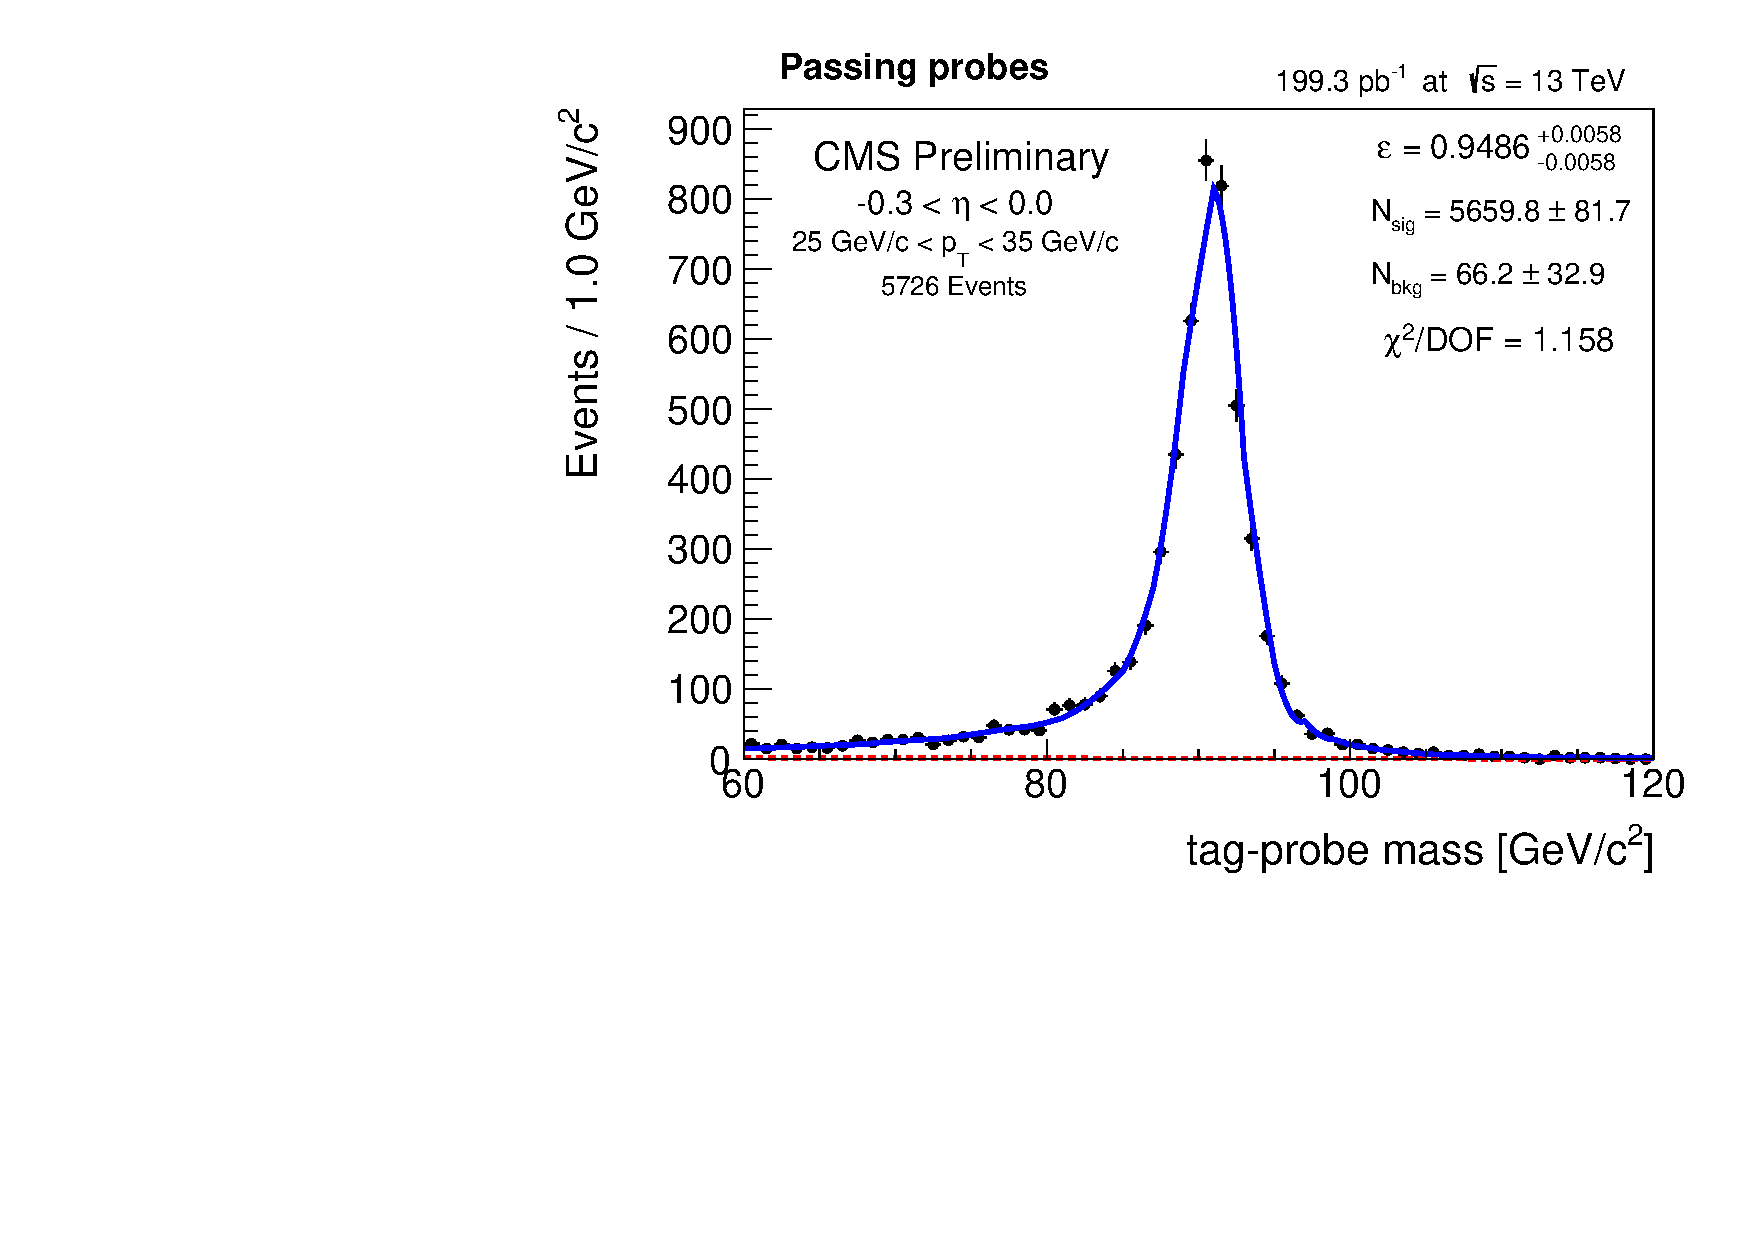
\includegraphics[width=.49\linewidth]{plots/efficiency/examples_plbkg/passetapt_5.pdf}
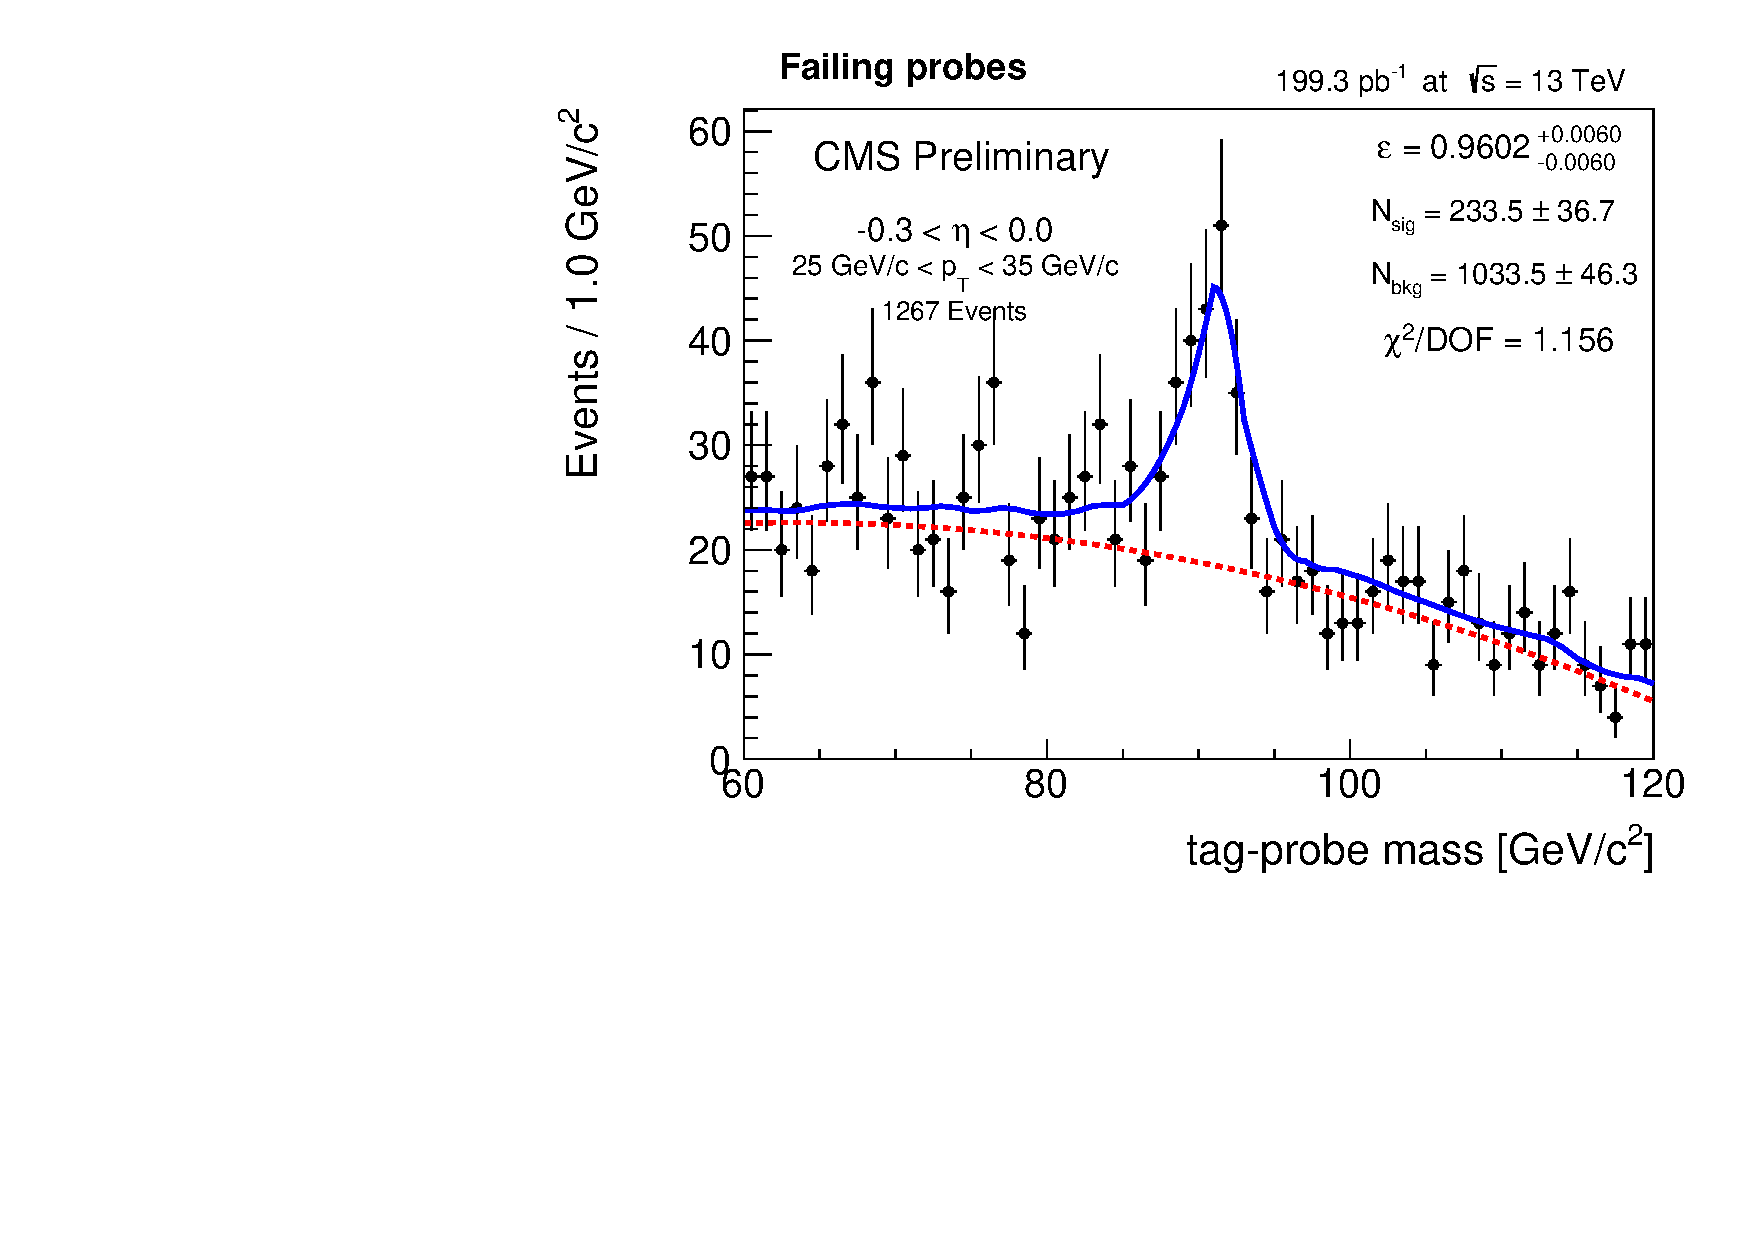
\includegraphics[width=.49\linewidth]{plots/efficiency/examples_musta/failetapt_5.pdf}
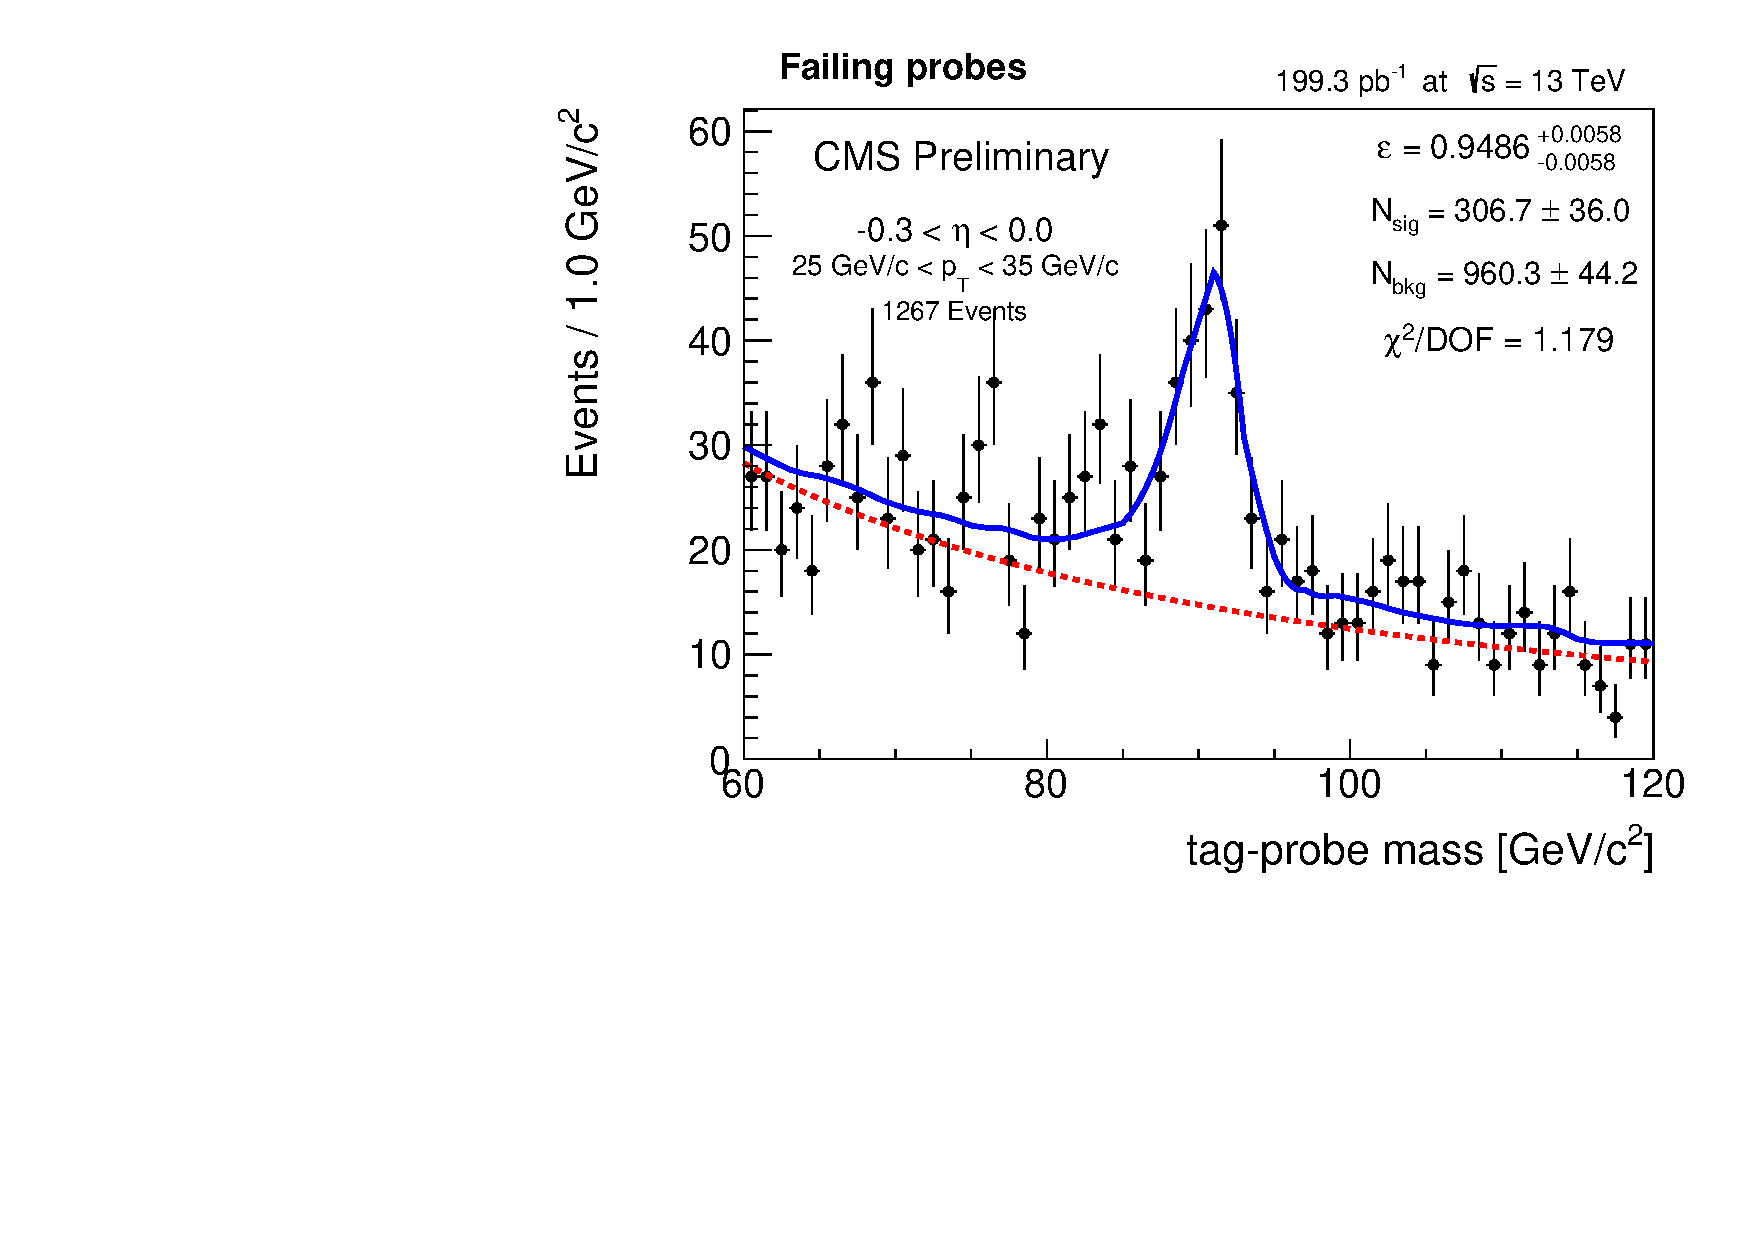
\includegraphics[width=.49\linewidth]{plots/efficiency/examples_plbkg/failetapt_5.pdf}
\caption{Examples of passing (top) and failing (bottom) probes from the same $p_T-\eta$ bin, from the muon standalone efficiency, fit with two different background models. The left plots use a quadratic polynomial and the right plots use a power law (shown in red).}
\label{fig:eff:musta:fitexample}
\end{figure}


\subsubsection{Tag Selection Uncertainty}
Uncertainty due to the selection criteria of the tag lepton are evaluated by directly comparing the impact of efficiency scale factors using the standard cut ($\pt > 25 \GeV$) to efficiency scale factors derived using tag leptons with $\pt > 30\GeV$. 

% \subsection{Summary of Systematic Uncertainties}
% A summary of the systematic uncertainties on the efficiency scale factors can be found in the Systematics Chapter later. 
% The impact of alternate models is evaluated by propagating the difference between models as a modification to the efficiency scale factor, and computing the selection-level acceptance with each of the alternative efficiency models. 
% Contributions of each type of systematic uncertainty are listed in the Tables ~\ref{tab:Eff:Unc:muon:summary:13} and ~\ref{tab:Eff:Unc:ele:summary:13} for 13 TeV and Table~\ref{tab:Eff:Unc:ele:summary:5} and Table~\ref{tab:Eff:Unc:mu:summary:5} for 5 TeV. 

\subsection{Statistical Uncertainty}
Statistical uncertainties in the efficiency scale factor are taken from the average over all variations on the measurement. The statistical uncertainty for a single $(\pt,\eta)$ bin is treated as Poisson, as given in Ref.~\cite{Paterno:2004cb}. Uncertainties for a given $(\pt,\eta)$ bin are correlated across all events containing leptons in the bin, while the uncertainties from separate $(\pt,\eta)$ bins are treated as uncorrelated. Individual categories (reconstruction, identification and isolation, trigger, etc.) are also treated as uncorrelated. The overall impact on the signal yield from the efficiency scale factor statistical uncertainties for the electron and muon channels in \serag and \serah are listed in Table~\ref{tab:eff:stat:all}.
%%%% Table containing the $e$ ID+Iso cuts
\begin{table}%[htbp]
\begin{center}

\scalebox{1.0}{
\begin{tabular}{|c|c|c|}
\hline
(13 TeV) & electron [\%] & muon [\%]\\
\hline \hline
$W^+$     & 0.489 & 0.291 \\
$W^-$     & 0.485 & 0.278 \\
$Z$       & 0.498 & 0.283 \\
\hline
\end{tabular} }
\quad
\scalebox{1.0}{
\begin{tabular}{|c|c|c|}
\hline
(5 TeV) & electron [\%] & muon [\%]\\
\hline \hline
$W^+$     & 0.489 & 0.245 \\
$W^-$     & 0.471 & 0.231\\
$Z$       & 0.526 & 0.268 \\
\hline
\end{tabular} }

\end{center}

\caption{Statistical uncertainty [\%] in the efficiency scale factor calculations on the \Wp, \Wm, and \Z boson acceptance at \sh (left) and \sg (right).}
\label{tab:eff:stat:all}
\end{table}

% \begin{table}[htbp]
\begin{center}
\begin{tabular}{ccccccccc}
\hline
Source & $W^+$& $W^-$ & $W$ & $W^+/W^-$ & $Z$ & $W^+/Z$&$W^+/Z$ &$W/Z$  \\
\hline \hline
FSR & 0.191 & 0.169 & 0.181 & 0.021 & 0.238 & 0.049 & 0.070 & 0.058 \\
MC & 0.073 & 0.067 & 0.070 & 0.006 & 0.094 & 0.023 & 0.029 & 0.025 \\
Background & 0.007 & 0.008 & 0.008 & 0.000 & 0.012 & 0.002 & 0.002 & 0.002 \\
Tag pT & 0.033 & 0.038 & 0.035 & 0.004 & 0.093 & 0.058 & 0.054 & 0.056 \\
Statistical & 0.286 & 0.278 & 0.202 & 0.009 & 0.279 & 0.008 & 0.001 & 0.076 \\
\hline \hline
Total [\%] & 0.35 & 0.33 & 0.28 & 0.00 & 0.39 & 0.07 & 0.08 & 0.10 \\

\end{tabular}
\end{center}
\caption{Uncertainties on the lepton efficiency scale factors for the muon channel in 13 TeV}
\label{tab:Eff:Unc:muon:summary:13}
\end{table}

% \begin{table}[htbp]
\begin{center}
\begin{tabular}{ccccccccc}
\hline
Source & $W^+$& $W^-$ & $W$ & $W^+/W^-$ & $Z$ & $W^+/Z$&$W^+/Z$ &$W/Z$  \\
\hline \hline
FSR & 0.081 & 0.080 & 0.081 & 0.001 & 0.166 & 0.087 & 0.089 & 0.085 \\
MC & 0.057 & 0.057 & 0.056 & 0.000 & 0.093 & 0.038 & 0.038 & 0.036 \\
Background & 0.056 & 0.053 & 0.055 & 0.004 & 0.099 & 0.041 & 0.044 & 0.045 \\
Tag pT & 0.016 & 0.018 & 0.017 & 0.001 & 0.047 & 0.066 & 0.067 & 0.063 \\
Statistical & 0.489 & 0.486 & 0.349 & 0.001 & 0.488 & 0.002 & 0.003 & 0.137 \\
\hline \hline
Total [\%] & 0.50 & 0.50 & 0.36 & 0.00 & 0.53 & 0.11 & 0.11 & 0.18 \\


\end{tabular}
\end{center}
\caption{Uncertainties on the lepton efficiency scale factors for the electron channel in 13 TeV}
\label{tab:Eff:Unc:ele:summary:13}
\end{table}
% %%%% Summary of lep eff systematics for muons - 5 TeV  %%%%%
\begin{table}[htbp]
\begin{center}
\begin{tabular}{ccccccccc}
\hline
Source & $W^+$& $W^-$ & $W$ & $W^+/W^-$ & $Z$ & $W^+/Z$&$W^+/Z$ &$W/Z$  \\
\hline \hline
MC & 0.09 & 0.08 & 0.09 & 0.00 & 0.15 & 0.07 & 0.07 & 0.07 \\
FSR & 0.17 & 0.15 & 0.32 & 0.01 & 0.27 & 0.23 & 0.26 & 0.24 \\
Bkg Model & 0.01 & 0.01 & 0.01 & 0.01 & 0.00 & 0.01 & 0.01 & 0.01 \\
Tag pT & 0.48 & 0.49 & 0.48 & 0.01 & 0.88 & 0.45 & 0.45 & 0.45 \\
stat & 0.25 & 0.24 & 0.20 & 0.32 & 0.26 & 0.38 & 0.36 & 0.35 \\
 \\
\hline \hline
Total [\%] & 0.56 & 0.56 & 0.61 & 0.32 & 0.96 & 0.62 & 0.62 & 0.61 \\
\end{tabular}
\end{center}
\caption{Summary of the propagated muon efficiency systematic uncertainties at 5 TeV.}
\label{tab:Eff:Unc:mu:summary:5}
\end{table}

% %%%% Summary of lep eff systematics for electrons - 5 TeV  %%%%%
\begin{table}%[htbp]
\begin{center}
\scalebox{0.7}{
\begin{tabular}{ccccccccc}
\hline
Source & $W^+$& $W^-$ & $W$ & $W^+/W^-$ & $Z$ & $W^+/Z$&$W^+/Z$ &$W/Z$  \\
\hline \hline
Binning [\%] & 0.00  & 0.00 & 0.00 & 0.00 & 0.00& 0.00& 0.00& 0.00\\
Signal Shape [\%] & 0.00  & 0.00 & 0.00 & 0.00 & 0.00& 0.00& 0.00& 0.00 \\
Background Shape [\%] & 0.00  & 0.00 & 0.00 & 0.00 & 0.00& 0.00& 0.00& 0.00  \\
\hline
\end{tabular}}
\end{center}
\caption{Summary of the propagated electron efficiency systematic uncertainties at 5 TeV.}
\label{tab:Eff:Unc:ele:summary:5}
\end{table}

% %%%% Summary of lep eff systematics for electrons - 13/5 TeV ratios  %%%%%
\begin{table}%[htbp]
\begin{center}
\scalebox{0.7}{
\begin{tabular}{ccccccccc}
\hline
Source & $W^+$& $W^-$ & $W$ & $W^+/W^-$ & $Z$ & $W^+/Z$&$W^+/Z$ &$W/Z$ \\
\hline \hline
Binning [\%] & 0.00  & 0.00 & 0.00 & 0.00 & 0.00& 0.00& 0.00& 0.00 \\
Signal Shape [\%] & 0.00  & 0.00 & 0.00 & 0.00 & 0.00& 0.00& 0.00& 0.00 \\
Background Shape [\%] & 0.00  & 0.00 & 0.00 & 0.00 & 0.00& 0.00& 0.00& 0.00  \\
\hline
\end{tabular}}
\end{center}
\caption{Summary of the propagated electron efficiency systematic uncertainties for the 13TeV/5TeV ratio.}
\label{tab:Eff:Unc:ele:summary:13to5}
\end{table}

% %%%% Summary of lep eff systematics for muons - 13/5 TeV ratios  %%%%%
\begin{table}%[htbp]
\begin{center}
\scalebox{0.7}{
\begin{tabular}{ccccccccc}
\hline
Source & $W^+$& $W^-$ & $W$ & $W^+/W^-$ & $Z$ & $W^+/Z$&$W^+/Z$ &$W/Z$  \\
\hline \hline
Binning [\%]          & 0.00  & 0.00 & 0.00 & 0.00 & 0.00& 0.00& 0.00 & 0.00 \\
Signal Shape [\%]     & 0.00  & 0.00 & 0.00 & 0.00 & 0.00& 0.00& 0.00 & 0.00 \\
Background Shape [\%] & 0.00  & 0.00 & 0.00 & 0.00 & 0.00& 0.00& 0.00 & 0.00  \\
\hline
\end{tabular}
}
\end{center}
\caption{Summary of the propagated muon efficiency systematic uncertainties for the 13 Tev/5 TeV ratio.}
\label{tab:Eff:Unc:mu:summary:13to5}
\end{table}




%% %%%%%%%%%%%%%%%%%%%%%%%%%%%
%%                Results
%%%%%%%%%%%%%%%%%%%%%%%%%%%%%
\section{Results}\label{ch:eff:results}
Distributions of $\eta$ dependence of efficiencies in data and simulation by $\pt$ bins for all lepton categories are provided, as well as tables containing total scale factors and statistical uncertainties. A list of tables and figures for \serag in Table~\ref{tab:eff:list:5} and for \serah is provided in Table~\ref{tab:eff:list:13}.
\begin{table}[htbp]
\begin{center}
\scalebox{1.0}{
\begin{tabular}{lcc}
\hline
Category [13 TeV] & Figure & Table   \\
\hline \hline
electron GSF+ID+Iso &  \ref{fig:Eff:el:13:GSFSel:com} &  \ref{tab:Eff:el:13TeV:GSFSel:com} \\
electron trigger & \ref{fig:Eff:el:13:HLT:pos}$(+)$,~ \ref{fig:Eff:el:13:HLT:neg}$(-)$ & \ref{tab:Eff:el:13TeV:HLT:pos}$(+)$,~\ref{tab:Eff:el:13TeV:HLT:neg}$(-)$ \\
muon Sel.+ID+Iso & \ref{fig:Eff:mu:13:SIT:com} & \ref{tab:Eff:mu:13TeV:SIT:com} \\
muon standalone & \ref{fig:Eff:mu:13:Sta:com}  & \ref{tab:Eff:mu:13TeV:Sta:com} \\
muon trigger &\ref{fig:Eff:mu:13:HLT:pos}$(+)$,~\ref{fig:Eff:mu:13:HLT:neg}$(-)$ & \ref{tab:Eff:mu:13TeV:HLT:pos}$(+)$,~\ref{tab:Eff:mu:13TeV:HLT:neg}$(-)$ \\
\hline
Category [5 TeV] & Figure & Table   \\
\hline \hline
electron GSF+ID+Iso &  \ref{fig:Eff:el:5:GSFSel:com} &  \ref{tab:Eff:el:5TeV:GSFSel:com} \\
electron trigger & \ref{fig:Eff:el:5:HLT:pos}$(+)$,~ \ref{fig:Eff:el:5:HLT:neg}$(-)$ & \ref{tab:Eff:el:5TeV:HLT:pos}$(+)$,~\ref{tab:Eff:el:5TeV:HLT:neg}$(-)$ \\
muon Sel.+ID+Iso & \ref{fig:Eff:mu:5:SIT:com} & \ref{tab:Eff:mu:5TeV:SIT:com} \\
muon standalone & \ref{fig:Eff:mu:5:Sta:com}  & \ref{tab:Eff:mu:13TeV:Sta:com} \\
muon trigger &\ref{fig:Eff:mu:5:HLT:pos}$(+)$,~\ref{fig:Eff:mu:5:HLT:neg}$(-)$ & \ref{tab:Eff:mu:5TeV:HLT:pos}$(+)$,~\ref{tab:Eff:mu:5TeV:HLT:neg}$(-)$ \\
\hline
\end{tabular}}
\end{center}
\caption{List of tables and figures containing \serag and \serah lepton efficiency scale factors.}
\label{tab:eff:list}
\end{table}

% % 13 TeV electrons
%%%% Figures for EleGSFSel Efficiency  %%%%%
\begin{figure}
\centering
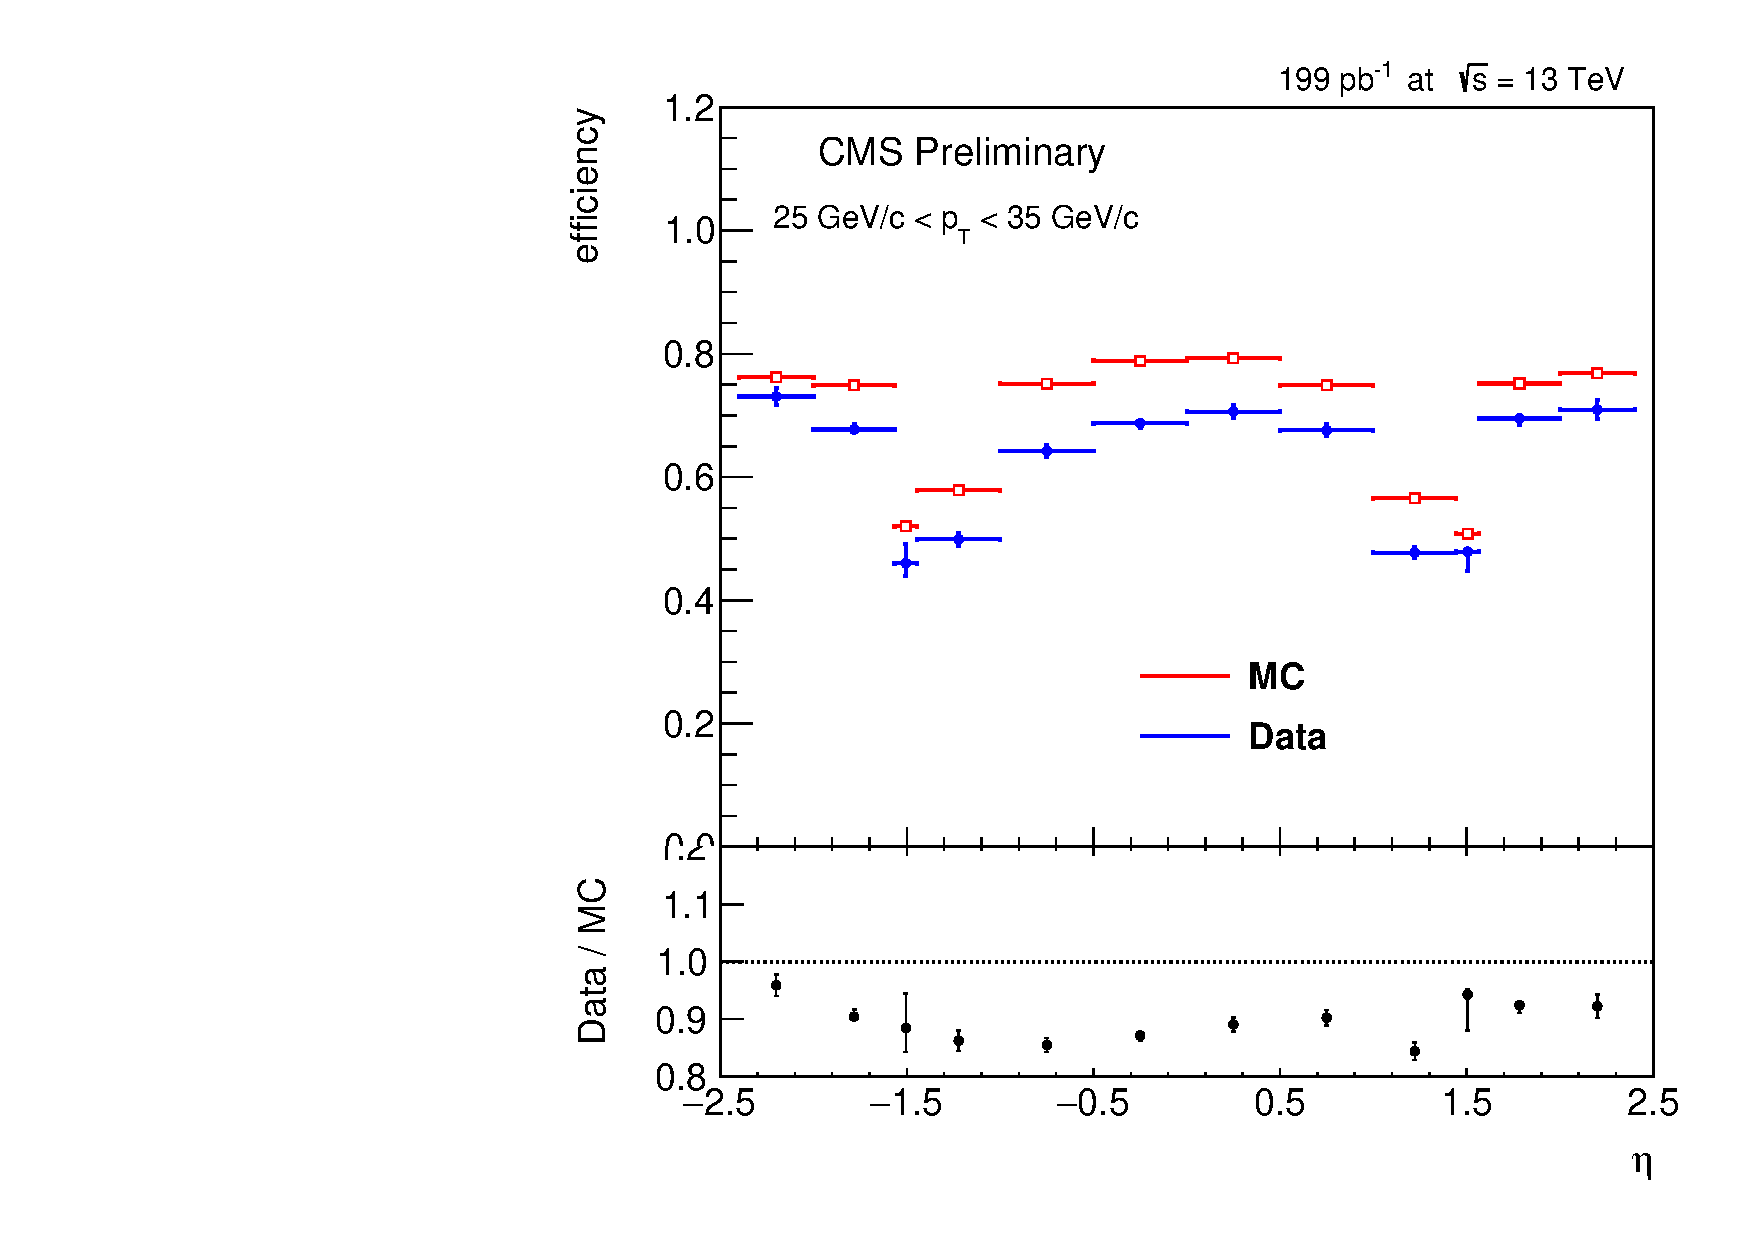
\includegraphics[width=0.48\linewidth]{plots/efficiency/13_zeegsfsel_combined/PtBins_eta_pt0.pdf}
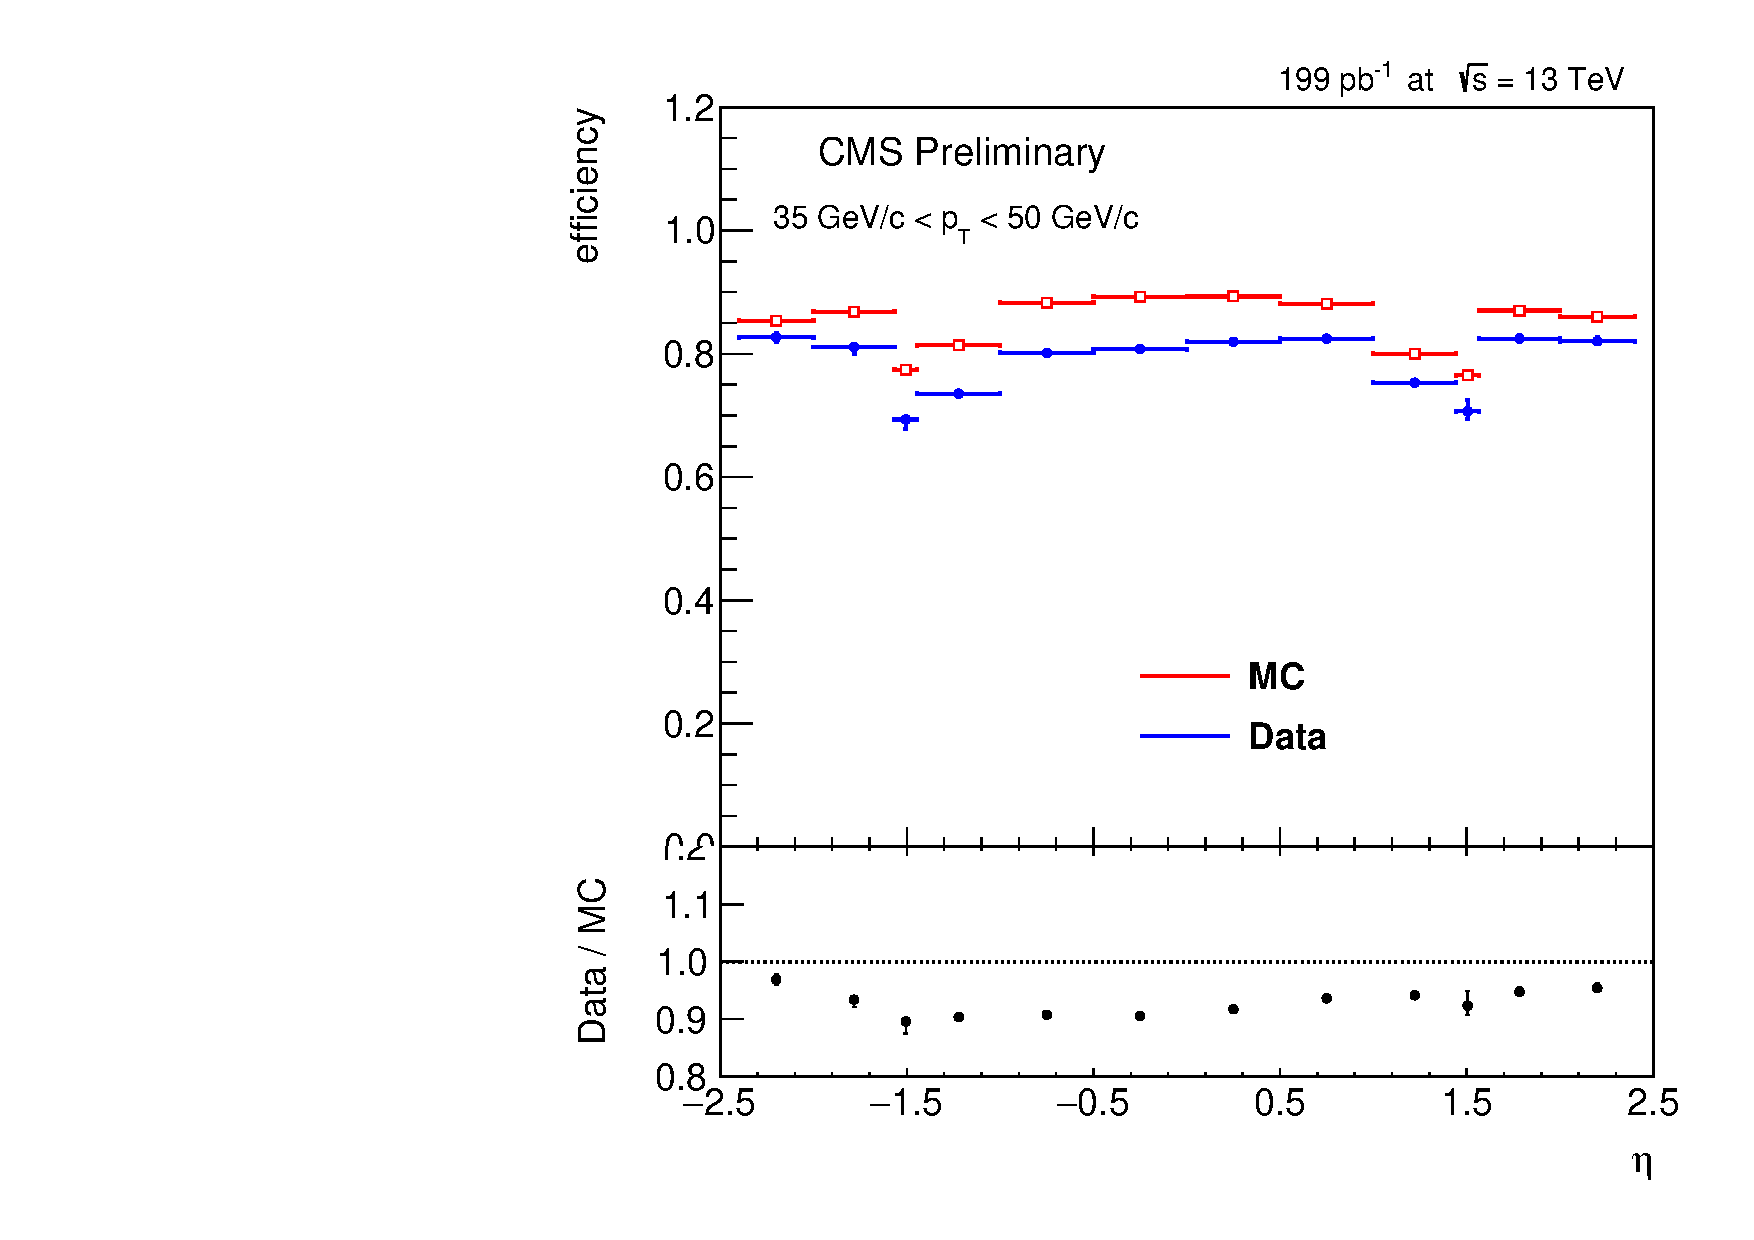
\includegraphics[width=0.48\linewidth]{plots/efficiency/13_zeegsfsel_combined/PtBins_eta_pt1.pdf}
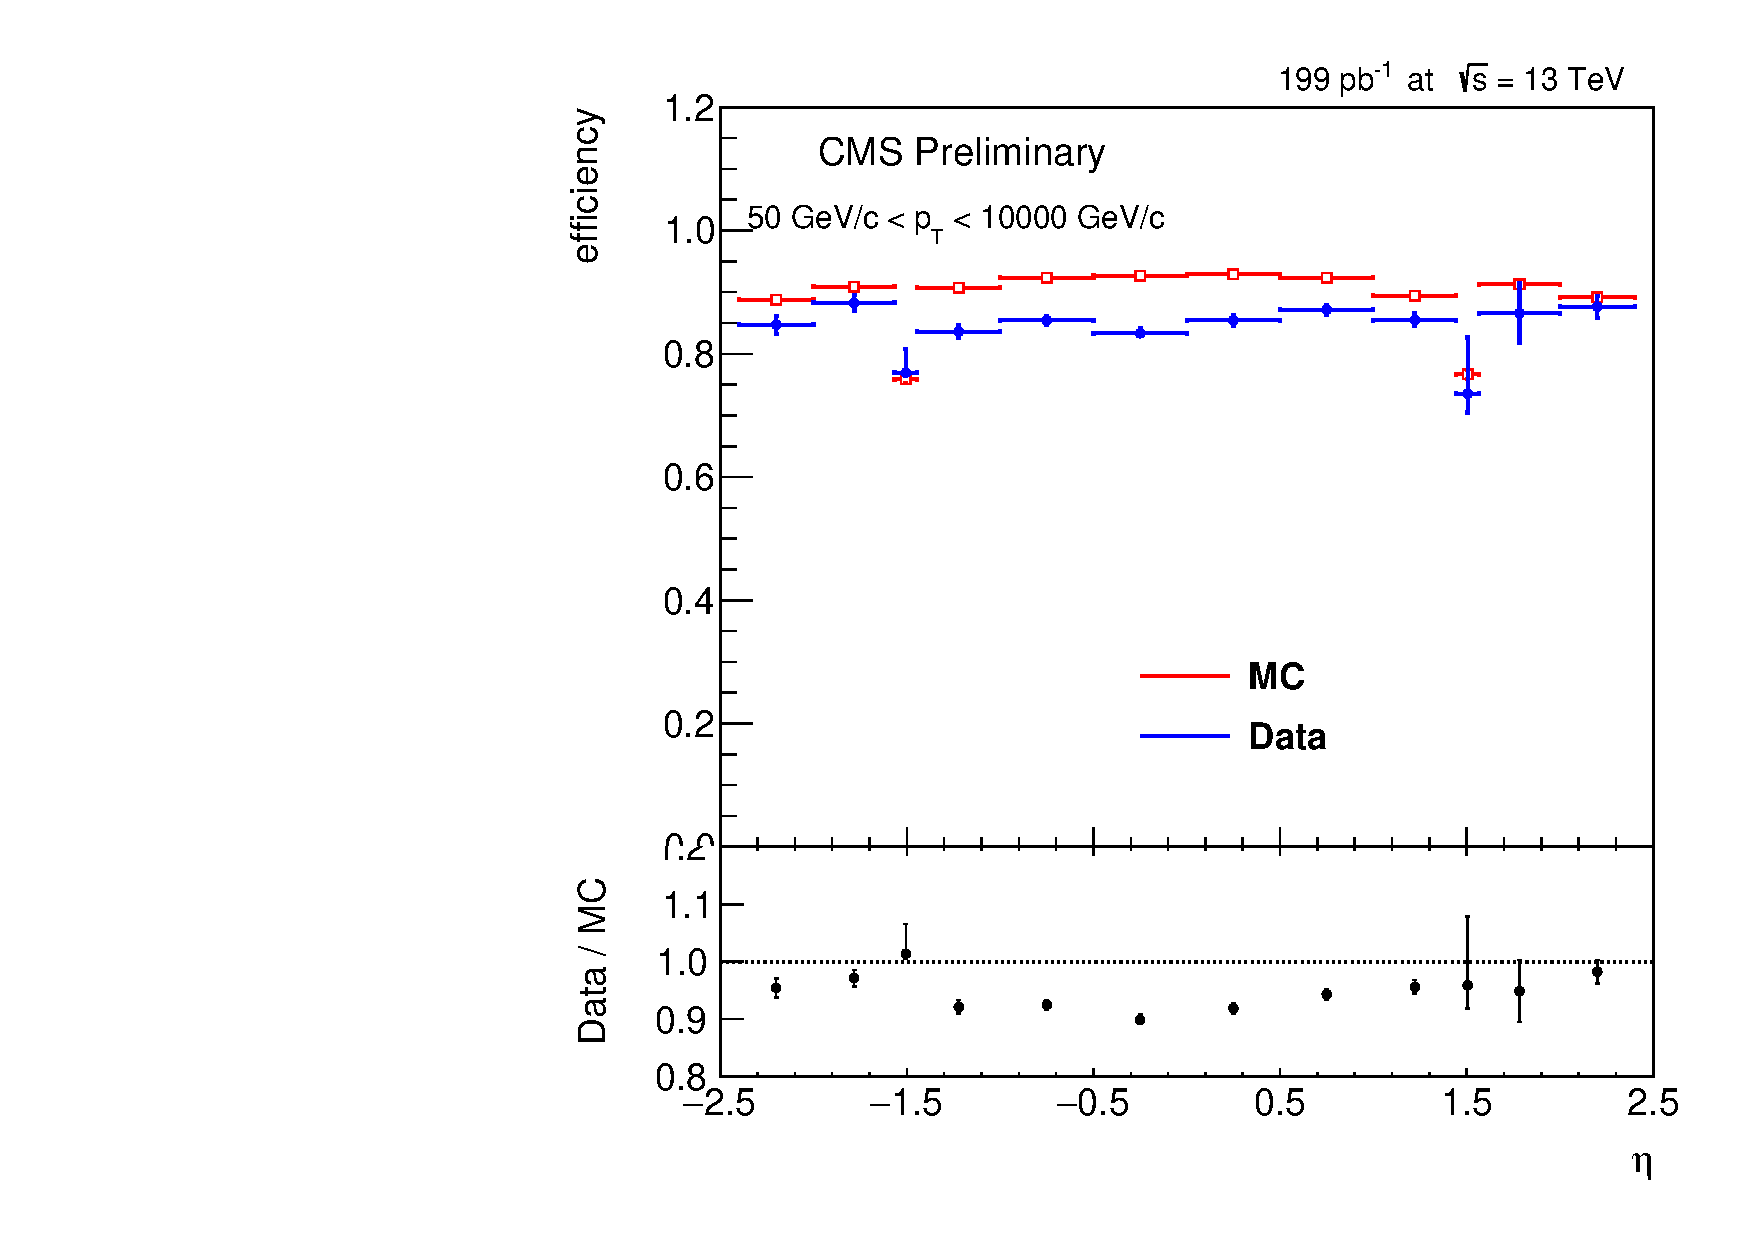
\includegraphics[width=0.48\linewidth]{plots/efficiency/13_zeegsfsel_combined/PtBins_eta_pt2.pdf}
\caption{$\eta$ dependence of GSF electron identification and isolation efficiency scale factors, separated by $p_T$ bins, for combined charged electrons in the 13 TeV samples.}
\label{fig:Eff:el:13:GSFSel:com}
\end{figure}

%%%% Figures for EleHLT Efficiency  %%%%%
\begin{figure}
\centering
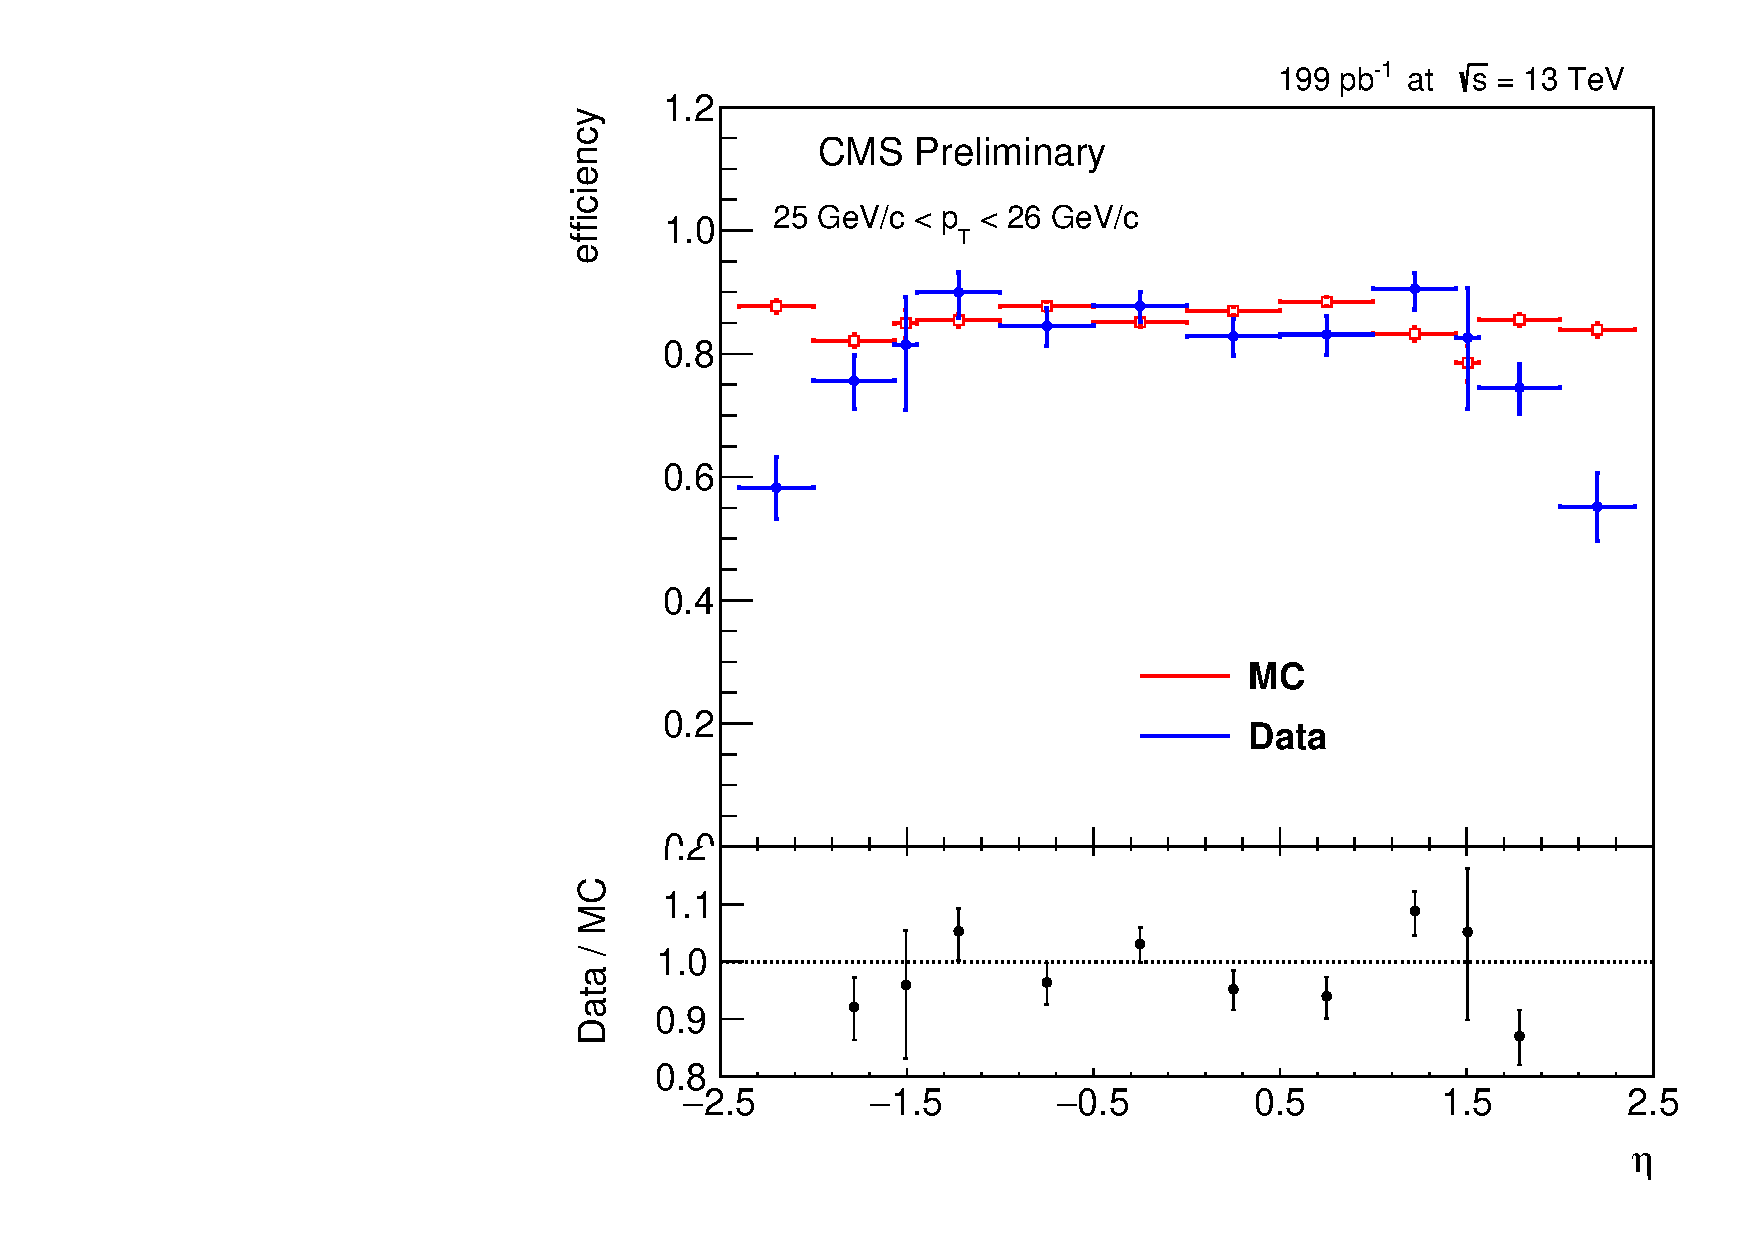
\includegraphics[width=0.45\linewidth]{plots/efficiency/13_zeehlt_positive/PtBins_eta_pt0.pdf}
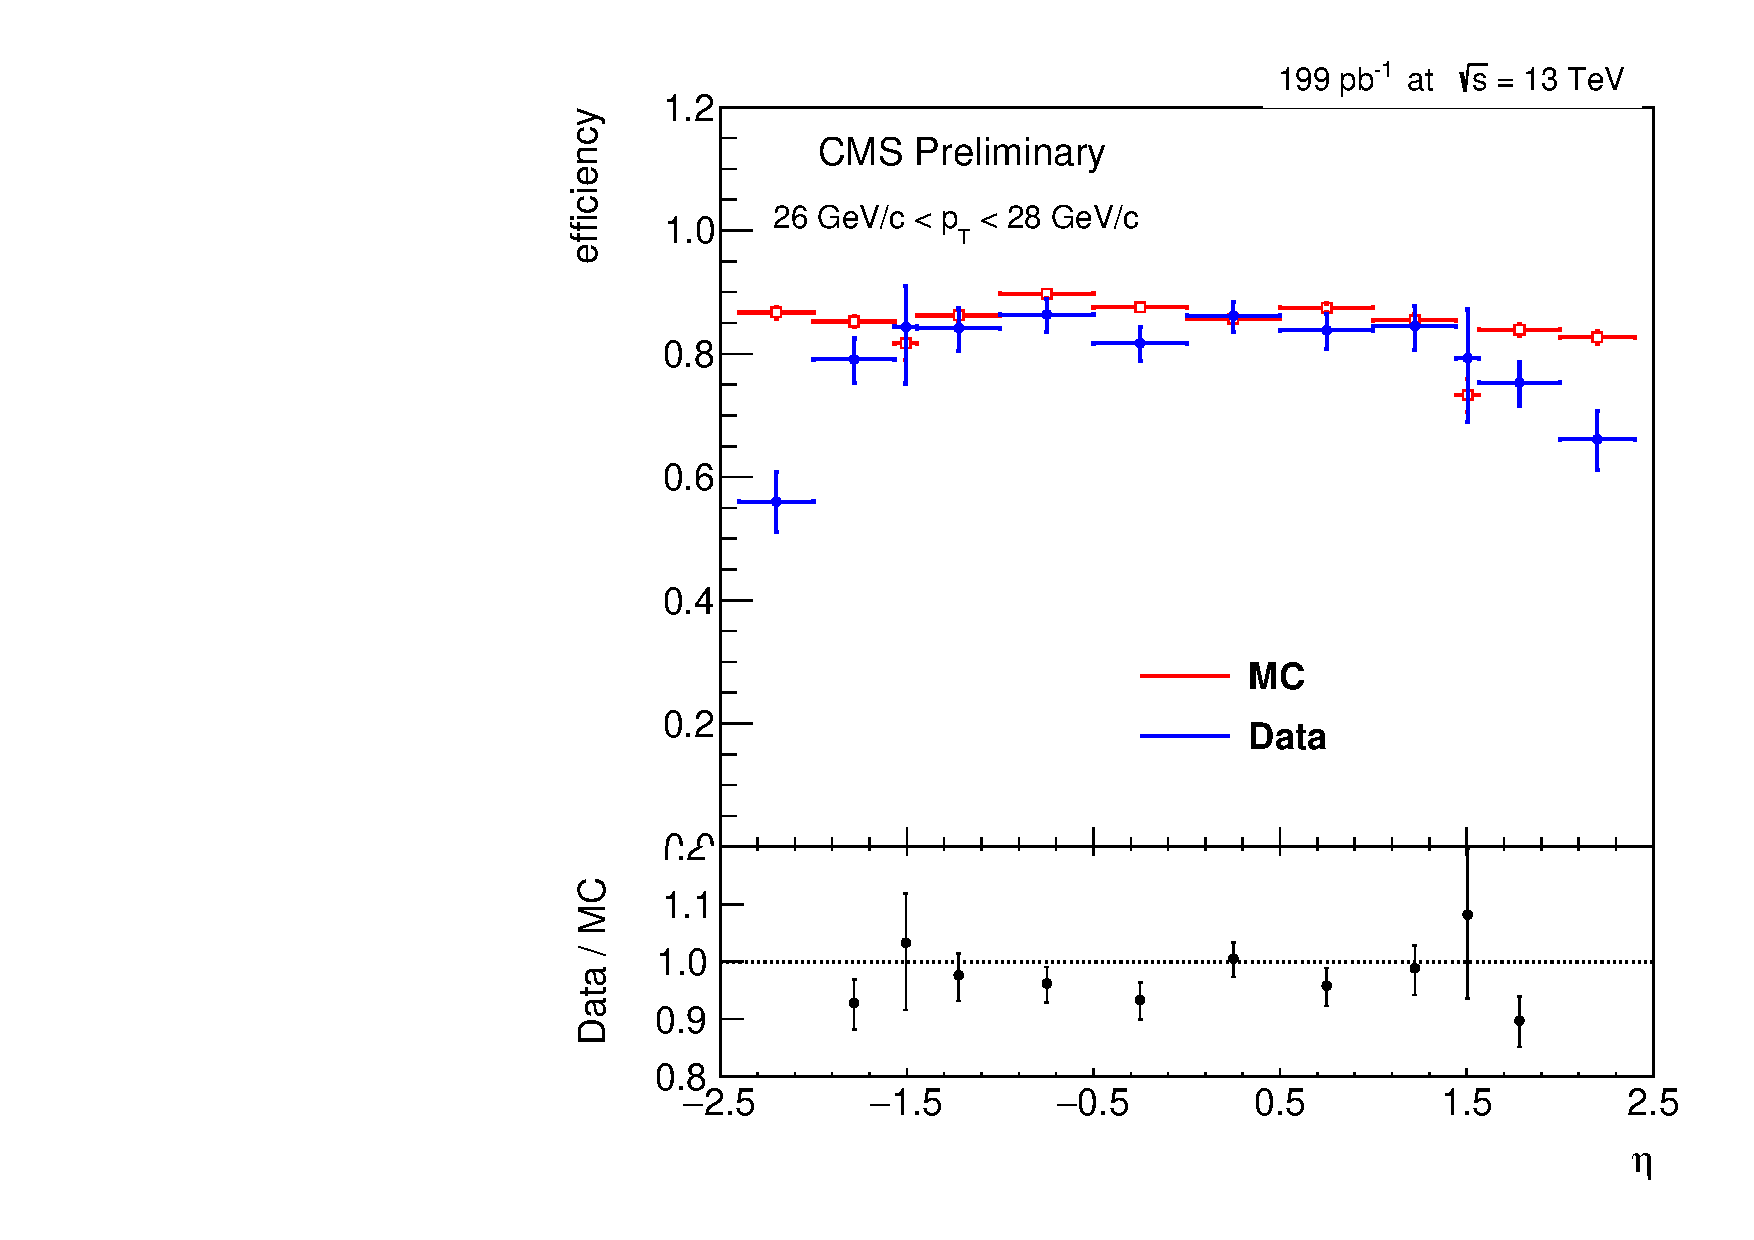
\includegraphics[width=0.45\linewidth]{plots/efficiency/13_zeehlt_positive/PtBins_eta_pt1.pdf}
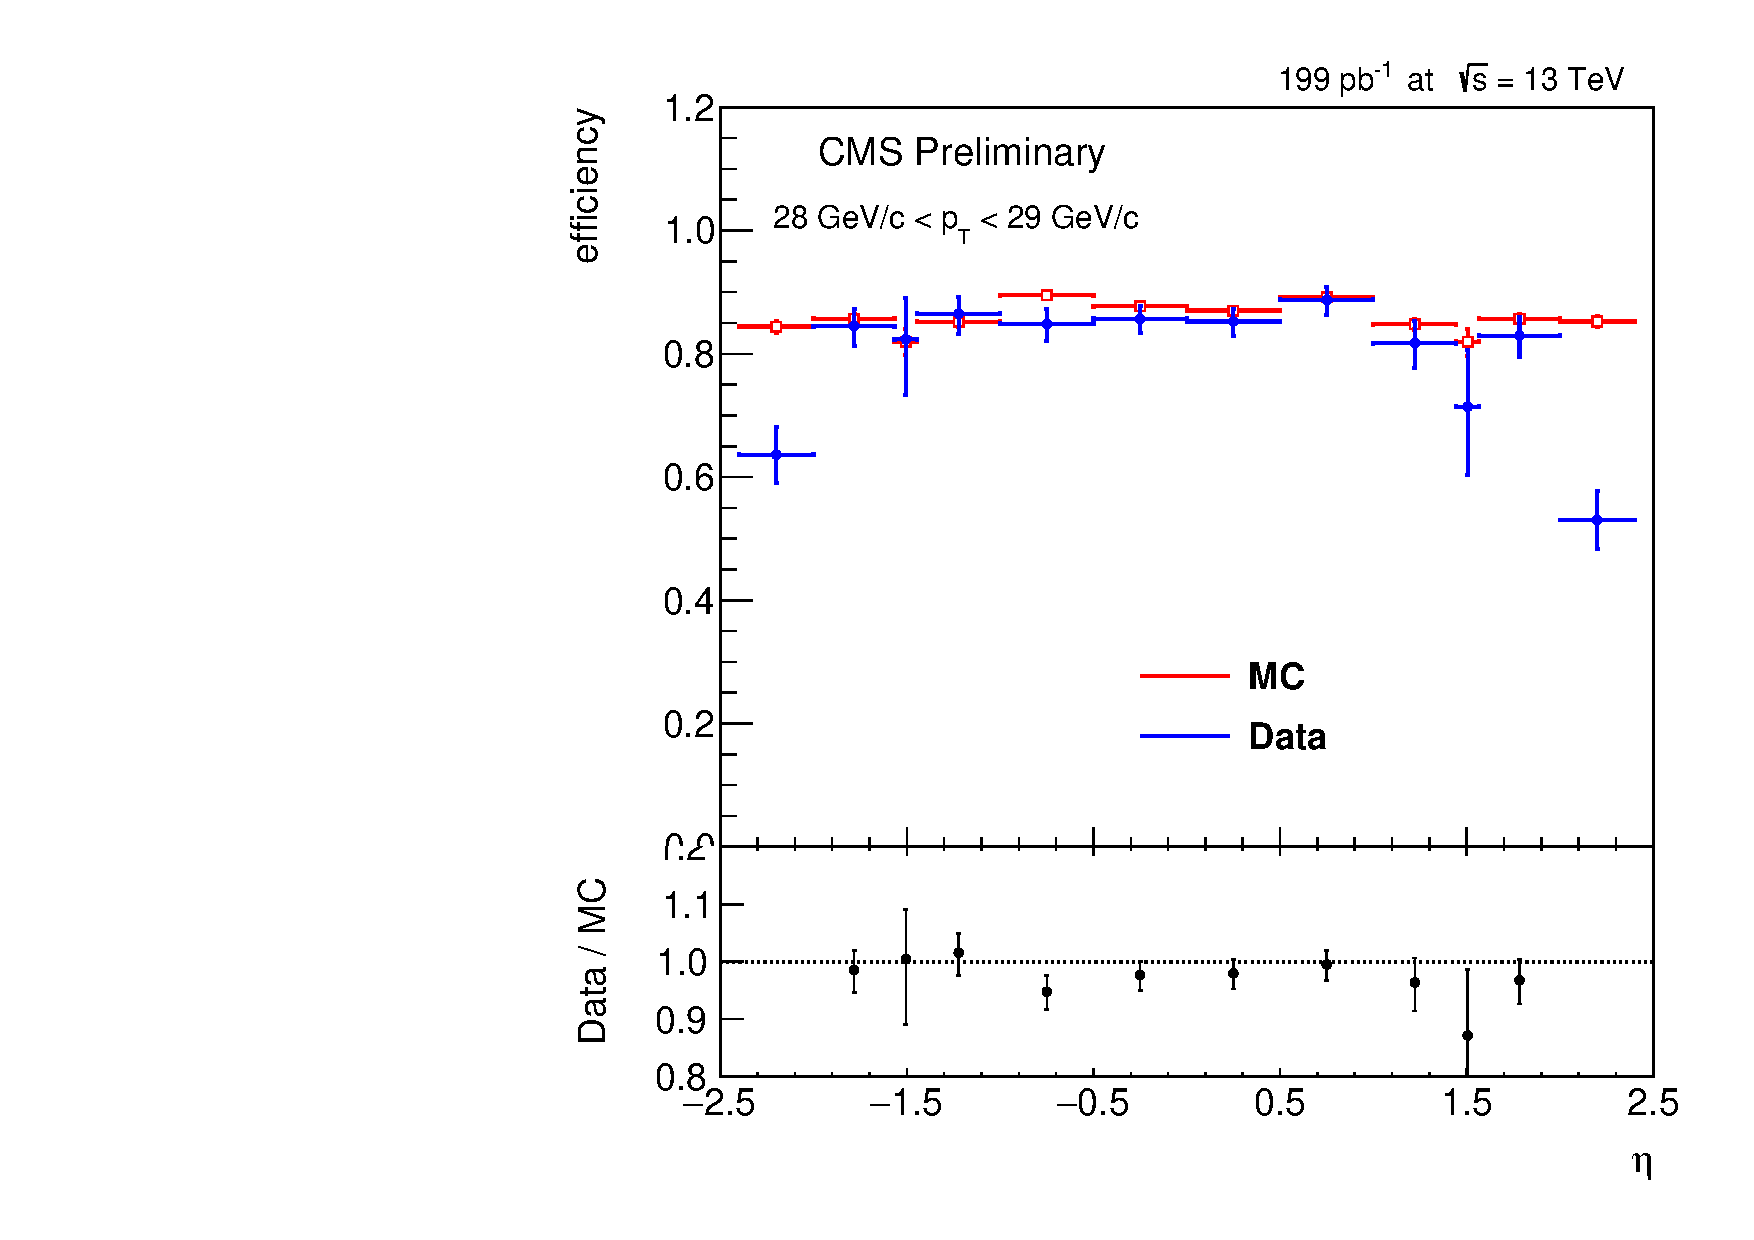
\includegraphics[width=0.45\linewidth]{plots/efficiency/13_zeehlt_positive/PtBins_eta_pt2.pdf}
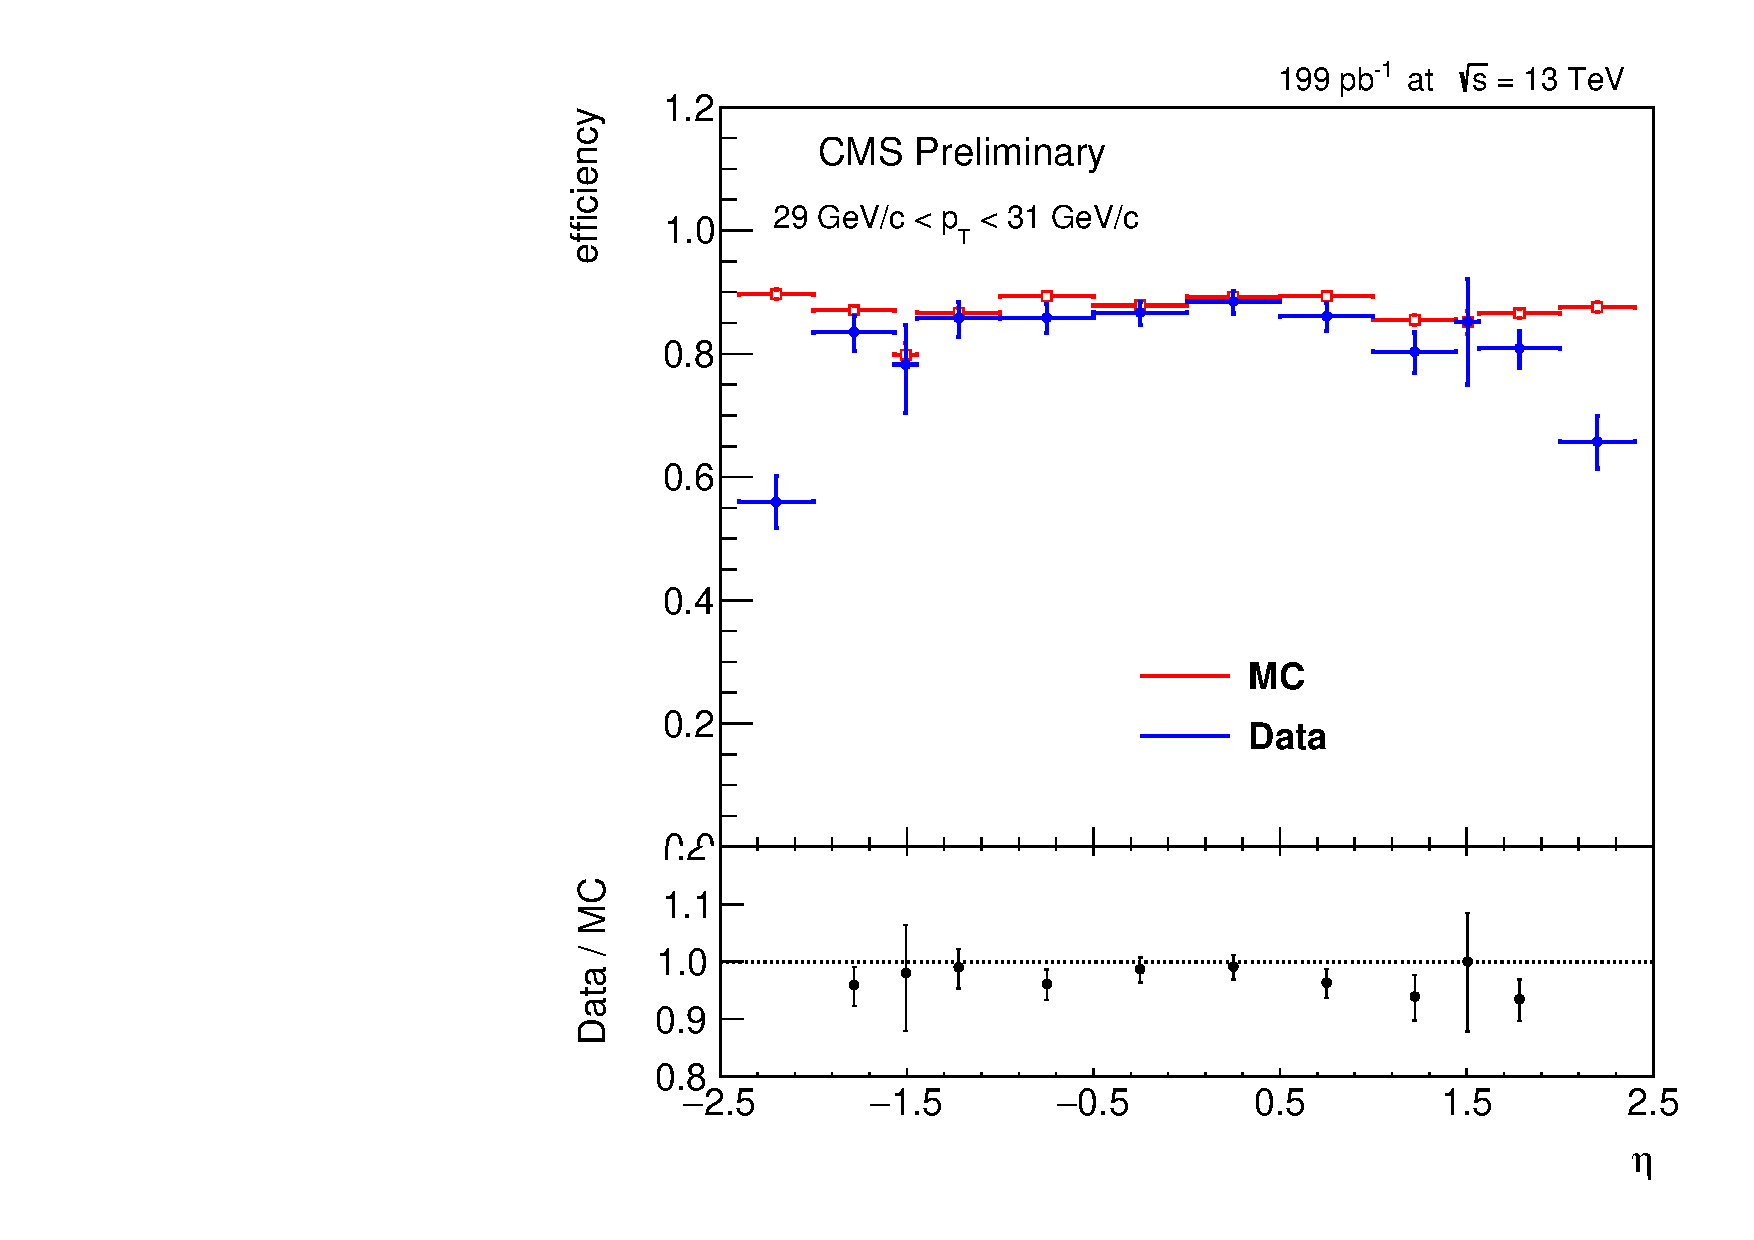
\includegraphics[width=0.45\linewidth]{plots/efficiency/13_zeehlt_positive/PtBins_eta_pt3.pdf}
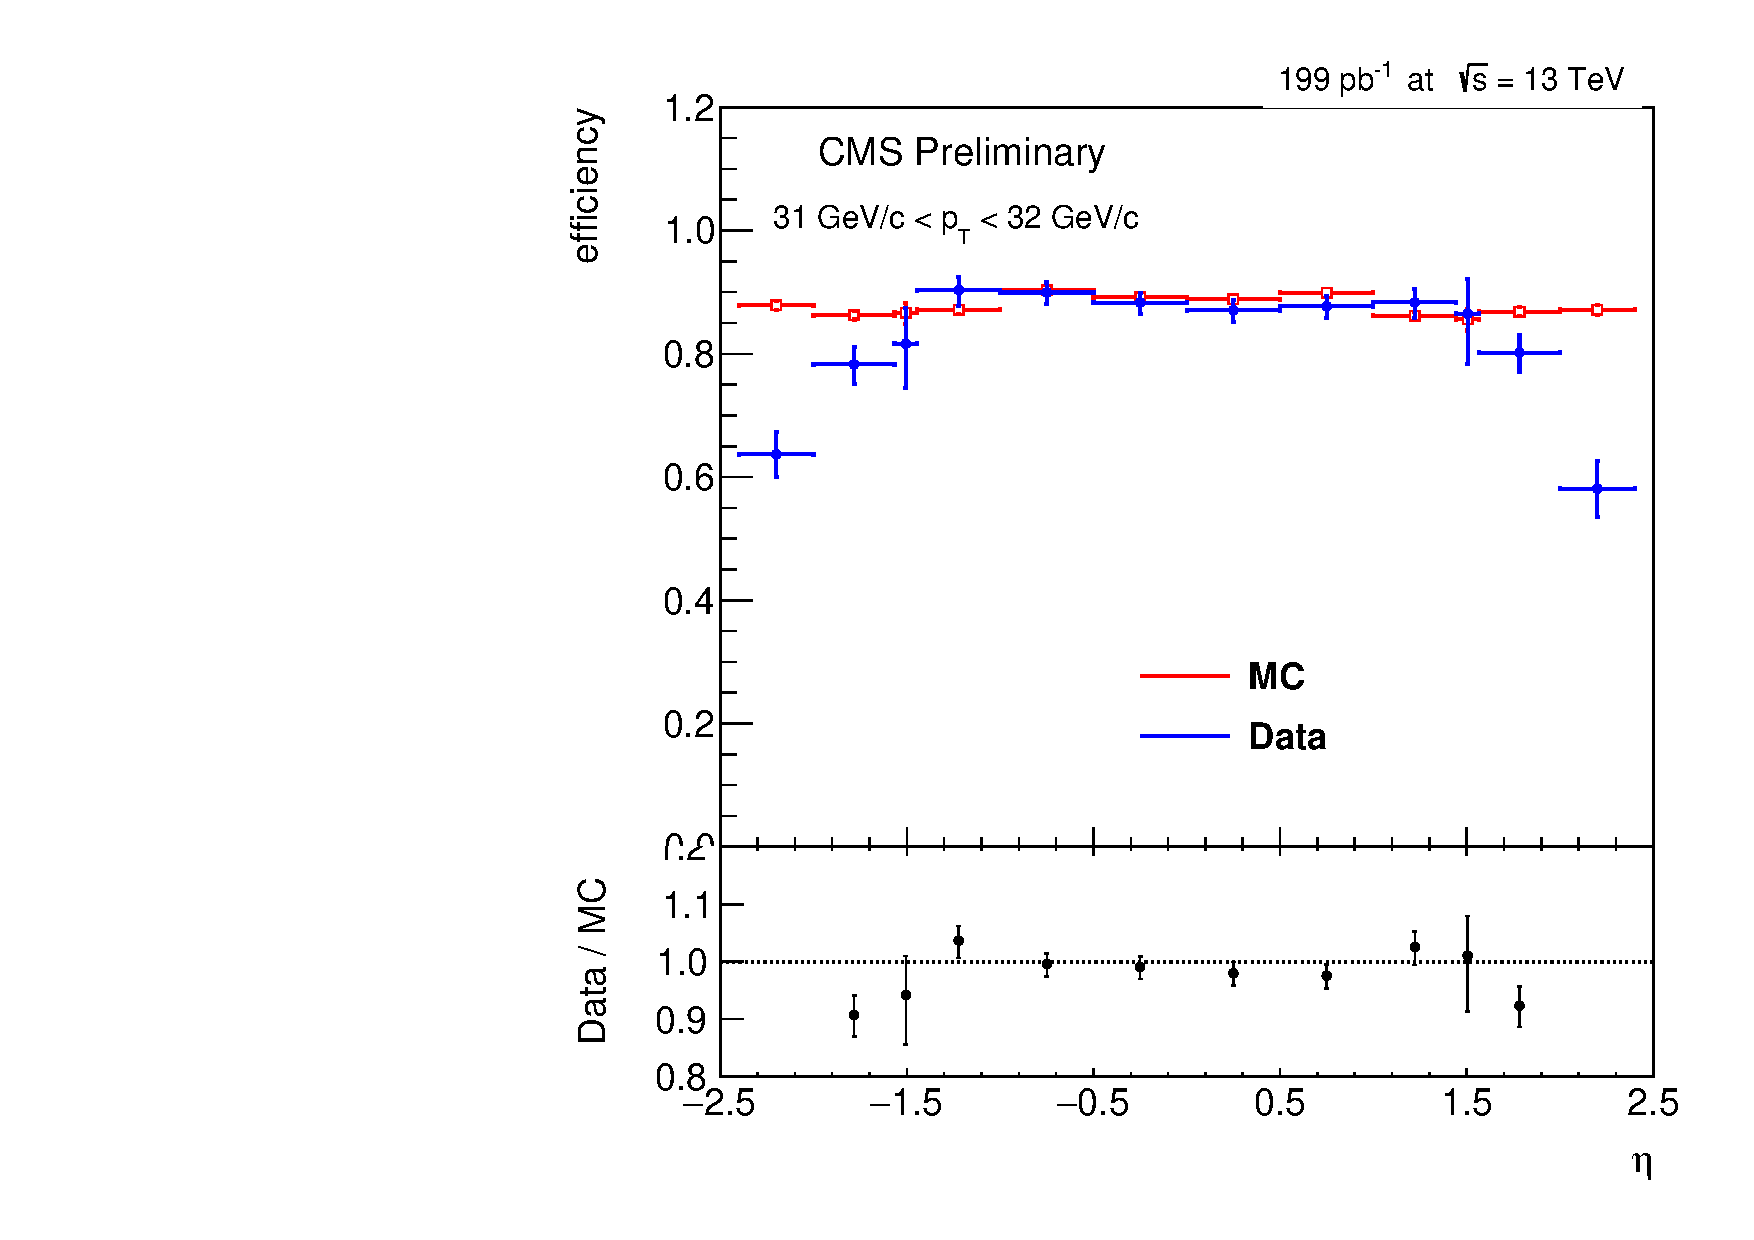
\includegraphics[width=0.45\linewidth]{plots/efficiency/13_zeehlt_positive/PtBins_eta_pt4.pdf}
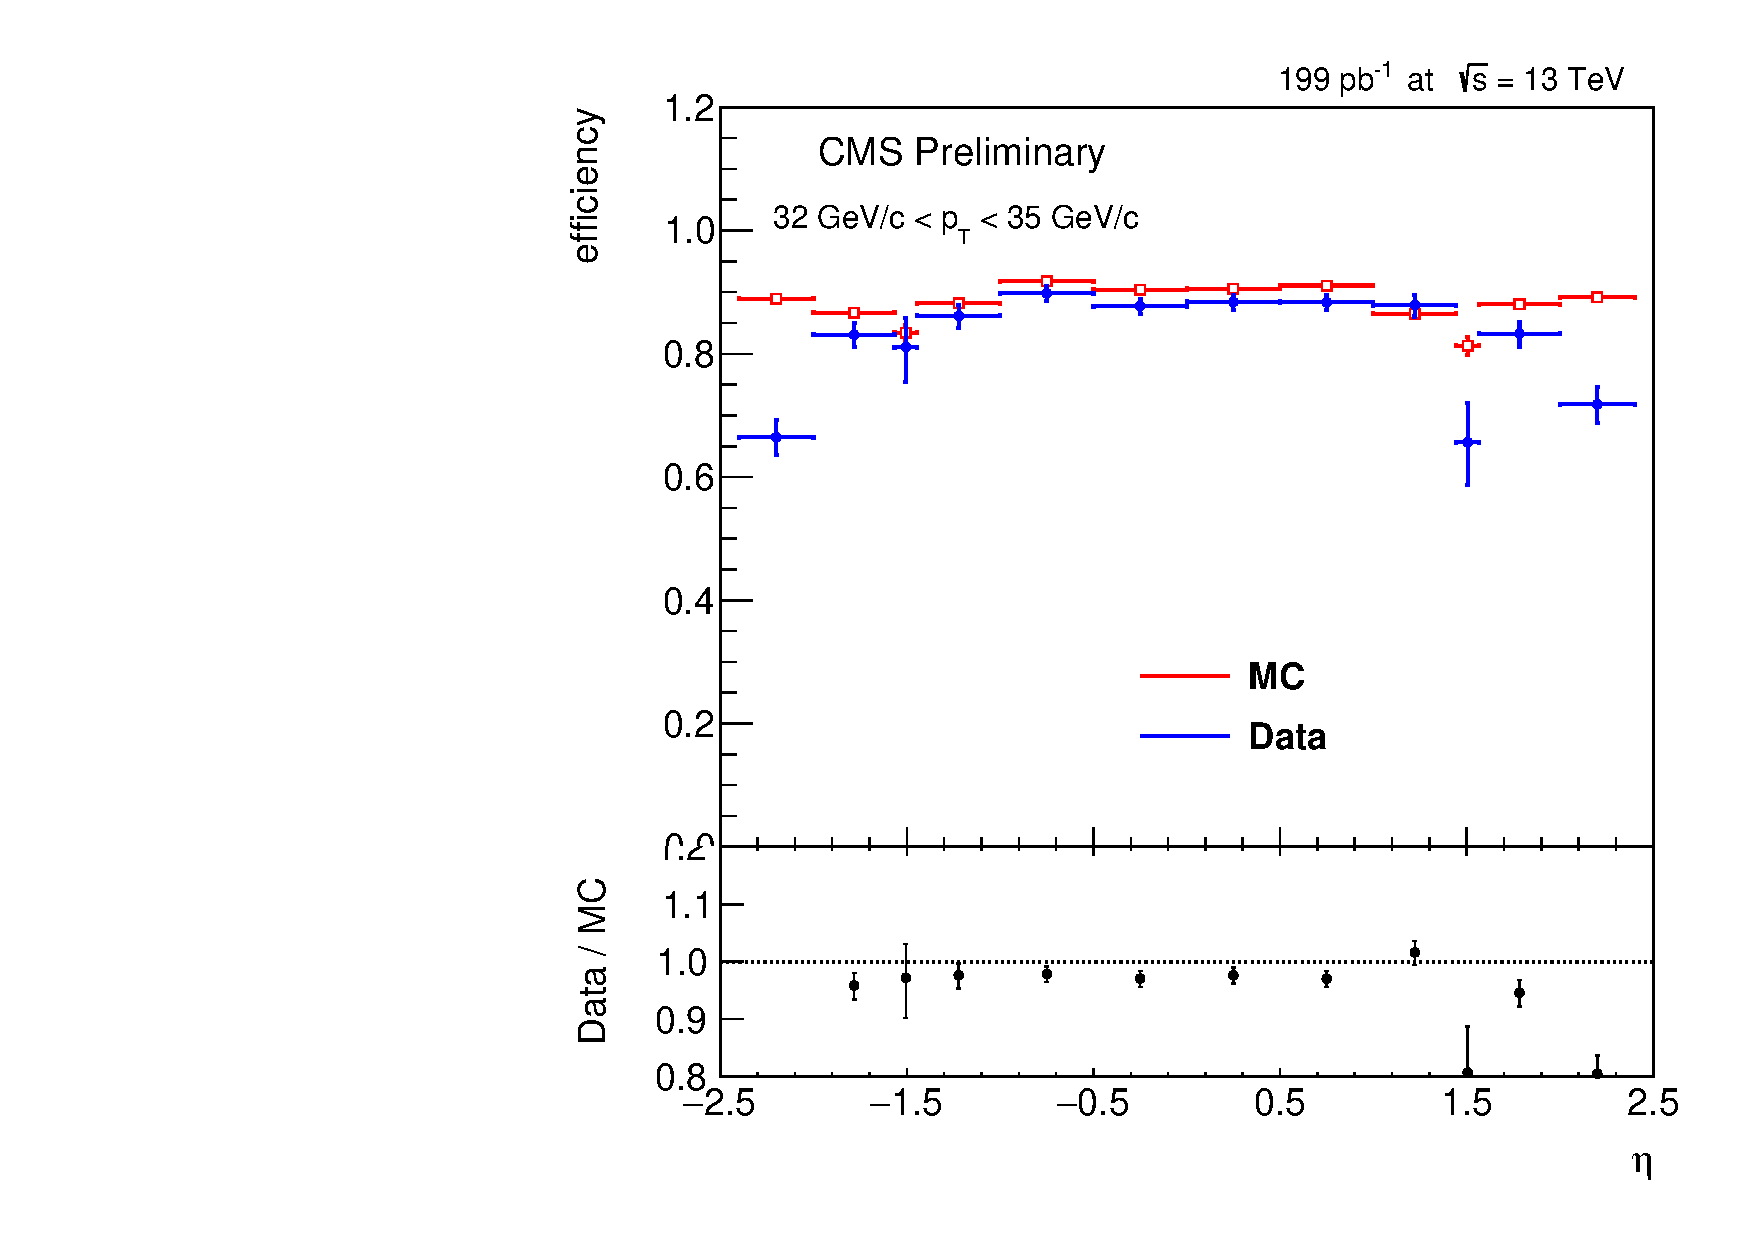
\includegraphics[width=0.45\linewidth]{plots/efficiency/13_zeehlt_positive/PtBins_eta_pt5.pdf}
\caption{$\eta$ dependence of Single electron trigger efficiency scale factors, separated by $p_T$ bins, for positively charged electrons in the 13 TeV samples.}
% \label{fig:Eff:el:13:HLT:pos}
\end{figure}
\begin{figure}
\ContinuedFloat
\centering
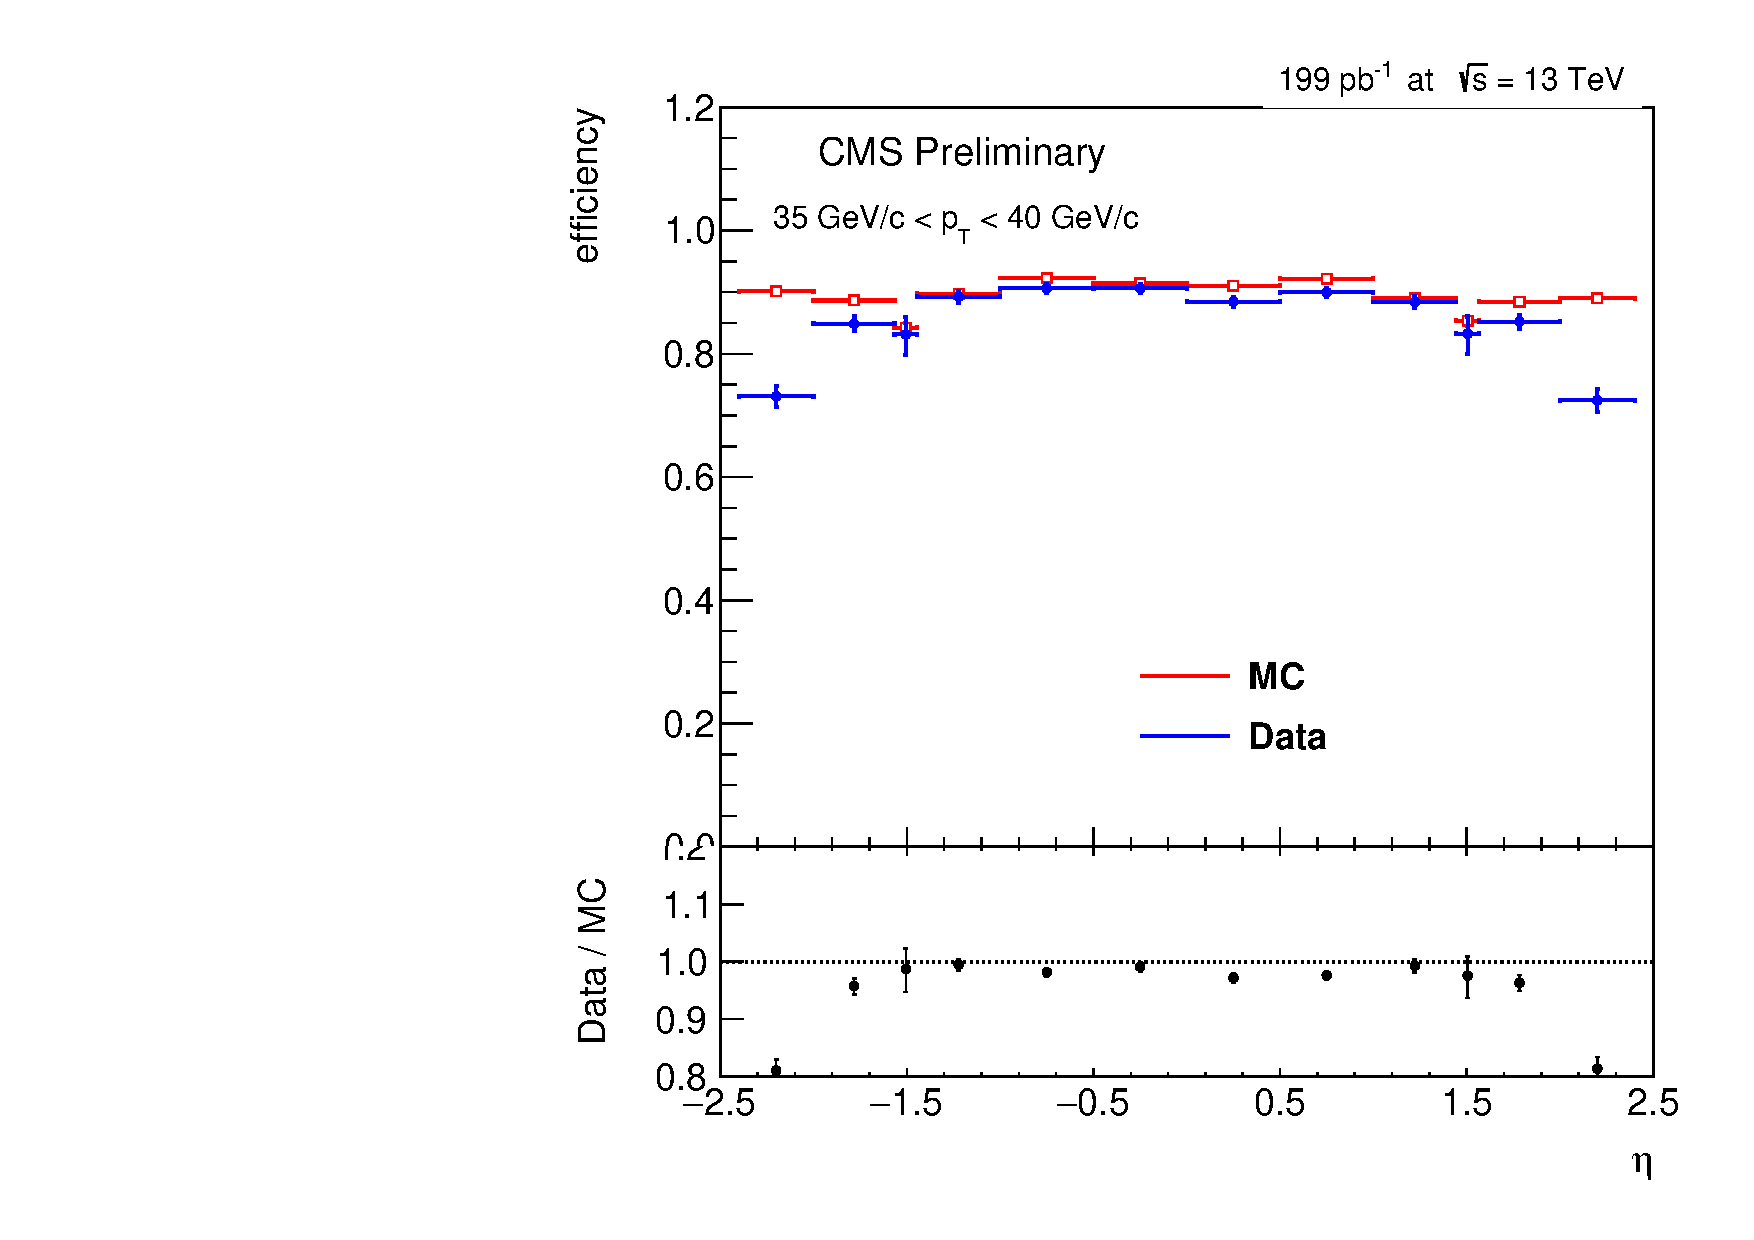
\includegraphics[width=0.45\linewidth]{plots/efficiency/13_zeehlt_positive/PtBins_eta_pt6.pdf}
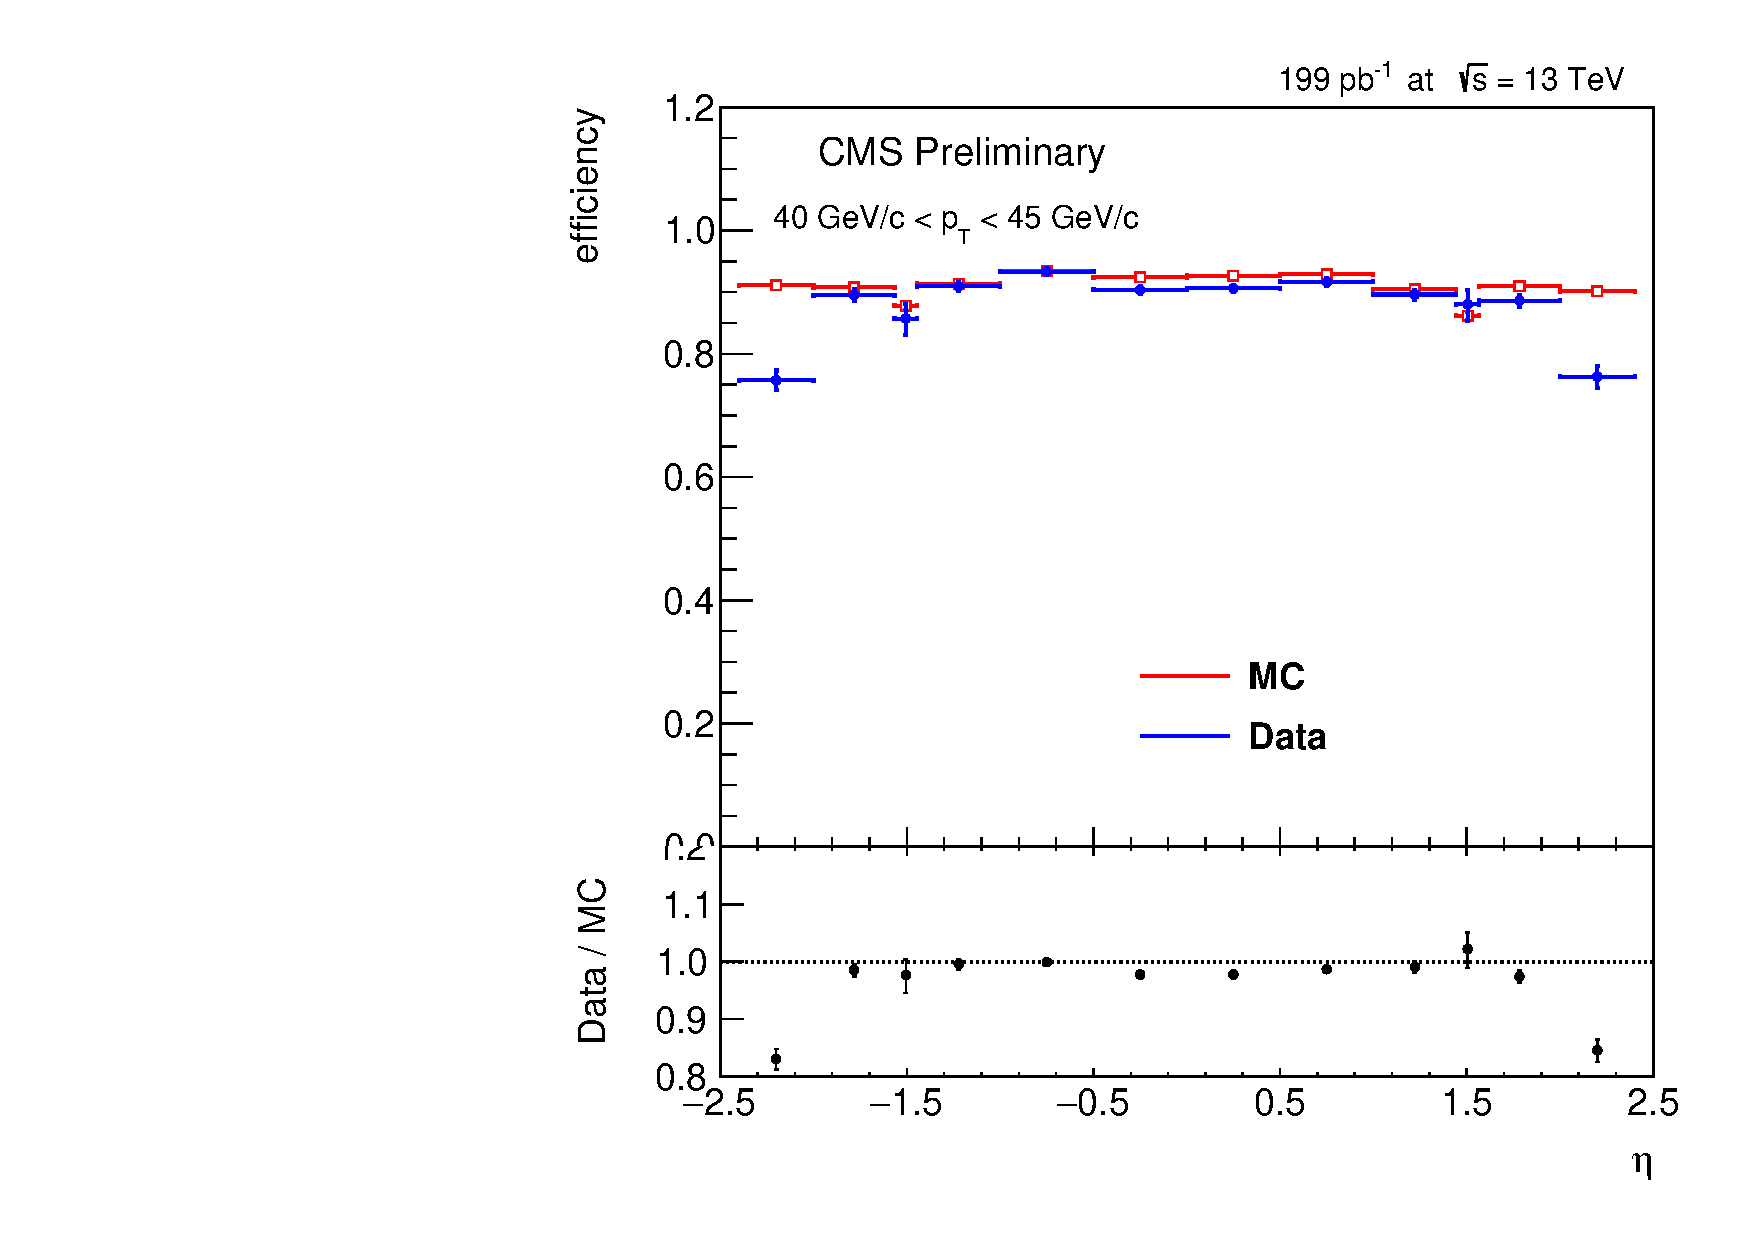
\includegraphics[width=0.45\linewidth]{plots/efficiency/13_zeehlt_positive/PtBins_eta_pt7.pdf}
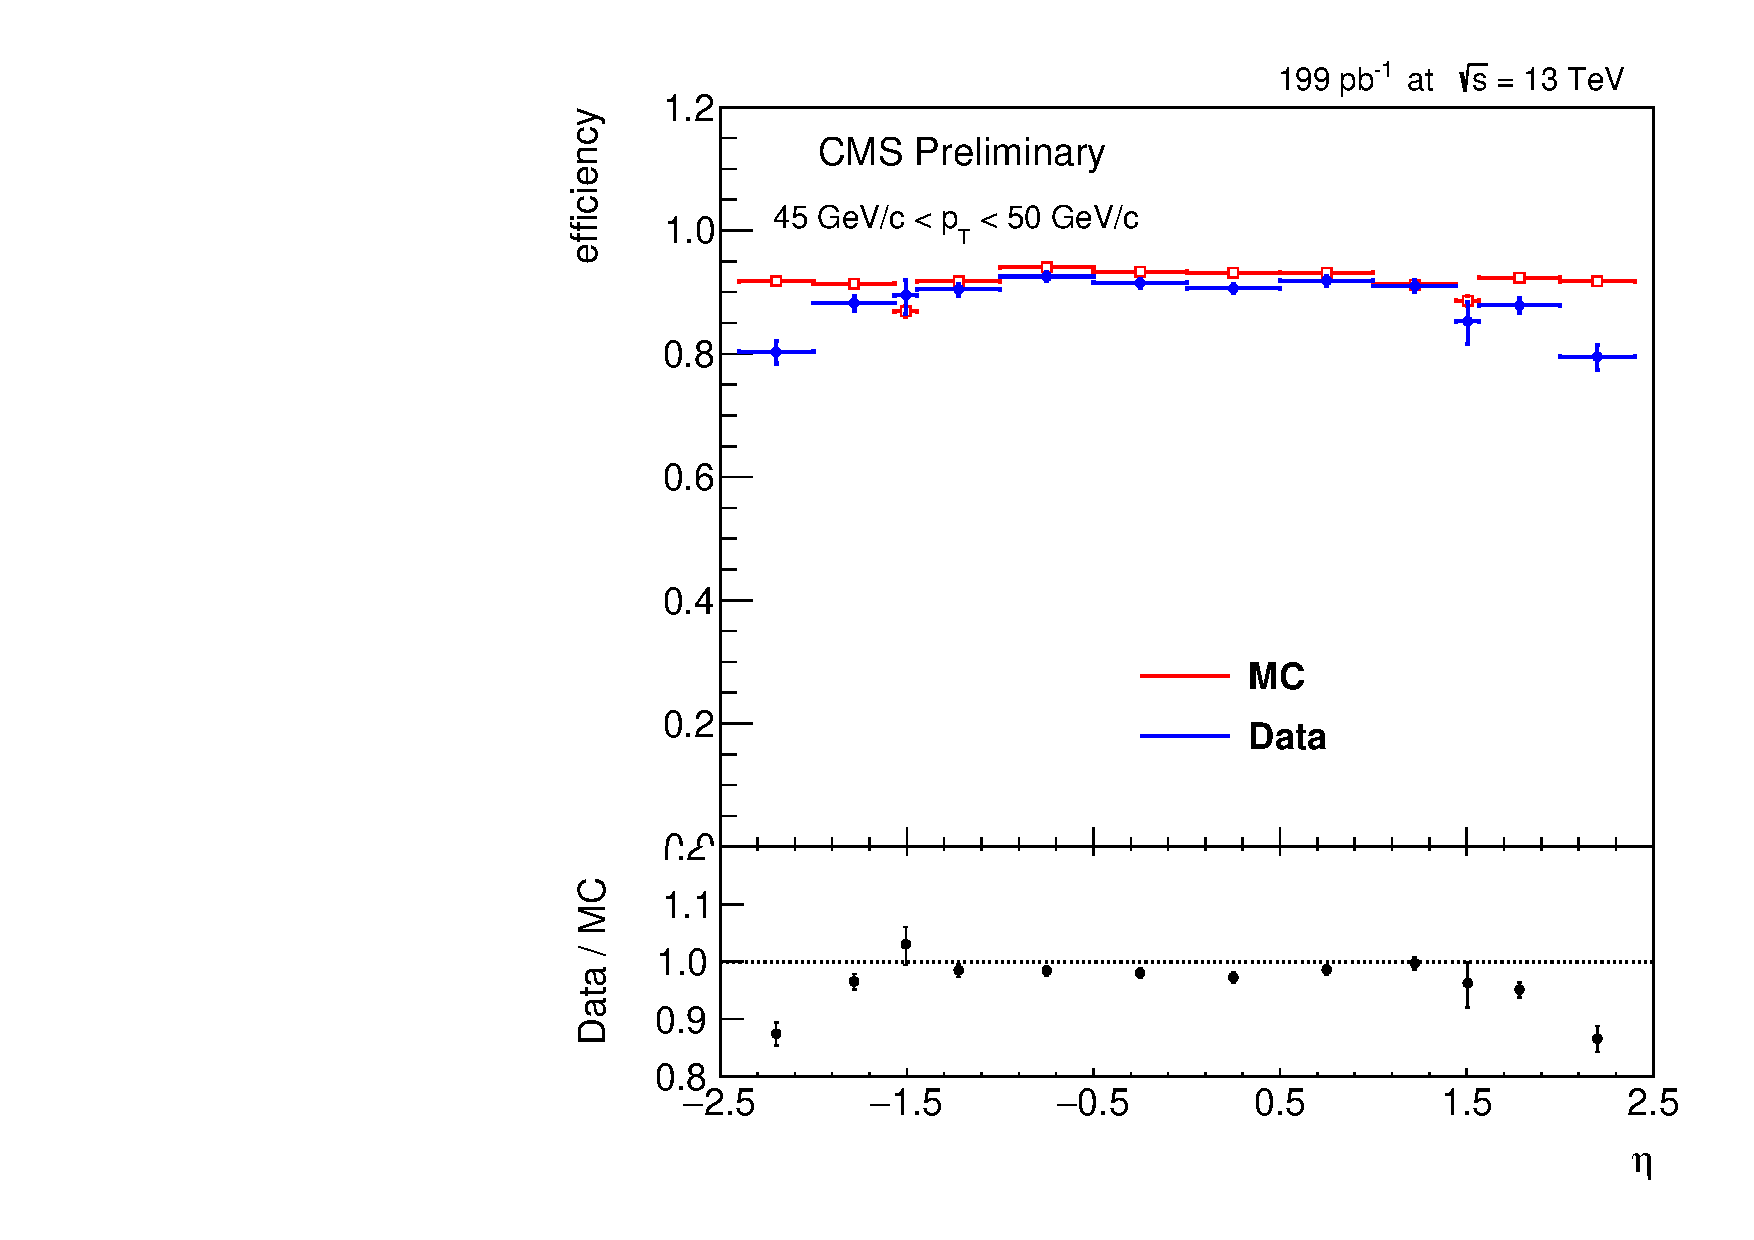
\includegraphics[width=0.45\linewidth]{plots/efficiency/13_zeehlt_positive/PtBins_eta_pt8.pdf}
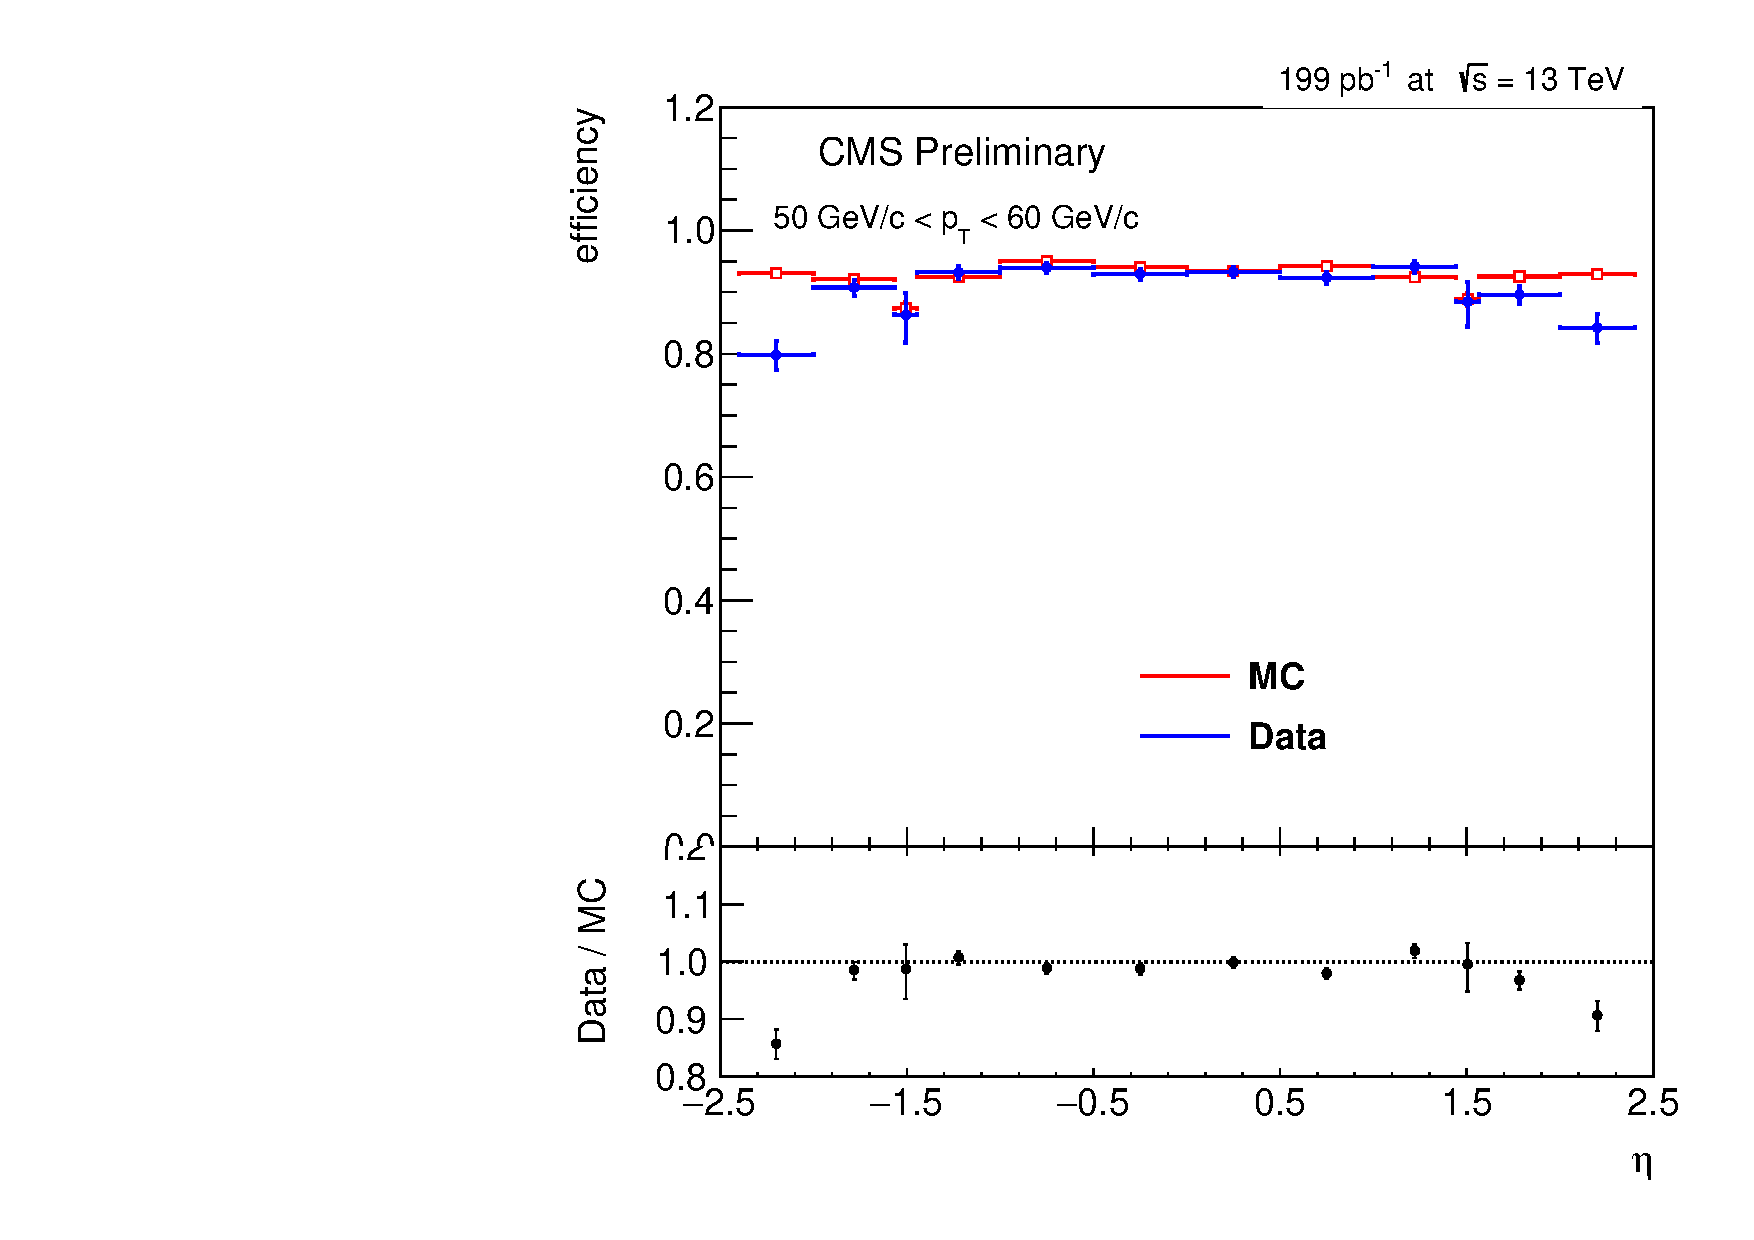
\includegraphics[width=0.45\linewidth]{plots/efficiency/13_zeehlt_positive/PtBins_eta_pt9.pdf}
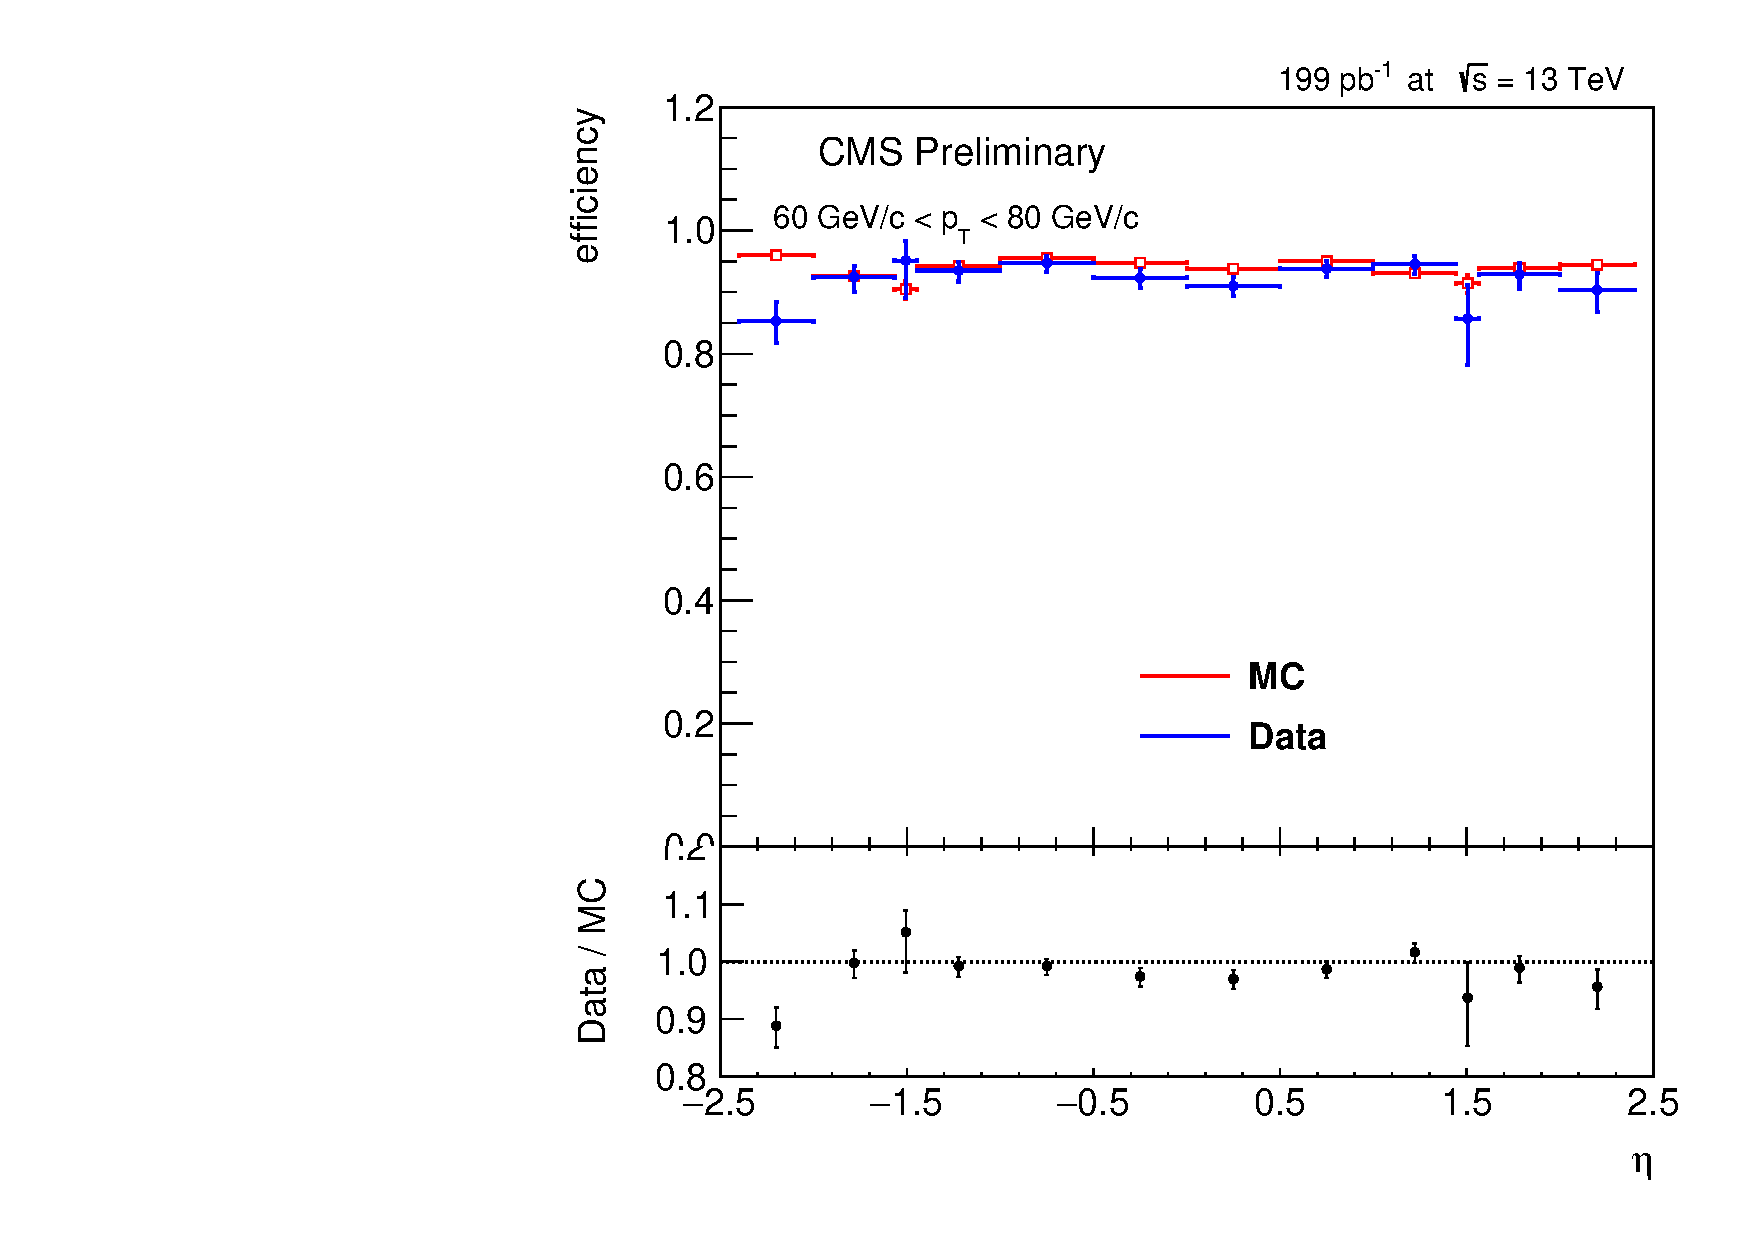
\includegraphics[width=0.45\linewidth]{plots/efficiency/13_zeehlt_positive/PtBins_eta_pt10.pdf}
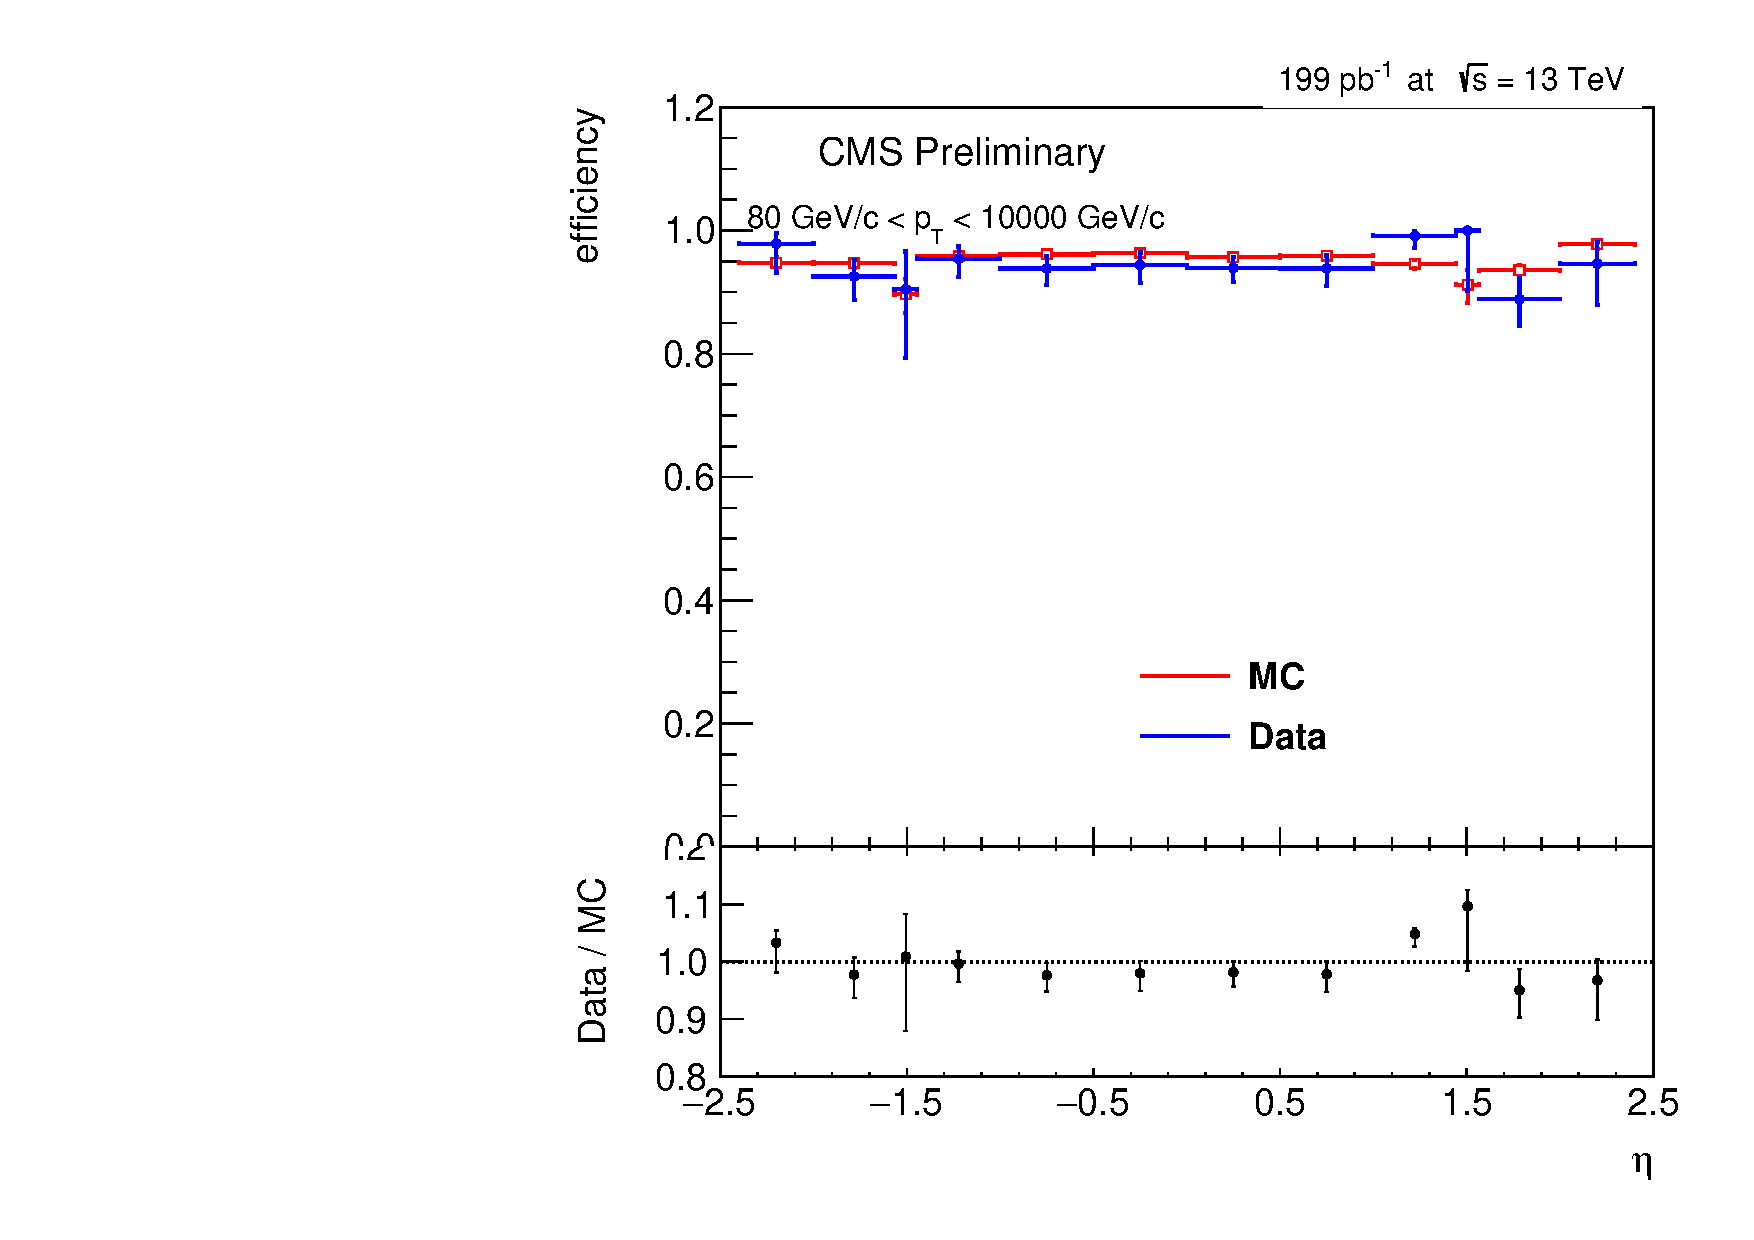
\includegraphics[width=0.45\linewidth]{plots/efficiency/13_zeehlt_positive/PtBins_eta_pt11.pdf}
\caption{$\eta$ dependence of Single electron trigger efficiency scale factors, separated by $p_T$ bins, for positively charged electrons in the 13 TeV samples.}
\label{fig:Eff:el:13:HLT:pos}
\end{figure}
\begin{figure}
\centering
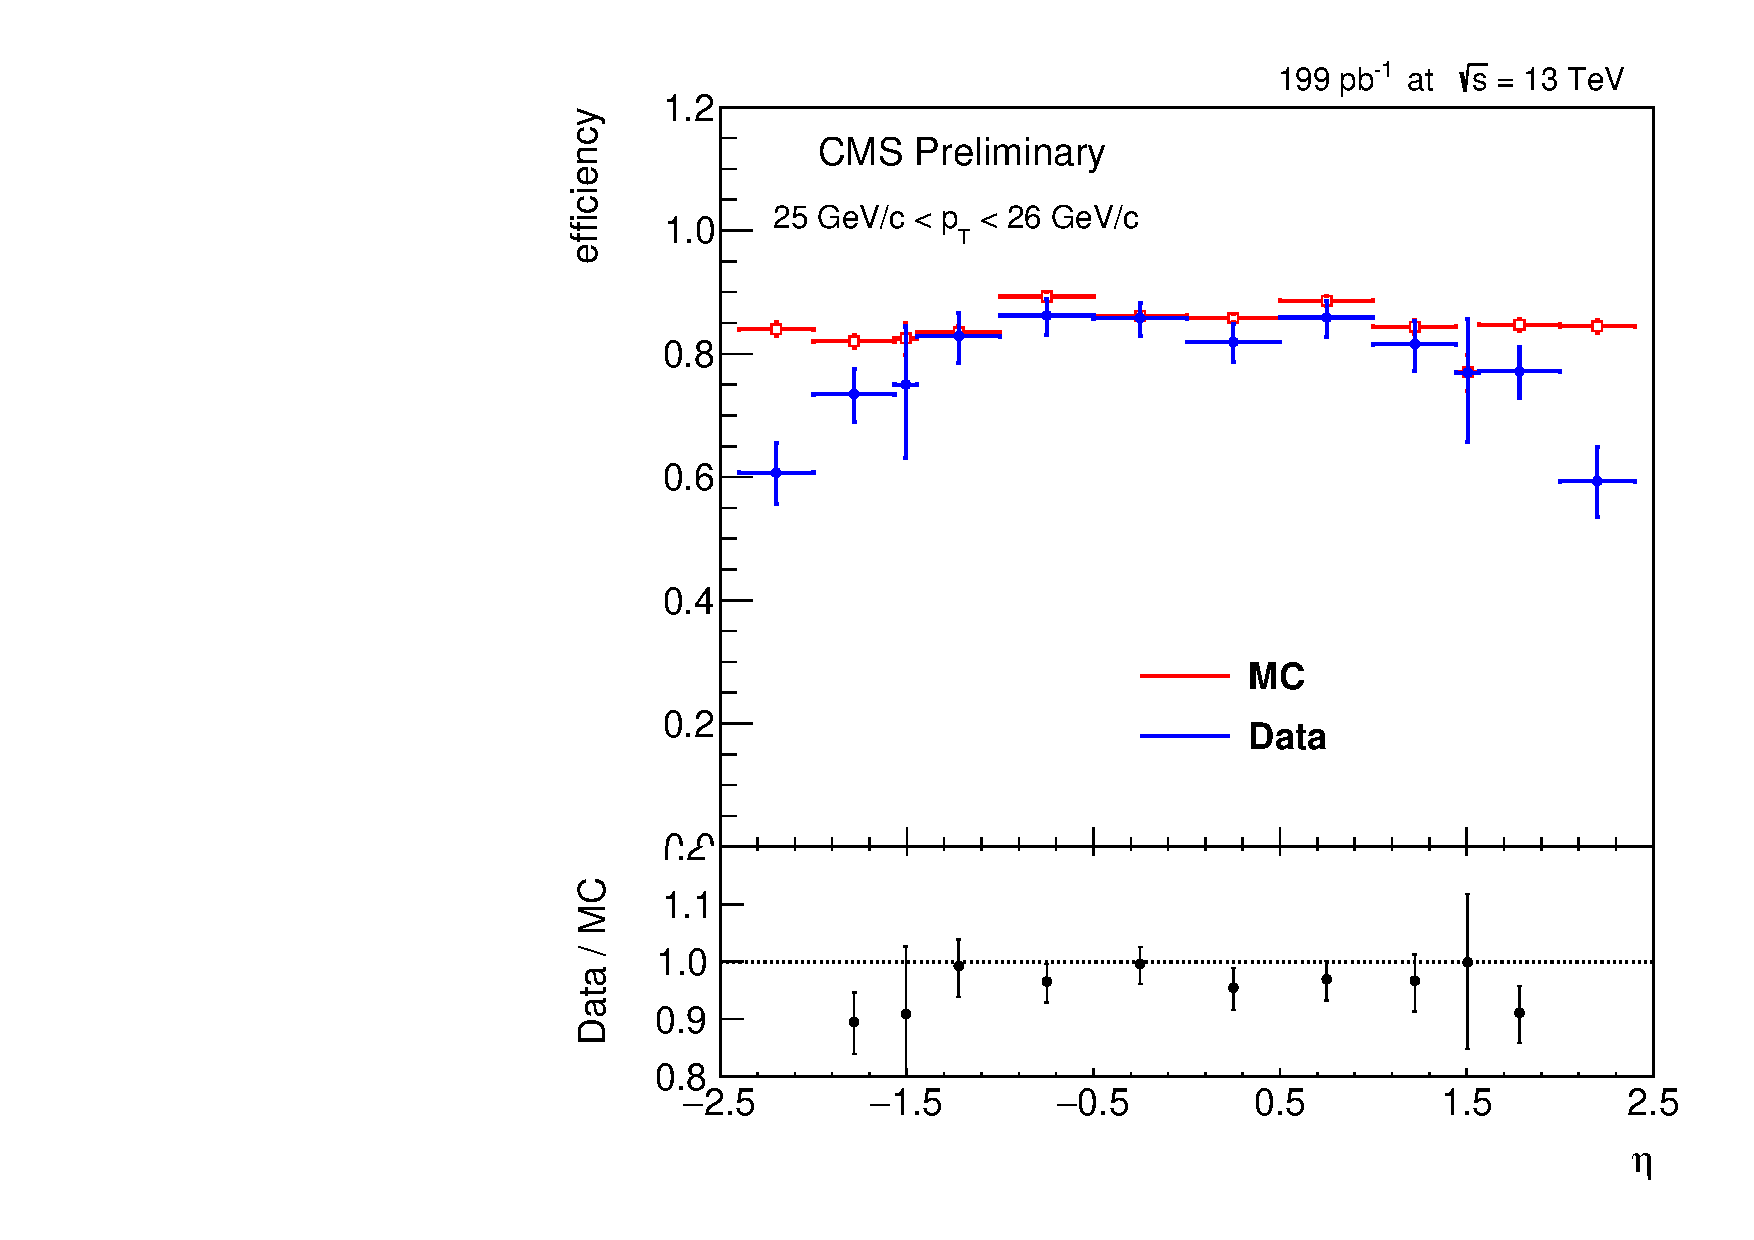
\includegraphics[width=0.45\linewidth]{plots/efficiency/13_zeehlt_negative/PtBins_eta_pt0.pdf}
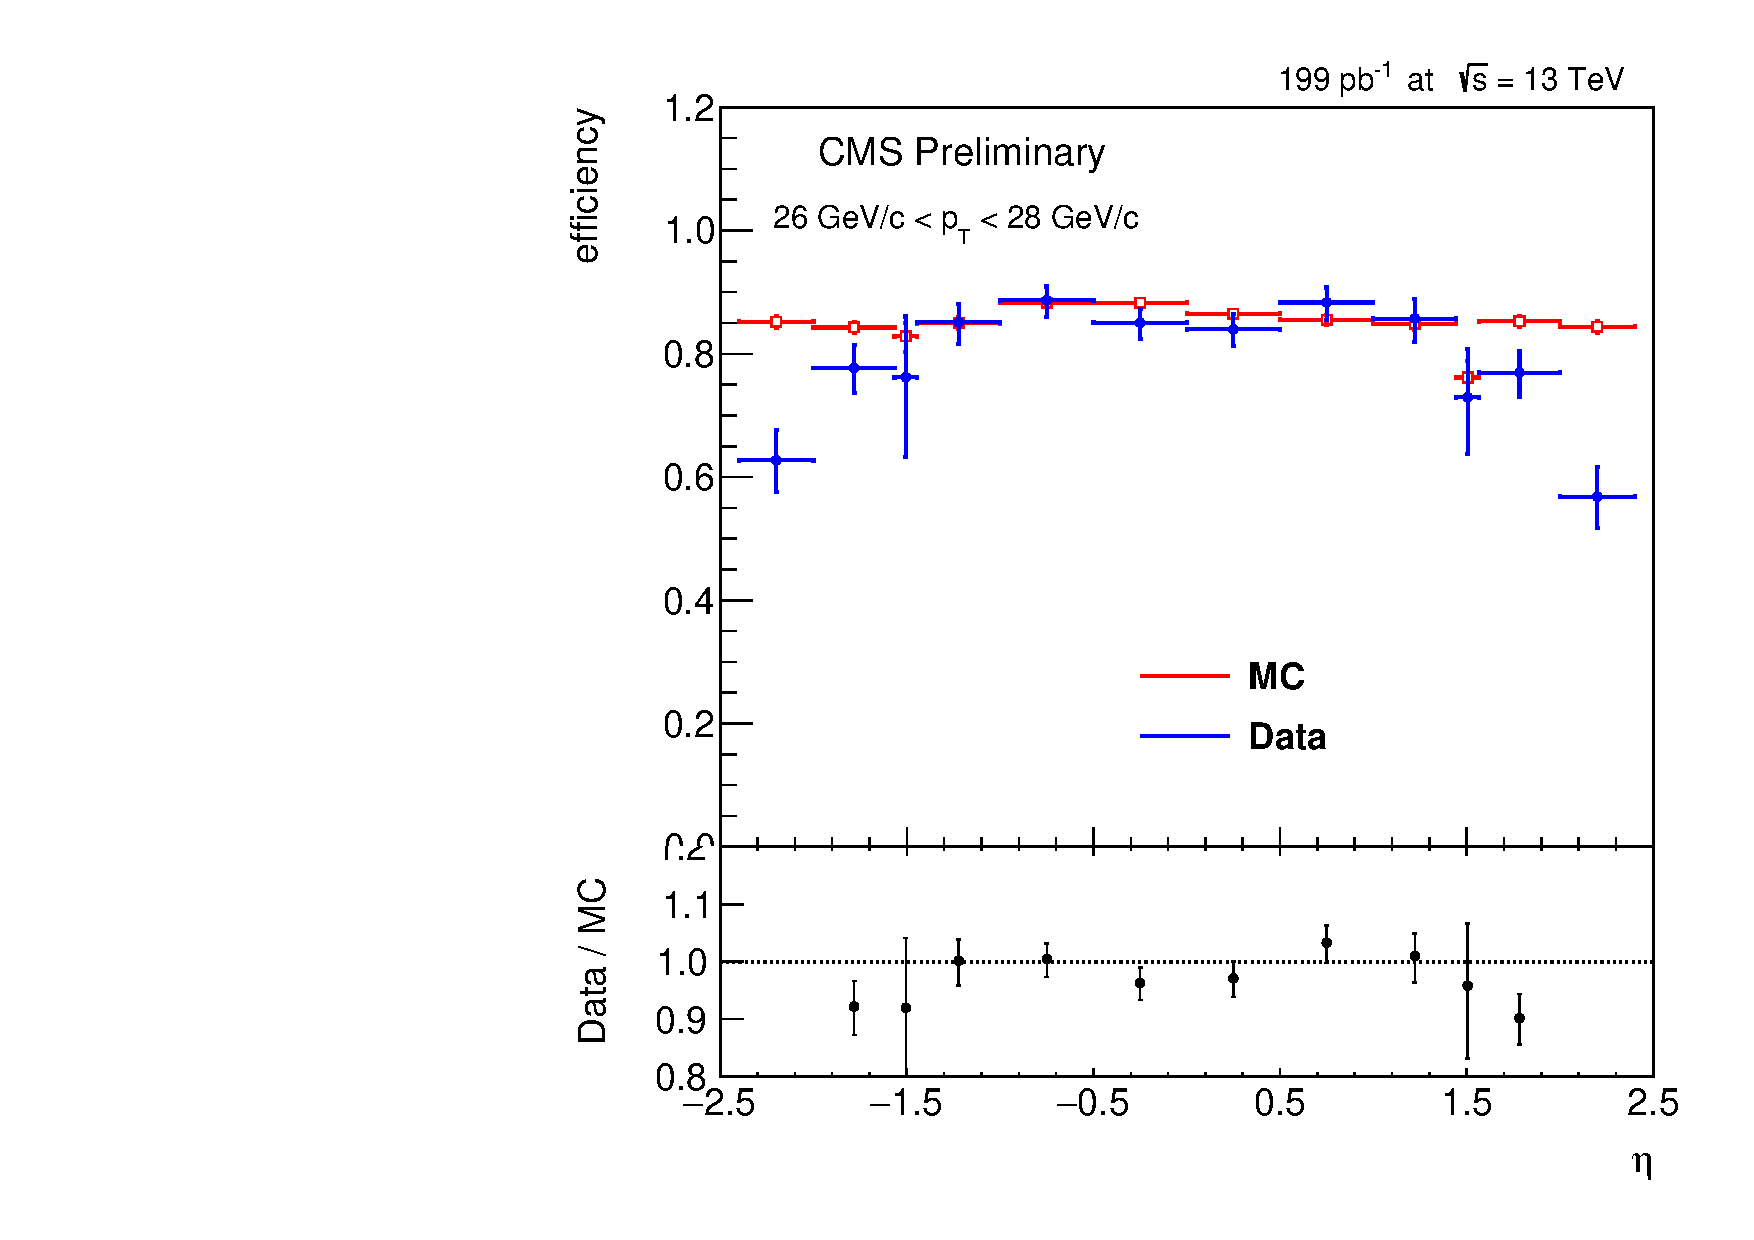
\includegraphics[width=0.45\linewidth]{plots/efficiency/13_zeehlt_negative/PtBins_eta_pt1.pdf}
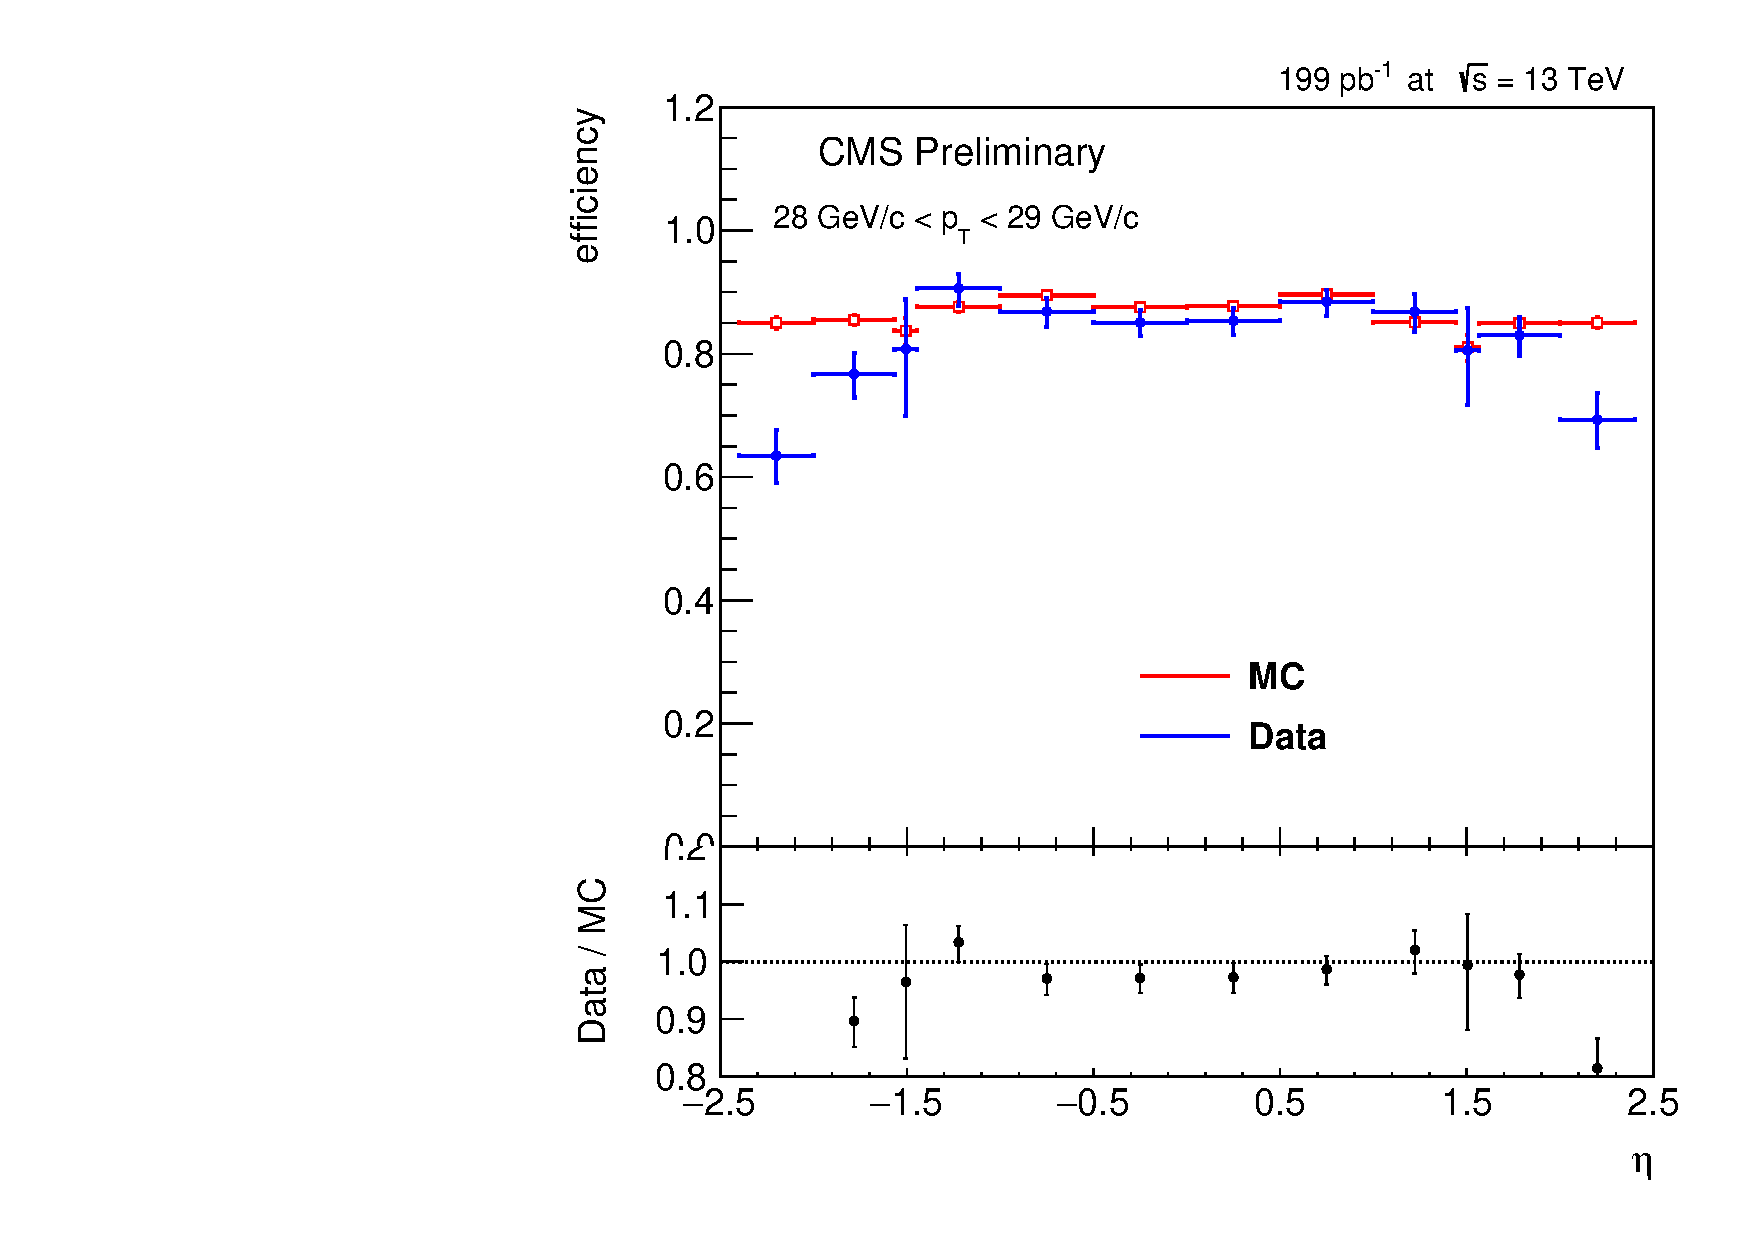
\includegraphics[width=0.45\linewidth]{plots/efficiency/13_zeehlt_negative/PtBins_eta_pt2.pdf}
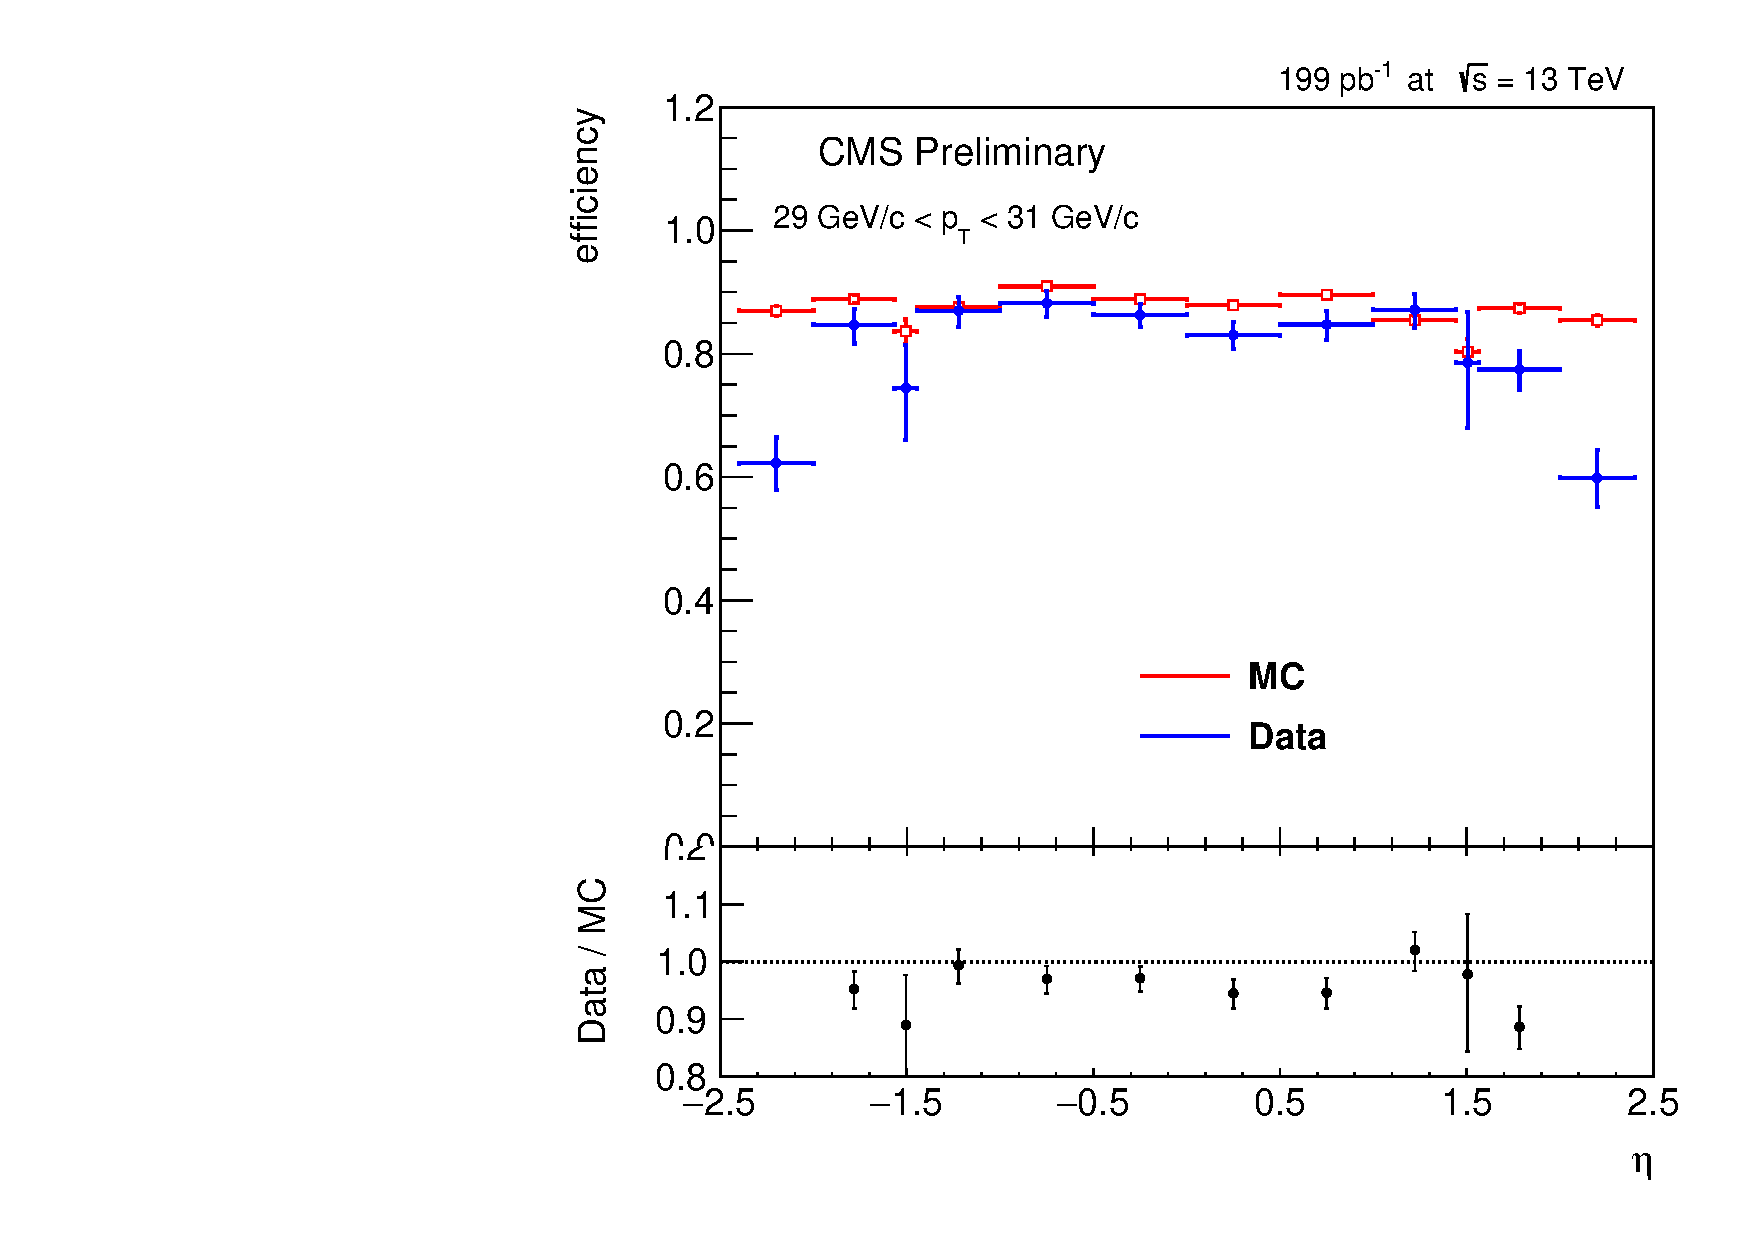
\includegraphics[width=0.45\linewidth]{plots/efficiency/13_zeehlt_negative/PtBins_eta_pt3.pdf}
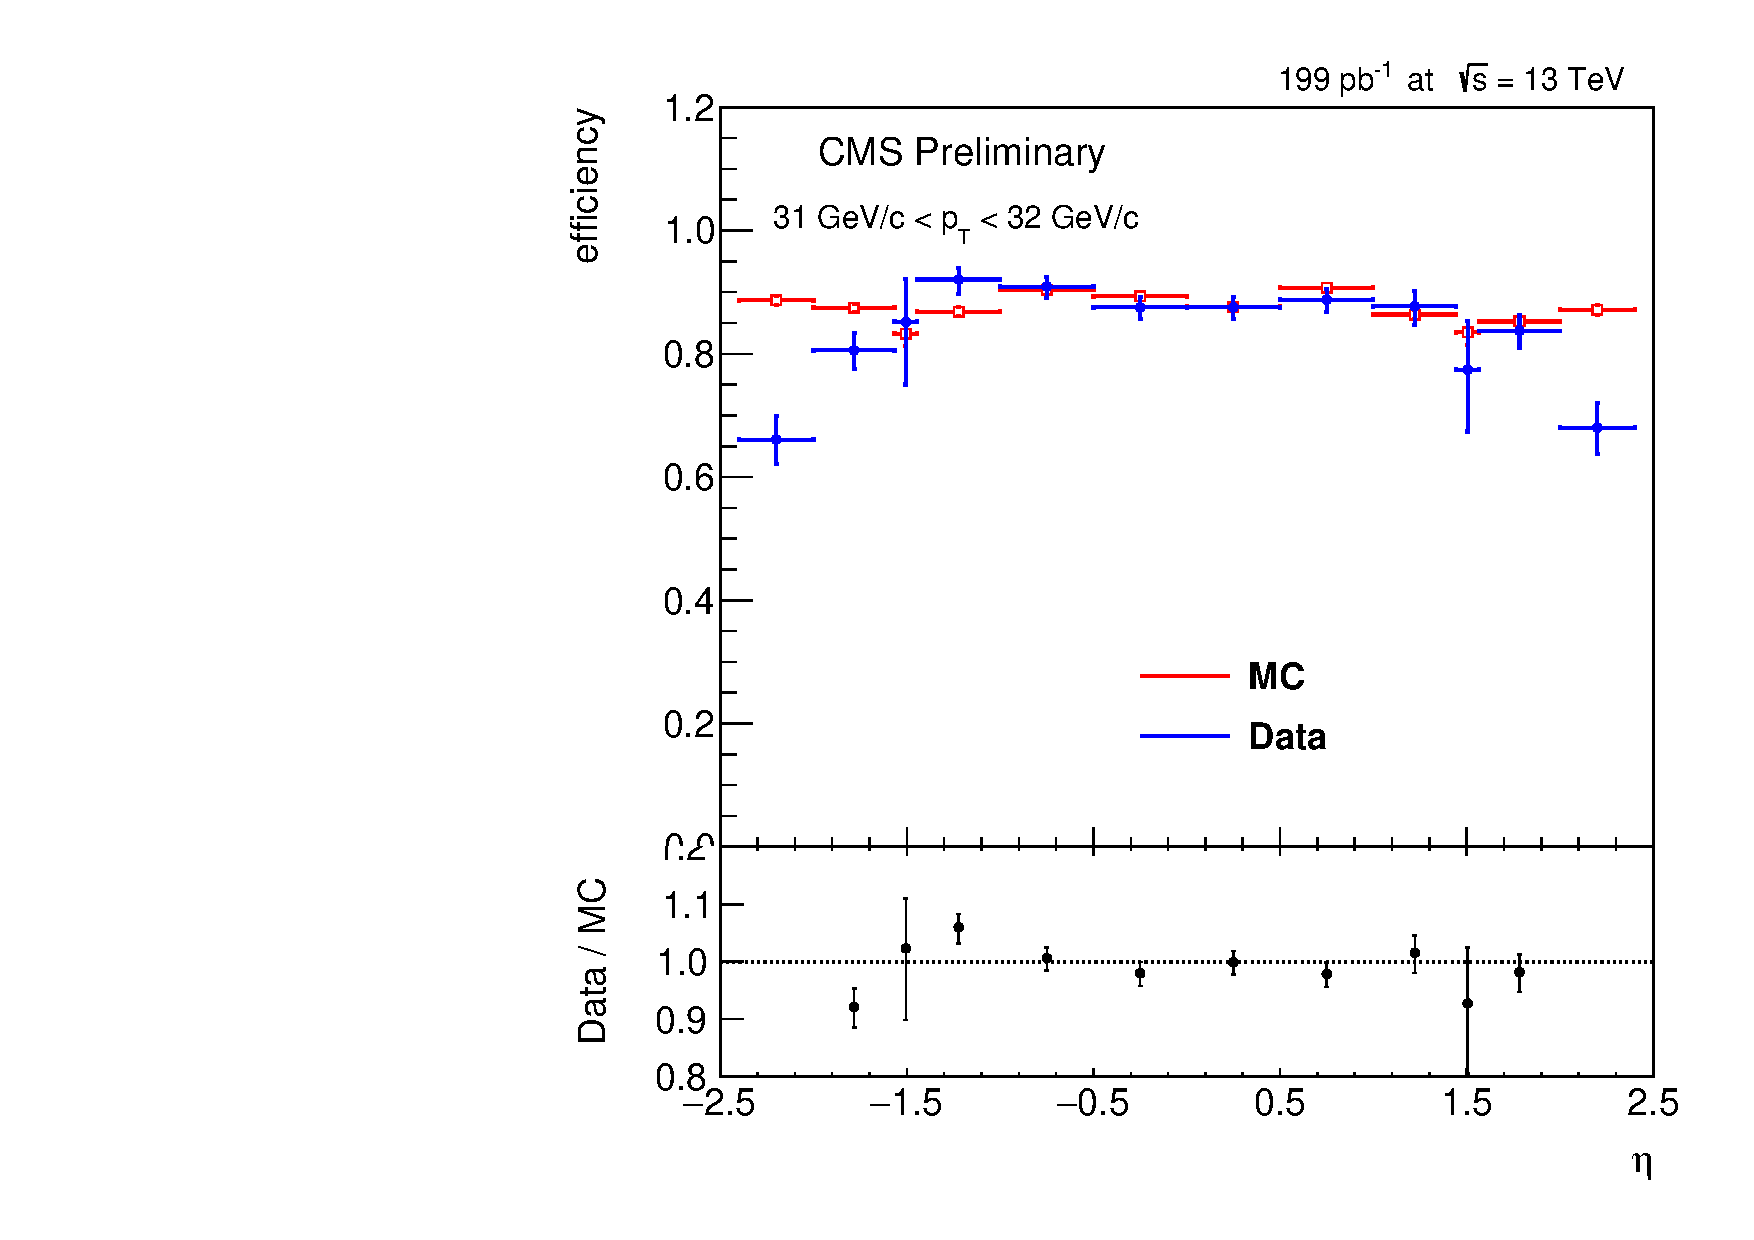
\includegraphics[width=0.45\linewidth]{plots/efficiency/13_zeehlt_negative/PtBins_eta_pt4.pdf}
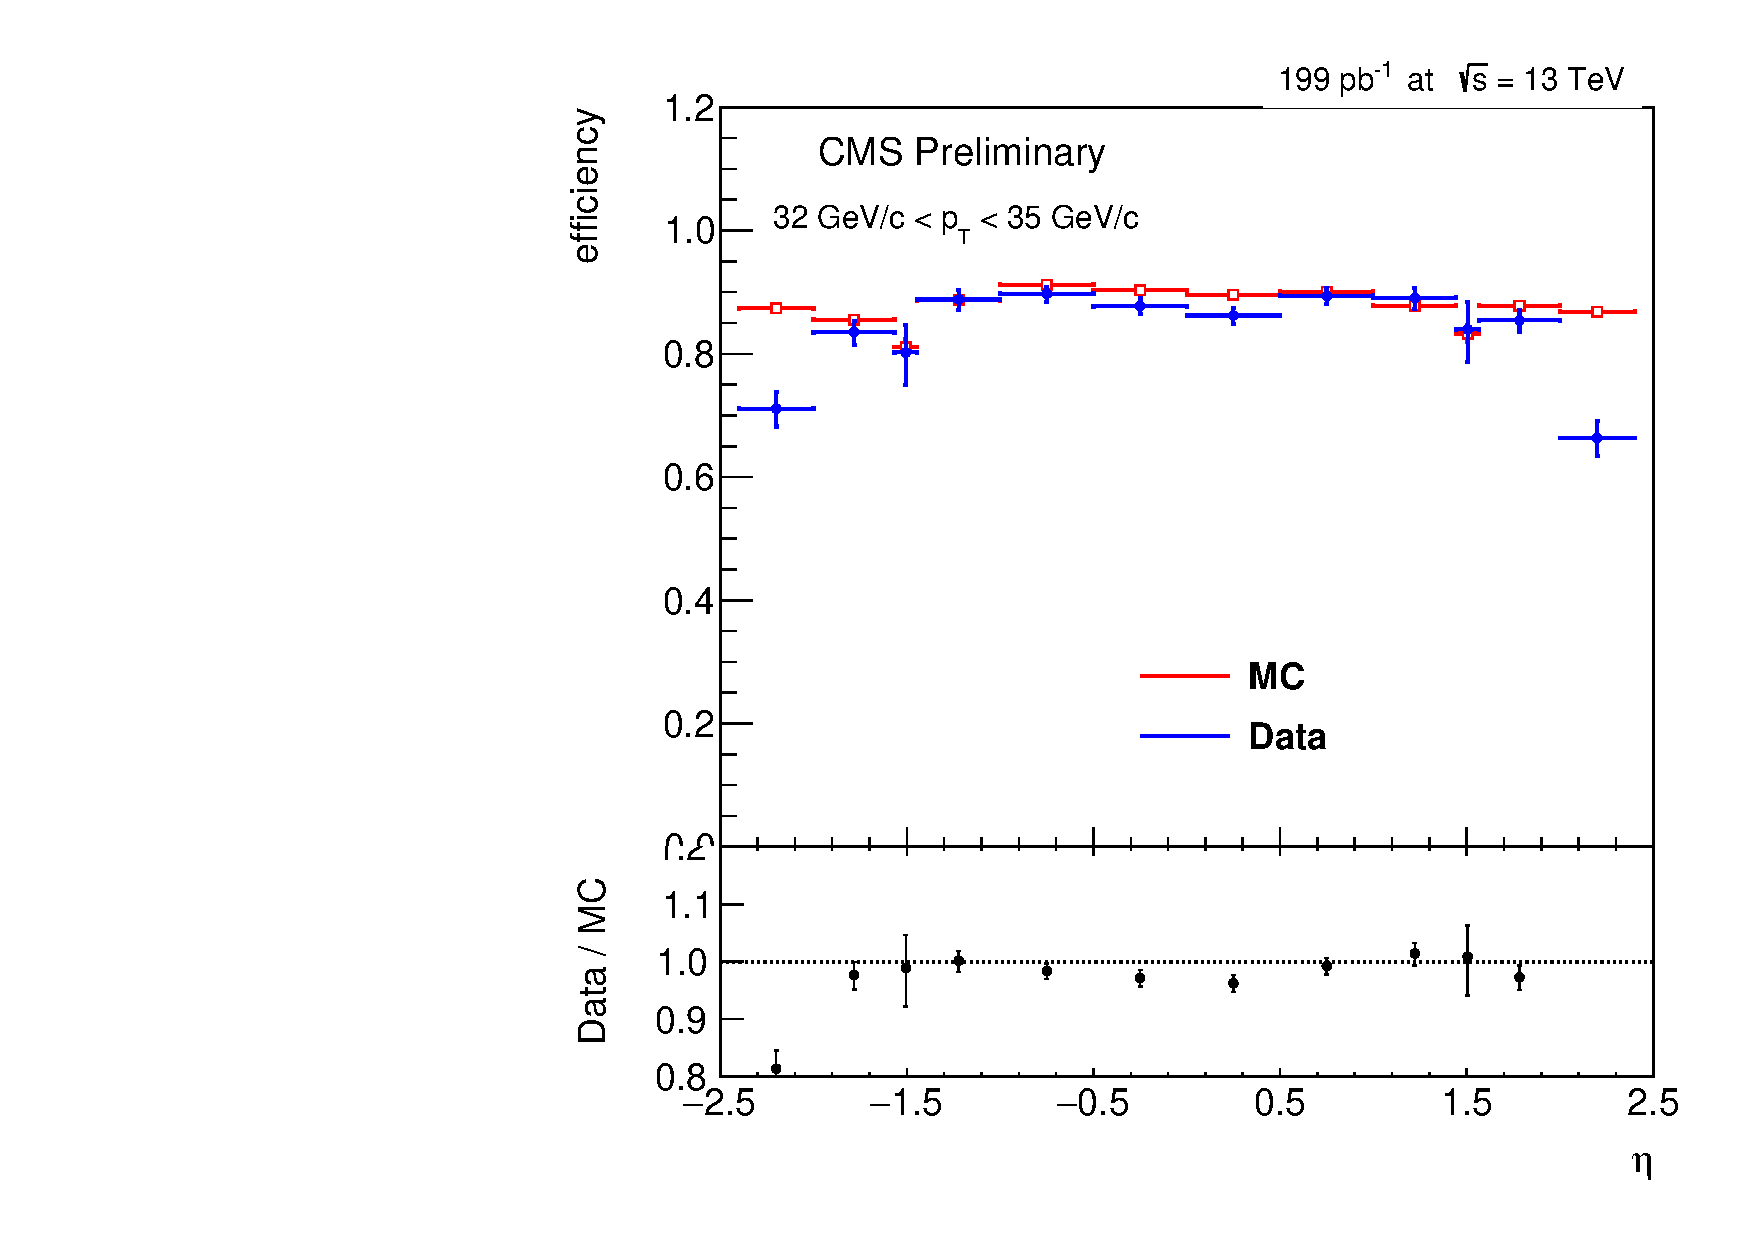
\includegraphics[width=0.45\linewidth]{plots/efficiency/13_zeehlt_negative/PtBins_eta_pt5.pdf}
\caption{$\eta$ dependence of Single electron trigger efficiency scale factors, separated by $p_T$ bins, for negatively charged electrons in the 13 TeV samples.}
% \label{fig:Eff:el:13:HLT:neg}
\end{figure}
\begin{figure}
\ContinuedFloat
\centering
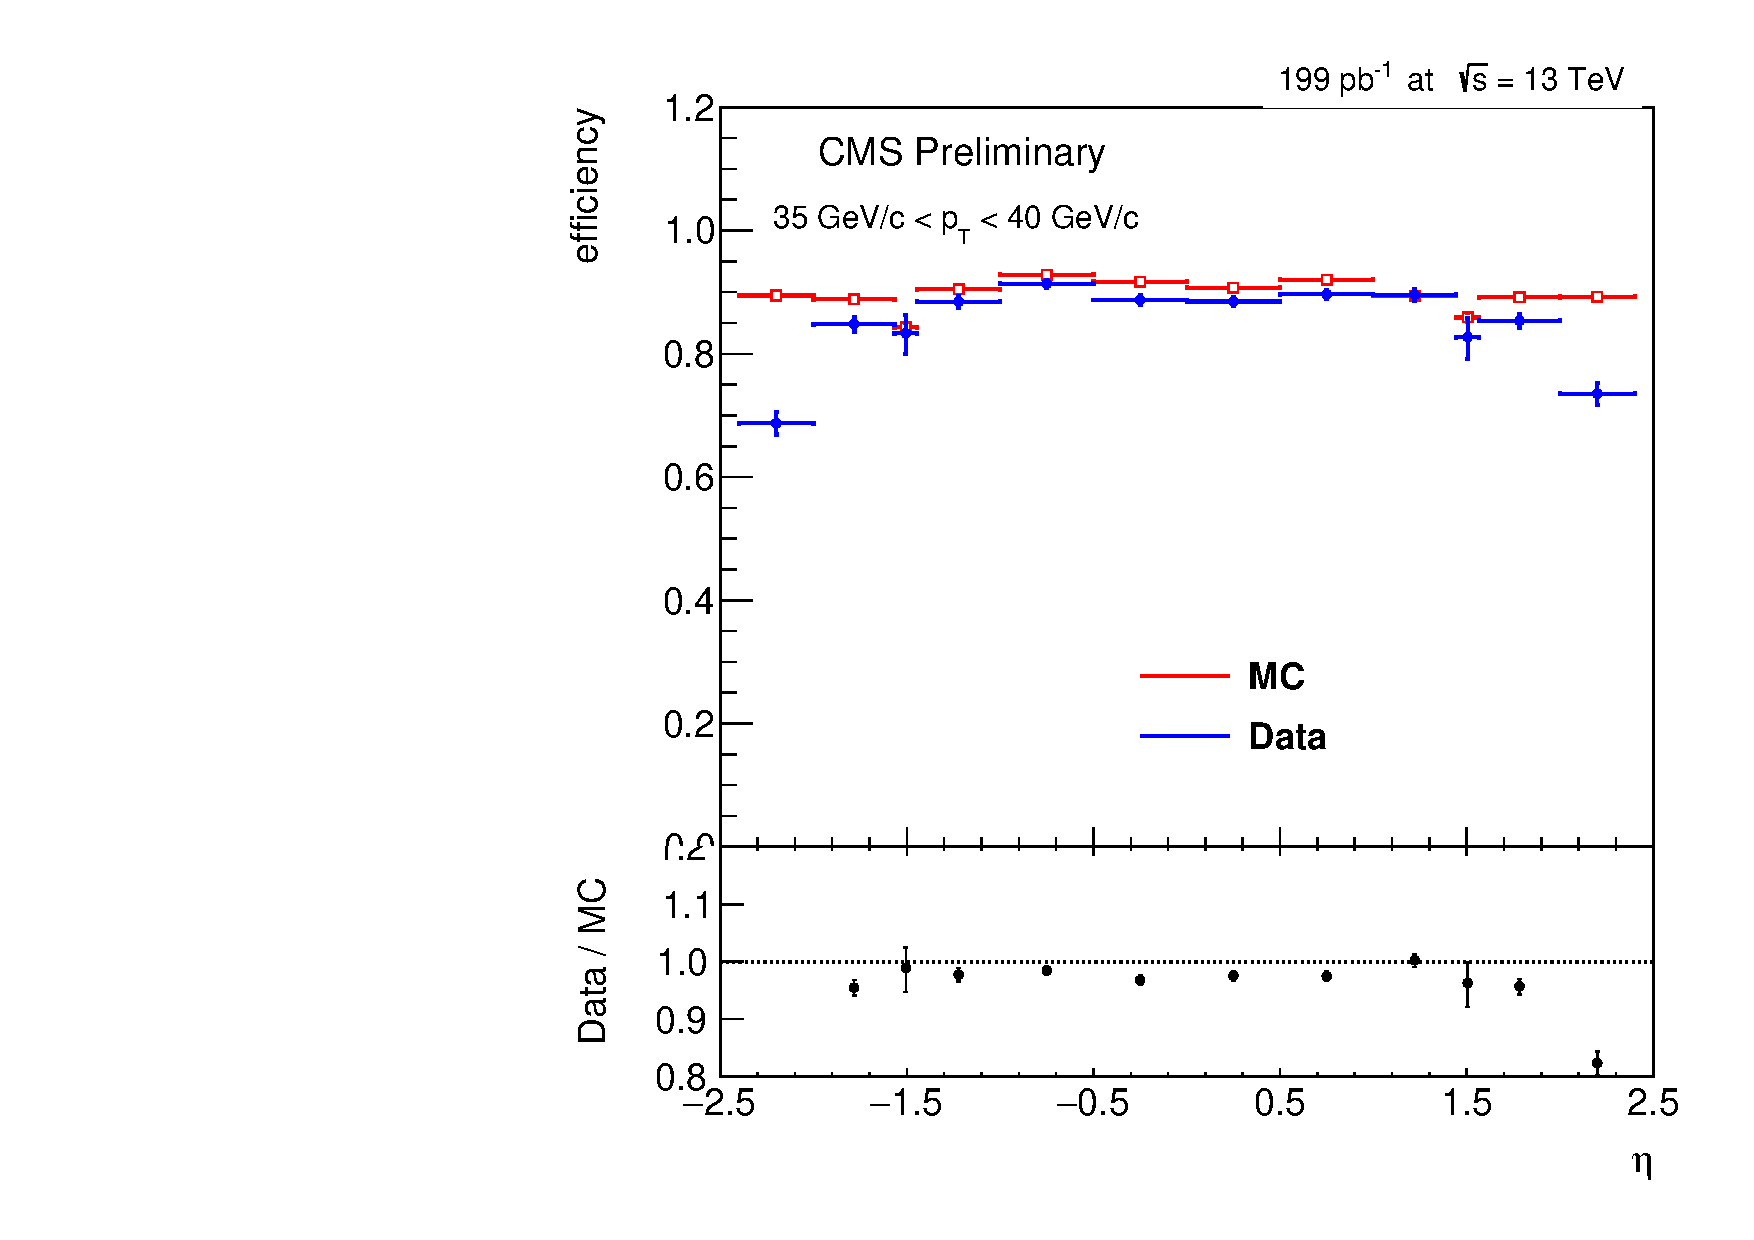
\includegraphics[width=0.45\linewidth]{plots/efficiency/13_zeehlt_negative/PtBins_eta_pt6.pdf}
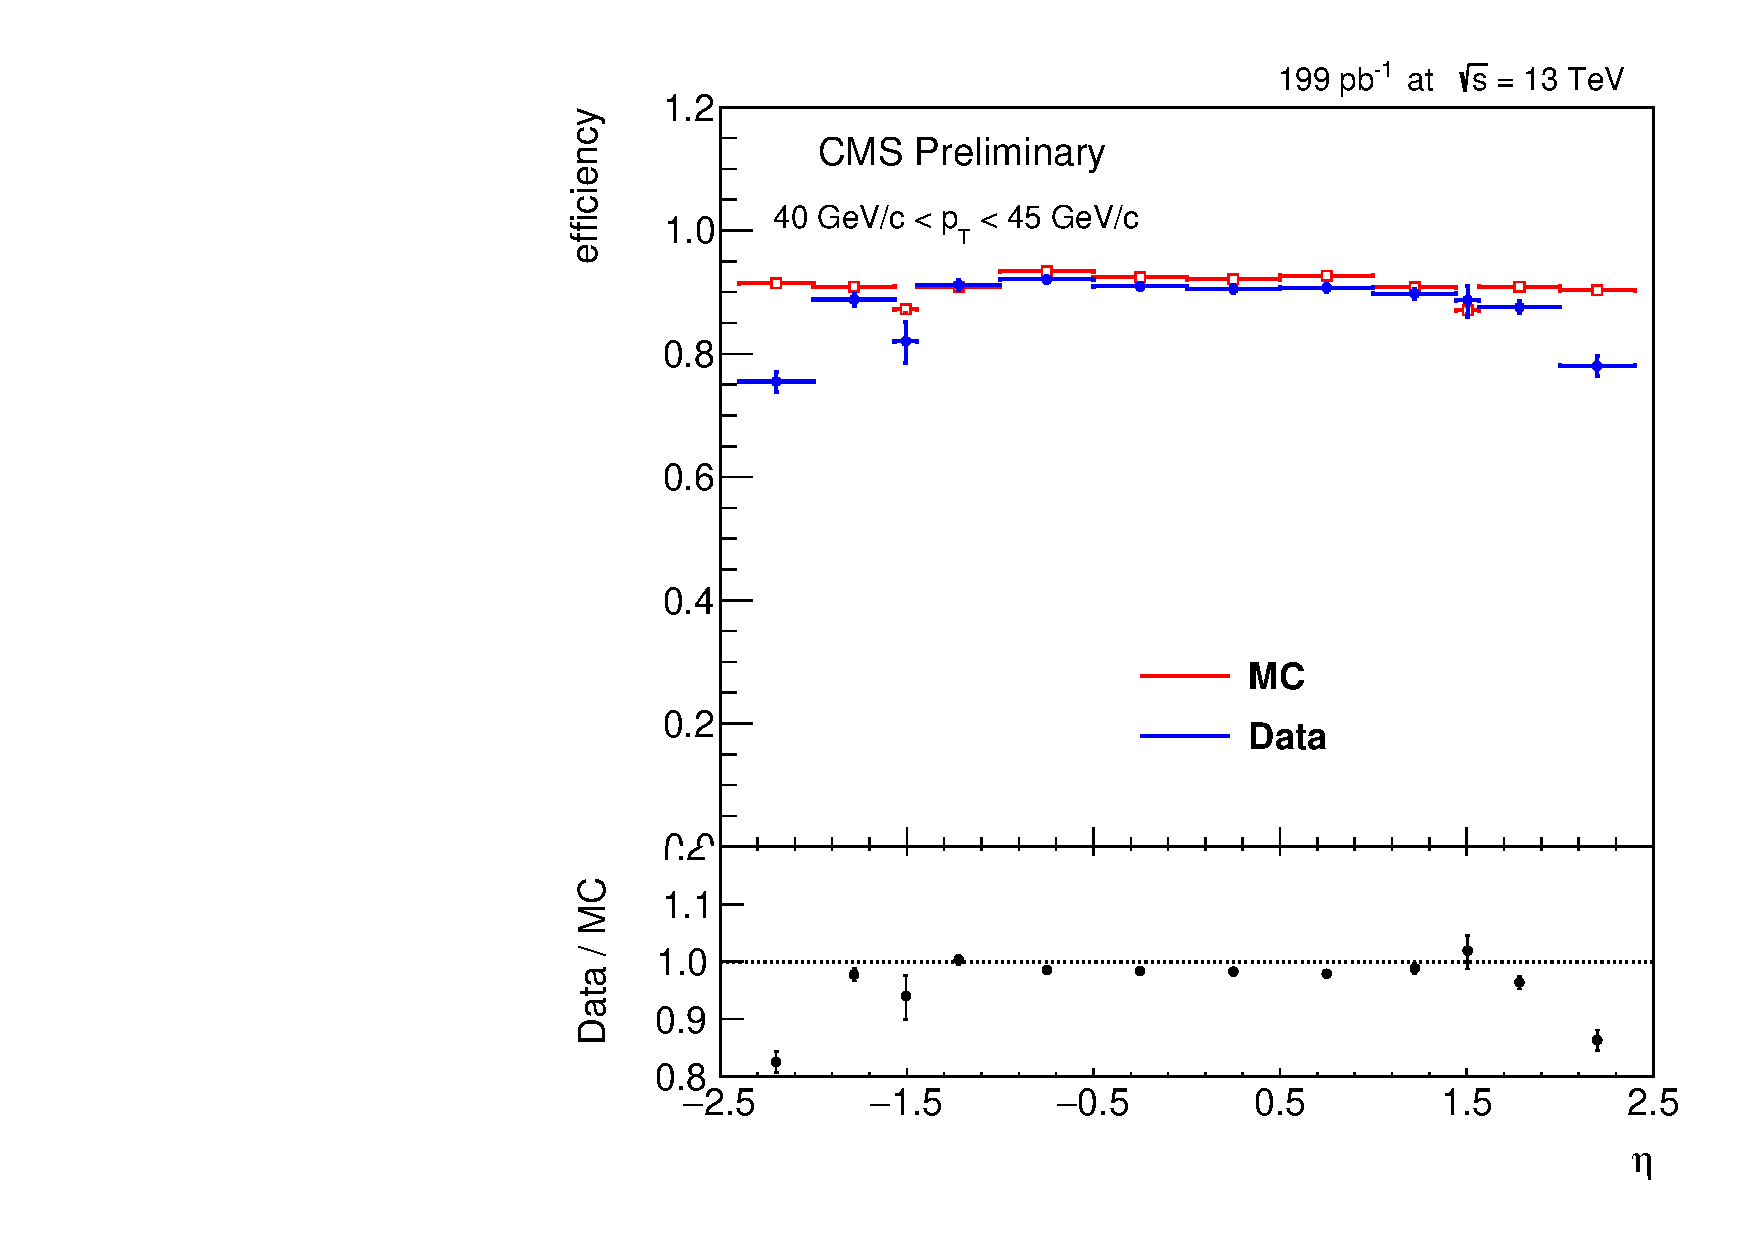
\includegraphics[width=0.45\linewidth]{plots/efficiency/13_zeehlt_negative/PtBins_eta_pt7.pdf}
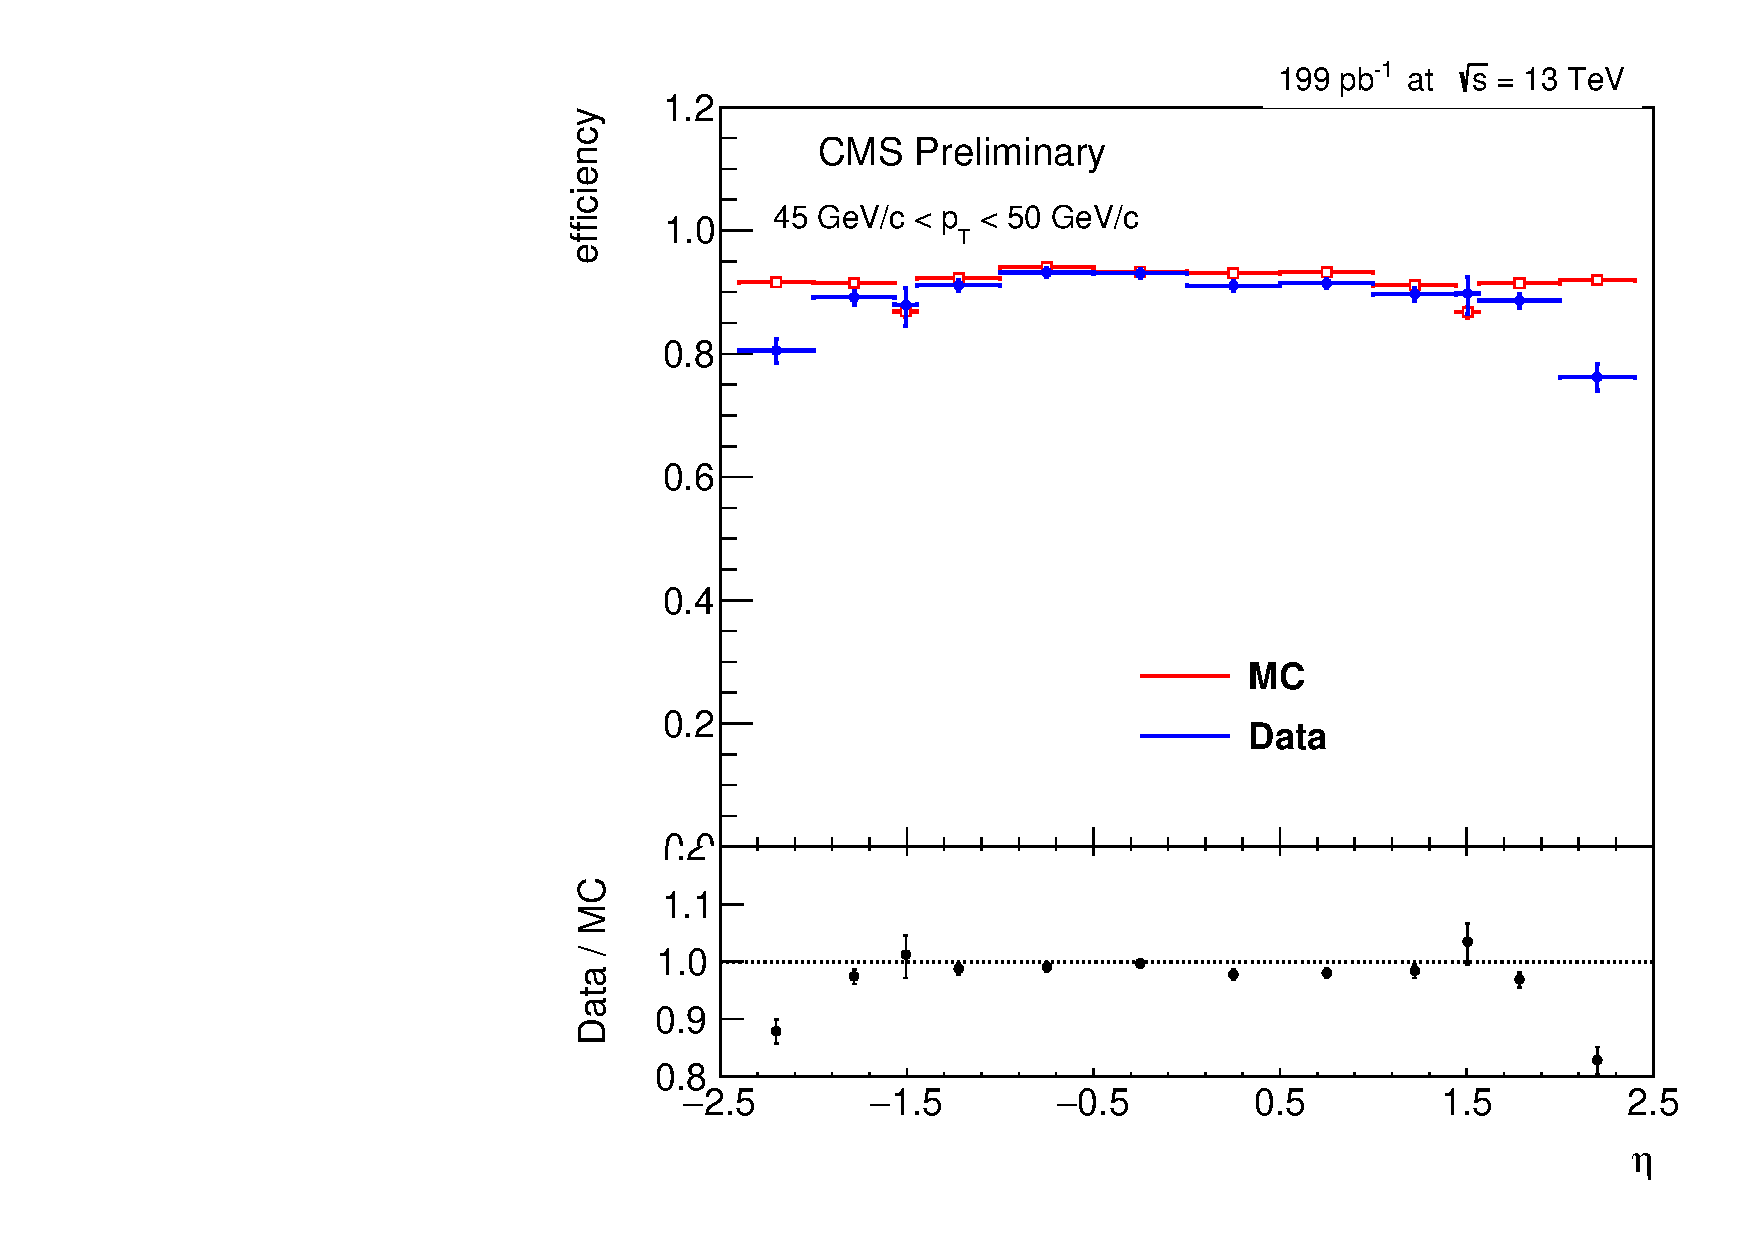
\includegraphics[width=0.45\linewidth]{plots/efficiency/13_zeehlt_negative/PtBins_eta_pt8.pdf}
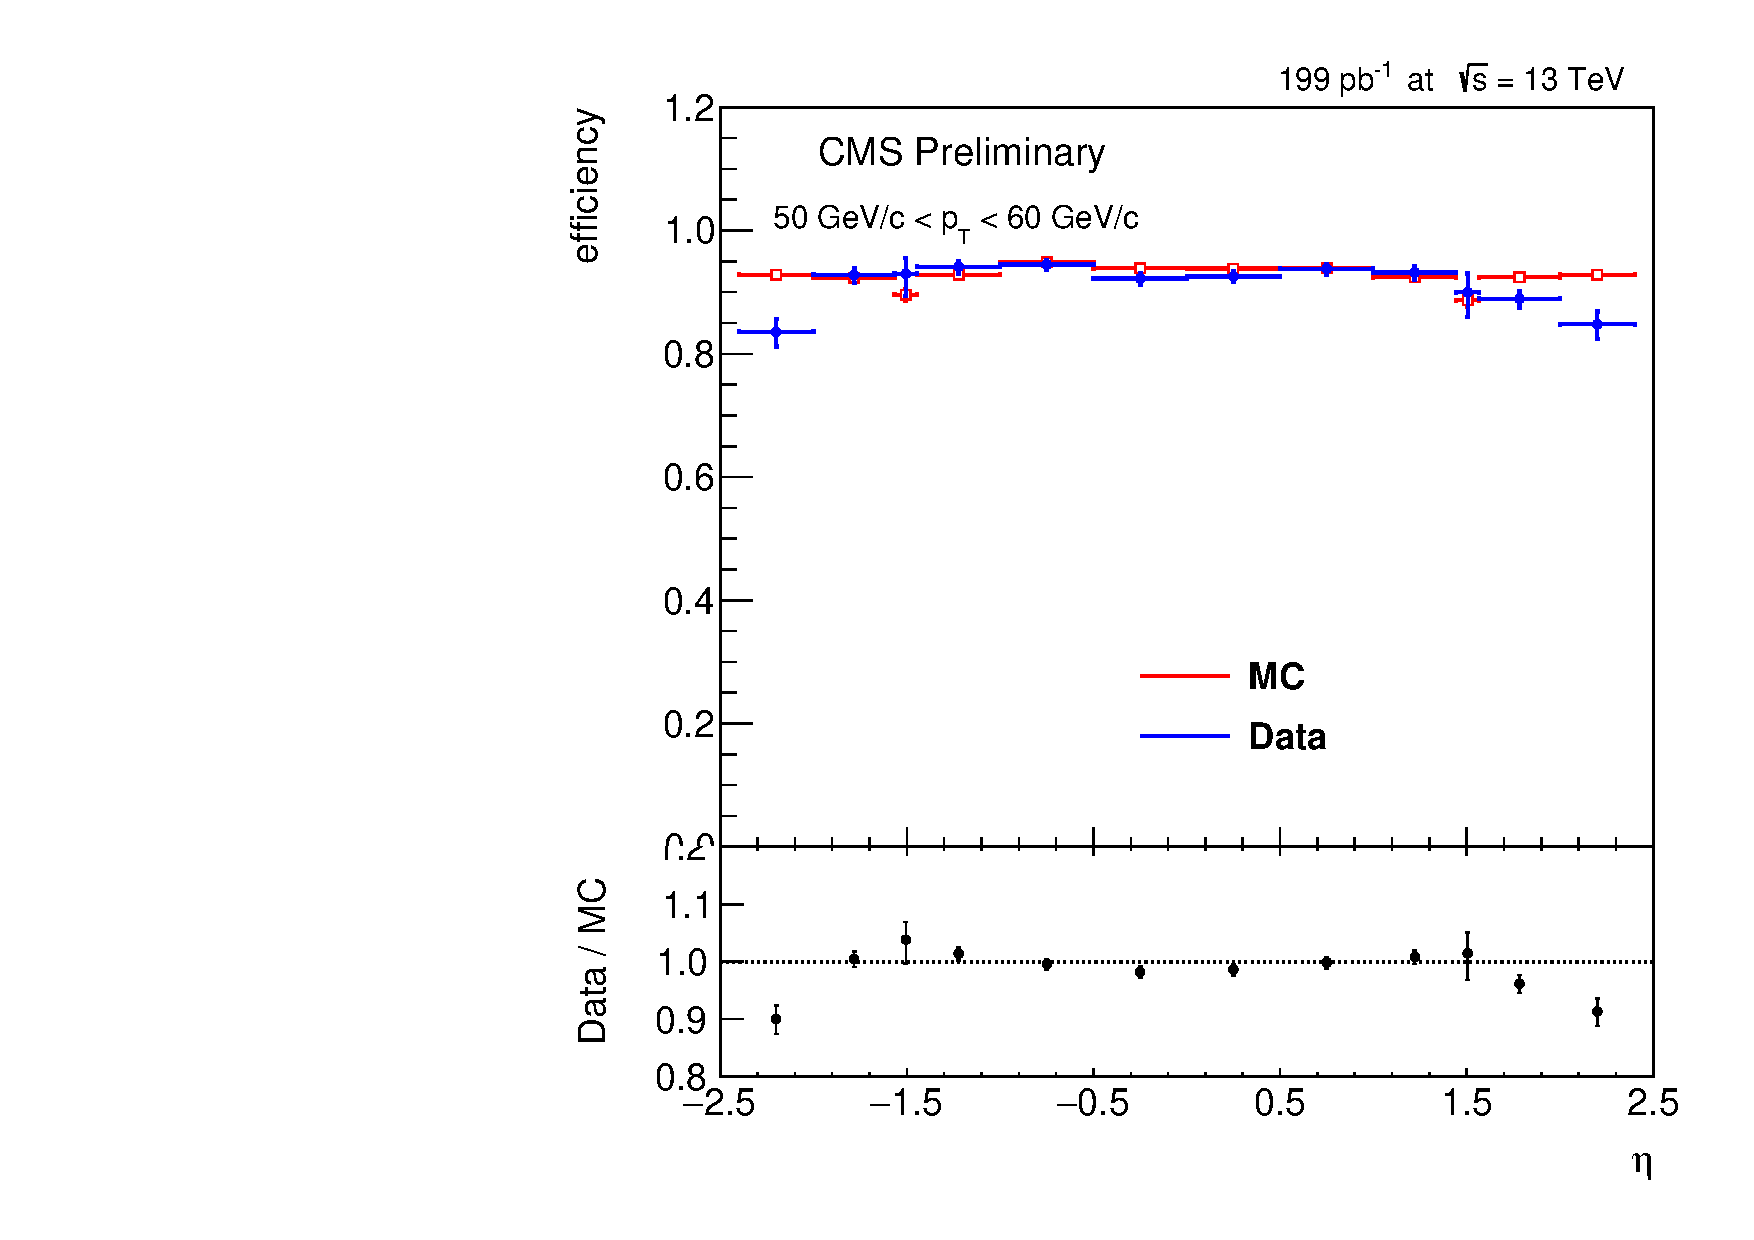
\includegraphics[width=0.45\linewidth]{plots/efficiency/13_zeehlt_negative/PtBins_eta_pt9.pdf}
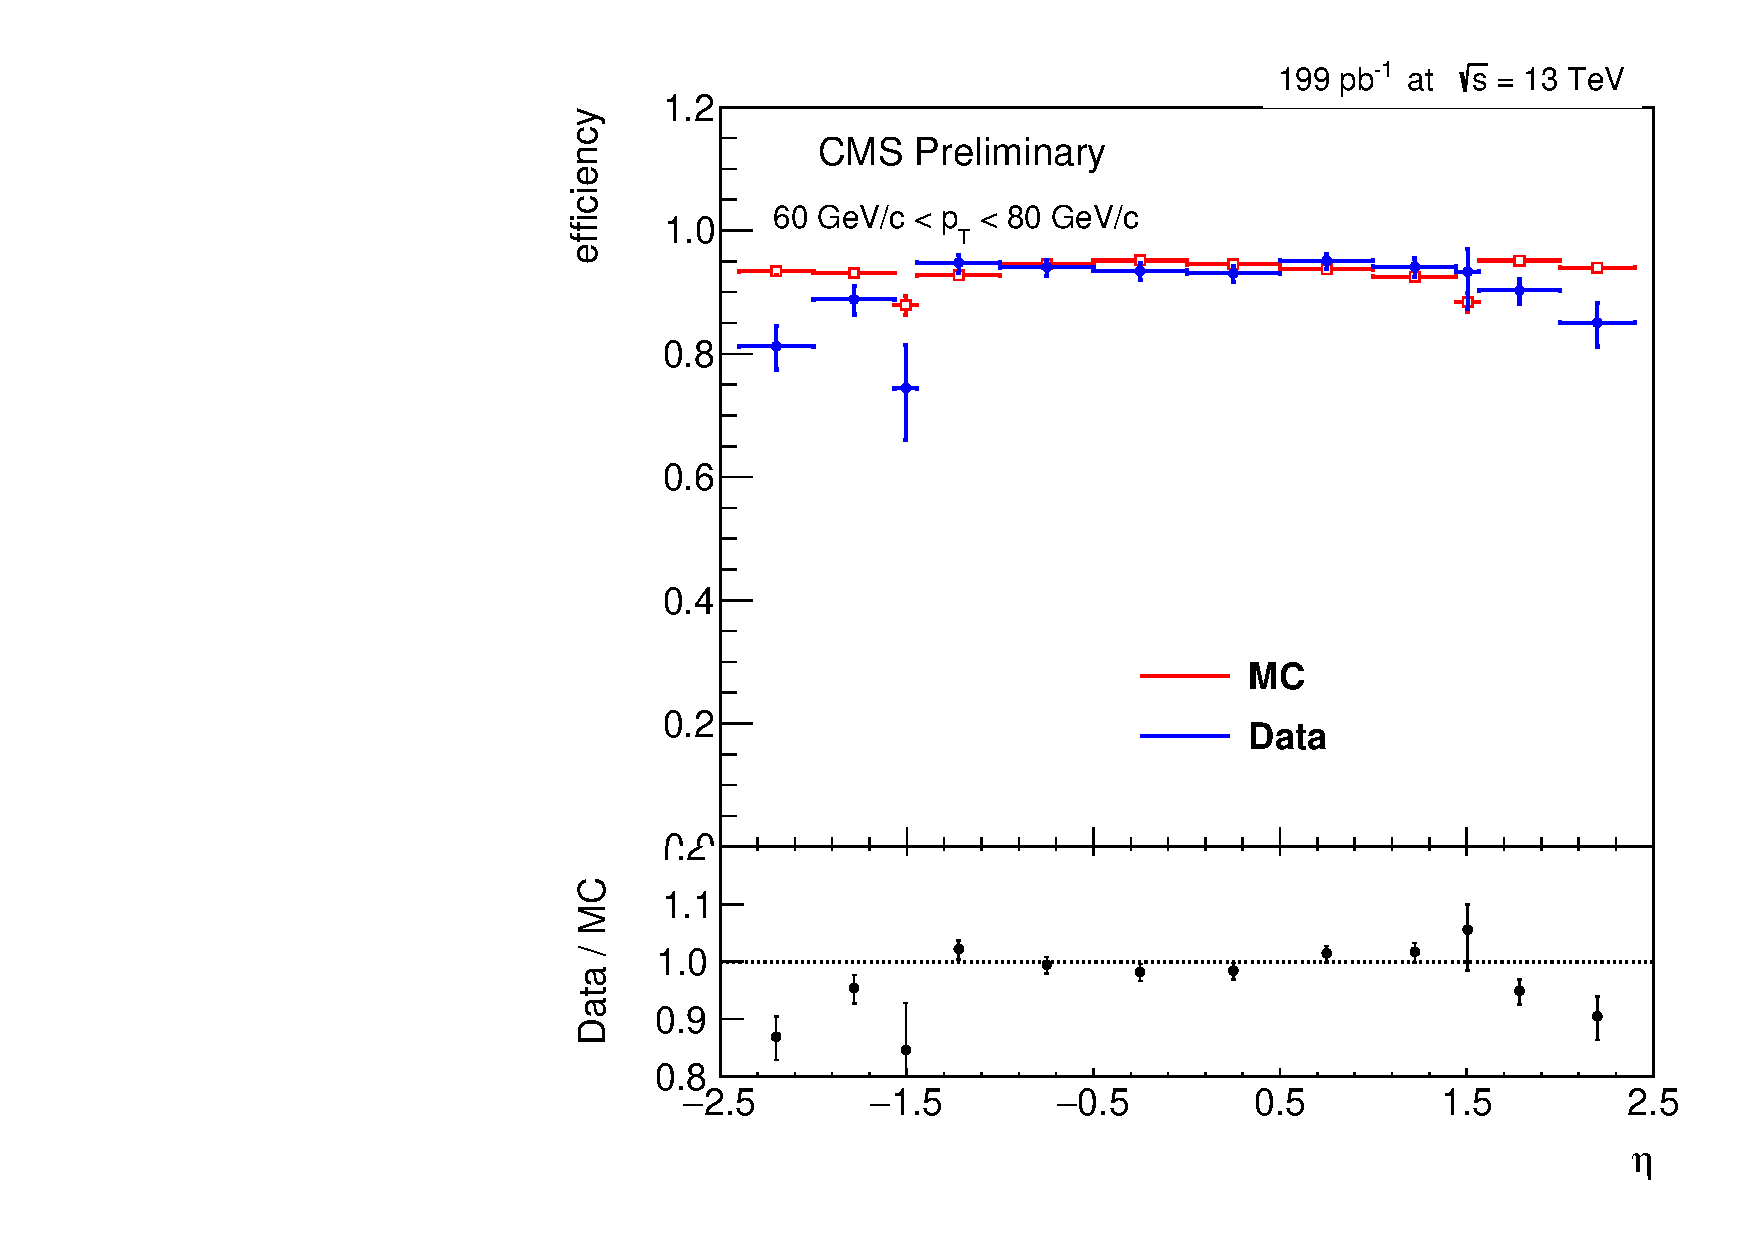
\includegraphics[width=0.45\linewidth]{plots/efficiency/13_zeehlt_negative/PtBins_eta_pt10.pdf}
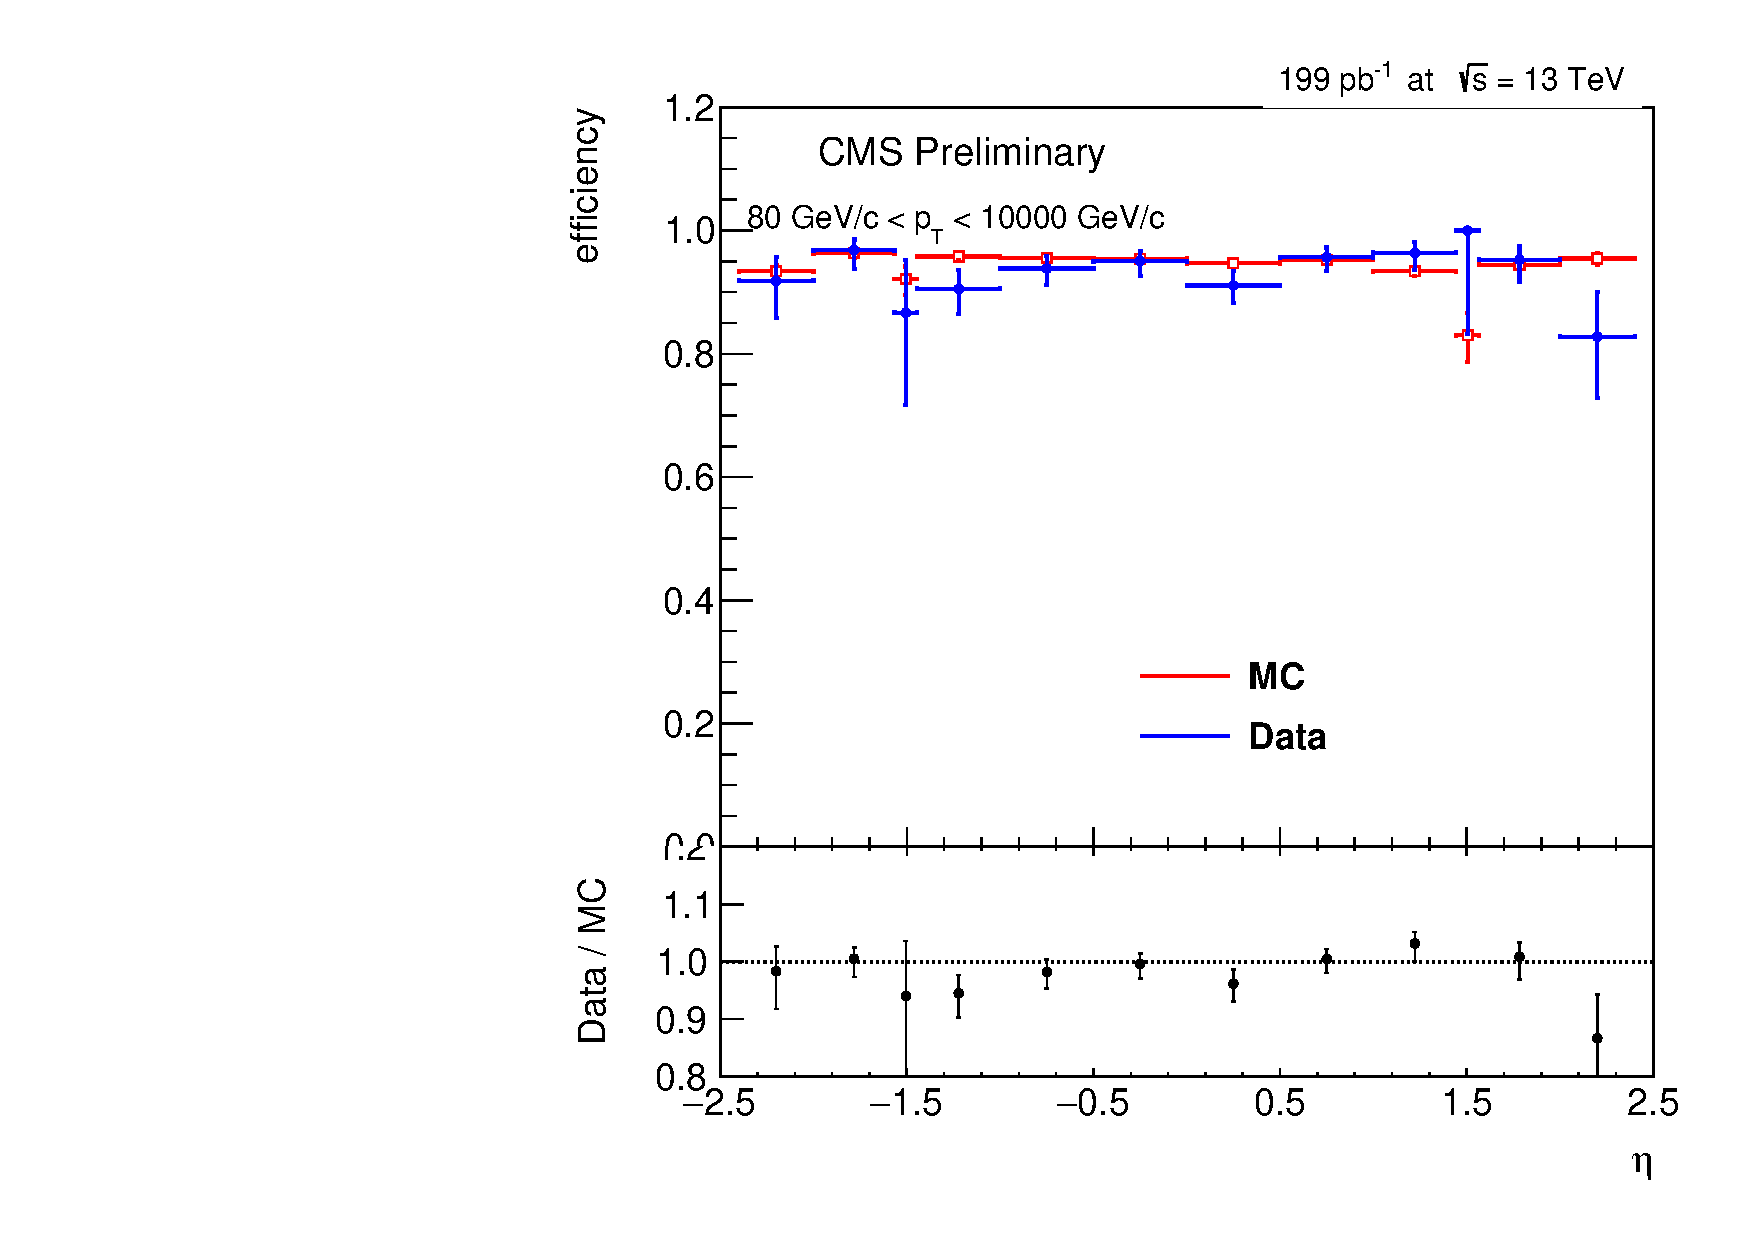
\includegraphics[width=0.45\linewidth]{plots/efficiency/13_zeehlt_negative/PtBins_eta_pt11.pdf}
\caption{$\eta$ dependence of Single electron trigger efficiency scale factors, separated by $p_T$ bins, for negatively charged electrons in the 13 TeV samples.}
\label{fig:Eff:el:13:HLT:neg}
\end{figure}


%%%% Figures for MuSIT Efficiency  %%%%%
\begin{figure}
\centering
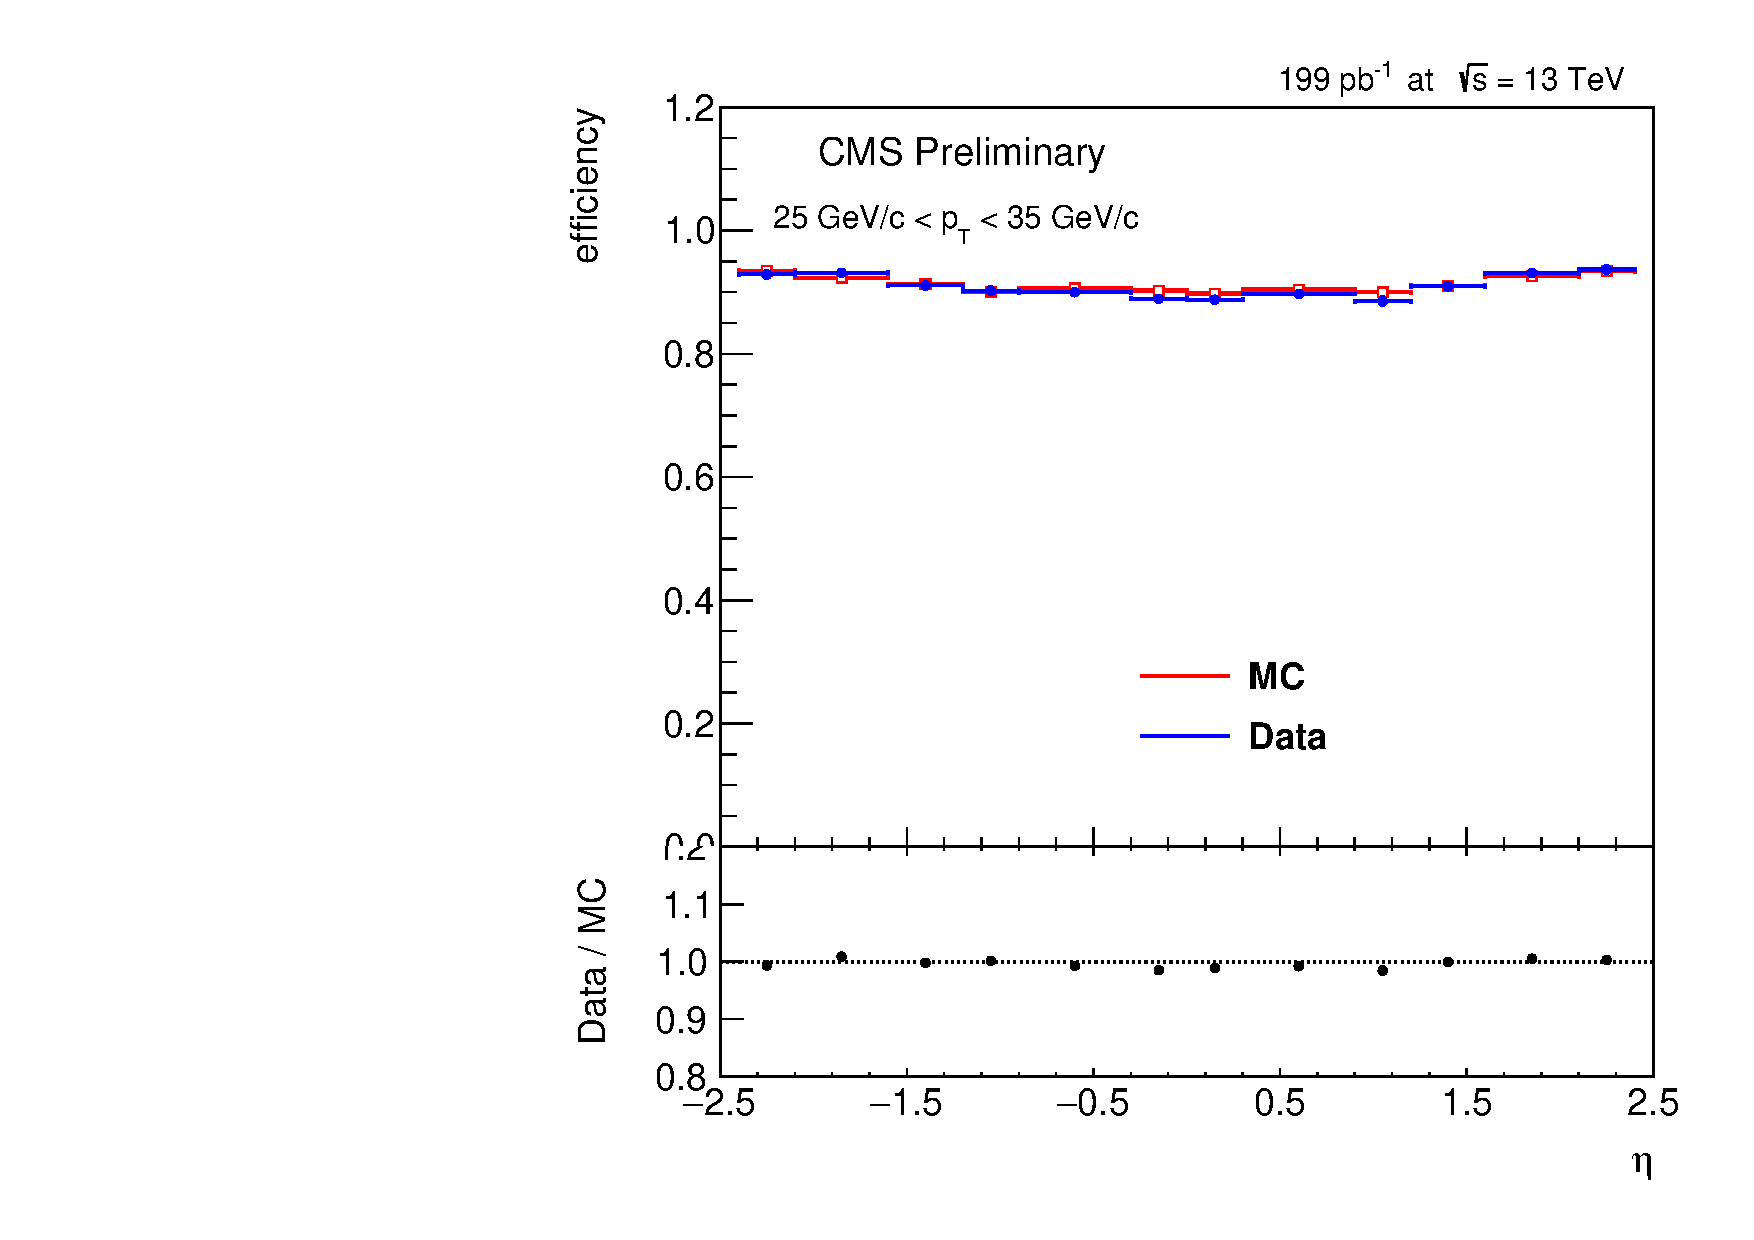
\includegraphics[width=0.32\linewidth]{plots/efficiency/13_zmmsit_combined/PtBins_eta_pt0.pdf}
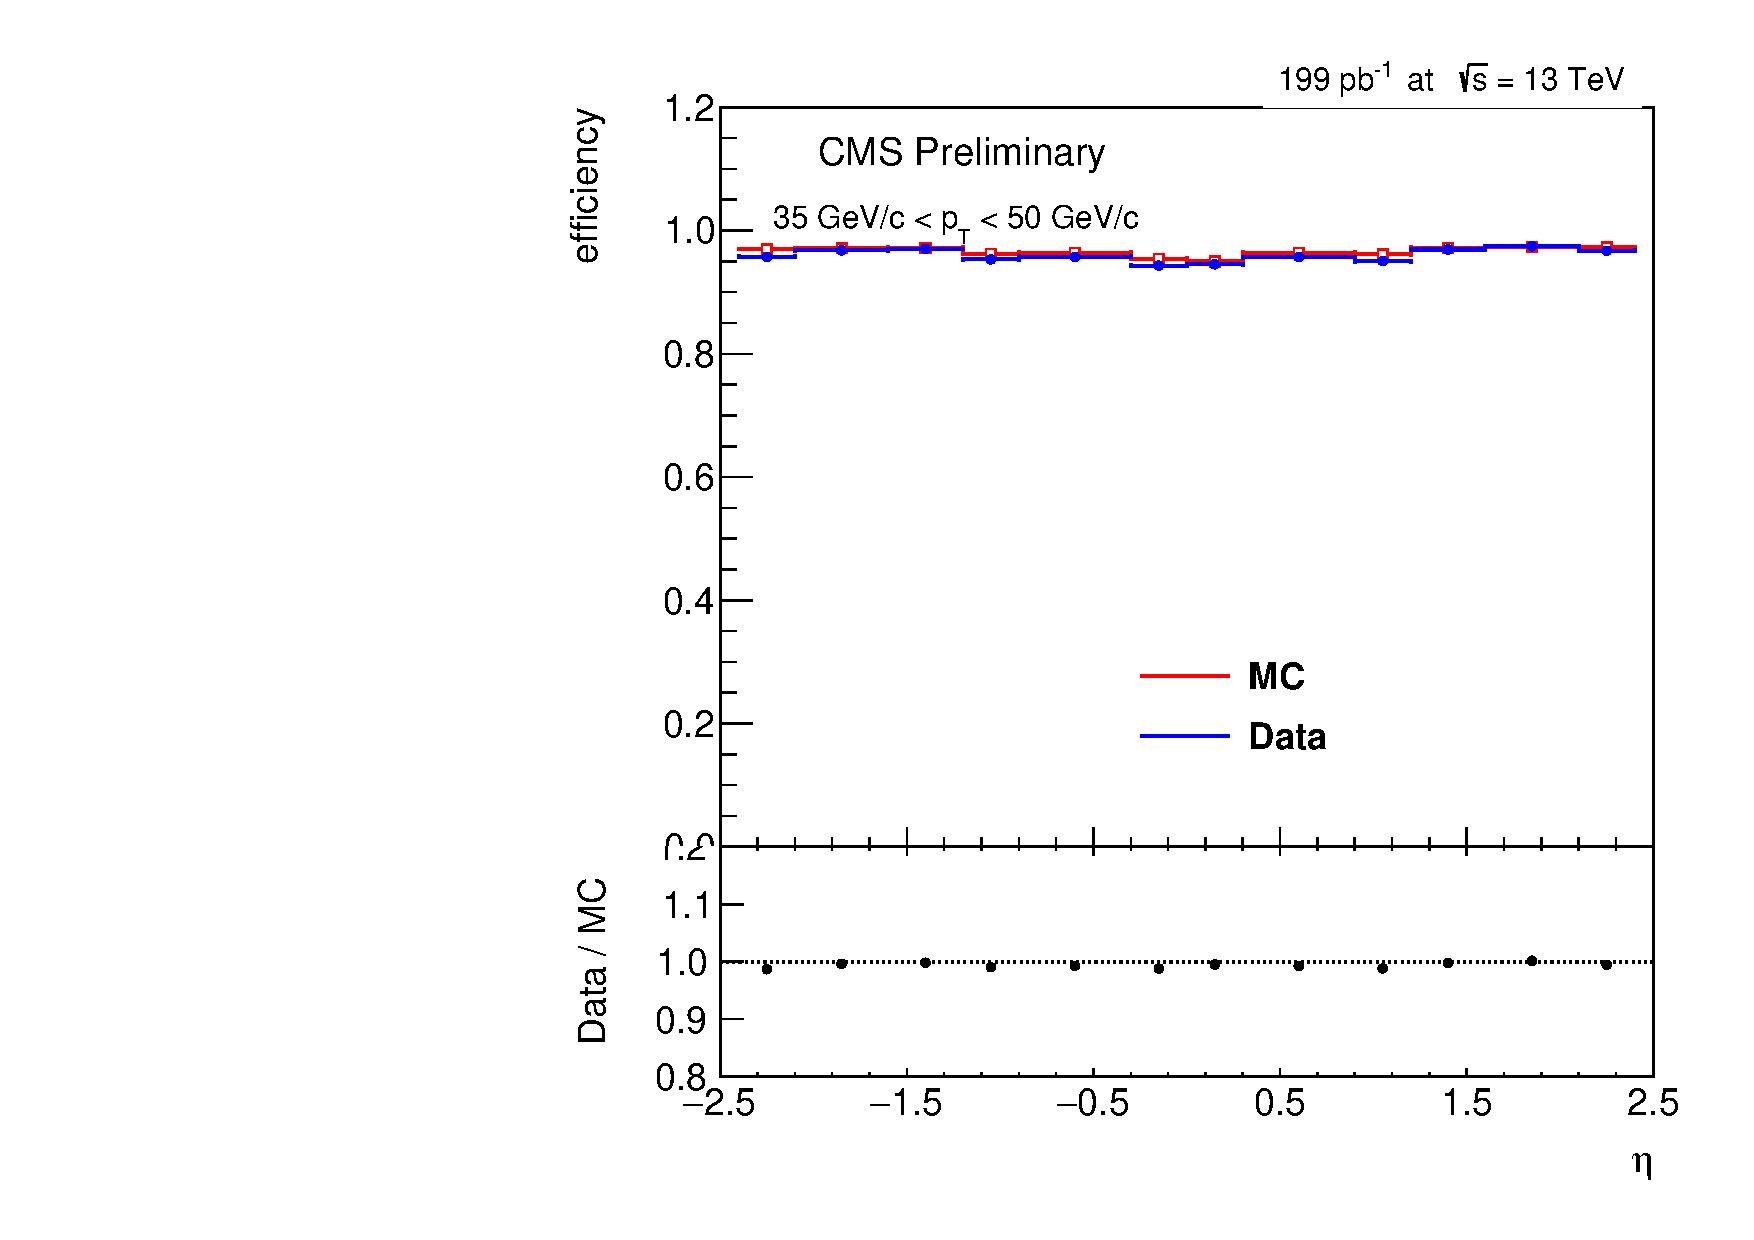
\includegraphics[width=0.32\linewidth]{plots/efficiency/13_zmmsit_combined/PtBins_eta_pt1.pdf}
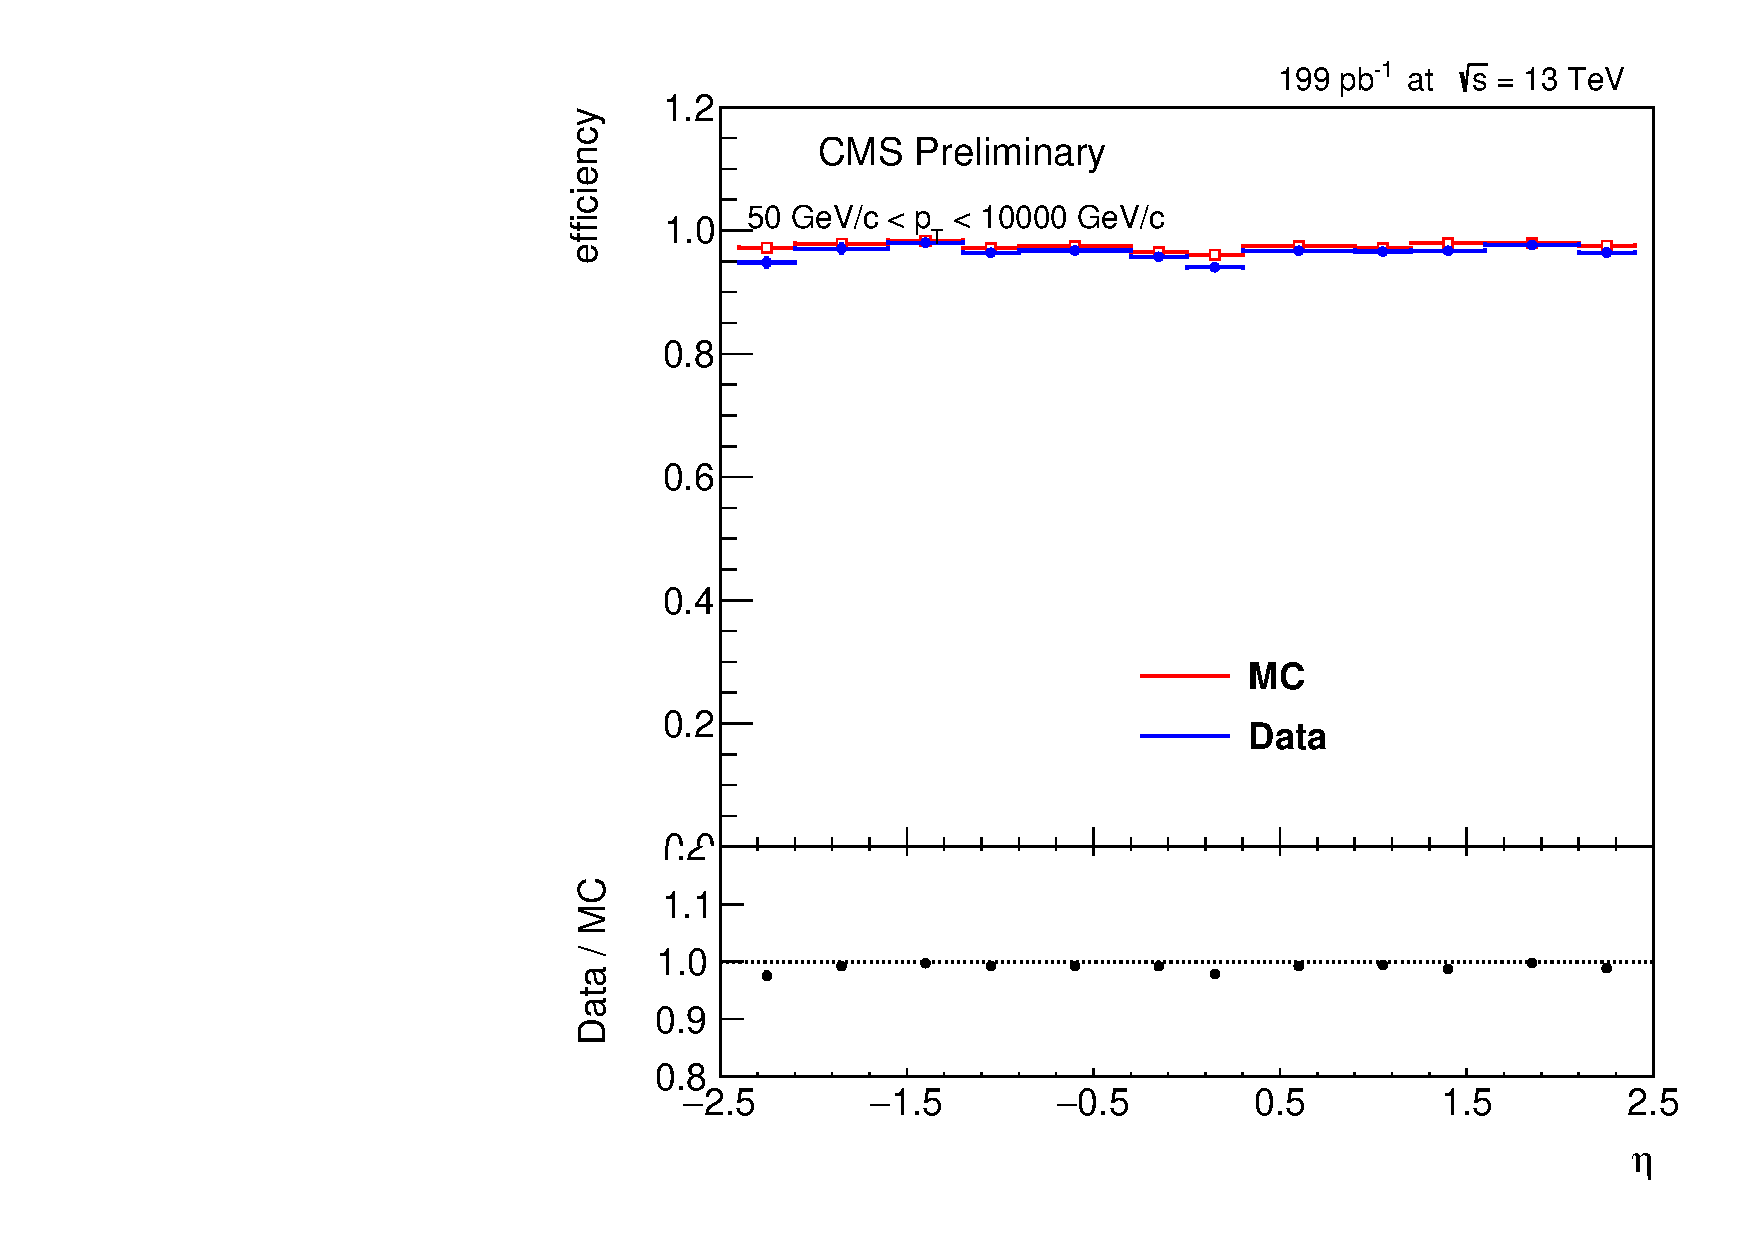
\includegraphics[width=0.32\linewidth]{plots/efficiency/13_zmmsit_combined/PtBins_eta_pt2.pdf}
\caption{$\eta$ dependence of Muon selection efficiency scale factors, separated by $p_T$ bins, for combined charged muons in the 13 TeV samples.}
\label{fig:Eff:mu:13:SIT:com}
\end{figure}

%%%% Figures for MuSta Efficiency  %%%%%
\begin{figure}
\centering
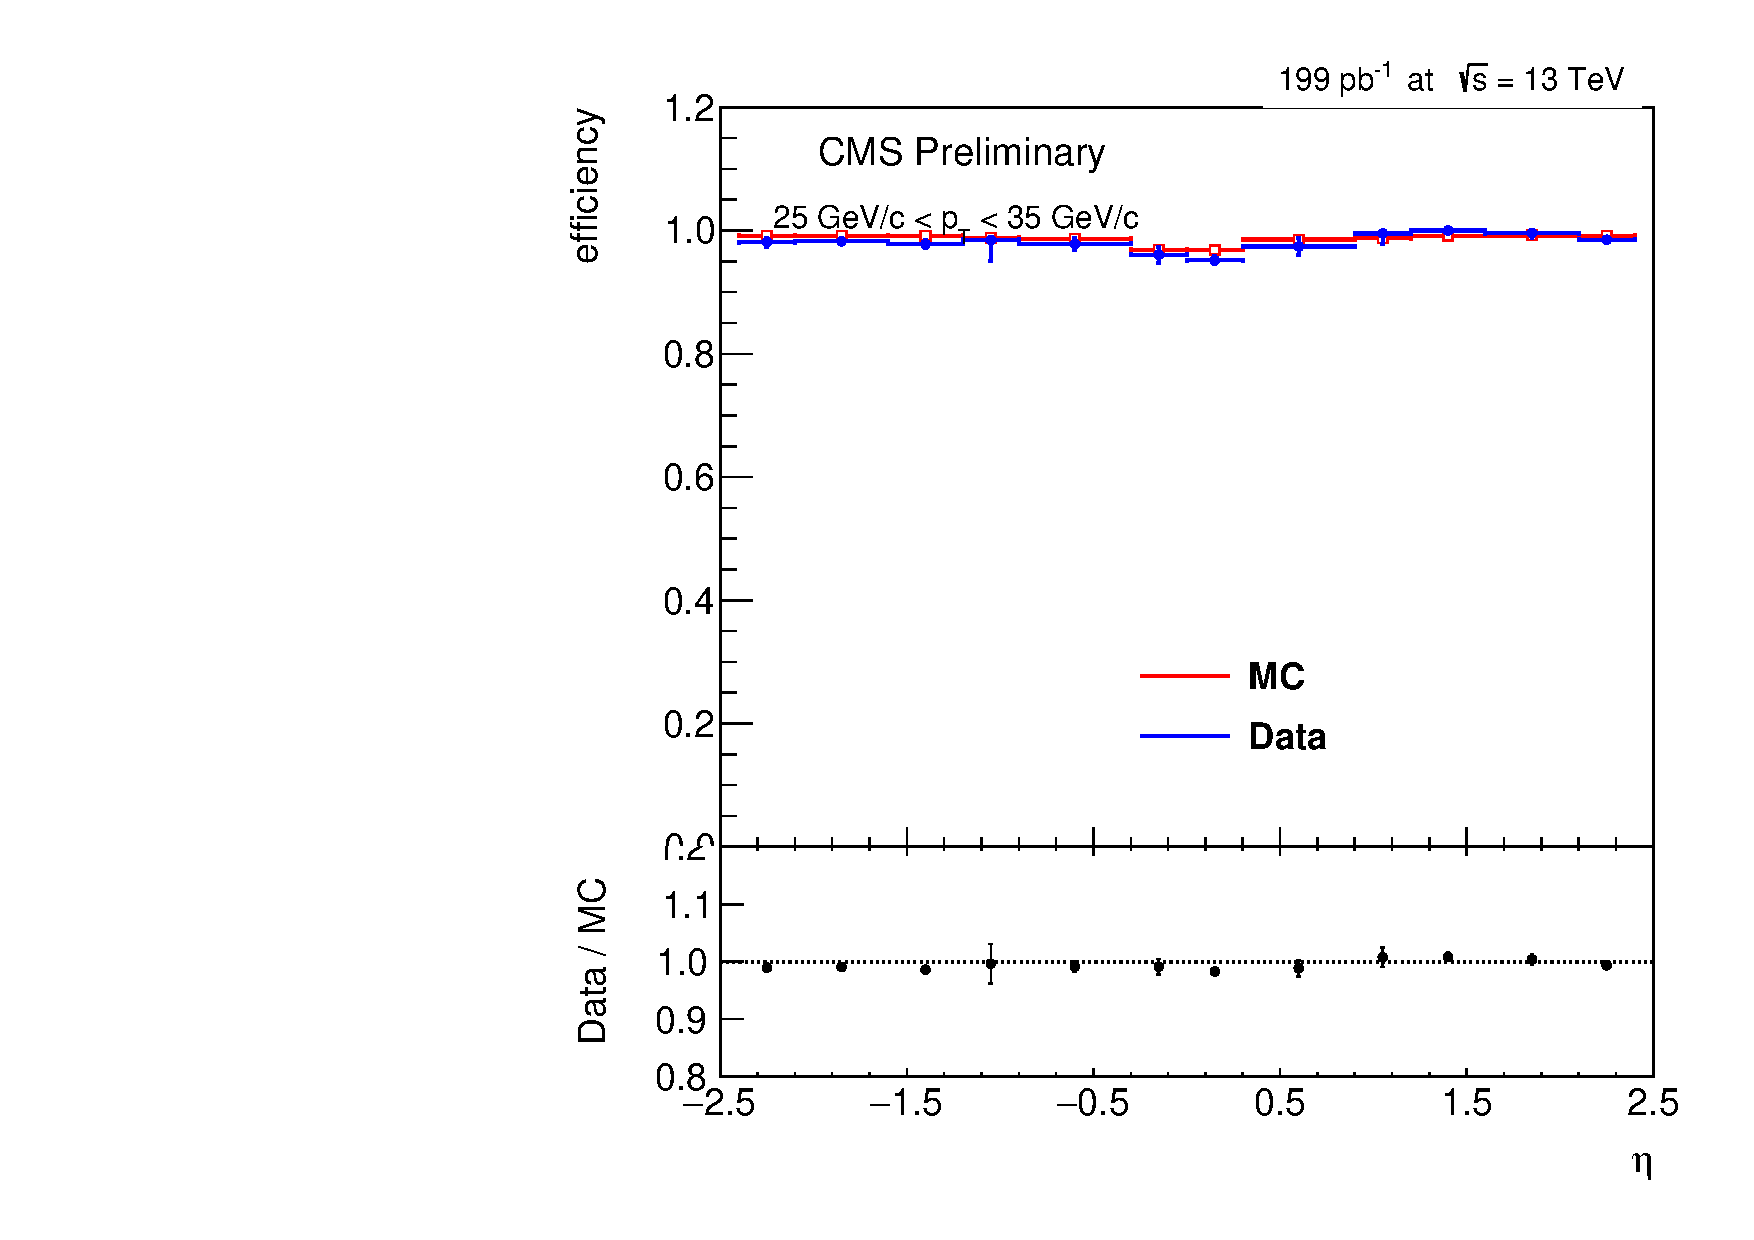
\includegraphics[width=0.32\linewidth]{plots/efficiency/13_zmmsta_combined/PtBins_eta_pt0.pdf}
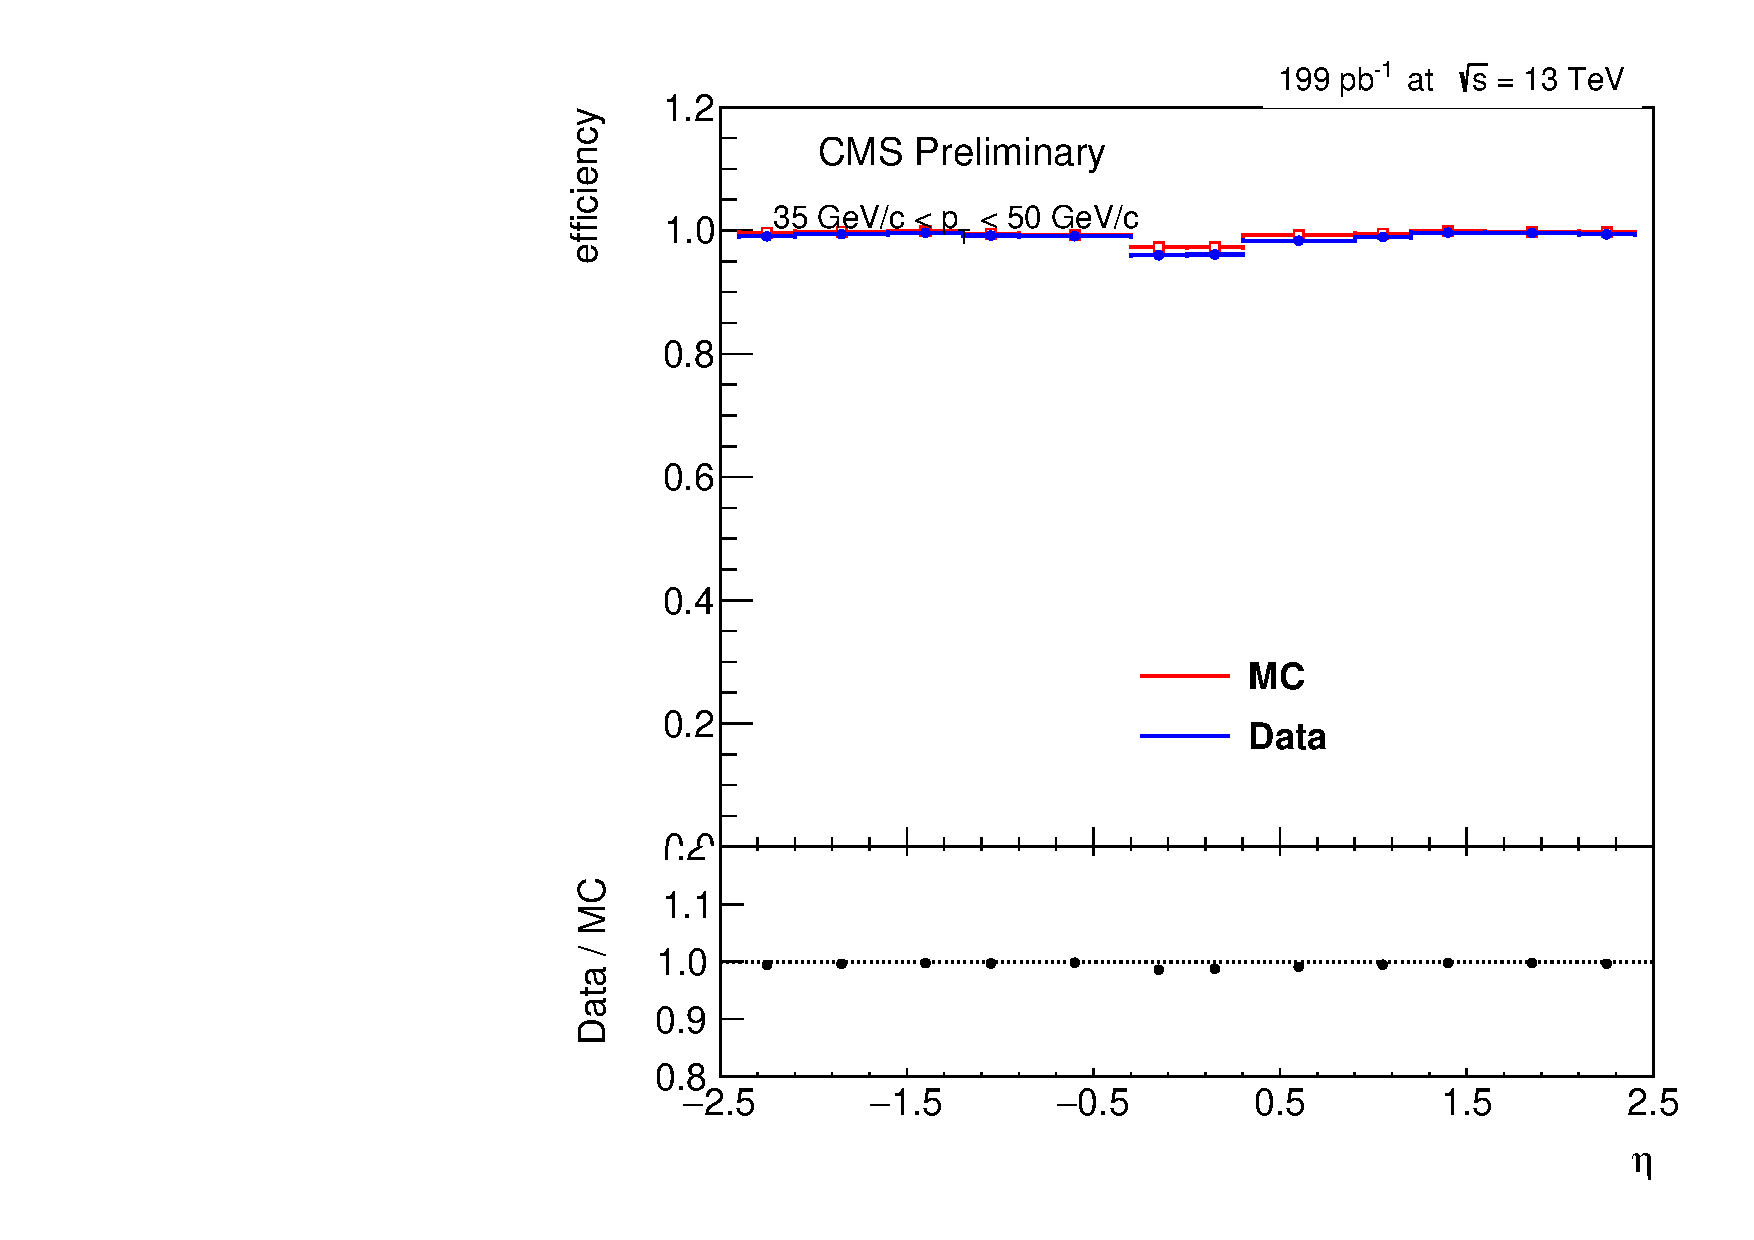
\includegraphics[width=0.32\linewidth]{plots/efficiency/13_zmmsta_combined/PtBins_eta_pt1.pdf}
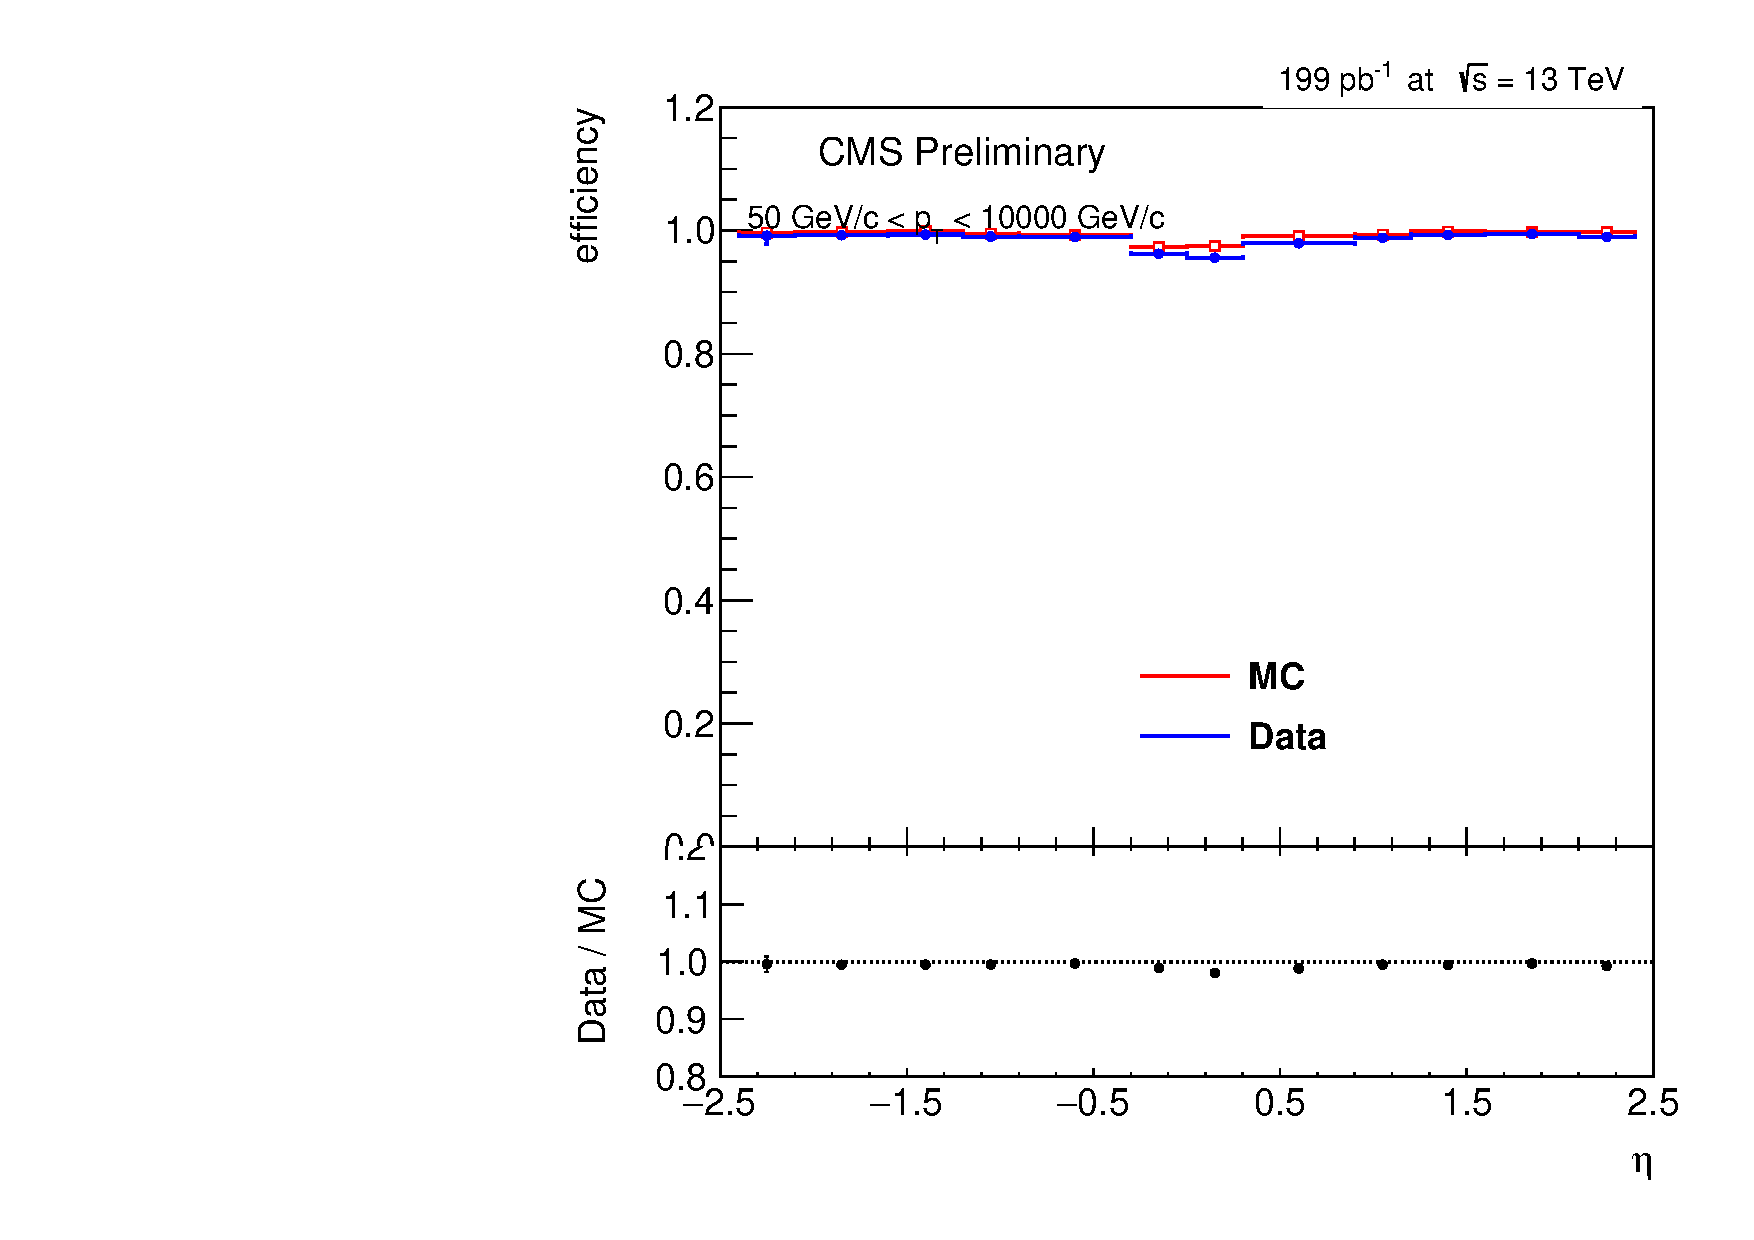
\includegraphics[width=0.32\linewidth]{plots/efficiency/13_zmmsta_combined/PtBins_eta_pt2.pdf}
\caption{$\eta$ dependence of Standalone muon identification efficiency scale factors, separated by $p_T$ bins, for combined charged muons in the 13 TeV samples.}
\label{fig:Eff:mu:13:Sta:com}
\end{figure}

%%%% Figures for MuHLT Efficiency  %%%%%
\begin{figure}
\centering
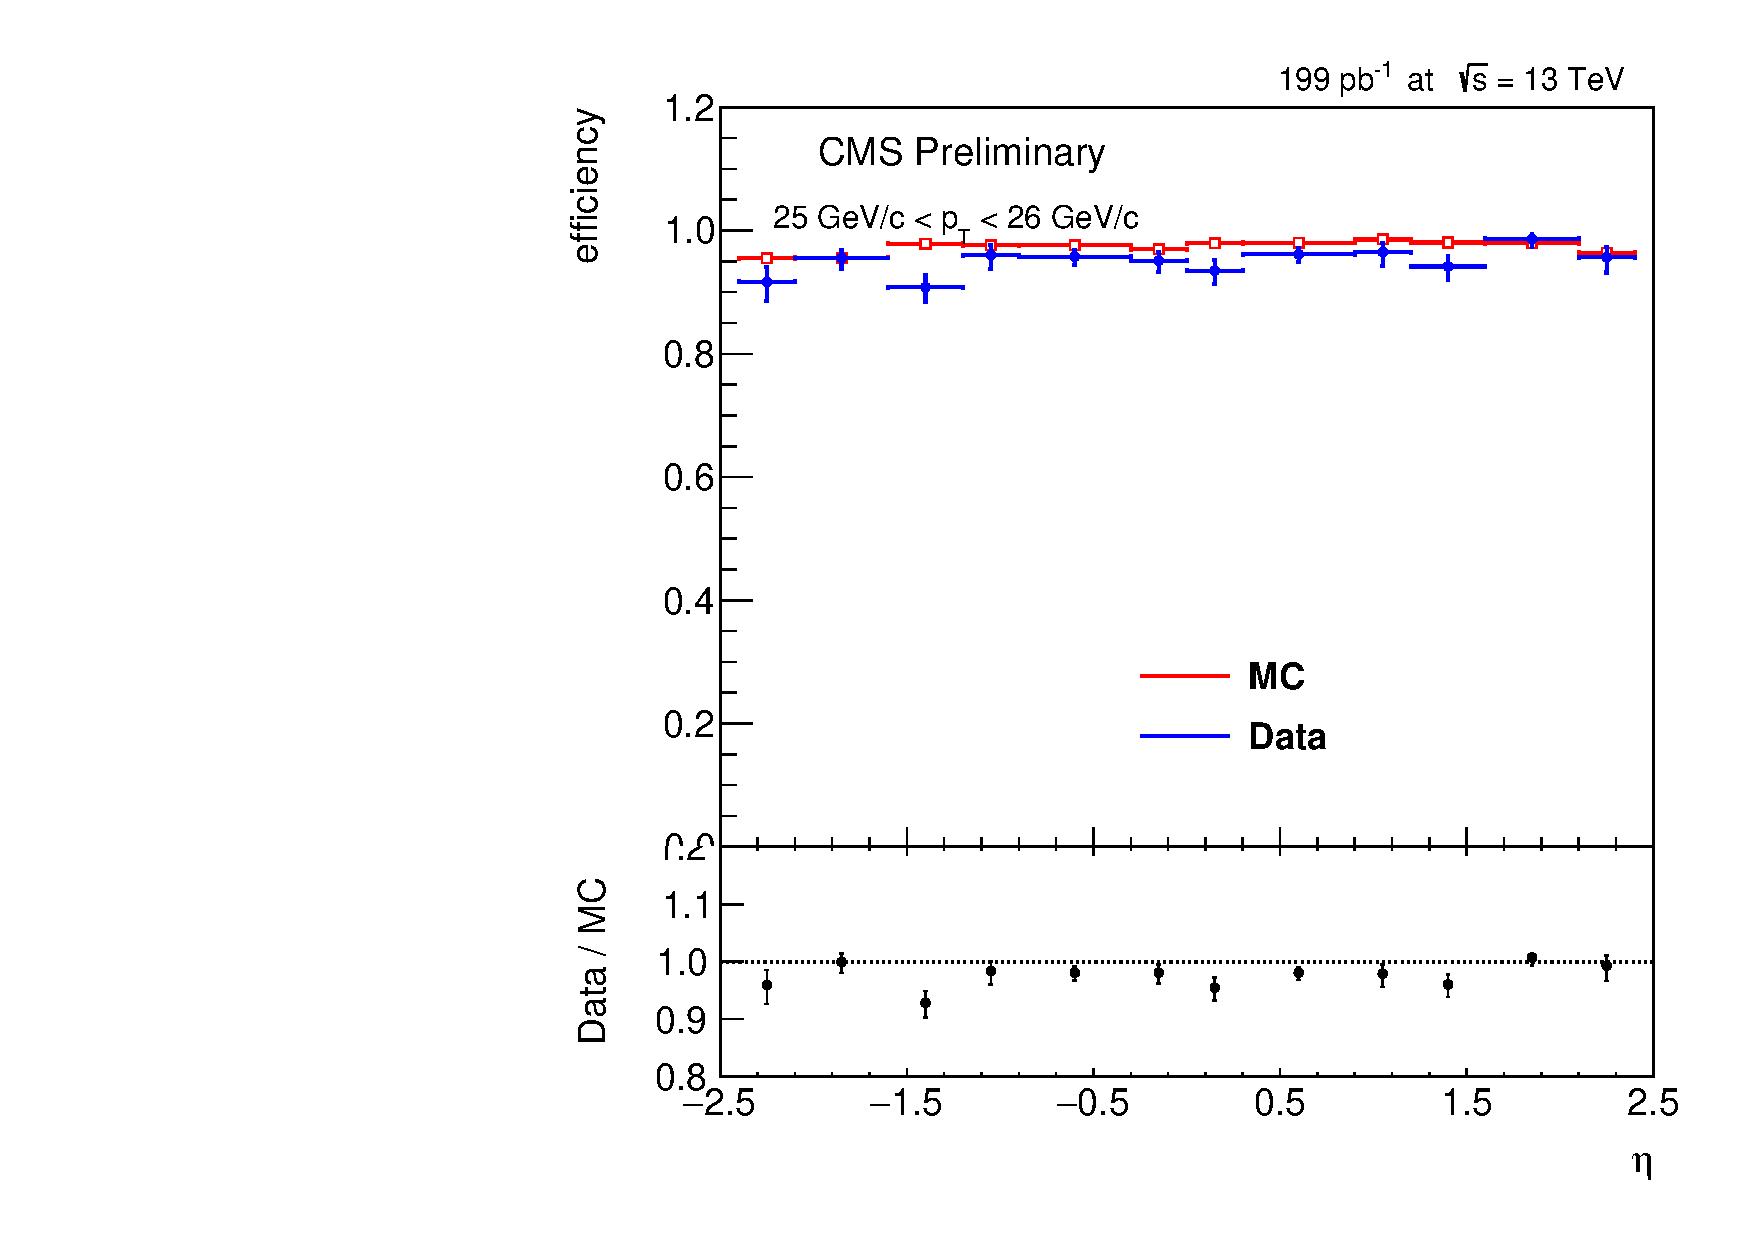
\includegraphics[width=0.32\linewidth]{plots/efficiency/13_zmmhlt_positive/PtBins_eta_pt0.pdf}
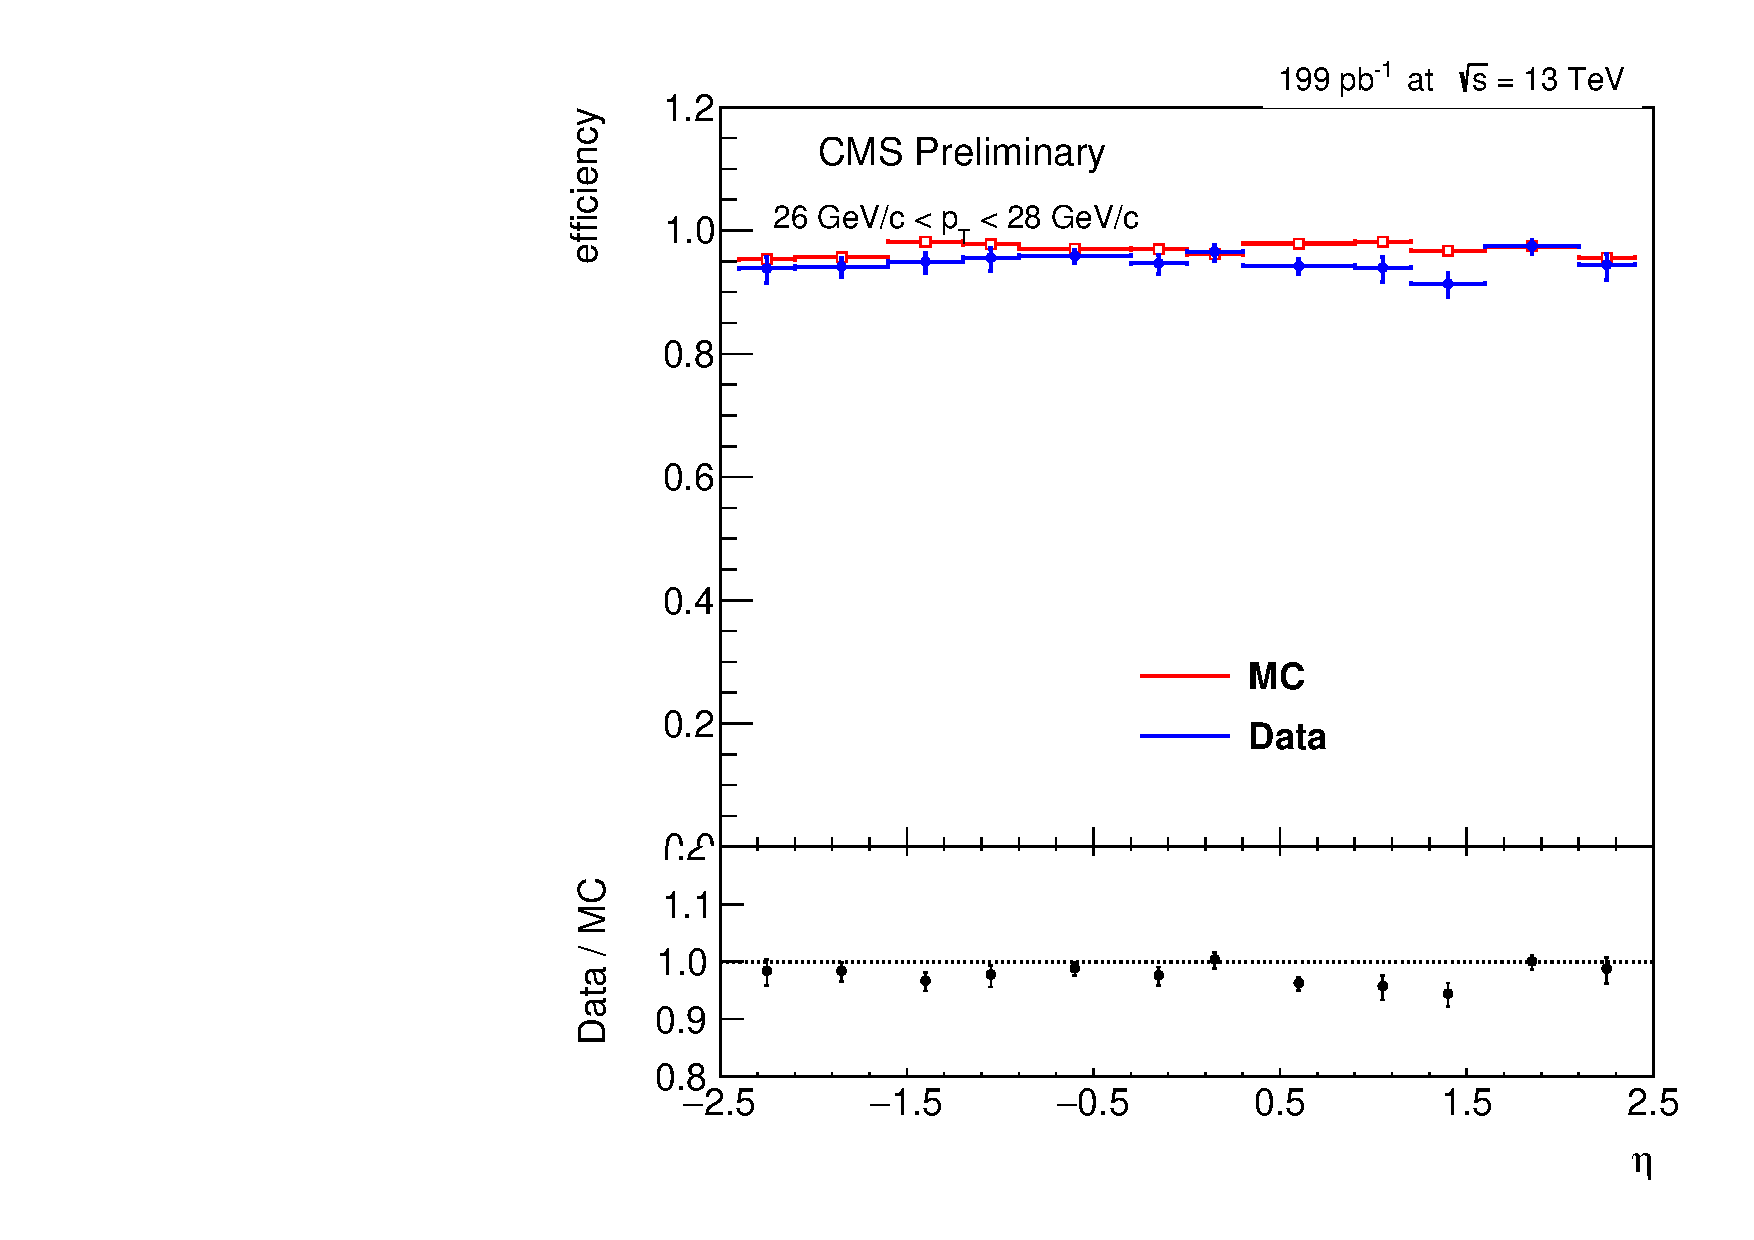
\includegraphics[width=0.32\linewidth]{plots/efficiency/13_zmmhlt_positive/PtBins_eta_pt1.pdf}
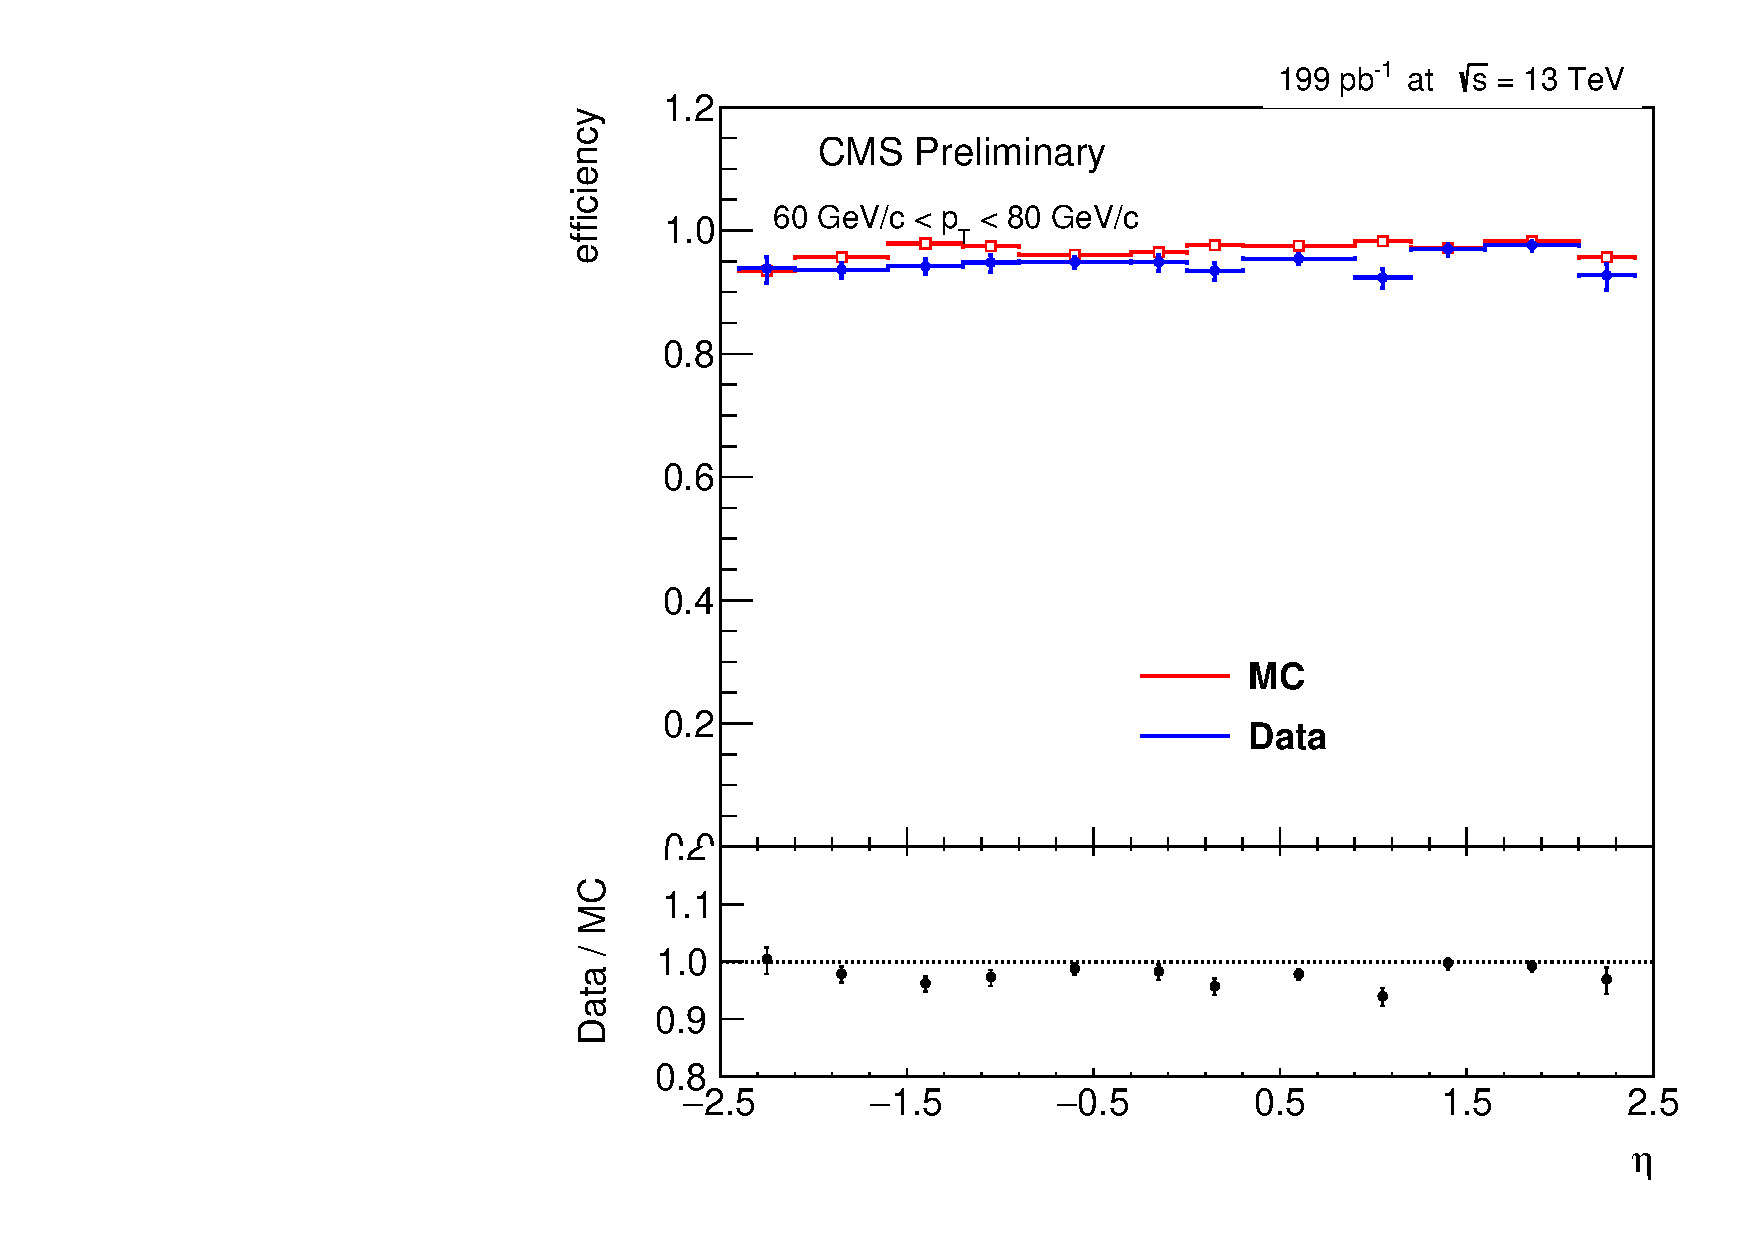
\includegraphics[width=0.32\linewidth]{plots/efficiency/13_zmmhlt_positive/PtBins_eta_pt10.pdf}
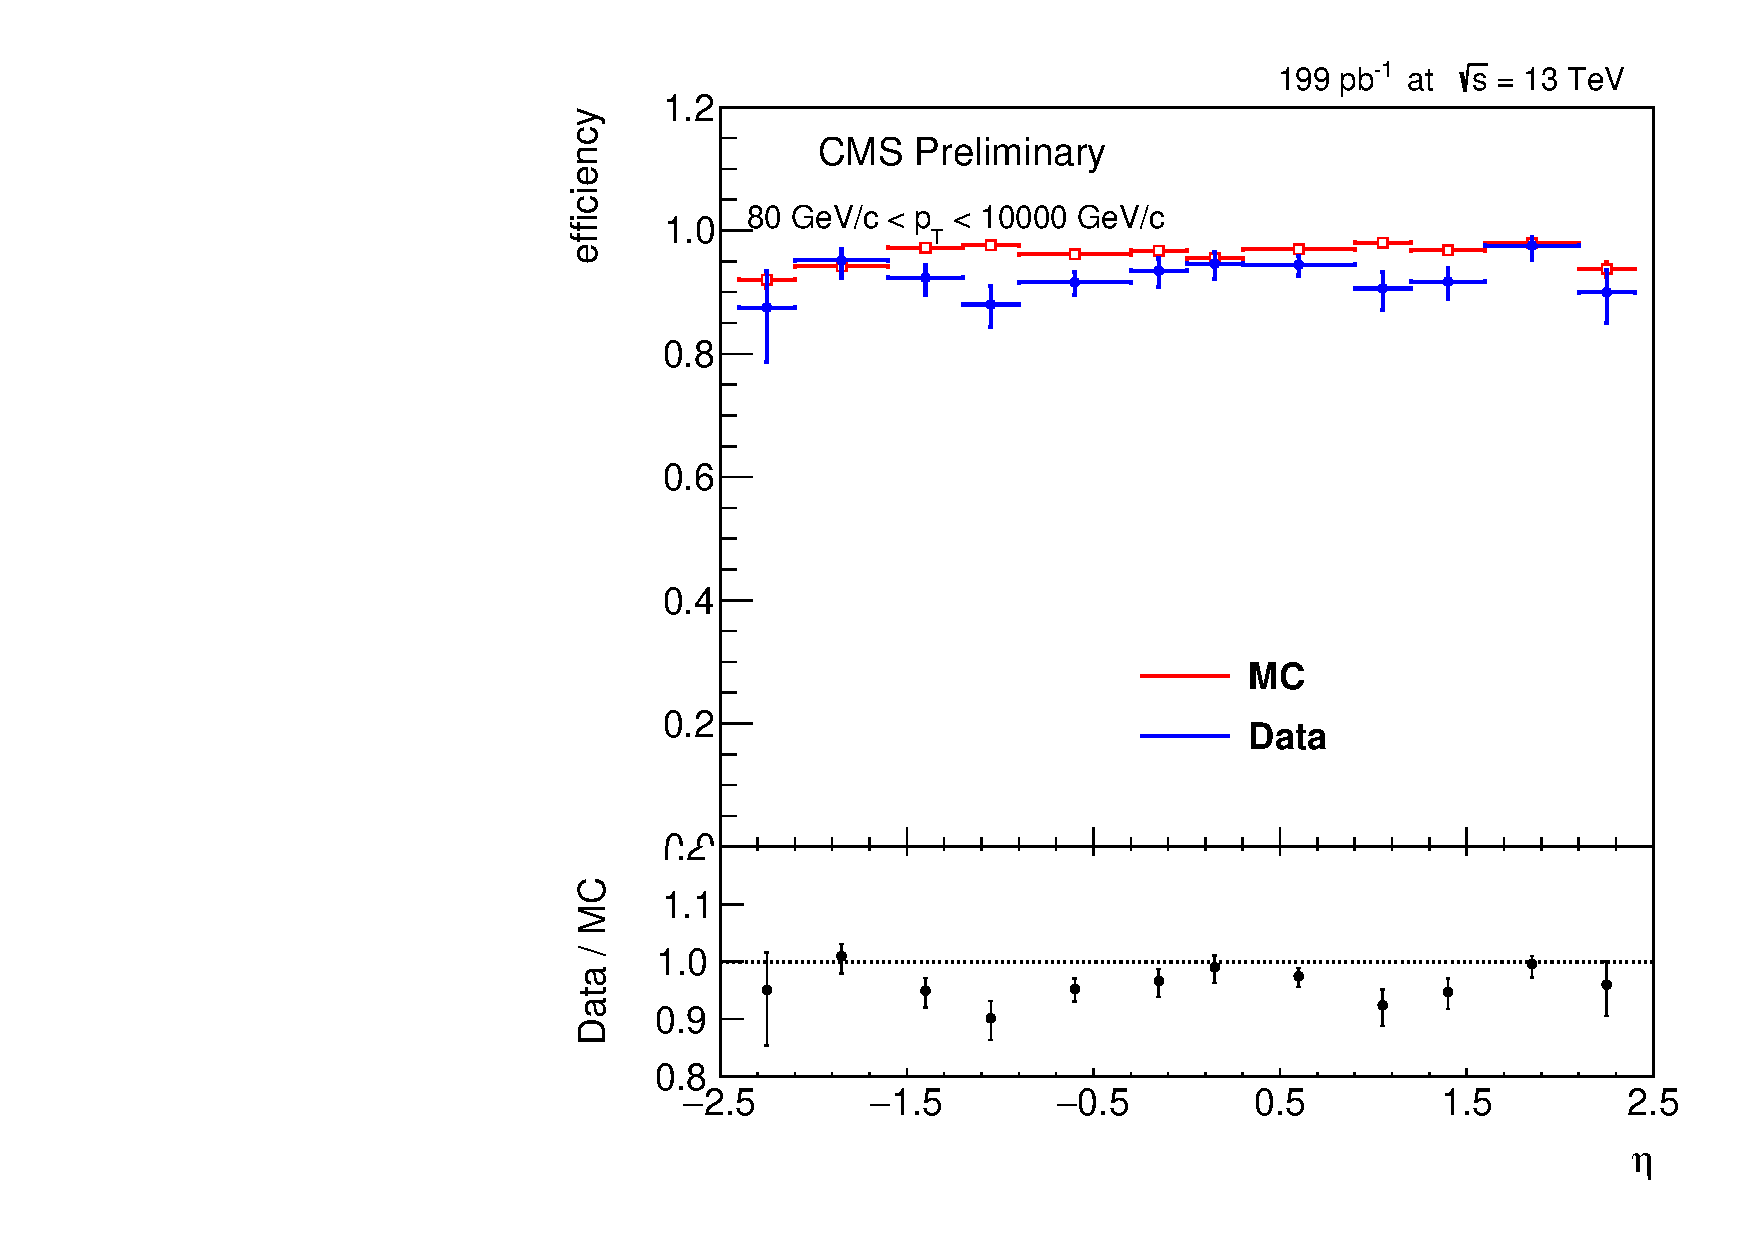
\includegraphics[width=0.32\linewidth]{plots/efficiency/13_zmmhlt_positive/PtBins_eta_pt11.pdf}
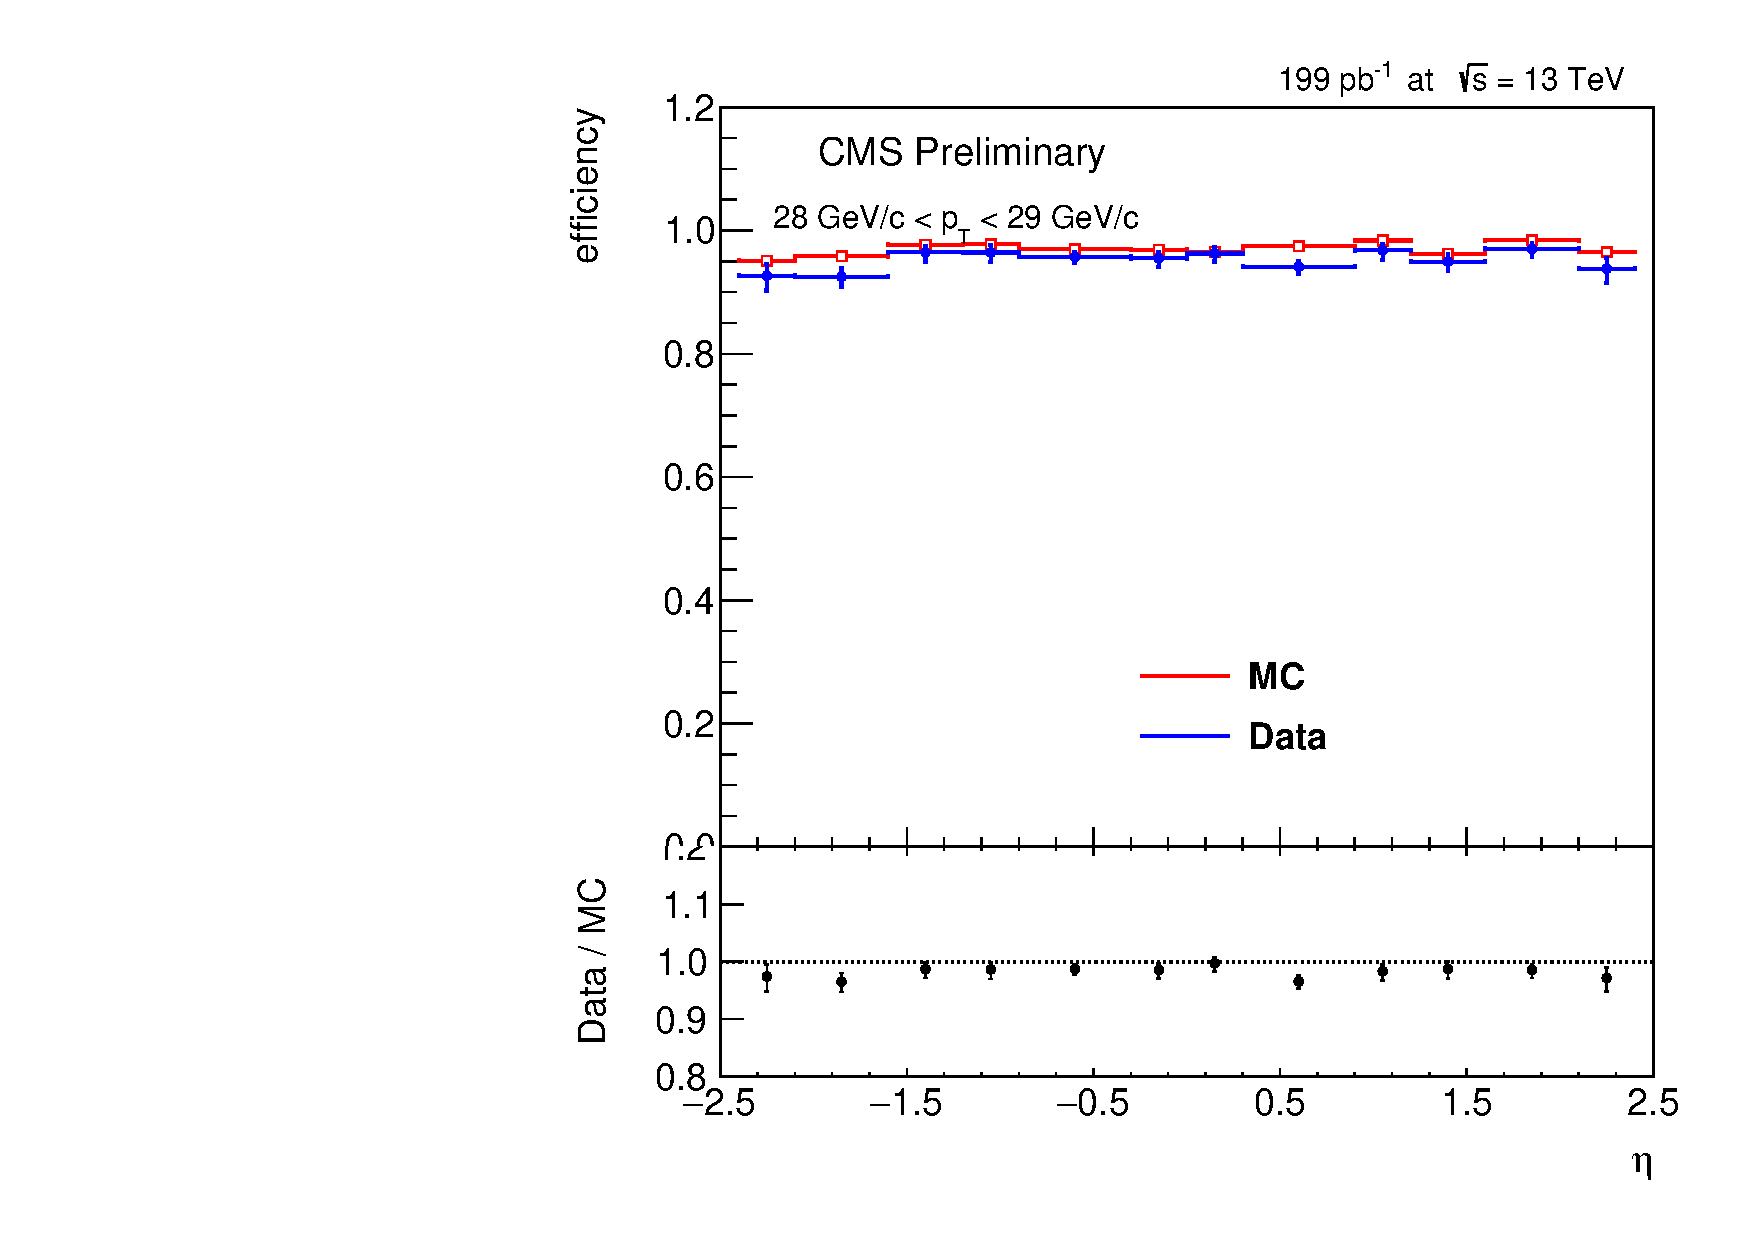
\includegraphics[width=0.32\linewidth]{plots/efficiency/13_zmmhlt_positive/PtBins_eta_pt2.pdf}
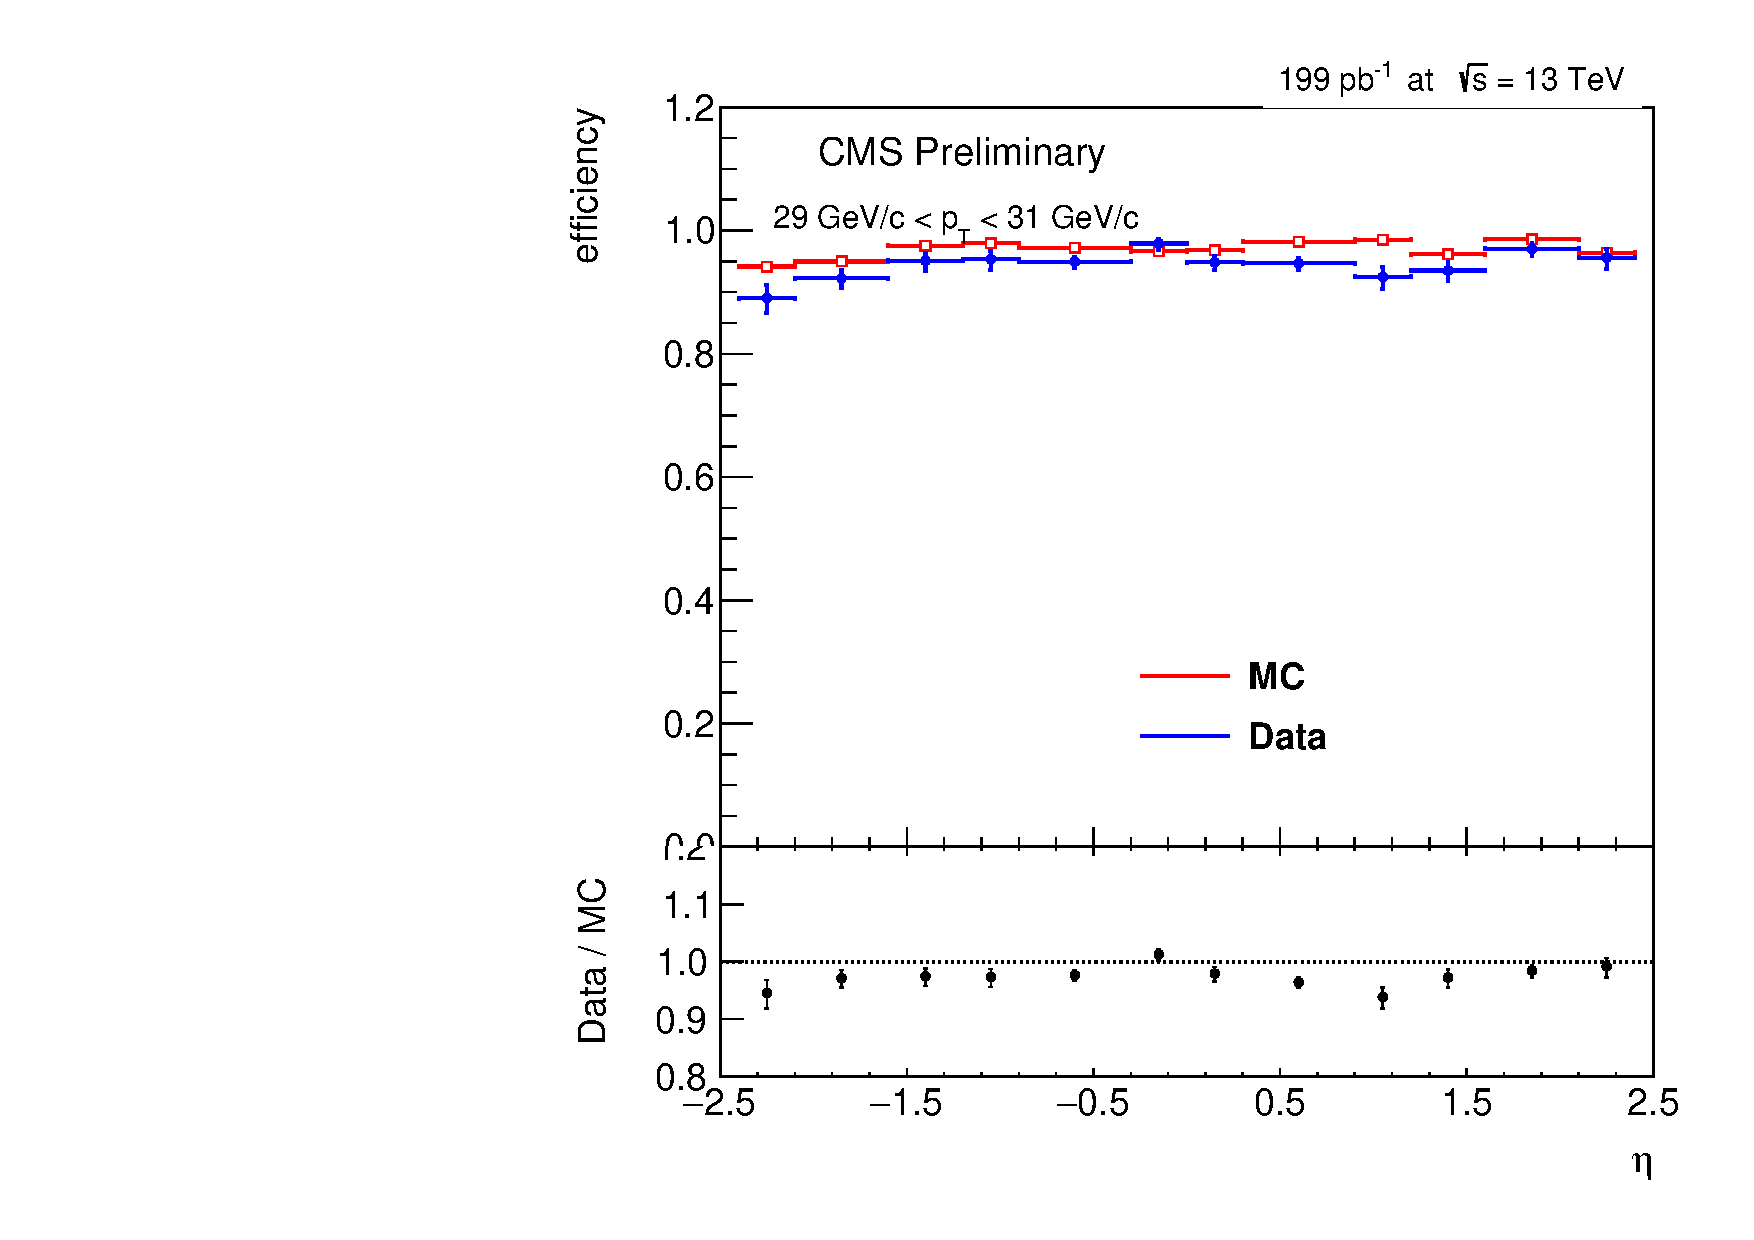
\includegraphics[width=0.32\linewidth]{plots/efficiency/13_zmmhlt_positive/PtBins_eta_pt3.pdf}
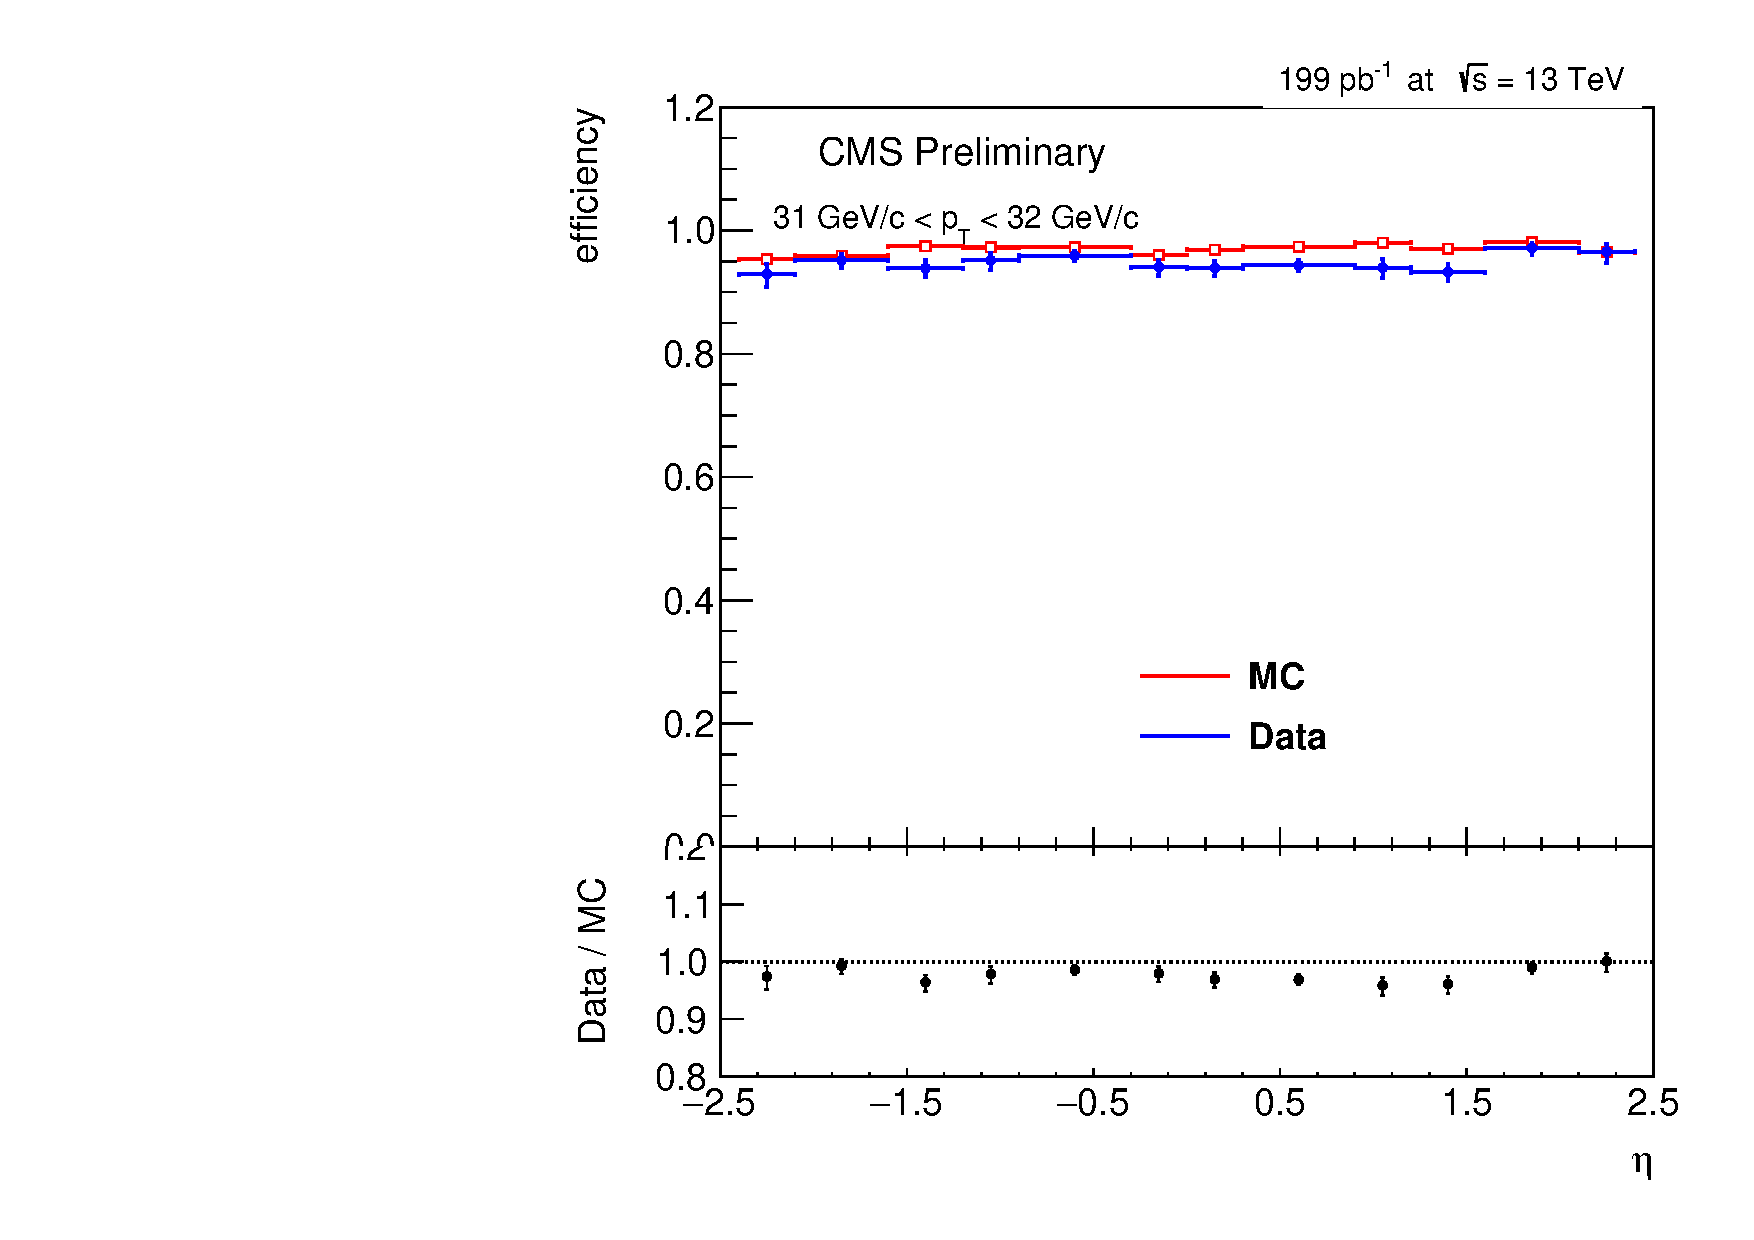
\includegraphics[width=0.32\linewidth]{plots/efficiency/13_zmmhlt_positive/PtBins_eta_pt4.pdf}
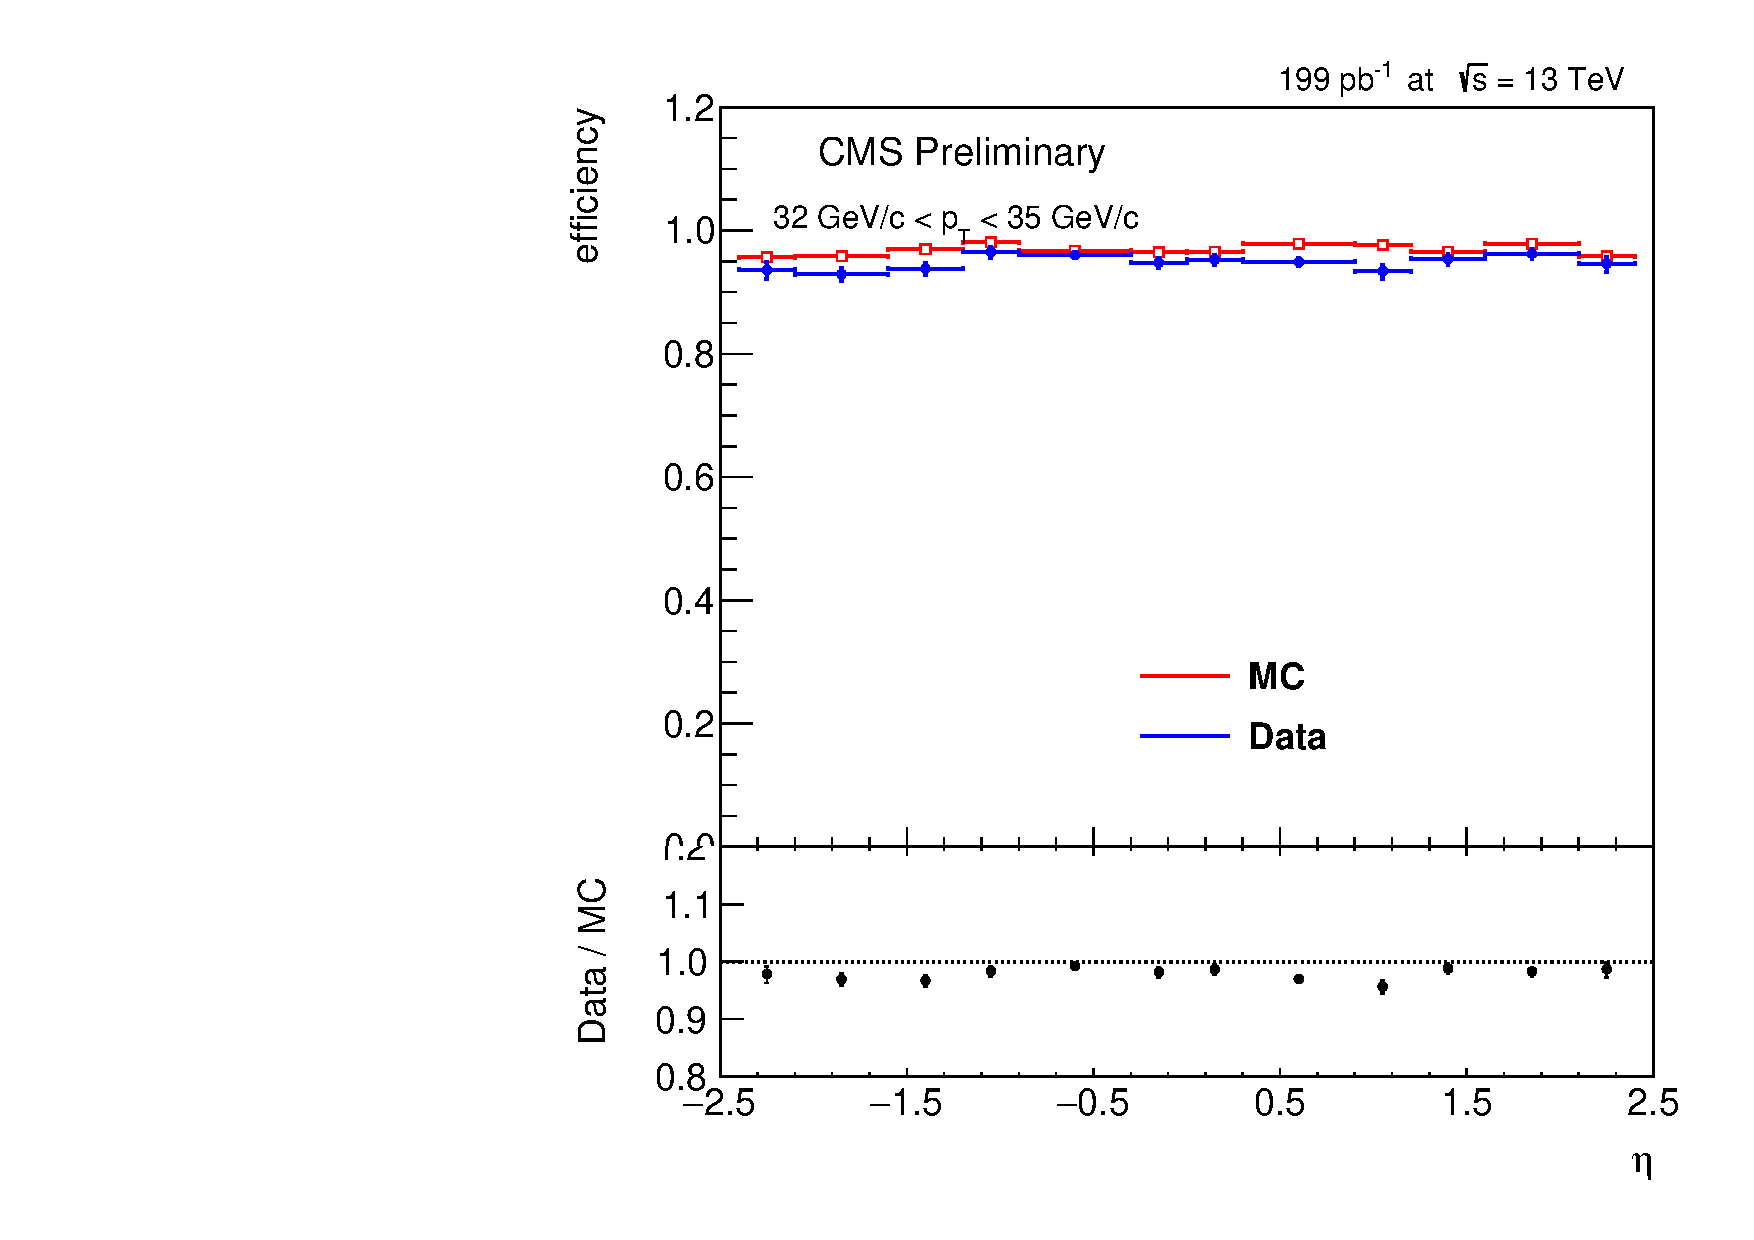
\includegraphics[width=0.32\linewidth]{plots/efficiency/13_zmmhlt_positive/PtBins_eta_pt5.pdf}
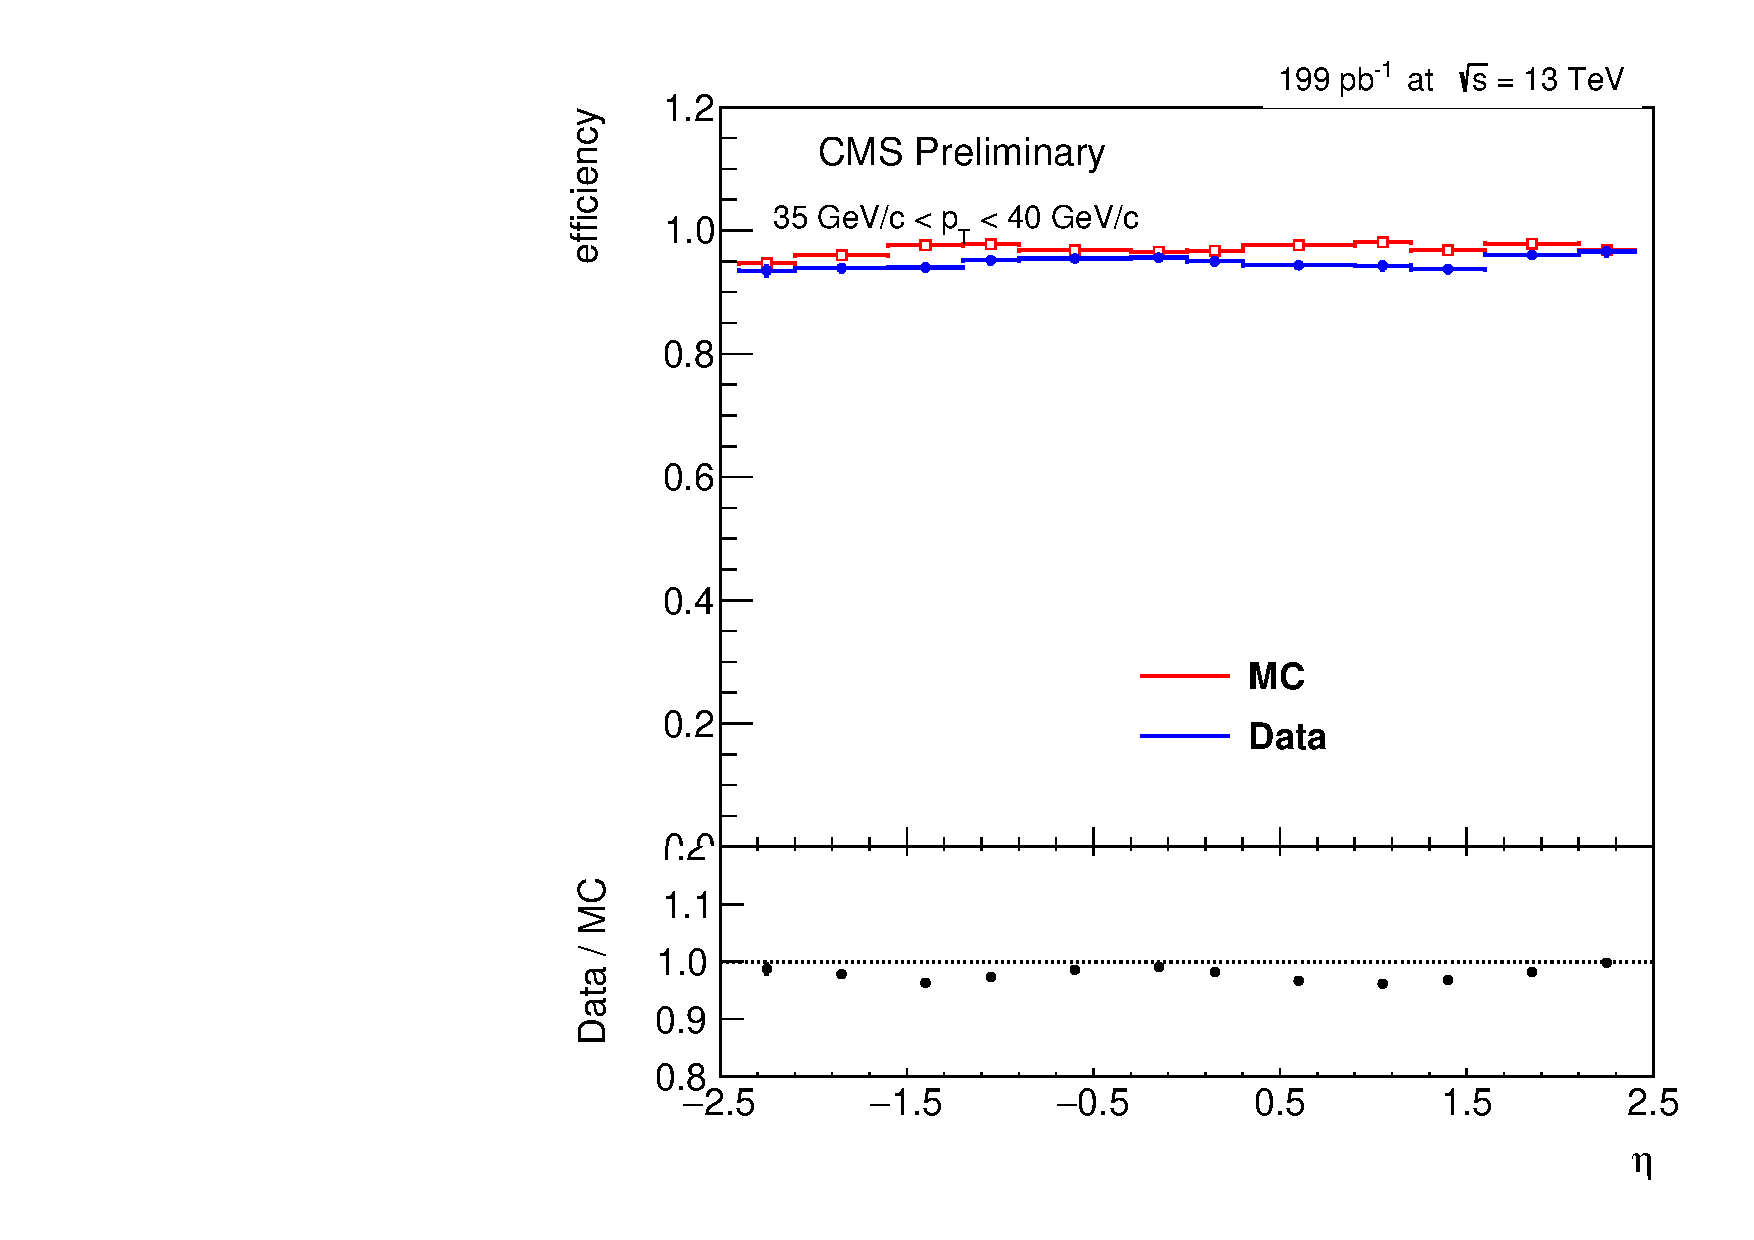
\includegraphics[width=0.32\linewidth]{plots/efficiency/13_zmmhlt_positive/PtBins_eta_pt6.pdf}
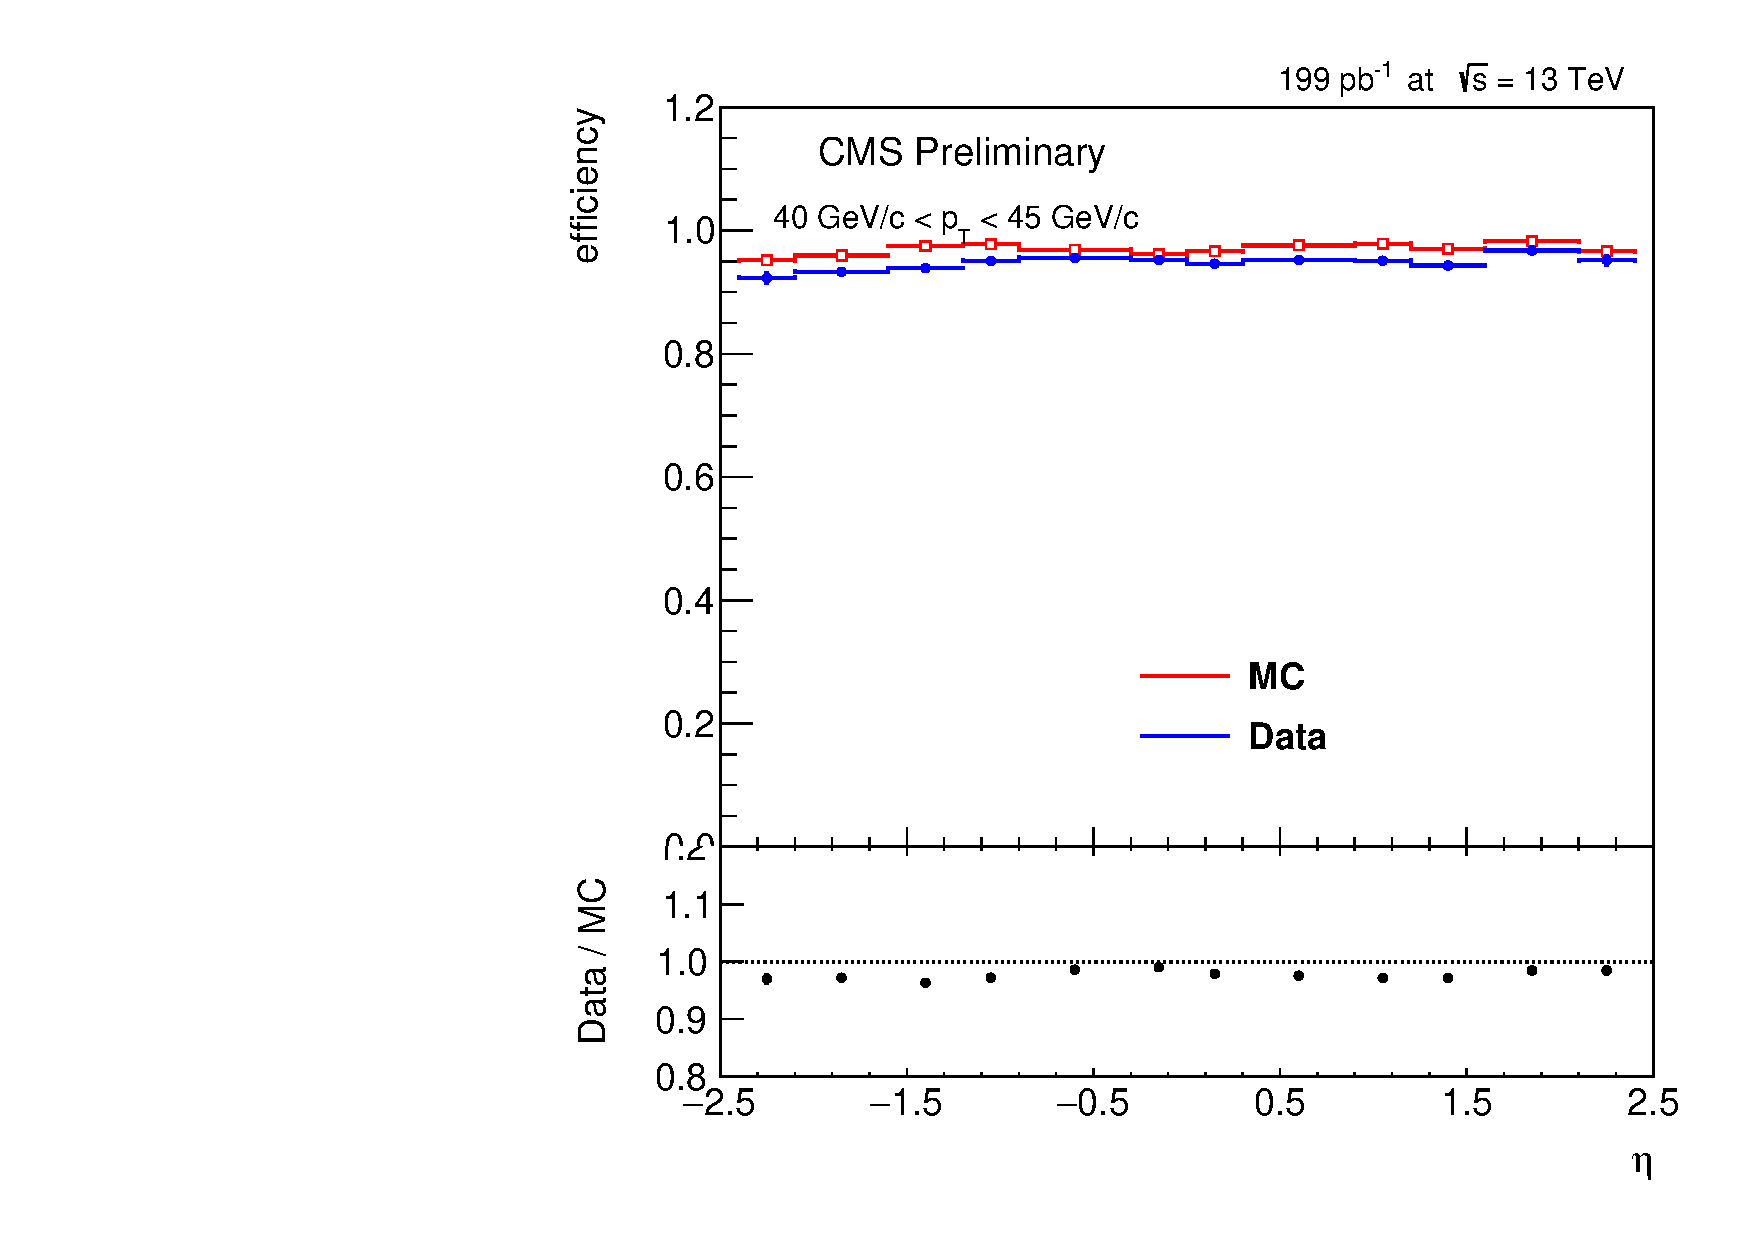
\includegraphics[width=0.32\linewidth]{plots/efficiency/13_zmmhlt_positive/PtBins_eta_pt7.pdf}
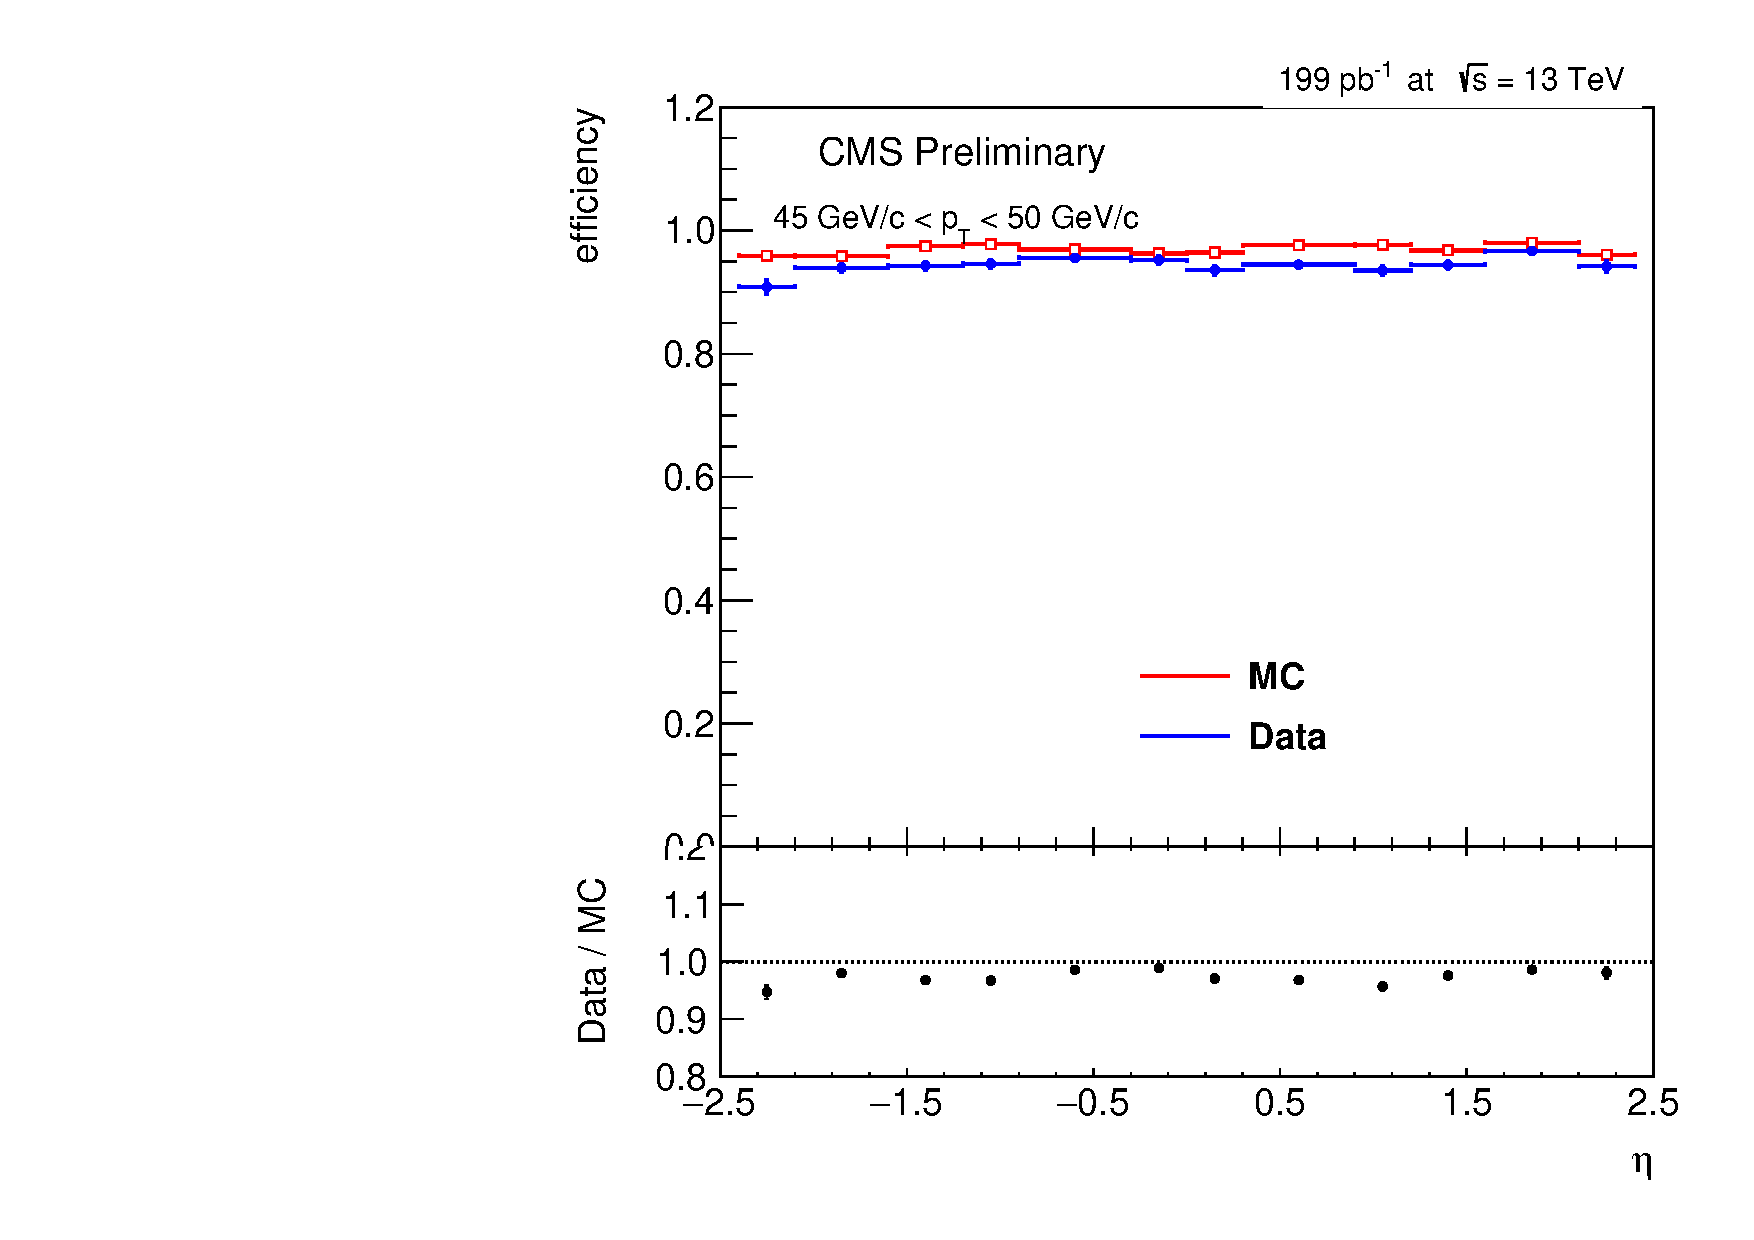
\includegraphics[width=0.32\linewidth]{plots/efficiency/13_zmmhlt_positive/PtBins_eta_pt8.pdf}
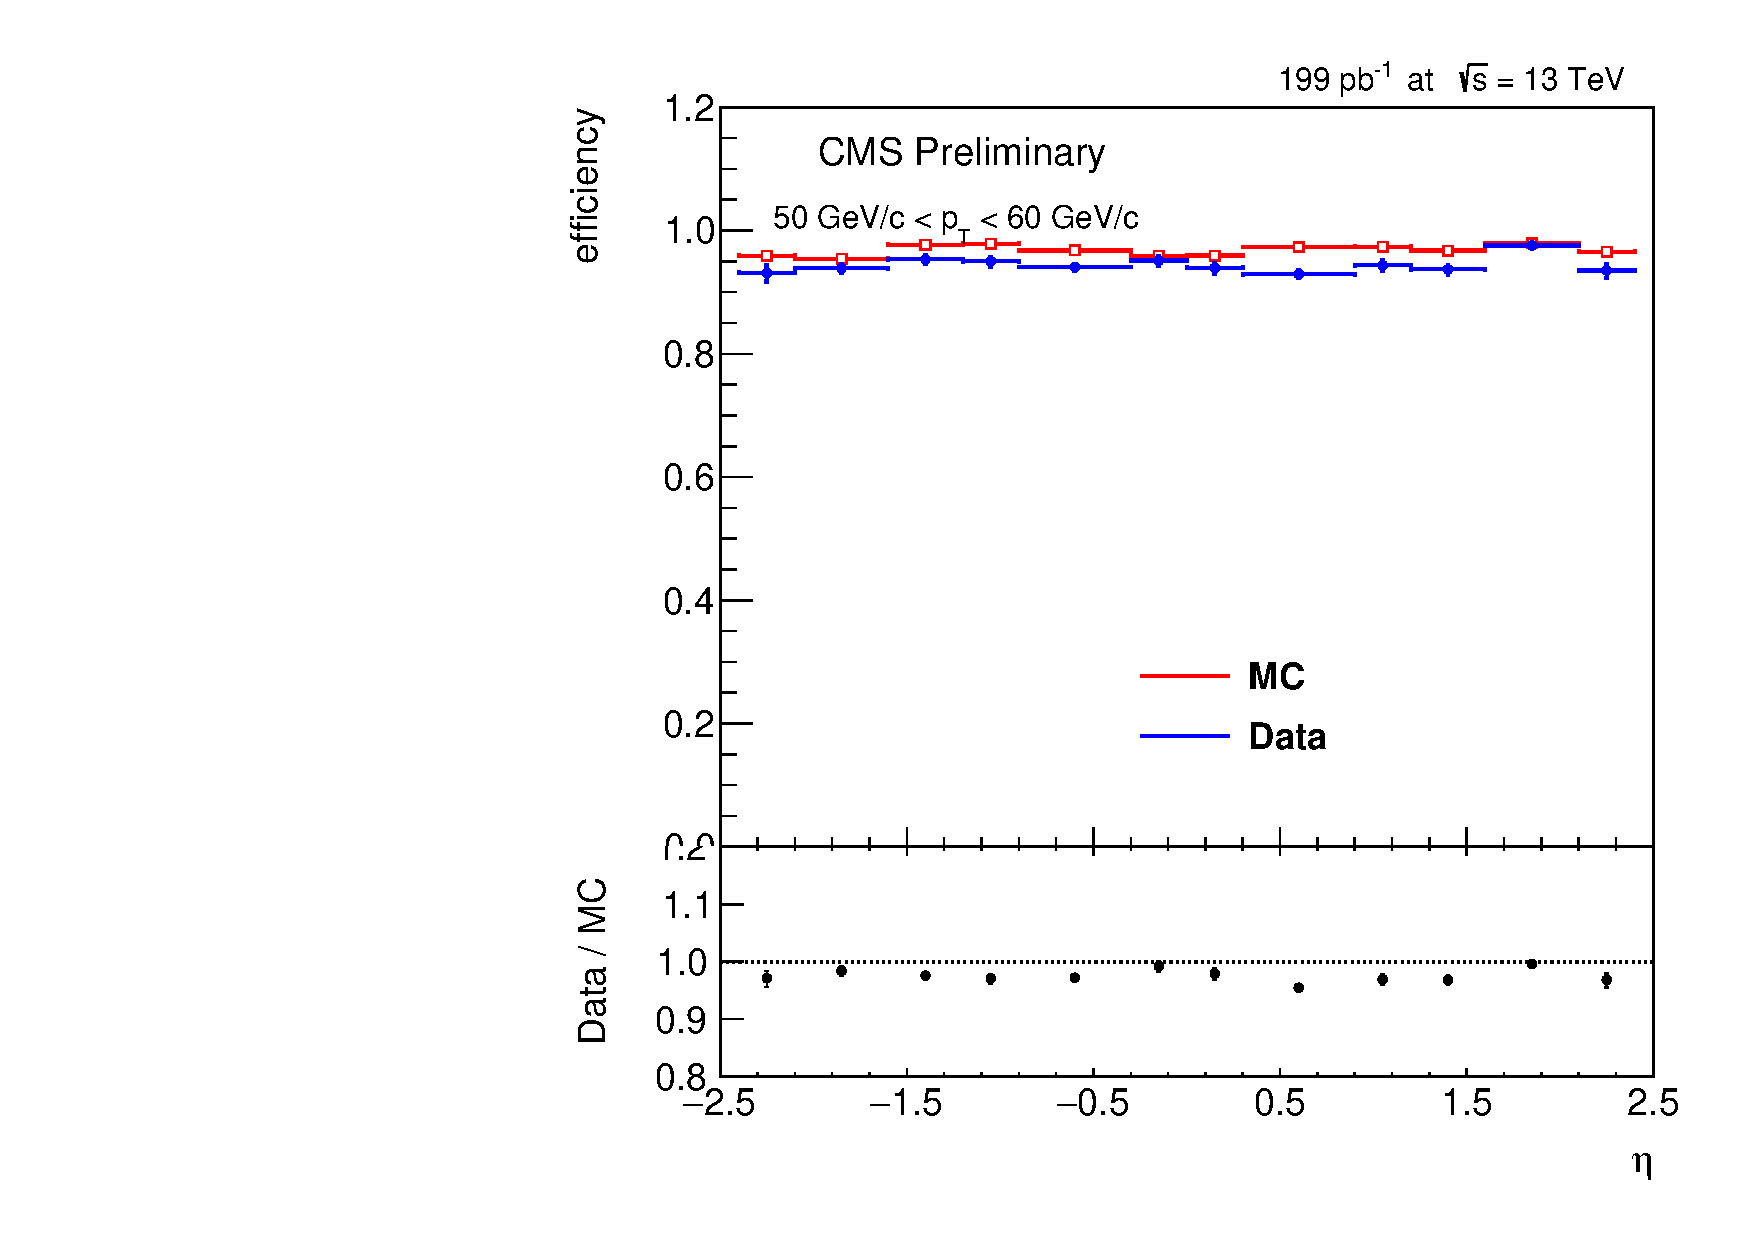
\includegraphics[width=0.32\linewidth]{plots/efficiency/13_zmmhlt_positive/PtBins_eta_pt9.pdf}
\caption{$\eta$ dependence of Single muon trigger efficiency scale factors, separated by $p_T$ bins, for positively charged muons in the 13 TeV samples.}
\label{fig:Eff:mu:13:HLT:pos}
\end{figure}
\begin{figure}
\centering
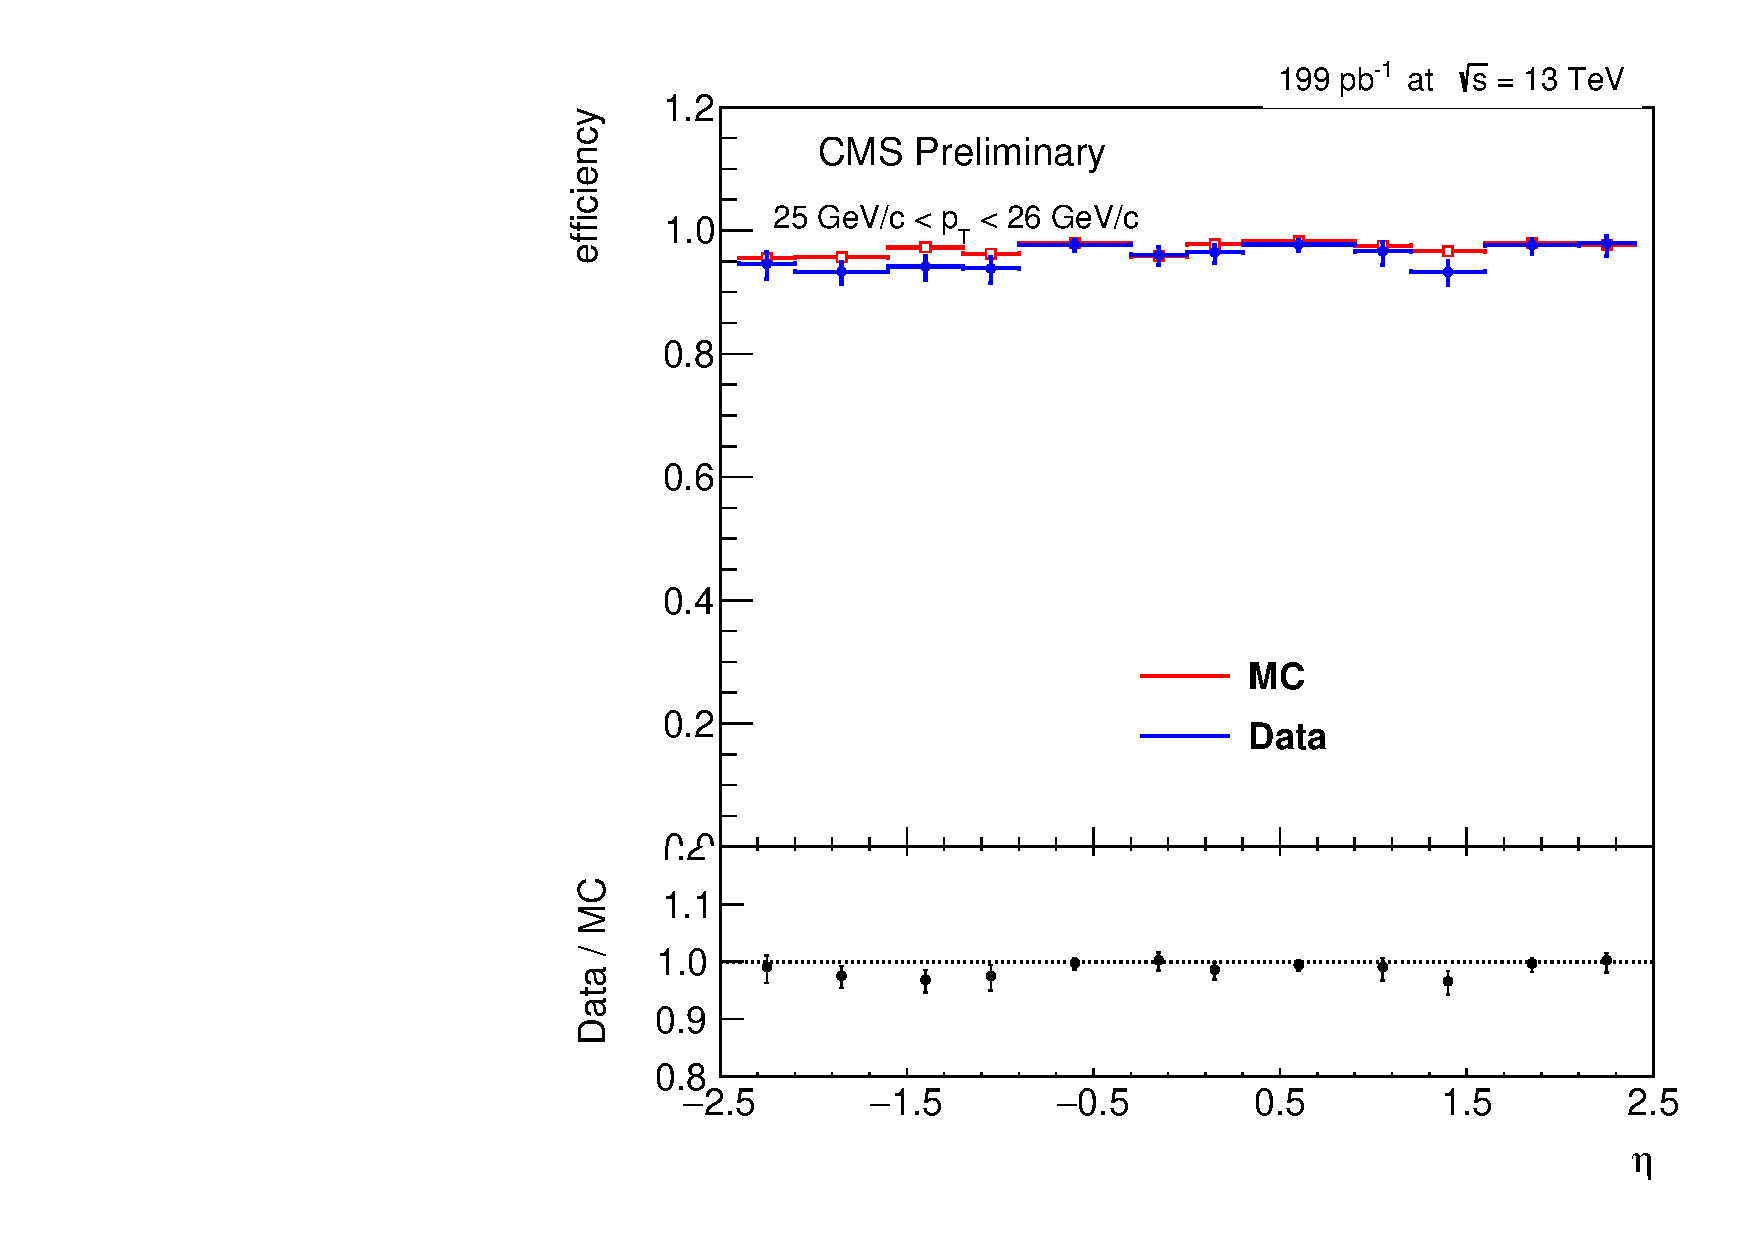
\includegraphics[width=0.32\linewidth]{plots/efficiency/13_zmmhlt_negative/PtBins_eta_pt0.pdf}
\includegraphics[width=0.32\linewidth]{plots/efficiency/13_zmmhlt_negative/PtBins_eta_pt1.pdf}
\includegraphics[width=0.32\linewidth]{plots/efficiency/13_zmmhlt_negative/PtBins_eta_pt10.pdf}
\includegraphics[width=0.32\linewidth]{plots/efficiency/13_zmmhlt_negative/PtBins_eta_pt11.pdf}
\includegraphics[width=0.32\linewidth]{plots/efficiency/13_zmmhlt_negative/PtBins_eta_pt2.pdf}
\includegraphics[width=0.32\linewidth]{plots/efficiency/13_zmmhlt_negative/PtBins_eta_pt3.pdf}
\includegraphics[width=0.32\linewidth]{plots/efficiency/13_zmmhlt_negative/PtBins_eta_pt4.pdf}
\includegraphics[width=0.32\linewidth]{plots/efficiency/13_zmmhlt_negative/PtBins_eta_pt5.pdf}
\includegraphics[width=0.32\linewidth]{plots/efficiency/13_zmmhlt_negative/PtBins_eta_pt6.pdf}
\includegraphics[width=0.32\linewidth]{plots/efficiency/13_zmmhlt_negative/PtBins_eta_pt7.pdf}
\includegraphics[width=0.32\linewidth]{plots/efficiency/13_zmmhlt_negative/PtBins_eta_pt8.pdf}
\includegraphics[width=0.32\linewidth]{plots/efficiency/13_zmmhlt_negative/PtBins_eta_pt9.pdf}
\caption{$\eta$ dependence of Single muon trigger efficiency scale factors, separated by $p_T$ bins, for negatively charged muons in the 13 TeV samples.}
\label{fig:Eff:mu:13:HLT:neg}
\end{figure}


%%%% Tables for EleGSFSel Efficiency  %%%%%
%% Efficiency table for ZeeGSFSel Combined
\begin{table}%[htbp]
\begin{center}
\scalebox{0.6}{
\begin{tabular}{ccccccc}
\hline
& $-2.4< \eta<-2$ & $-2< \eta<-1.566$ & $-1.566< \eta<-1.4442$ & $-1.4442< \eta<-1$ & $-1< \eta<-0.5$ & $-0.5< \eta<0$ \\
\hline \hline
$25<p_{T}<35$ & $0.959 \pm 0.018$ & $0.904 \pm 0.009$ & $0.885 \pm 0.052$ & $0.863 \pm 0.018$ & $0.855 \pm 0.013$ & $0.872 \pm 0.007$  \\
$35<p_{T}<50$ & $0.969 \pm 0.009$ & $0.934 \pm 0.009$ & $0.896 \pm 0.015$ & $0.904 \pm 0.005$ & $0.908 \pm 0.003$ & $0.905 \pm 0.004$  \\
$50<p_{T}<1e+04$ & $0.955 \pm 0.017$ & $0.971 \pm 0.014$ & $1.014 \pm 0.037$ & $0.921 \pm 0.012$ & $0.925 \pm 0.008$ & $0.899 \pm 0.007$  \\
\hline
& $0< \eta<0.5$ & $0.5< \eta<1$ & $1< \eta<1.44$ & $1.44< \eta<1.57$ & $1.57< \eta<2$ & $2< \eta<2.4$ \\
\hline \hline
$25<p_{T}<35$ & $0.891 \pm 0.013$ & $0.902 \pm 0.013$ & $0.844 \pm 0.015$ & $0.943 \pm 0.045$ & $0.925 \pm 0.010$ & $0.922 \pm 0.020$  \\
$35<p_{T}<50$ & $0.917 \pm 0.005$ & $0.936 \pm 0.001$ & $0.941 \pm 0.001$ & $0.923 \pm 0.021$ & $0.948 \pm 0.007$ & $0.954 \pm 0.006$  \\
$50<p_{T}<1e+04$ & $0.919 \pm 0.009$ & $0.943 \pm 0.009$ & $0.956 \pm 0.012$ & $0.959 \pm 0.089$ & $0.949 \pm 0.054$ & $0.982 \pm 0.020$  \\
\hline
\end{tabular}}
\end{center}
\caption{GSF electron identification and isolation efficiency scale factors in ($p_T$, $\eta$) bins for combined charged electrons in the 13 TeV samples.}
\label{tab:Eff:el:13TeV:GSFSel:com}
\end{table}

%%%% Tables for EleHLT Efficiency  %%%%%
%% Efficiency table for ZeeHLT Positive
\begin{table}%[htbp]
\begin{center}
\scalebox{0.6}{
\begin{tabular}{ccccccc}
\hline
& $-2.4< \eta<-2$ & $-2< \eta<-1.566$ & $-1.566< \eta<-1.4442$ & $-1.4442< \eta<-1$ & $-1< \eta<-0.5$ & $-0.5< \eta<0$ \\
\hline \hline
$25<p_{T}<26.5$ & $0.664 \pm 0.058$ & $0.921 \pm 0.054$ & $0.959 \pm 0.112$ & $1.053 \pm 0.046$ & $0.964 \pm 0.036$ & $1.031 \pm 0.030$  \\
$26.5<p_{T}<28$ & $0.646 \pm 0.056$ & $0.928 \pm 0.043$ & $1.033 \pm 0.103$ & $0.976 \pm 0.041$ & $0.962 \pm 0.031$ & $0.933 \pm 0.032$  \\
$28<p_{T}<29.5$ & $0.754 \pm 0.055$ & $0.986 \pm 0.037$ & $1.004 \pm 0.101$ & $1.016 \pm 0.037$ & $0.948 \pm 0.030$ & $0.977 \pm 0.025$  \\
$29.5<p_{T}<31$ & $0.624 \pm 0.048$ & $0.959 \pm 0.034$ & $0.981 \pm 0.093$ & $0.990 \pm 0.034$ & $0.961 \pm 0.027$ & $0.987 \pm 0.022$  \\
$31<p_{T}<32.5$ & $0.725 \pm 0.042$ & $0.907 \pm 0.036$ & $0.942 \pm 0.078$ & $1.037 \pm 0.028$ & $0.996 \pm 0.020$ & $0.991 \pm 0.020$  \\
$32.5<p_{T}<35$ & $0.747 \pm 0.032$ & $0.959 \pm 0.023$ & $0.972 \pm 0.065$ & $0.976 \pm 0.022$ & $0.979 \pm 0.014$ & $0.971 \pm 0.014$  \\
$35<p_{T}<40$ & $0.811 \pm 0.020$ & $0.957 \pm 0.014$ & $0.987 \pm 0.038$ & $0.995 \pm 0.011$ & $0.982 \pm 0.008$ & $0.991 \pm 0.008$  \\
$40<p_{T}<45$ & $0.831 \pm 0.018$ & $0.986 \pm 0.011$ & $0.976 \pm 0.029$ & $0.996 \pm 0.009$ & $0.999 \pm 0.006$ & $0.978 \pm 0.007$  \\
$45<p_{T}<50$ & $0.875 \pm 0.020$ & $0.966 \pm 0.013$ & $1.030 \pm 0.033$ & $0.985 \pm 0.011$ & $0.984 \pm 0.008$ & $0.980 \pm 0.008$  \\
$50<p_{T}<60$ & $0.857 \pm 0.026$ & $0.986 \pm 0.015$ & $0.988 \pm 0.048$ & $1.008 \pm 0.012$ & $0.989 \pm 0.009$ & $0.988 \pm 0.010$  \\
$60<p_{T}<80$ & $0.889 \pm 0.035$ & $0.998 \pm 0.024$ & $1.051 \pm 0.056$ & $0.993 \pm 0.018$ & $0.992 \pm 0.014$ & $0.974 \pm 0.016$  \\
$80<p_{T}<1e+04$ & $1.033 \pm 0.039$ & $0.978 \pm 0.036$ & $1.009 \pm 0.105$ & $0.996 \pm 0.027$ & $0.976 \pm 0.025$ & $0.980 \pm 0.026$  \\
\hline
& $0< \eta<0.5$ & $0.5< \eta<1$ & $1< \eta<1.44$ & $1.44< \eta<1.57$ & $1.57< \eta<2$ & $2< \eta<2.4$ \\
\hline \hline
$25<p_{T}<26.5$ & $0.952 \pm 0.035$ & $0.940 \pm 0.036$ & $1.088 \pm 0.039$ & $1.052 \pm 0.134$ & $0.871 \pm 0.048$ & $0.658 \pm 0.067$  \\
$26.5<p_{T}<28$ & $1.005 \pm 0.030$ & $0.958 \pm 0.033$ & $0.989 \pm 0.043$ & $1.082 \pm 0.131$ & $0.898 \pm 0.044$ & $0.800 \pm 0.059$  \\
$28<p_{T}<29.5$ & $0.980 \pm 0.026$ & $0.995 \pm 0.026$ & $0.964 \pm 0.046$ & $0.872 \pm 0.126$ & $0.968 \pm 0.039$ & $0.622 \pm 0.056$  \\
$29.5<p_{T}<31$ & $0.992 \pm 0.021$ & $0.964 \pm 0.025$ & $0.939 \pm 0.040$ & $1.000 \pm 0.105$ & $0.935 \pm 0.036$ & $0.751 \pm 0.049$  \\
$31<p_{T}<32.5$ & $0.980 \pm 0.020$ & $0.976 \pm 0.021$ & $1.025 \pm 0.029$ & $1.010 \pm 0.085$ & $0.923 \pm 0.035$ & $0.666 \pm 0.053$  \\
$32.5<p_{T}<35$ & $0.976 \pm 0.014$ & $0.970 \pm 0.014$ & $1.016 \pm 0.021$ & $0.807 \pm 0.083$ & $0.946 \pm 0.023$ & $0.805 \pm 0.032$  \\
$35<p_{T}<40$ & $0.972 \pm 0.008$ & $0.976 \pm 0.008$ & $0.993 \pm 0.011$ & $0.975 \pm 0.037$ & $0.963 \pm 0.014$ & $0.814 \pm 0.021$  \\
$40<p_{T}<45$ & $0.978 \pm 0.007$ & $0.987 \pm 0.007$ & $0.991 \pm 0.009$ & $1.022 \pm 0.031$ & $0.974 \pm 0.011$ & $0.846 \pm 0.019$  \\
$45<p_{T}<50$ & $0.973 \pm 0.008$ & $0.986 \pm 0.008$ & $0.997 \pm 0.011$ & $0.963 \pm 0.040$ & $0.952 \pm 0.013$ & $0.866 \pm 0.022$  \\
$50<p_{T}<60$ & $0.998 \pm 0.009$ & $0.980 \pm 0.010$ & $1.019 \pm 0.012$ & $0.995 \pm 0.043$ & $0.968 \pm 0.016$ & $0.907 \pm 0.026$  \\
$60<p_{T}<80$ & $0.970 \pm 0.017$ & $0.987 \pm 0.014$ & $1.016 \pm 0.017$ & $0.937 \pm 0.074$ & $0.989 \pm 0.023$ & $0.956 \pm 0.035$  \\
$80<p_{T}<1e+04$ & $0.982 \pm 0.022$ & $0.978 \pm 0.027$ & $1.048 \pm 0.017$ & $1.096 \pm 0.082$ & $0.950 \pm 0.043$ & $0.967 \pm 0.055$  \\
\hline
\end{tabular}}
\end{center}
\caption{Single electron trigger efficiency scale factors in ($p_T$, $\eta$) bins for positively charged electrons in the 13 TeV samples.}
\label{tab:Eff:el:13TeV:HLT:pos}
\end{table}
%% Efficiency table for ZeeHLT Negative
\begin{table}%[htbp]
\begin{center}
\scalebox{0.6}{
\begin{tabular}{ccccccc}
\hline
& $-2.4< \eta<-2$ & $-2< \eta<-1.566$ & $-1.566< \eta<-1.4442$ & $-1.4442< \eta<-1$ & $-1< \eta<-0.5$ & $-0.5< \eta<0$ \\
\hline \hline
$25<p_{T}<26.5$ & $0.722 \pm 0.059$ & $0.895 \pm 0.053$ & $0.909 \pm 0.133$ & $0.992 \pm 0.050$ & $0.965 \pm 0.034$ & $0.996 \pm 0.032$  \\
$26.5<p_{T}<28$ & $0.736 \pm 0.060$ & $0.922 \pm 0.047$ & $0.920 \pm 0.141$ & $1.002 \pm 0.040$ & $1.005 \pm 0.029$ & $0.963 \pm 0.028$  \\
$28<p_{T}<29.5$ & $0.746 \pm 0.052$ & $0.897 \pm 0.043$ & $0.965 \pm 0.117$ & $1.034 \pm 0.031$ & $0.971 \pm 0.027$ & $0.972 \pm 0.025$  \\
$29.5<p_{T}<31$ & $0.716 \pm 0.049$ & $0.953 \pm 0.033$ & $0.890 \pm 0.095$ & $0.994 \pm 0.030$ & $0.970 \pm 0.024$ & $0.971 \pm 0.022$  \\
$31<p_{T}<32.5$ & $0.745 \pm 0.044$ & $0.921 \pm 0.034$ & $1.023 \pm 0.107$ & $1.060 \pm 0.026$ & $1.006 \pm 0.020$ & $0.980 \pm 0.021$  \\
$32.5<p_{T}<35$ & $0.814 \pm 0.033$ & $0.977 \pm 0.024$ & $0.989 \pm 0.062$ & $1.001 \pm 0.018$ & $0.984 \pm 0.014$ & $0.972 \pm 0.015$  \\
$35<p_{T}<40$ & $0.768 \pm 0.020$ & $0.955 \pm 0.014$ & $0.989 \pm 0.039$ & $0.978 \pm 0.012$ & $0.985 \pm 0.007$ & $0.968 \pm 0.008$  \\
$40<p_{T}<45$ & $0.826 \pm 0.018$ & $0.977 \pm 0.011$ & $0.940 \pm 0.038$ & $1.003 \pm 0.009$ & $0.986 \pm 0.007$ & $0.984 \pm 0.007$  \\
$45<p_{T}<50$ & $0.879 \pm 0.021$ & $0.974 \pm 0.012$ & $1.012 \pm 0.037$ & $0.988 \pm 0.011$ & $0.991 \pm 0.008$ & $0.997 \pm 0.008$  \\
$50<p_{T}<60$ & $0.900 \pm 0.025$ & $1.005 \pm 0.014$ & $1.038 \pm 0.037$ & $1.014 \pm 0.011$ & $0.996 \pm 0.009$ & $0.982 \pm 0.010$  \\
$60<p_{T}<80$ & $0.869 \pm 0.038$ & $0.954 \pm 0.025$ & $0.846 \pm 0.089$ & $1.022 \pm 0.017$ & $0.995 \pm 0.014$ & $0.982 \pm 0.015$  \\
$80<p_{T}<1e+04$ & $0.983 \pm 0.055$ & $1.005 \pm 0.026$ & $0.941 \pm 0.134$ & $0.945 \pm 0.038$ & $0.982 \pm 0.025$ & $0.996 \pm 0.022$  \\
\hline
& $0< \eta<0.5$ & $0.5< \eta<1$ & $1< \eta<1.44$ & $1.44< \eta<1.57$ & $1.57< \eta<2$ & $2< \eta<2.4$ \\
\hline \hline
$25<p_{T}<26.5$ & $0.955 \pm 0.037$ & $0.969 \pm 0.035$ & $0.967 \pm 0.050$ & $0.999 \pm 0.136$ & $0.911 \pm 0.050$ & $0.703 \pm 0.068$  \\
$26.5<p_{T}<28$ & $0.971 \pm 0.031$ & $1.033 \pm 0.033$ & $1.010 \pm 0.043$ & $0.958 \pm 0.118$ & $0.902 \pm 0.044$ & $0.673 \pm 0.059$  \\
$28<p_{T}<29.5$ & $0.973 \pm 0.026$ & $0.987 \pm 0.025$ & $1.020 \pm 0.038$ & $0.994 \pm 0.102$ & $0.978 \pm 0.038$ & $0.815 \pm 0.053$  \\
$29.5<p_{T}<31$ & $0.945 \pm 0.025$ & $0.946 \pm 0.027$ & $1.020 \pm 0.034$ & $0.978 \pm 0.121$ & $0.886 \pm 0.037$ & $0.701 \pm 0.055$  \\
$31<p_{T}<32.5$ & $0.999 \pm 0.021$ & $0.979 \pm 0.021$ & $1.015 \pm 0.033$ & $0.927 \pm 0.110$ & $0.982 \pm 0.032$ & $0.781 \pm 0.048$  \\
$32.5<p_{T}<35$ & $0.963 \pm 0.015$ & $0.992 \pm 0.015$ & $1.014 \pm 0.020$ & $1.008 \pm 0.061$ & $0.973 \pm 0.021$ & $0.764 \pm 0.033$  \\
$35<p_{T}<40$ & $0.975 \pm 0.008$ & $0.975 \pm 0.008$ & $1.002 \pm 0.011$ & $0.963 \pm 0.039$ & $0.957 \pm 0.013$ & $0.824 \pm 0.021$  \\
$40<p_{T}<45$ & $0.983 \pm 0.007$ & $0.979 \pm 0.007$ & $0.989 \pm 0.009$ & $1.019 \pm 0.029$ & $0.964 \pm 0.011$ & $0.864 \pm 0.018$  \\
$45<p_{T}<50$ & $0.978 \pm 0.008$ & $0.980 \pm 0.008$ & $0.984 \pm 0.012$ & $1.035 \pm 0.036$ & $0.969 \pm 0.013$ & $0.829 \pm 0.023$  \\
$50<p_{T}<60$ & $0.986 \pm 0.010$ & $0.999 \pm 0.010$ & $1.008 \pm 0.012$ & $1.015 \pm 0.042$ & $0.962 \pm 0.016$ & $0.913 \pm 0.024$  \\
$60<p_{T}<80$ & $0.984 \pm 0.014$ & $1.015 \pm 0.014$ & $1.017 \pm 0.017$ & $1.056 \pm 0.059$ & $0.949 \pm 0.022$ & $0.905 \pm 0.038$  \\
$80<p_{T}<1e+04$ & $0.962 \pm 0.028$ & $1.005 \pm 0.021$ & $1.032 \pm 0.026$ & $1.204 \pm 0.154$ & $1.008 \pm 0.033$ & $0.867 \pm 0.092$  \\
\hline
\end{tabular}}
\end{center}
\caption{Single electron trigger efficiency scale factors in ($p_T$, $\eta$) bins for negatively charged electrons in the 13 TeV samples.}
\label{tab:Eff:el:13TeV:HLT:neg}
\end{table}


%%%% Tables for MuSIT Efficiency  %%%%%
%% Efficiency table for ZmmSIT Combined
\begin{table}%[htbp]
\begin{center}
\scalebox{0.6}{
\begin{tabular}{ccccccc}
\hline
& $-2.4< \eta<-2.1$ & $-2.1< \eta<-1.6$ & $-1.6< \eta<-1.2$ & $-1.2< \eta<-0.9$ & $-0.9< \eta<-0.3$ & $-0.3< \eta<0$ \\
\hline \hline
$25<p_{T}<35$ & $0.993 \pm 0.006$ & $1.009 \pm 0.005$ & $0.998 \pm 0.006$ & $1.002 \pm 0.007$ & $0.993 \pm 0.004$ & $0.985 \pm 0.005$  \\
$35<p_{T}<50$ & $0.987 \pm 0.003$ & $0.996 \pm 0.002$ & $0.998 \pm 0.002$ & $0.990 \pm 0.002$ & $0.993 \pm 0.002$ & $0.988 \pm 0.002$  \\
$50<p_{T}<1e+04$ & $0.975 \pm 0.007$ & $0.992 \pm 0.007$ & $0.997 \pm 0.003$ & $0.992 \pm 0.005$ & $0.993 \pm 0.003$ & $0.992 \pm 0.005$  \\
\hline
& $0< \eta<0.3$ & $0.3< \eta<0.9$ & $0.9< \eta<1.2$ & $1.2< \eta<1.6$ & $1.6< \eta<2.1$ & $2.1< \eta<2.4$ \\
\hline \hline
$25<p_{T}<35$ & $0.989 \pm 0.006$ & $0.992 \pm 0.004$ & $0.984 \pm 0.007$ & $0.999 \pm 0.006$ & $1.005 \pm 0.005$ & $1.003 \pm 0.006$  \\
$35<p_{T}<50$ & $0.995 \pm 0.003$ & $0.992 \pm 0.002$ & $0.988 \pm 0.002$ & $0.997 \pm 0.002$ & $1.002 \pm 0.001$ & $0.994 \pm 0.002$  \\
$50<p_{T}<1e+04$ & $0.979 \pm 0.005$ & $0.992 \pm 0.003$ & $0.994 \pm 0.005$ & $0.987 \pm 0.003$ & $0.997 \pm 0.003$ & $0.989 \pm 0.006$  \\
\hline
\end{tabular}}
\end{center}
\caption{Muon selection efficiency scale factors in ($p_T$, $\eta$) bins for combined charged muons in the 13 TeV samples.}
\label{tab:Eff:mu:13TeV:SIT:com}
\end{table}

%%%% Tables for MuSta Efficiency  %%%%%
%% Efficiency table for ZmmSta Combined
\begin{table}%[htbp]
\begin{center}
\scalebox{0.6}{
\begin{tabular}{ccccccc}
\hline
& $-2.4< \eta<-2.1$ & $-2.1< \eta<-1.6$ & $-1.6< \eta<-1.2$ & $-1.2< \eta<-0.9$ & $-0.9< \eta<-0.3$ & $-0.3< \eta<0$ \\
\hline \hline
$25<p_{T}<35$ & $0.990 \pm 0.007$ & $0.991 \pm 0.004$ & $0.986 \pm 0.006$ & $0.997 \pm 0.034$ & $0.992 \pm 0.009$ & $0.991 \pm 0.014$  \\
$35<p_{T}<50$ & $0.994 \pm 0.002$ & $0.996 \pm 0.002$ & $0.998 \pm 0.002$ & $0.997 \pm 0.002$ & $0.998 \pm 0.001$ & $0.986 \pm 0.002$  \\
$50<p_{T}<1e+04$ & $0.996 \pm 0.013$ & $0.995 \pm 0.004$ & $0.995 \pm 0.004$ & $0.995 \pm 0.005$ & $0.997 \pm 0.003$ & $0.989 \pm 0.005$  \\
\hline
& $0< \eta<0.3$ & $0.3< \eta<0.9$ & $0.9< \eta<1.2$ & $1.2< \eta<1.6$ & $1.6< \eta<2.1$ & $2.1< \eta<2.4$ \\
\hline \hline
$25<p_{T}<35$ & $0.983 \pm 0.006$ & $0.988 \pm 0.014$ & $1.008 \pm 0.017$ & $1.009 \pm 0.005$ & $1.004 \pm 0.008$ & $0.994 \pm 0.001$  \\
$35<p_{T}<50$ & $0.988 \pm 0.002$ & $0.991 \pm 0.002$ & $0.995 \pm 0.000$ & $0.998 \pm 0.002$ & $0.998 \pm 0.002$ & $0.996 \pm 0.001$  \\
$50<p_{T}<1e+04$ & $0.981 \pm 0.005$ & $0.988 \pm 0.003$ & $0.995 \pm 0.004$ & $0.995 \pm 0.004$ & $0.997 \pm 0.003$ & $0.992 \pm 0.005$  \\
\hline
\end{tabular}}
\end{center}
\caption{Standalone muon identification efficiency scale factors in ($p_T$, $\eta$) bins for combined charged muons in the 13 TeV samples.}
\label{tab:Eff:mu:13TeV:Sta:com}
\end{table}

%%%% Tables for MuHLT Efficiency  %%%%%
%% Efficiency table for ZmmHLT Positive
\begin{table}%[htbp]
\begin{center}
\scalebox{0.6}{
\begin{tabular}{ccccccc}
\hline
& $-2.4< \eta<-2.1$ & $-2.1< \eta<-1.6$ & $-1.6< \eta<-1.2$ & $-1.2< \eta<-0.9$ & $-0.9< \eta<-0.3$ & $-0.3< \eta<0$ \\
\hline \hline
$25<p_{T}<26.5$ & $0.960 \pm 0.030$ & $0.999 \pm 0.017$ & $0.928 \pm 0.023$ & $0.984 \pm 0.021$ & $0.981 \pm 0.012$ & $0.981 \pm 0.017$  \\
$26.5<p_{T}<28$ & $0.984 \pm 0.023$ & $0.984 \pm 0.016$ & $0.967 \pm 0.016$ & $0.978 \pm 0.019$ & $0.988 \pm 0.011$ & $0.976 \pm 0.016$  \\
$28<p_{T}<29.5$ & $0.974 \pm 0.023$ & $0.965 \pm 0.017$ & $0.987 \pm 0.014$ & $0.987 \pm 0.015$ & $0.987 \pm 0.010$ & $0.985 \pm 0.013$  \\
$29.5<p_{T}<31$ & $0.946 \pm 0.025$ & $0.971 \pm 0.015$ & $0.975 \pm 0.015$ & $0.973 \pm 0.016$ & $0.977 \pm 0.010$ & $1.013 \pm 0.010$  \\
$31<p_{T}<32.5$ & $0.974 \pm 0.020$ & $0.993 \pm 0.013$ & $0.964 \pm 0.014$ & $0.979 \pm 0.015$ & $0.986 \pm 0.008$ & $0.980 \pm 0.013$  \\
$32.5<p_{T}<35$ & $0.979 \pm 0.014$ & $0.969 \pm 0.011$ & $0.967 \pm 0.011$ & $0.984 \pm 0.009$ & $0.993 \pm 0.006$ & $0.982 \pm 0.009$  \\
$35<p_{T}<40$ & $0.988 \pm 0.009$ & $0.978 \pm 0.006$ & $0.963 \pm 0.006$ & $0.973 \pm 0.006$ & $0.986 \pm 0.004$ & $0.991 \pm 0.005$  \\
$40<p_{T}<45$ & $0.970 \pm 0.009$ & $0.972 \pm 0.006$ & $0.963 \pm 0.005$ & $0.972 \pm 0.005$ & $0.986 \pm 0.003$ & $0.990 \pm 0.005$  \\
$45<p_{T}<50$ & $0.947 \pm 0.012$ & $0.980 \pm 0.006$ & $0.968 \pm 0.006$ & $0.967 \pm 0.007$ & $0.986 \pm 0.004$ & $0.989 \pm 0.007$  \\
$50<p_{T}<60$ & $0.971 \pm 0.014$ & $0.984 \pm 0.009$ & $0.976 \pm 0.007$ & $0.971 \pm 0.008$ & $0.972 \pm 0.006$ & $0.992 \pm 0.009$  \\
$60<p_{T}<80$ & $1.004 \pm 0.023$ & $0.979 \pm 0.014$ & $0.962 \pm 0.013$ & $0.973 \pm 0.014$ & $0.988 \pm 0.009$ & $0.983 \pm 0.013$  \\
$80<p_{T}<1e+04$ & $0.951 \pm 0.082$ & $1.010 \pm 0.026$ & $0.949 \pm 0.026$ & $0.901 \pm 0.034$ & $0.953 \pm 0.020$ & $0.966 \pm 0.025$  \\
\hline
& $0< \eta<0.3$ & $0.3< \eta<0.9$ & $0.9< \eta<1.2$ & $1.2< \eta<1.6$ & $1.6< \eta<2.1$ & $2.1< \eta<2.4$ \\
\hline \hline
$25<p_{T}<26.5$ & $0.955 \pm 0.020$ & $0.981 \pm 0.012$ & $0.979 \pm 0.020$ & $0.960 \pm 0.020$ & $1.007 \pm 0.011$ & $0.993 \pm 0.023$  \\
$26.5<p_{T}<28$ & $1.004 \pm 0.014$ & $0.963 \pm 0.012$ & $0.958 \pm 0.021$ & $0.944 \pm 0.021$ & $1.001 \pm 0.012$ & $0.988 \pm 0.023$  \\
$28<p_{T}<29.5$ & $0.997 \pm 0.013$ & $0.966 \pm 0.011$ & $0.984 \pm 0.014$ & $0.987 \pm 0.015$ & $0.985 \pm 0.012$ & $0.972 \pm 0.021$  \\
$29.5<p_{T}<31$ & $0.979 \pm 0.013$ & $0.964 \pm 0.010$ & $0.939 \pm 0.019$ & $0.972 \pm 0.016$ & $0.984 \pm 0.011$ & $0.992 \pm 0.017$  \\
$31<p_{T}<32.5$ & $0.969 \pm 0.013$ & $0.969 \pm 0.009$ & $0.959 \pm 0.016$ & $0.961 \pm 0.015$ & $0.990 \pm 0.010$ & $1.001 \pm 0.017$  \\
$32.5<p_{T}<35$ & $0.987 \pm 0.009$ & $0.970 \pm 0.006$ & $0.957 \pm 0.012$ & $0.988 \pm 0.009$ & $0.983 \pm 0.008$ & $0.987 \pm 0.013$  \\
$35<p_{T}<40$ & $0.982 \pm 0.006$ & $0.967 \pm 0.004$ & $0.961 \pm 0.006$ & $0.968 \pm 0.006$ & $0.982 \pm 0.005$ & $0.998 \pm 0.007$  \\
$40<p_{T}<45$ & $0.979 \pm 0.005$ & $0.976 \pm 0.003$ & $0.972 \pm 0.005$ & $0.972 \pm 0.005$ & $0.985 \pm 0.004$ & $0.985 \pm 0.007$  \\
$45<p_{T}<50$ & $0.971 \pm 0.007$ & $0.968 \pm 0.005$ & $0.957 \pm 0.007$ & $0.976 \pm 0.006$ & $0.986 \pm 0.005$ & $0.981 \pm 0.010$  \\
$50<p_{T}<60$ & $0.979 \pm 0.009$ & $0.955 \pm 0.006$ & $0.969 \pm 0.009$ & $0.968 \pm 0.008$ & $0.996 \pm 0.005$ & $0.968 \pm 0.012$  \\
$60<p_{T}<80$ & $0.957 \pm 0.015$ & $0.978 \pm 0.008$ & $0.940 \pm 0.016$ & $0.998 \pm 0.010$ & $0.993 \pm 0.009$ & $0.969 \pm 0.023$  \\
$80<p_{T}<1e+04$ & $0.990 \pm 0.024$ & $0.974 \pm 0.017$ & $0.924 \pm 0.032$ & $0.948 \pm 0.027$ & $0.996 \pm 0.020$ & $0.960 \pm 0.048$  \\
\hline
\end{tabular}}
\end{center}
\caption{Single muon trigger efficiency scale factors in ($p_T$, $\eta$) bins for positively charged muons in the 13 TeV samples.}
\label{tab:Eff:mu:13TeV:HLT:pos}
\end{table}
%% Efficiency table for ZmmHLT Negative
\begin{table}%[htbp]
\begin{center}
\scalebox{0.6}{
\begin{tabular}{ccccccc}
\hline
& $-2.4< \eta<-2.1$ & $-2.1< \eta<-1.6$ & $-1.6< \eta<-1.2$ & $-1.2< \eta<-0.9$ & $-0.9< \eta<-0.3$ & $-0.3< \eta<0$ \\
\hline \hline
$25<p_{T}<26.5$ & $0.990 \pm 0.024$ & $0.975 \pm 0.019$ & $0.968 \pm 0.020$ & $0.975 \pm 0.022$ & $0.997 \pm 0.010$ & $1.002 \pm 0.016$  \\
$26.5<p_{T}<28$ & $0.983 \pm 0.023$ & $0.962 \pm 0.019$ & $0.944 \pm 0.020$ & $0.981 \pm 0.018$ & $0.969 \pm 0.011$ & $0.968 \pm 0.017$  \\
$28<p_{T}<29.5$ & $1.016 \pm 0.021$ & $0.968 \pm 0.017$ & $0.957 \pm 0.018$ & $0.966 \pm 0.017$ & $0.963 \pm 0.010$ & $1.004 \pm 0.011$  \\
$29.5<p_{T}<31$ & $0.968 \pm 0.022$ & $0.980 \pm 0.015$ & $0.966 \pm 0.015$ & $0.979 \pm 0.016$ & $0.980 \pm 0.008$ & $0.989 \pm 0.012$  \\
$31<p_{T}<32.5$ & $0.981 \pm 0.021$ & $0.994 \pm 0.013$ & $0.958 \pm 0.014$ & $0.980 \pm 0.013$ & $0.976 \pm 0.008$ & $0.994 \pm 0.011$  \\
$32.5<p_{T}<35$ & $0.947 \pm 0.016$ & $0.968 \pm 0.011$ & $0.965 \pm 0.011$ & $0.972 \pm 0.010$ & $0.988 \pm 0.005$ & $0.993 \pm 0.008$  \\
$35<p_{T}<40$ & $0.969 \pm 0.010$ & $0.973 \pm 0.006$ & $0.968 \pm 0.006$ & $0.975 \pm 0.006$ & $0.987 \pm 0.003$ & $0.989 \pm 0.005$  \\
$40<p_{T}<45$ & $0.971 \pm 0.009$ & $0.976 \pm 0.006$ & $0.970 \pm 0.005$ & $0.976 \pm 0.005$ & $0.981 \pm 0.003$ & $0.987 \pm 0.005$  \\
$45<p_{T}<50$ & $0.962 \pm 0.012$ & $0.977 \pm 0.007$ & $0.972 \pm 0.006$ & $0.978 \pm 0.006$ & $0.986 \pm 0.004$ & $0.991 \pm 0.006$  \\
$50<p_{T}<60$ & $0.957 \pm 0.015$ & $0.965 \pm 0.009$ & $0.972 \pm 0.008$ & $0.980 \pm 0.008$ & $0.975 \pm 0.006$ & $0.971 \pm 0.009$  \\
$60<p_{T}<80$ & $0.941 \pm 0.025$ & $0.956 \pm 0.015$ & $0.982 \pm 0.011$ & $0.969 \pm 0.014$ & $1.000 \pm 0.007$ & $1.006 \pm 0.011$  \\
$80<p_{T}<1e+04$ & $0.940 \pm 0.057$ & $0.965 \pm 0.028$ & $0.917 \pm 0.031$ & $0.957 \pm 0.028$ & $0.965 \pm 0.016$ & $0.986 \pm 0.026$  \\
\hline
& $0< \eta<0.3$ & $0.3< \eta<0.9$ & $0.9< \eta<1.2$ & $1.2< \eta<1.6$ & $1.6< \eta<2.1$ & $2.1< \eta<2.4$ \\
\hline \hline
$25<p_{T}<26.5$ & $0.986 \pm 0.015$ & $0.994 \pm 0.009$ & $0.991 \pm 0.020$ & $0.966 \pm 0.020$ & $0.997 \pm 0.012$ & $1.002 \pm 0.017$  \\
$26.5<p_{T}<28$ & $0.986 \pm 0.014$ & $0.986 \pm 0.010$ & $0.967 \pm 0.020$ & $0.951 \pm 0.021$ & $0.987 \pm 0.013$ & $0.994 \pm 0.023$  \\
$28<p_{T}<29.5$ & $0.966 \pm 0.015$ & $0.993 \pm 0.010$ & $0.993 \pm 0.014$ & $0.938 \pm 0.020$ & $0.997 \pm 0.010$ & $0.996 \pm 0.020$  \\
$29.5<p_{T}<31$ & $0.967 \pm 0.015$ & $0.986 \pm 0.009$ & $0.989 \pm 0.014$ & $0.961 \pm 0.017$ & $0.995 \pm 0.010$ & $0.993 \pm 0.017$  \\
$31<p_{T}<32.5$ & $0.992 \pm 0.012$ & $0.982 \pm 0.008$ & $0.972 \pm 0.014$ & $0.927 \pm 0.018$ & $0.990 \pm 0.010$ & $1.004 \pm 0.016$  \\
$32.5<p_{T}<35$ & $0.985 \pm 0.008$ & $0.993 \pm 0.005$ & $0.969 \pm 0.010$ & $0.964 \pm 0.010$ & $0.991 \pm 0.007$ & $0.992 \pm 0.012$  \\
$35<p_{T}<40$ & $0.978 \pm 0.006$ & $0.973 \pm 0.004$ & $0.969 \pm 0.006$ & $0.965 \pm 0.006$ & $0.994 \pm 0.004$ & $0.995 \pm 0.007$  \\
$40<p_{T}<45$ & $0.983 \pm 0.005$ & $0.981 \pm 0.003$ & $0.965 \pm 0.006$ & $0.974 \pm 0.005$ & $0.991 \pm 0.004$ & $0.985 \pm 0.007$  \\
$45<p_{T}<50$ & $0.981 \pm 0.007$ & $0.975 \pm 0.005$ & $0.957 \pm 0.008$ & $0.971 \pm 0.006$ & $0.988 \pm 0.005$ & $0.977 \pm 0.009$  \\
$50<p_{T}<60$ & $0.983 \pm 0.009$ & $0.974 \pm 0.006$ & $0.971 \pm 0.009$ & $0.975 \pm 0.008$ & $0.994 \pm 0.006$ & $0.990 \pm 0.012$  \\
$60<p_{T}<80$ & $1.003 \pm 0.013$ & $0.980 \pm 0.009$ & $0.942 \pm 0.016$ & $0.984 \pm 0.011$ & $0.995 \pm 0.009$ & $0.954 \pm 0.023$  \\
$80<p_{T}<1e+04$ & $0.944 \pm 0.031$ & $0.962 \pm 0.018$ & $0.981 \pm 0.023$ & $0.993 \pm 0.021$ & $1.001 \pm 0.019$ & $1.024 \pm 0.038$  \\
\hline
\end{tabular}}
\end{center}
\caption{Single muon trigger efficiency scale factors in ($p_T$, $\eta$) bins for negatively charged muons in the 13 TeV samples.}
\label{tab:Eff:mu:13TeV:HLT:neg}
\end{table}


%%%% Figures for EleGSFSel Efficiency  %%%%%
\begin{figure}
\centering
\includegraphics[width=0.32\linewidth]{plots/efficiency/5_zeegsfsel_combined/PtBins_eta_pt0.pdf}
\includegraphics[width=0.32\linewidth]{plots/efficiency/5_zeegsfsel_combined/PtBins_eta_pt1.pdf}
\includegraphics[width=0.32\linewidth]{plots/efficiency/5_zeegsfsel_combined/PtBins_eta_pt2.pdf}
\caption{$\eta$ dependence of GSF electron identification and isolation efficiency scale factors, separated by $p_T$ bins, for combined charged electrons in the 5 TeV samples.}
\label{fig:Eff:el:5:GSFSel:com}
\end{figure}

%%%% Figures for EleHLT Efficiency  %%%%%
\begin{figure}
\centering
\includegraphics[width=0.32\linewidth]{plots/efficiency/5_zeehlt_positive/PtBins_eta_pt0.pdf}
\includegraphics[width=0.32\linewidth]{plots/efficiency/5_zeehlt_positive/PtBins_eta_pt1.pdf}
\includegraphics[width=0.32\linewidth]{plots/efficiency/5_zeehlt_positive/PtBins_eta_pt10.pdf}
\includegraphics[width=0.32\linewidth]{plots/efficiency/5_zeehlt_positive/PtBins_eta_pt11.pdf}
\includegraphics[width=0.32\linewidth]{plots/efficiency/5_zeehlt_positive/PtBins_eta_pt2.pdf}
\includegraphics[width=0.32\linewidth]{plots/efficiency/5_zeehlt_positive/PtBins_eta_pt3.pdf}
\includegraphics[width=0.32\linewidth]{plots/efficiency/5_zeehlt_positive/PtBins_eta_pt4.pdf}
\includegraphics[width=0.32\linewidth]{plots/efficiency/5_zeehlt_positive/PtBins_eta_pt5.pdf}
\includegraphics[width=0.32\linewidth]{plots/efficiency/5_zeehlt_positive/PtBins_eta_pt6.pdf}
\includegraphics[width=0.32\linewidth]{plots/efficiency/5_zeehlt_positive/PtBins_eta_pt7.pdf}
\includegraphics[width=0.32\linewidth]{plots/efficiency/5_zeehlt_positive/PtBins_eta_pt8.pdf}
\includegraphics[width=0.32\linewidth]{plots/efficiency/5_zeehlt_positive/PtBins_eta_pt9.pdf}
\caption{$\eta$ dependence of Single electron trigger efficiency scale factors, separated by $p_T$ bins, for positively charged electrons in the 5 TeV samples.}
\label{fig:Eff:el:5:HLT:pos}
\end{figure}
\begin{figure}
\centering
\includegraphics[width=0.32\linewidth]{plots/efficiency/5_zeehlt_negative/PtBins_eta_pt0.pdf}
\includegraphics[width=0.32\linewidth]{plots/efficiency/5_zeehlt_negative/PtBins_eta_pt1.pdf}
\includegraphics[width=0.32\linewidth]{plots/efficiency/5_zeehlt_negative/PtBins_eta_pt10.pdf}
\includegraphics[width=0.32\linewidth]{plots/efficiency/5_zeehlt_negative/PtBins_eta_pt11.pdf}
\includegraphics[width=0.32\linewidth]{plots/efficiency/5_zeehlt_negative/PtBins_eta_pt2.pdf}
\includegraphics[width=0.32\linewidth]{plots/efficiency/5_zeehlt_negative/PtBins_eta_pt3.pdf}
\includegraphics[width=0.32\linewidth]{plots/efficiency/5_zeehlt_negative/PtBins_eta_pt4.pdf}
\includegraphics[width=0.32\linewidth]{plots/efficiency/5_zeehlt_negative/PtBins_eta_pt5.pdf}
\includegraphics[width=0.32\linewidth]{plots/efficiency/5_zeehlt_negative/PtBins_eta_pt6.pdf}
\includegraphics[width=0.32\linewidth]{plots/efficiency/5_zeehlt_negative/PtBins_eta_pt7.pdf}
\includegraphics[width=0.32\linewidth]{plots/efficiency/5_zeehlt_negative/PtBins_eta_pt8.pdf}
\includegraphics[width=0.32\linewidth]{plots/efficiency/5_zeehlt_negative/PtBins_eta_pt9.pdf}
\caption{$\eta$ dependence of Single electron trigger efficiency scale factors, separated by $p_T$ bins, for negatively charged electrons in the 5 TeV samples.}
\label{fig:Eff:el:5:HLT:neg}
\end{figure}


%%%% Figures for MuSIT Efficiency  %%%%%
\begin{figure}
\centering
\includegraphics[width=0.32\linewidth]{plots/efficiency/5_zmmsit_combined/PtBins_eta_pt0.pdf}
\includegraphics[width=0.32\linewidth]{plots/efficiency/5_zmmsit_combined/PtBins_eta_pt1.pdf}
\includegraphics[width=0.32\linewidth]{plots/efficiency/5_zmmsit_combined/PtBins_eta_pt2.pdf}
\caption{$\eta$ dependence of Muon selection efficiency scale factors, separated by $p_T$ bins, for combined charged muons in the 5 TeV samples.}
\label{fig:Eff:mu:5:SIT:com}
\end{figure}

%%%% Figures for MuSta Efficiency  %%%%%
\begin{figure}
\centering
\includegraphics[width=0.48\linewidth]{plots/efficiency/5_zmmsta_combined/PtBins_eta_pt0.pdf}
\includegraphics[width=0.48\linewidth]{plots/efficiency/5_zmmsta_combined/PtBins_eta_pt1.pdf}
\includegraphics[width=0.48\linewidth]{plots/efficiency/5_zmmsta_combined/PtBins_eta_pt2.pdf}
\caption{$\eta$ dependence of Standalone muon identification efficiency scale factors, separated by $p_T$ bins, for combined charged muons in the 5 TeV samples.}
\label{fig:Eff:mu:5:Sta:com}
\end{figure}

%%%% Figures for MuHLT Efficiency  %%%%%
\begin{figure}
\centering
\includegraphics[width=0.32\linewidth]{plots/efficiency/5_zmmhlt_positive/PtBins_eta_pt0.pdf}
\includegraphics[width=0.32\linewidth]{plots/efficiency/5_zmmhlt_positive/PtBins_eta_pt1.pdf}
\includegraphics[width=0.32\linewidth]{plots/efficiency/5_zmmhlt_positive/PtBins_eta_pt10.pdf}
\includegraphics[width=0.32\linewidth]{plots/efficiency/5_zmmhlt_positive/PtBins_eta_pt11.pdf}
\includegraphics[width=0.32\linewidth]{plots/efficiency/5_zmmhlt_positive/PtBins_eta_pt2.pdf}
\includegraphics[width=0.32\linewidth]{plots/efficiency/5_zmmhlt_positive/PtBins_eta_pt3.pdf}
\includegraphics[width=0.32\linewidth]{plots/efficiency/5_zmmhlt_positive/PtBins_eta_pt4.pdf}
\includegraphics[width=0.32\linewidth]{plots/efficiency/5_zmmhlt_positive/PtBins_eta_pt5.pdf}
\includegraphics[width=0.32\linewidth]{plots/efficiency/5_zmmhlt_positive/PtBins_eta_pt6.pdf}
\includegraphics[width=0.32\linewidth]{plots/efficiency/5_zmmhlt_positive/PtBins_eta_pt7.pdf}
\includegraphics[width=0.32\linewidth]{plots/efficiency/5_zmmhlt_positive/PtBins_eta_pt8.pdf}
\includegraphics[width=0.32\linewidth]{plots/efficiency/5_zmmhlt_positive/PtBins_eta_pt9.pdf}
\caption{$\eta$ dependence of Single muon trigger efficiency scale factors, separated by $p_T$ bins, for positively charged muons in the 5 TeV samples.}
\label{fig:Eff:mu:5:HLT:pos}
\end{figure}
\begin{figure}
\centering
\includegraphics[width=0.32\linewidth]{plots/efficiency/5_zmmhlt_negative/PtBins_eta_pt0.pdf}
\includegraphics[width=0.32\linewidth]{plots/efficiency/5_zmmhlt_negative/PtBins_eta_pt1.pdf}
\includegraphics[width=0.32\linewidth]{plots/efficiency/5_zmmhlt_negative/PtBins_eta_pt10.pdf}
\includegraphics[width=0.32\linewidth]{plots/efficiency/5_zmmhlt_negative/PtBins_eta_pt11.pdf}
\includegraphics[width=0.32\linewidth]{plots/efficiency/5_zmmhlt_negative/PtBins_eta_pt2.pdf}
\includegraphics[width=0.32\linewidth]{plots/efficiency/5_zmmhlt_negative/PtBins_eta_pt3.pdf}
\includegraphics[width=0.32\linewidth]{plots/efficiency/5_zmmhlt_negative/PtBins_eta_pt4.pdf}
\includegraphics[width=0.32\linewidth]{plots/efficiency/5_zmmhlt_negative/PtBins_eta_pt5.pdf}
\includegraphics[width=0.32\linewidth]{plots/efficiency/5_zmmhlt_negative/PtBins_eta_pt6.pdf}
\includegraphics[width=0.32\linewidth]{plots/efficiency/5_zmmhlt_negative/PtBins_eta_pt7.pdf}
\includegraphics[width=0.32\linewidth]{plots/efficiency/5_zmmhlt_negative/PtBins_eta_pt8.pdf}
\includegraphics[width=0.32\linewidth]{plots/efficiency/5_zmmhlt_negative/PtBins_eta_pt9.pdf}
\caption{$\eta$ dependence of Single muon trigger efficiency scale factors, separated by $p_T$ bins, for negatively charged muons in the 5 TeV samples.}
\label{fig:Eff:mu:5:HLT:neg}
\end{figure}


%%%% Tables for EleGSFSel Efficiency  %%%%%
%% Efficiency table for ZeeGSFSel Combined
\begin{table}%[htbp]
\begin{center}
\scalebox{0.6}{
\begin{tabular}{ccccccc}
\hline
& $-2.4< \eta<-2$ & $-2< \eta<-1.566$ & $-1.566< \eta<-1.4442$ & $-1.4442< \eta<-1$ & $-1< \eta<-0.5$ & $-0.5< \eta<0$ \\
\hline \hline
$25<p_{T}<35$ & $0.982 \pm 0.021$ & $0.911 \pm 0.012$ & $1.022 \pm 0.093$ & $0.905 \pm 0.023$ & $0.936 \pm 0.016$ & $0.947 \pm 0.011$  \\
$35<p_{T}<50$ & $0.974 \pm 0.010$ & $0.948 \pm 0.006$ & $0.939 \pm 0.020$ & $0.939 \pm 0.005$ & $0.947 \pm 0.005$ & $0.934 \pm 0.005$  \\
$50<p_{T}<1e+04$ & $0.981 \pm 0.021$ & $0.971 \pm 0.019$ & $0.991 \pm 0.043$ & $0.944 \pm 0.010$ & $0.958 \pm 0.011$ & $0.971 \pm 0.013$  \\
\hline
& $0< \eta<0.5$ & $0.5< \eta<1$ & $1< \eta<1.44$ & $1.44< \eta<1.57$ & $1.57< \eta<2$ & $2< \eta<2.4$ \\
\hline \hline
$25<p_{T}<35$ & $0.910 \pm 0.014$ & $0.925 \pm 0.017$ & $0.886 \pm 0.019$ & $0.873 \pm 0.043$ & $0.867 \pm 0.003$ & $0.966 \pm 0.023$  \\
$35<p_{T}<50$ & $0.934 \pm 0.004$ & $0.938 \pm 0.005$ & $0.925 \pm 0.008$ & $0.992 \pm 0.029$ & $0.945 \pm 0.006$ & $0.932 \pm 0.010$  \\
$50<p_{T}<1e+04$ & $0.932 \pm 0.008$ & $0.964 \pm 0.012$ & $0.955 \pm 0.010$ & $1.015 \pm 0.061$ & $0.953 \pm 0.017$ & $0.979 \pm 0.022$  \\
\hline
\end{tabular}}
\end{center}
\caption{GSF electron identification and isolation efficiency scale factors in ($p_T$, $\eta$) bins for combined charged electrons in the 5 TeV samples.}
\label{tab:Eff:el:5TeV:GSFSel:com}
\end{table}

%%%% Tables for EleHLT Efficiency  %%%%%
%% Efficiency table for ZeeHLT Positive
\begin{table}%[htbp]
\begin{center}
\scalebox{0.6}{
\begin{tabular}{ccccccc}
\hline
& $-2.4< \eta<-2$ & $-2< \eta<-1.566$ & $-1.566< \eta<-1.4442$ & $-1.4442< \eta<-1$ & $-1< \eta<-0.5$ & $-0.5< \eta<0$ \\
\hline \hline
$25<p_{T}<26.5$ & $0.530 \pm 0.086$ & $0.851 \pm 0.064$ & $0.713 \pm 0.266$ & $1.038 \pm 0.063$ & $0.969 \pm 0.050$ & $0.930 \pm 0.049$  \\
$26.5<p_{T}<28$ & $0.629 \pm 0.077$ & $0.903 \pm 0.059$ & $0.721 \pm 0.184$ & $1.051 \pm 0.053$ & $0.955 \pm 0.044$ & $0.959 \pm 0.042$  \\
$28<p_{T}<29.5$ & $0.641 \pm 0.067$ & $0.915 \pm 0.055$ & $1.103 \pm 0.127$ & $1.018 \pm 0.048$ & $0.926 \pm 0.041$ & $0.971 \pm 0.033$  \\
$29.5<p_{T}<31$ & $0.603 \pm 0.066$ & $0.917 \pm 0.047$ & $0.893 \pm 0.143$ & $0.980 \pm 0.041$ & $0.948 \pm 0.032$ & $0.946 \pm 0.032$  \\
$31<p_{T}<32.5$ & $0.700 \pm 0.063$ & $0.927 \pm 0.047$ & $0.886 \pm 0.129$ & $0.949 \pm 0.045$ & $0.956 \pm 0.027$ & $0.969 \pm 0.028$  \\
$32.5<p_{T}<35$ & $0.686 \pm 0.044$ & $0.913 \pm 0.032$ & $0.862 \pm 0.102$ & $0.951 \pm 0.029$ & $0.927 \pm 0.021$ & $0.962 \pm 0.019$  \\
$35<p_{T}<40$ & $0.817 \pm 0.025$ & $0.934 \pm 0.018$ & $0.931 \pm 0.051$ & $0.960 \pm 0.015$ & $0.935 \pm 0.012$ & $0.965 \pm 0.011$  \\
$40<p_{T}<45$ & $0.818 \pm 0.023$ & $0.933 \pm 0.015$ & $0.968 \pm 0.037$ & $0.970 \pm 0.012$ & $0.955 \pm 0.010$ & $0.964 \pm 0.009$  \\
$45<p_{T}<50$ & $0.827 \pm 0.029$ & $0.942 \pm 0.018$ & $0.984 \pm 0.049$ & $0.988 \pm 0.013$ & $0.964 \pm 0.012$ & $0.953 \pm 0.012$  \\
$50<p_{T}<60$ & $0.868 \pm 0.036$ & $0.895 \pm 0.027$ & $0.999 \pm 0.066$ & $1.005 \pm 0.018$ & $0.941 \pm 0.017$ & $0.969 \pm 0.015$  \\
$60<p_{T}<80$ & $0.890 \pm 0.082$ & $0.955 \pm 0.040$ & $0.931 \pm 0.143$ & $0.993 \pm 0.027$ & $0.972 \pm 0.026$ & $0.967 \pm 0.028$  \\
$80<p_{T}<1e+04$ & $0.952 \pm 0.225$ & $0.987 \pm 0.066$ & $0.833 \pm 0.449$ & $1.030 \pm 0.055$ & $0.983 \pm 0.041$ & $0.924 \pm 0.070$  \\
\hline
& $0< \eta<0.5$ & $0.5< \eta<1$ & $1< \eta<1.44$ & $1.44< \eta<1.57$ & $1.57< \eta<2$ & $2< \eta<2.4$ \\
\hline \hline
$25<p_{T}<26.5$ & $0.885 \pm 0.051$ & $0.901 \pm 0.054$ & $1.099 \pm 0.056$ & $0.890 \pm 0.192$ & $0.814 \pm 0.074$ & $0.641 \pm 0.087$  \\
$26.5<p_{T}<28$ & $0.938 \pm 0.047$ & $0.951 \pm 0.044$ & $1.008 \pm 0.059$ & $0.872 \pm 0.165$ & $0.808 \pm 0.068$ & $0.666 \pm 0.080$  \\
$28<p_{T}<29.5$ & $0.984 \pm 0.032$ & $0.962 \pm 0.042$ & $0.961 \pm 0.057$ & $0.860 \pm 0.168$ & $0.846 \pm 0.057$ & $0.692 \pm 0.090$  \\
$29.5<p_{T}<31$ & $0.964 \pm 0.034$ & $0.977 \pm 0.033$ & $0.976 \pm 0.046$ & $1.220 \pm 0.320$ & $0.906 \pm 0.052$ & $0.724 \pm 0.074$  \\
$31<p_{T}<32.5$ & $0.955 \pm 0.028$ & $0.947 \pm 0.033$ & $0.952 \pm 0.045$ & $0.801 \pm 0.118$ & $0.897 \pm 0.049$ & $0.743 \pm 0.077$  \\
$32.5<p_{T}<35$ & $0.929 \pm 0.020$ & $0.934 \pm 0.021$ & $0.916 \pm 0.034$ & $0.954 \pm 0.096$ & $0.853 \pm 0.037$ & $0.699 \pm 0.048$  \\
$35<p_{T}<40$ & $0.969 \pm 0.011$ & $0.955 \pm 0.011$ & $0.958 \pm 0.016$ & $0.937 \pm 0.050$ & $0.916 \pm 0.019$ & $0.764 \pm 0.029$  \\
$40<p_{T}<45$ & $0.954 \pm 0.010$ & $0.951 \pm 0.010$ & $0.945 \pm 0.014$ & $0.946 \pm 0.045$ & $0.937 \pm 0.016$ & $0.796 \pm 0.026$  \\
$45<p_{T}<50$ & $0.954 \pm 0.012$ & $0.954 \pm 0.013$ & $0.990 \pm 0.015$ & $0.948 \pm 0.051$ & $0.893 \pm 0.021$ & $0.829 \pm 0.031$  \\
$50<p_{T}<60$ & $0.948 \pm 0.018$ & $0.956 \pm 0.017$ & $0.932 \pm 0.023$ & $0.996 \pm 0.066$ & $0.984 \pm 0.023$ & $0.947 \pm 0.037$  \\
$60<p_{T}<80$ & $0.943 \pm 0.029$ & $0.942 \pm 0.032$ & $1.013 \pm 0.027$ & $1.016 \pm 0.143$ & $1.021 \pm 0.037$ & $1.020 \pm 0.062$  \\
$80<p_{T}<1e+04$ & $0.888 \pm 0.063$ & $0.960 \pm 0.057$ & $1.055 \pm 0.061$ & $0.576 \pm 0.365$ & $0.979 \pm 0.078$ & $0.882 \pm 0.240$  \\
\hline
\end{tabular}}
\end{center}
\caption{Single electron trigger efficiency scale factors in ($p_T$, $\eta$) bins for positively charged electrons in the 5 TeV samples.}
\label{tab:Eff:el:5TeV:HLT:pos}
\end{table}
%% Efficiency table for ZeeHLT Negative
\begin{table}%[htbp]
\begin{center}
\scalebox{0.6}{
\begin{tabular}{ccccccc}
\hline
& $-2.4< \eta<-2$ & $-2< \eta<-1.566$ & $-1.566< \eta<-1.4442$ & $-1.4442< \eta<-1$ & $-1< \eta<-0.5$ & $-0.5< \eta<0$ \\
\hline \hline
$25<p_{T}<26.5$ & $0.771 \pm 0.079$ & $0.887 \pm 0.065$ & $1.130 \pm 0.178$ & $1.056 \pm 0.062$ & $0.948 \pm 0.047$ & $0.988 \pm 0.049$  \\
$26.5<p_{T}<28$ & $0.767 \pm 0.069$ & $0.804 \pm 0.068$ & $0.838 \pm 0.172$ & $0.914 \pm 0.065$ & $0.927 \pm 0.047$ & $1.005 \pm 0.039$  \\
$28<p_{T}<29.5$ & $0.542 \pm 0.069$ & $0.889 \pm 0.057$ & $1.221 \pm 0.111$ & $0.975 \pm 0.048$ & $0.914 \pm 0.037$ & $0.958 \pm 0.036$  \\
$29.5<p_{T}<31$ & $0.719 \pm 0.058$ & $0.831 \pm 0.057$ & $0.918 \pm 0.168$ & $0.981 \pm 0.049$ & $0.952 \pm 0.034$ & $0.921 \pm 0.034$  \\
$31<p_{T}<32.5$ & $0.810 \pm 0.054$ & $0.934 \pm 0.047$ & $1.007 \pm 0.112$ & $0.987 \pm 0.037$ & $0.967 \pm 0.028$ & $0.913 \pm 0.032$  \\
$32.5<p_{T}<35$ & $0.734 \pm 0.042$ & $0.925 \pm 0.032$ & $0.973 \pm 0.080$ & $0.981 \pm 0.026$ & $0.935 \pm 0.020$ & $0.950 \pm 0.020$  \\
$35<p_{T}<40$ & $0.729 \pm 0.026$ & $0.909 \pm 0.019$ & $0.872 \pm 0.052$ & $0.949 \pm 0.015$ & $0.936 \pm 0.011$ & $0.952 \pm 0.011$  \\
$40<p_{T}<45$ & $0.825 \pm 0.023$ & $0.946 \pm 0.014$ & $0.964 \pm 0.043$ & $0.985 \pm 0.011$ & $0.970 \pm 0.009$ & $0.957 \pm 0.010$  \\
$45<p_{T}<50$ & $0.820 \pm 0.028$ & $0.961 \pm 0.017$ & $0.973 \pm 0.050$ & $0.975 \pm 0.014$ & $0.968 \pm 0.011$ & $0.943 \pm 0.013$  \\
$50<p_{T}<60$ & $0.866 \pm 0.036$ & $0.925 \pm 0.023$ & $0.938 \pm 0.069$ & $0.938 \pm 0.021$ & $0.940 \pm 0.018$ & $0.948 \pm 0.017$  \\
$60<p_{T}<80$ & $0.973 \pm 0.056$ & $0.982 \pm 0.039$ & $1.081 \pm 0.091$ & $1.050 \pm 0.024$ & $0.957 \pm 0.030$ & $0.960 \pm 0.028$  \\
$80<p_{T}<1e+04$ & $0.950 \pm 0.159$ & $0.982 \pm 0.111$ & $0.628 \pm 0.327$ & $0.996 \pm 0.068$ & $0.964 \pm 0.062$ & $0.833 \pm 0.070$  \\
\hline
& $0< \eta<0.5$ & $0.5< \eta<1$ & $1< \eta<1.44$ & $1.44< \eta<1.57$ & $1.57< \eta<2$ & $2< \eta<2.4$ \\
\hline \hline
$25<p_{T}<26.5$ & $0.898 \pm 0.053$ & $0.877 \pm 0.061$ & $0.895 \pm 0.076$ & $0.985 \pm 0.170$ & $0.818 \pm 0.069$ & $0.697 \pm 0.089$  \\
$26.5<p_{T}<28$ & $0.951 \pm 0.042$ & $0.956 \pm 0.045$ & $1.008 \pm 0.059$ & $1.142 \pm 0.109$ & $0.937 \pm 0.057$ & $0.636 \pm 0.078$  \\
$28<p_{T}<29.5$ & $0.947 \pm 0.037$ & $0.991 \pm 0.038$ & $0.901 \pm 0.054$ & $0.840 \pm 0.176$ & $0.875 \pm 0.065$ & $0.656 \pm 0.071$  \\
$29.5<p_{T}<31$ & $0.963 \pm 0.032$ & $0.895 \pm 0.036$ & $0.981 \pm 0.048$ & $0.884 \pm 0.123$ & $0.881 \pm 0.054$ & $0.567 \pm 0.068$  \\
$31<p_{T}<32.5$ & $0.940 \pm 0.030$ & $0.970 \pm 0.032$ & $0.982 \pm 0.047$ & $1.033 \pm 0.129$ & $0.918 \pm 0.045$ & $0.675 \pm 0.061$  \\
$32.5<p_{T}<35$ & $0.935 \pm 0.021$ & $0.940 \pm 0.021$ & $1.004 \pm 0.026$ & $0.809 \pm 0.109$ & $0.906 \pm 0.035$ & $0.700 \pm 0.043$  \\
$35<p_{T}<40$ & $0.955 \pm 0.012$ & $0.942 \pm 0.012$ & $0.949 \pm 0.016$ & $0.920 \pm 0.050$ & $0.889 \pm 0.020$ & $0.798 \pm 0.029$  \\
$40<p_{T}<45$ & $0.943 \pm 0.010$ & $0.963 \pm 0.010$ & $0.955 \pm 0.014$ & $0.991 \pm 0.041$ & $0.923 \pm 0.016$ & $0.776 \pm 0.026$  \\
$45<p_{T}<50$ & $0.956 \pm 0.012$ & $0.955 \pm 0.013$ & $0.947 \pm 0.017$ & $1.003 \pm 0.048$ & $0.914 \pm 0.020$ & $0.829 \pm 0.032$  \\
$50<p_{T}<60$ & $0.976 \pm 0.016$ & $0.946 \pm 0.017$ & $0.969 \pm 0.022$ & $0.977 \pm 0.065$ & $0.922 \pm 0.026$ & $0.810 \pm 0.043$  \\
$60<p_{T}<80$ & $0.963 \pm 0.028$ & $0.988 \pm 0.025$ & $0.979 \pm 0.035$ & $1.017 \pm 0.105$ & $0.936 \pm 0.050$ & $0.989 \pm 0.056$  \\
$80<p_{T}<1e+04$ & $0.996 \pm 0.039$ & $1.068 \pm 0.033$ & $0.878 \pm 0.103$ & $0.785 \pm 0.315$ & $0.959 \pm 0.092$ & $0.819 \pm 0.197$  \\
\hline
\end{tabular}}
\end{center}
\caption{Single electron trigger efficiency scale factors in ($p_T$, $\eta$) bins for negatively charged electrons in the 5 TeV samples.}
\label{tab:Eff:el:5TeV:HLT:neg}
\end{table}


%%%% Tables for MuSIT Efficiency  %%%%%
%% Efficiency table for ZmmSIT Combined
\begin{table}%[htbp]
\begin{center}
\scalebox{0.6}{
\begin{tabular}{ccccccc}
\hline
& $-2.4< \eta<-2.1$ & $-2.1< \eta<-1.6$ & $-1.6< \eta<-1.2$ & $-1.2< \eta<-0.9$ & $-0.9< \eta<-0.3$ & $-0.3< \eta<0$ \\
\hline \hline
$25<p_{T}<35$ & $0.991 \pm 0.007$ & $1.003 \pm 0.005$ & $1.005 \pm 0.006$ & $0.992 \pm 0.007$ & $0.997 \pm 0.004$ & $0.990 \pm 0.006$  \\
$35<p_{T}<50$ & $0.991 \pm 0.003$ & $0.996 \pm 0.002$ & $0.999 \pm 0.002$ & $0.993 \pm 0.003$ & $0.996 \pm 0.002$ & $0.990 \pm 0.003$  \\
$50<p_{T}<1e+04$ & $0.978 \pm 0.008$ & $1.001 \pm 0.004$ & $0.989 \pm 0.005$ & $0.991 \pm 0.006$ & $0.991 \pm 0.004$ & $0.997 \pm 0.005$  \\
\hline
& $0< \eta<0.3$ & $0.3< \eta<0.9$ & $0.9< \eta<1.2$ & $1.2< \eta<1.6$ & $1.6< \eta<2.1$ & $2.1< \eta<2.4$ \\
\hline \hline
$25<p_{T}<35$ & $0.985 \pm 0.006$ & $0.999 \pm 0.005$ & $1.002 \pm 0.007$ & $0.995 \pm 0.006$ & $0.996 \pm 0.005$ & $0.995 \pm 0.007$  \\
$35<p_{T}<50$ & $0.992 \pm 0.003$ & $0.992 \pm 0.002$ & $0.986 \pm 0.002$ & $0.997 \pm 0.002$ & $0.996 \pm 0.002$ & $0.991 \pm 0.003$  \\
$50<p_{T}<1e+04$ & $0.992 \pm 0.007$ & $0.995 \pm 0.004$ & $0.990 \pm 0.006$ & $0.994 \pm 0.004$ & $1.002 \pm 0.004$ & $0.996 \pm 0.008$  \\
\hline
\end{tabular}}
\end{center}
\caption{Muon selection efficiency scale factors in ($p_T$, $\eta$) bins for combined charged muons in the 5 TeV samples.}
\label{tab:Eff:mu:5TeV:SIT:com}
\end{table}

%%%% Tables for MuSta Efficiency  %%%%%
%% Efficiency table for ZmmSta Combined
\begin{table}%[htbp]
\begin{center}
\scalebox{0.6}{
\begin{tabular}{ccccccc}
\hline
& $-2.4< \eta<-2.1$ & $-2.1< \eta<-1.6$ & $-1.6< \eta<-1.2$ & $-1.2< \eta<-0.9$ & $-0.9< \eta<-0.3$ & $-0.3< \eta<0$ \\
\hline \hline
$25<p_{T}<35$ & $0.990 \pm 0.008$ & $0.978 \pm 0.015$ & $0.992 \pm 0.000$ & $0.970 \pm 0.001$ & $1.003 \pm 0.006$ & $0.992 \pm 0.006$  \\
$35<p_{T}<50$ & $0.987 \pm 0.002$ & $0.992 \pm 0.000$ & $1.000 \pm 0.001$ & $0.996 \pm 0.001$ & $0.997 \pm 0.001$ & $0.993 \pm 0.001$  \\
$50<p_{T}<1e+04$ & $0.990 \pm 0.001$ & $0.984 \pm 0.007$ & $0.986 \pm 0.009$ & $1.000 \pm 0.003$ & $0.996 \pm 0.003$ & $0.990 \pm 0.006$  \\
\hline
& $0< \eta<0.3$ & $0.3< \eta<0.9$ & $0.9< \eta<1.2$ & $1.2< \eta<1.6$ & $1.6< \eta<2.1$ & $2.1< \eta<2.4$ \\
\hline \hline
$25<p_{T}<35$ & $0.980 \pm 0.007$ & $0.985 \pm 0.007$ & $0.994 \pm 0.011$ & $0.992 \pm 0.000$ & $0.963 \pm 0.020$ & $0.951 \pm 0.019$  \\
$35<p_{T}<50$ & $0.992 \pm 0.004$ & $0.996 \pm 0.000$ & $0.990 \pm 0.002$ & $0.993 \pm 0.000$ & $0.995 \pm 0.000$ & $0.995 \pm 0.001$  \\
$50<p_{T}<1e+04$ & $0.972 \pm 0.007$ & $0.997 \pm 0.002$ & $0.992 \pm 0.005$ & $0.981 \pm 0.008$ & $0.987 \pm 0.009$ & $0.995 \pm 0.006$  \\
\hline
\end{tabular}}
\end{center}
\caption{Standalone muon identification efficiency scale factors in ($p_T$, $\eta$) bins for combined charged muons in the 5 TeV samples.}
\label{tab:Eff:mu:5TeV:Sta:com}
\end{table}

%%%% Tables for MuHLT Efficiency  %%%%%
%% Efficiency table for ZmmHLT Positive
\begin{table}%[htbp]
\begin{center}
\scalebox{0.6}{
\begin{tabular}{ccccccc}
\hline
& $-2.4< \eta<-2.1$ & $-2.1< \eta<-1.6$ & $-1.6< \eta<-1.2$ & $-1.2< \eta<-0.9$ & $-0.9< \eta<-0.3$ & $-0.3< \eta<0$ \\
\hline \hline
$25<p_{T}<26.5$ & $0.974 \pm 0.041$ & $1.013 \pm 0.020$ & $1.023 \pm 0.015$ & $0.984 \pm 0.023$ & $1.014 \pm 0.011$ & $1.006 \pm 0.019$  \\
$26.5<p_{T}<28$ & $0.999 \pm 0.027$ & $0.992 \pm 0.022$ & $0.965 \pm 0.022$ & $0.946 \pm 0.031$ & $1.002 \pm 0.011$ & $0.988 \pm 0.019$  \\
$28<p_{T}<29.5$ & $0.971 \pm 0.030$ & $0.962 \pm 0.024$ & $0.995 \pm 0.016$ & $0.979 \pm 0.022$ & $0.981 \pm 0.013$ & $0.961 \pm 0.020$  \\
$29.5<p_{T}<31$ & $0.972 \pm 0.031$ & $0.992 \pm 0.017$ & $0.969 \pm 0.018$ & $0.986 \pm 0.018$ & $0.973 \pm 0.013$ & $0.998 \pm 0.015$  \\
$31<p_{T}<32.5$ & $0.970 \pm 0.028$ & $0.969 \pm 0.020$ & $0.986 \pm 0.017$ & $0.973 \pm 0.019$ & $0.979 \pm 0.011$ & $0.992 \pm 0.015$  \\
$32.5<p_{T}<35$ & $0.982 \pm 0.019$ & $0.995 \pm 0.011$ & $0.973 \pm 0.013$ & $0.990 \pm 0.011$ & $0.987 \pm 0.007$ & $0.976 \pm 0.011$  \\
$35<p_{T}<40$ & $1.001 \pm 0.010$ & $0.983 \pm 0.008$ & $0.976 \pm 0.007$ & $0.974 \pm 0.007$ & $0.995 \pm 0.004$ & $0.987 \pm 0.007$  \\
$40<p_{T}<45$ & $0.996 \pm 0.010$ & $0.983 \pm 0.006$ & $0.983 \pm 0.005$ & $0.972 \pm 0.006$ & $0.990 \pm 0.004$ & $0.998 \pm 0.006$  \\
$45<p_{T}<50$ & $0.997 \pm 0.014$ & $0.990 \pm 0.008$ & $0.984 \pm 0.006$ & $0.986 \pm 0.007$ & $0.995 \pm 0.005$ & $0.998 \pm 0.008$  \\
$50<p_{T}<60$ & $0.999 \pm 0.019$ & $0.989 \pm 0.011$ & $0.988 \pm 0.009$ & $0.972 \pm 0.012$ & $1.007 \pm 0.007$ & $0.983 \pm 0.012$  \\
$60<p_{T}<80$ & $0.971 \pm 0.043$ & $0.999 \pm 0.018$ & $0.955 \pm 0.021$ & $0.978 \pm 0.019$ & $0.995 \pm 0.013$ & $0.991 \pm 0.023$  \\
$80<p_{T}<1e+04$ & $0.979 \pm 0.182$ & $1.005 \pm 0.047$ & $0.969 \pm 0.040$ & $0.985 \pm 0.051$ & $1.000 \pm 0.028$ & $0.984 \pm 0.055$  \\
\hline
& $0< \eta<0.3$ & $0.3< \eta<0.9$ & $0.9< \eta<1.2$ & $1.2< \eta<1.6$ & $1.6< \eta<2.1$ & $2.1< \eta<2.4$ \\
\hline \hline
$25<p_{T}<26.5$ & $0.999 \pm 0.019$ & $0.959 \pm 0.017$ & $0.972 \pm 0.024$ & $0.983 \pm 0.022$ & $0.989 \pm 0.020$ & $0.954 \pm 0.035$  \\
$26.5<p_{T}<28$ & $0.977 \pm 0.020$ & $0.964 \pm 0.015$ & $0.937 \pm 0.032$ & $0.938 \pm 0.026$ & $1.003 \pm 0.016$ & $0.995 \pm 0.027$  \\
$28<p_{T}<29.5$ & $0.977 \pm 0.021$ & $0.975 \pm 0.013$ & $0.967 \pm 0.022$ & $0.973 \pm 0.021$ & $0.974 \pm 0.017$ & $0.993 \pm 0.028$  \\
$29.5<p_{T}<31$ & $1.000 \pm 0.014$ & $0.979 \pm 0.011$ & $0.920 \pm 0.027$ & $0.996 \pm 0.016$ & $0.981 \pm 0.016$ & $1.030 \pm 0.018$  \\
$31<p_{T}<32.5$ & $0.964 \pm 0.016$ & $0.970 \pm 0.012$ & $0.994 \pm 0.015$ & $0.978 \pm 0.017$ & $0.988 \pm 0.013$ & $0.948 \pm 0.029$  \\
$32.5<p_{T}<35$ & $0.978 \pm 0.011$ & $0.991 \pm 0.006$ & $0.957 \pm 0.014$ & $0.962 \pm 0.014$ & $0.979 \pm 0.010$ & $0.997 \pm 0.015$  \\
$35<p_{T}<40$ & $0.981 \pm 0.007$ & $0.980 \pm 0.004$ & $0.965 \pm 0.007$ & $0.964 \pm 0.008$ & $0.985 \pm 0.006$ & $0.983 \pm 0.010$  \\
$40<p_{T}<45$ & $0.987 \pm 0.006$ & $0.977 \pm 0.004$ & $0.965 \pm 0.006$ & $0.986 \pm 0.005$ & $0.989 \pm 0.005$ & $0.992 \pm 0.009$  \\
$45<p_{T}<50$ & $0.981 \pm 0.009$ & $0.968 \pm 0.006$ & $0.959 \pm 0.009$ & $0.972 \pm 0.008$ & $0.972 \pm 0.007$ & $0.997 \pm 0.011$  \\
$50<p_{T}<60$ & $0.970 \pm 0.013$ & $0.982 \pm 0.007$ & $0.967 \pm 0.012$ & $0.980 \pm 0.010$ & $0.988 \pm 0.008$ & $0.973 \pm 0.022$  \\
$60<p_{T}<80$ & $0.988 \pm 0.022$ & $0.964 \pm 0.016$ & $0.942 \pm 0.027$ & $0.975 \pm 0.020$ & $0.990 \pm 0.018$ & $0.970 \pm 0.036$  \\
$80<p_{T}<1e+04$ & $0.978 \pm 0.053$ & $0.993 \pm 0.025$ & $0.878 \pm 0.069$ & $0.869 \pm 0.071$ & $1.032 \pm 0.032$ & $1.000 \pm 0.094$  \\
\hline
\end{tabular}}
\end{center}
\caption{Single muon trigger efficiency scale factors in ($p_T$, $\eta$) bins for positively charged muons in the 5 TeV samples.}
\label{tab:Eff:mu:5TeV:HLT:pos}
\end{table}
%% Efficiency table for ZmmHLT Negative
\begin{table}%[htbp]
\begin{center}
\scalebox{0.6}{
\begin{tabular}{ccccccc}
\hline
& $-2.4< \eta<-2.1$ & $-2.1< \eta<-1.6$ & $-1.6< \eta<-1.2$ & $-1.2< \eta<-0.9$ & $-0.9< \eta<-0.3$ & $-0.3< \eta<0$ \\
\hline \hline
$25<p_{T}<26.5$ & $0.951 \pm 0.044$ & $0.981 \pm 0.024$ & $0.991 \pm 0.021$ & $0.974 \pm 0.024$ & $0.985 \pm 0.016$ & $1.003 \pm 0.016$  \\
$26.5<p_{T}<28$ & $0.972 \pm 0.039$ & $0.983 \pm 0.019$ & $1.002 \pm 0.016$ & $1.011 \pm 0.017$ & $0.975 \pm 0.014$ & $0.996 \pm 0.016$  \\
$28<p_{T}<29.5$ & $0.989 \pm 0.033$ & $0.998 \pm 0.018$ & $0.982 \pm 0.018$ & $0.954 \pm 0.023$ & $0.985 \pm 0.011$ & $0.974 \pm 0.019$  \\
$29.5<p_{T}<31$ & $0.985 \pm 0.033$ & $0.981 \pm 0.019$ & $0.984 \pm 0.018$ & $0.963 \pm 0.021$ & $0.977 \pm 0.011$ & $0.991 \pm 0.015$  \\
$31<p_{T}<32.5$ & $0.997 \pm 0.025$ & $0.999 \pm 0.016$ & $0.992 \pm 0.015$ & $0.973 \pm 0.019$ & $0.986 \pm 0.010$ & $1.012 \pm 0.011$  \\
$32.5<p_{T}<35$ & $1.009 \pm 0.016$ & $0.985 \pm 0.013$ & $0.988 \pm 0.011$ & $0.982 \pm 0.014$ & $0.979 \pm 0.007$ & $0.987 \pm 0.011$  \\
$35<p_{T}<40$ & $0.990 \pm 0.011$ & $0.982 \pm 0.007$ & $0.983 \pm 0.006$ & $0.966 \pm 0.008$ & $0.979 \pm 0.004$ & $0.970 \pm 0.007$  \\
$40<p_{T}<45$ & $0.995 \pm 0.010$ & $0.991 \pm 0.006$ & $0.986 \pm 0.005$ & $0.972 \pm 0.006$ & $0.978 \pm 0.004$ & $0.993 \pm 0.006$  \\
$45<p_{T}<50$ & $0.976 \pm 0.014$ & $0.992 \pm 0.007$ & $0.974 \pm 0.007$ & $0.984 \pm 0.008$ & $0.988 \pm 0.005$ & $0.981 \pm 0.008$  \\
$50<p_{T}<60$ & $0.986 \pm 0.018$ & $0.989 \pm 0.010$ & $0.991 \pm 0.009$ & $0.970 \pm 0.012$ & $0.994 \pm 0.007$ & $0.992 \pm 0.010$  \\
$60<p_{T}<80$ & $1.029 \pm 0.027$ & $0.968 \pm 0.021$ & $0.969 \pm 0.019$ & $0.978 \pm 0.020$ & $0.982 \pm 0.012$ & $1.000 \pm 0.020$  \\
$80<p_{T}<1e+04$ & $0.920 \pm 0.140$ & $1.008 \pm 0.038$ & $0.998 \pm 0.045$ & $0.969 \pm 0.054$ & $0.992 \pm 0.033$ & $1.003 \pm 0.041$  \\
\hline
& $0< \eta<0.3$ & $0.3< \eta<0.9$ & $0.9< \eta<1.2$ & $1.2< \eta<1.6$ & $1.6< \eta<2.1$ & $2.1< \eta<2.4$ \\
\hline \hline
$25<p_{T}<26.5$ & $0.994 \pm 0.021$ & $0.982 \pm 0.017$ & $0.961 \pm 0.029$ & $0.976 \pm 0.026$ & $1.003 \pm 0.014$ & $1.038 \pm 0.020$  \\
$26.5<p_{T}<28$ & $0.992 \pm 0.019$ & $0.975 \pm 0.015$ & $0.983 \pm 0.023$ & $0.953 \pm 0.024$ & $0.984 \pm 0.017$ & $0.990 \pm 0.030$  \\
$28<p_{T}<29.5$ & $1.007 \pm 0.015$ & $0.986 \pm 0.013$ & $0.969 \pm 0.024$ & $0.988 \pm 0.019$ & $0.993 \pm 0.014$ & $0.989 \pm 0.029$  \\
$29.5<p_{T}<31$ & $1.002 \pm 0.014$ & $0.994 \pm 0.010$ & $0.955 \pm 0.023$ & $1.003 \pm 0.016$ & $0.991 \pm 0.015$ & $0.974 \pm 0.028$  \\
$31<p_{T}<32.5$ & $0.999 \pm 0.014$ & $0.983 \pm 0.010$ & $0.974 \pm 0.017$ & $0.970 \pm 0.018$ & $0.969 \pm 0.016$ & $1.025 \pm 0.017$  \\
$32.5<p_{T}<35$ & $1.001 \pm 0.010$ & $0.978 \pm 0.008$ & $0.966 \pm 0.013$ & $0.979 \pm 0.012$ & $1.000 \pm 0.008$ & $0.968 \pm 0.019$  \\
$35<p_{T}<40$ & $0.984 \pm 0.007$ & $0.987 \pm 0.004$ & $0.969 \pm 0.007$ & $0.971 \pm 0.007$ & $0.988 \pm 0.006$ & $0.997 \pm 0.009$  \\
$40<p_{T}<45$ & $0.985 \pm 0.006$ & $0.977 \pm 0.004$ & $0.965 \pm 0.007$ & $0.971 \pm 0.006$ & $0.992 \pm 0.005$ & $0.986 \pm 0.009$  \\
$45<p_{T}<50$ & $0.988 \pm 0.008$ & $0.987 \pm 0.005$ & $0.965 \pm 0.009$ & $0.969 \pm 0.008$ & $1.000 \pm 0.005$ & $0.987 \pm 0.012$  \\
$50<p_{T}<60$ & $1.000 \pm 0.010$ & $0.988 \pm 0.008$ & $0.963 \pm 0.012$ & $0.992 \pm 0.010$ & $0.998 \pm 0.008$ & $1.013 \pm 0.015$  \\
$60<p_{T}<80$ & $0.968 \pm 0.024$ & $0.978 \pm 0.014$ & $0.959 \pm 0.026$ & $0.984 \pm 0.017$ & $0.988 \pm 0.016$ & $0.983 \pm 0.035$  \\
$80<p_{T}<1e+04$ & $0.975 \pm 0.046$ & $0.979 \pm 0.036$ & $0.929 \pm 0.081$ & $0.952 \pm 0.053$ & $0.939 \pm 0.050$ & $1.012 \pm 0.079$  \\
\hline
\end{tabular}}
\end{center}
\caption{Single muon trigger efficiency scale factors in ($p_T$, $\eta$) bins for negatively charged muons in the 5 TeV samples.}
\label{tab:Eff:mu:5TeV:HLT:neg}
\end{table}
